% Customizable fields and text areas start with % >> below.
% Lines starting with the comment character (%) are normally removed before release outside the collaboration, but not those comments ending lines

% svn info. These are modified by svn at checkout time.
% The last version of these macros found before the maketitle will be the one on the front page,
% so only the main file is tracked.
% Do not edit by hand!
\RCS$Revision: 196717 $
\RCS$HeadURL: svn+ssh://svn.cern.ch/reps/tdr2/notes/AN-12-479/trunk/AN-12-479.tex $
\RCS$Id: AN-12-479.tex 196717 2013-07-17 11:13:36Z jfaulkne $
%%%%%%%%%%%%%%%  Additional definitions %%%%%%%%%%%%%%%%%%%%%%%%
\newcommand{\comment}[1]{}
\newcommand{\pb}{\ensuremath{\mathrm{pb}}}%
\newcommand{\pp}{\ensuremath{\mathrm{pp}}}%
\newcommand{\Wo}{\ensuremath{\mathrm{W}}}%
\newcommand{\Wp}{\ensuremath{\mathrm{W^+}}}%
\newcommand{\Wm}{\ensuremath{\mathrm{W^-}}}%
\newcommand{\Zo}{\ensuremath{\mathrm{Z}}}%
\newcommand{\rts}{\ensuremath{\sqrt{s}}}%
\newcommand{\ra}{\ensuremath{\rightarrow}}%
\newcommand{\MN}{\ensuremath{\mu\nu}}%
\renewcommand{\EE}{\ensuremath{\mathrm{e}^+\mathrm{e}^-}}%
\newcommand{\EN}{\ensuremath{\mathrm{e}\nu}}%
\newcommand{\LN}{\ensuremath{\ell\nu}}%
\newcommand{\MW}{\ensuremath{\mathrm{m}_\Wo}}%
\newcommand{\MZ}{\ensuremath{\mathrm{m}_\Zo}}%
\newcommand{\MT}{\ensuremath{\mathrm{M}_T}}%
\newcommand{\MLL}{\ensuremath{\mathrm{M}_{\ell\ell}}}%
\newcommand{\met}{\ensuremath{{E\!\!\!/}_{\mathrm{T}}}\xspace}
\renewcommand{\ttbar}{\ensuremath{\mathrm{t}\bar{\mathrm{t}}}}%
\newcommand{\Wmn}{\ensuremath{\Wo \ra \MN}}%
\newcommand{\Wpmn}{\ensuremath{\Wp \ra \mu^+\nu}}%
\newcommand{\Wmmn}{\ensuremath{\Wm \ra \mu^-\overline{\nu}}}%
\newcommand{\Zmm}{\ensuremath{\Zo \ra \MM}}%
\newcommand{\Wtn}{\ensuremath{\Wo \ra \tau\nu}}%
\newcommand{\Ztt}{\ensuremath{\Zo \ra \tau^+\tau^-}}%
\newcommand{\ppZmm}{\pp \ra \Zo(\gamma^*) + X \ra \MM + X}%
\newcommand{\ppWmn}{\pp \ra \Wo + X \ra \MN + X}%
\newcommand{\ppWpmn}{\pp \ra \Wp + X \ra \mu^+\nu + X}%
\newcommand{\ppWmmn}{\pp \ra \Wm + X \ra \mu^-\overline{\nu} + X}%
\newcommand{\Wen}{\ensuremath{\Wo \ra \EN}}%
\newcommand{\Wpen}{\ensuremath{\Wp \ra \mathrm{e}^+\nu}}%
\newcommand{\Wmen}{\ensuremath{\Wm \ra \mathrm{e}^-\overline{\nu}}}%
\newcommand{\Zee}{\ensuremath{\Zo \ra \EE}}%
\newcommand{\ppZee}{\pp \ra \Zo(\gamma^*) + X \ra \EE + X}%
\newcommand{\ppWen}{\pp \ra \Wo + X \ra \EN + X}%
\newcommand{\ppWpen}{\pp \ra \Wp + X \ra \mathrm{e}^+\nu  + X}%
\newcommand{\ppWmen}{\pp \ra \Wm + X \ra \mathrm{e}^-\overline{\nu} + X}%

\newcommand{\Wln}{\ensuremath{\Wo \ra \LN}}%
\newcommand{\Wpln}{\ensuremath{\Wp \ra \ell^+\nu}}%
\newcommand{\Wmln}{\ensuremath{\Wm \ra \ell^-\overline{\nu}}}%
\newcommand{\Zll}{\ensuremath{\Zo \ra \ell^+ \ell^-}}%
\newcommand{\ppZll}{\pp \ra \Zo(\gamma^*) + X \ra \ell^+ \ell^- + X}%
\newcommand{\ppWln}{\pp \ra \Wo + X \ra \LN + X}%
\newcommand{\ppWpln}{\pp \ra \Wp + X \ra \ell^+\nu  + X}%
\newcommand{\ppWmln}{\pp \ra \Wm + X \ra \ell^-\overline{\nu} + X}%

\newcommand{\Wptn}{\ensuremath{\Wp \ra \tau^+\nu_\tau}}%
\newcommand{\Wmtn}{\ensuremath{\Wm \ra \tau^-\overline{\nu}}}%

\newcommand{\Wev}{\Wen}
\newcommand{\Wmv}{\Wmn}
\newcommand{\Ztautau}{\Ztt}
\renewcommand{\MET}{\met}
\newcommand{\gammaZ}{\ensuremath{\gamma^{*}\Zo}}
\newcommand{\gammaZmm}{\mbox{$ \gamma^{*}/\Zo\rightarrow \MM$}}
\newcommand{\gammaZee}{\mbox{$ \gamma^{*}\Zo\rightarrow e^{+}  e^{-}$}}
\newcommand{\gammaZtt}{\mbox{$ \gamma^{*}\Zo\rightarrow \tau^{+}  \tau^{-}$}}
\newcommand{\gammaZll}{\mbox{$ \gamma^{*}\Zo\rightarrow \ell^{+}  \ell^{-}$}}
\newcommand{\invpb}{\mbox{$\textrm{pb}^{-1}$}}
\newcommand{\invnb}{\mbox{$\textrm{nb}^{-1}$}}
\newcommand{\mz}{\mbox{$ m_{Z}$}}
\newcommand{\hta}{\mbox{$ \eta$}}
\newcommand{\fh}{\mbox{$ \phi$}}
\newcommand{\etot}{\mbox{$ \epsilon_{tot}$}}
\newcommand{\eclustering}{\mbox{$ \epsilon_{clustering}$}}
\newcommand{\etracking}{\mbox{$ \epsilon_{tracking}$}}
\newcommand{\egsfele}{\mbox{$ \epsilon_{gsfele}$}}
\newcommand{\epreselection}{\mbox{$ \epsilon_{preselection}$}}
\newcommand{\eisolation}{\mbox{$ \epsilon_{isolation}$}}
\newcommand{\eclassification}{\mbox{$ \epsilon_{classification}$}}
\newcommand{\eelID}{\mbox{$ \epsilon_{elID}$}}
\newcommand{\etrigger}{\mbox{$ \epsilon_{trigger}$}}

\newcommand{\DE}{$\Delta\eta_{in}$}
\newcommand{\DP}{$\Delta\phi_{in}$}
\newcommand{\SEE}{$\sigma_{\eta\eta}$~}
\newcommand{\SEP}{$\sigma_{\eta\phi}$}
\newcommand{\SPP}{$\sigma_{\phi\phi}$}
\newcommand{\SXY}{$\sigma_{XY}$}
\newcommand{\pth}{\hat{p}_{\perp}}
\newcommand{\Pt}{p_{T}}
\newcommand{\Et}{E_{T}}
\newcommand{\Lint}{\ensuremath{{\cal L}_{\mathrm{int}}}}
\newcommand{\IRelComb} {I^{\textrm{rel}}_{\textrm{comb}}}%
\newcommand{\ITRK}     {I_{\textrm{trk}}}%
\newcommand{\IECAL}    {I_{\textrm{ECAL}}}%
\newcommand{\IHCAL}    {I_{\textrm{HCAL}}}%
\newcommand{\Nbg}{N_{\mathrm{bg}}}%
\newcommand{\mumu}{\mu\mu}
\newcommand{\Zmumu}{Z_{\mumu}}
\newcommand{\Zmus}{Z_{\mu s}}
\newcommand{\Zmut}{Z_{\mu t}}
\newcommand{\nonIso}{\mathrm{non\,iso}}
\newcommand{\ZmumuNonIso}{\Zmumu^\nonIso}
\newcommand{\ZmumuTwoHlt}{\Zmumu^{2\mathrm{HLT}}}
\newcommand{\ZmumuOneHlt}{\Zmumu^{1\mathrm{HLT}}}

\newcommand{\NZtomumu}{N_{\Zmm}}

\newcommand{\Nmumu}{N_{\mumu}}
\newcommand{\Nmus}{N_{\mu s}}
\newcommand{\Nmut}{N_{\mu t}}
\newcommand{\NmumuNonIso}{\Nmumu^\nonIso}
\newcommand{\NmumuTwoHlt}{\Nmumu^{2\mathrm{HLT}}}
\newcommand{\NmumuOneHlt}{\Nmumu^{1\mathrm{HLT}}}


\newcommand{\effHlt}{\epsilon_\mathrm{HLT}}
\newcommand{\effIso}{\epsilon_\mathrm{iso}}
\newcommand{\effTrk}{\epsilon_\mathrm{trk}}
\newcommand{\effSa}{\epsilon_\mathrm{sa}}

\newcommand{\wwa}{{\sc $W^+W^-\gamma$ }}
\newcommand{\wwaa}{{\sc $WW\gamma\gamma$ }}
\newcommand{\wwza}{{\sc $WWZ\gamma$ }}
\newcommand{\fbinv} {\mbox{\ensuremath{\,\text{fb}^\text{$-$1}}}}
\newcommand{\pbinv} {\mbox{\ensuremath{\,\text{pb}^\text{$-$1}}}}

% GHM
\def\ERROR#1#2{ \ensuremath{ \pm #1\, (\textrm{#2}) } \xspace }
\def\RESA#1#2#3{ \ensuremath{ #1 \ERROR{#2}{#3} } \xspace}
\def\RESB#1#2#3#4#5{ \ensuremath{ \RESA{#1}{#2}{#3} \ERROR{#4}{#5} } \xspace}
\def\RESC#1#2#3#4#5#6#7{ \ensuremath{ \RESB{#1}{#2}{#3}{#4}{#5} \ERROR{#6}{#7} } \xspace}
\def\RESD#1#2{ \ensuremath{ #1 \pm #2 } }
\def\RESE#1#2#3#4#5#6#7#8#9{ \ensuremath{ \RESC{#1}{#2}{#3}{#4}{#5}{#6}{#7} \ERROR{#8}{#9} } \xspace}
\def\RESGD#1#2#3#4{ \ensuremath{ \RESC{#1}{#2}{stat.}{#3}{syst.}{#4}{lumi.} }}
\def\EFF#1#2{ \ensuremath{ (\RESA{#1}{#2}{stat.})\% } \xspace}
\def\EFFA#1#2{ \ensuremath{ ({#1} \pm {#2})\% } \xspace}
\def\EFFB#1#2#3{ \ensuremath{ (\RESA{#1}{#2}{stat.} \ERROR{#3}{syst.})\% } \xspace}
%\def\EFFA#1#2{ \ensuremath{ \PRINTEFF{#1}{#2} } \xspace}
\def\SIGBR#1#2{  \ensuremath{ \sigma \left( \pp \to #1 X \right) \times {\cal B} \left( #1 \to #2 \right) } \xspace}
\def\SIGBRSHORT#1{\ensuremath{ \sigma\times{\cal B}(#1) }}
\def\RESSIGBR#1#2#3#4#5#6{  \ensuremath{ \SIGBR{#1}{#2} &=& \RESC{#3}{#4}{stat.}{#5}{syst.}{#6}{lumi.} \, \textrm{nb} } \xspace}
\def\RESSIGBRTH#1#2#3#4#5#6#7{  \ensuremath{ \SIGBR{#1}{#2} &=& \RESE{#3}{#4}{stat.}{#5}{syst.}{#6}{th.}{#7}{lumi.} \, \textrm{nb} } \xspace}
\def\RATWZ#1#2{ \ensuremath{ {
 \frac{ \sigma(\pp\rightarrow \Wo X)\times {\cal B}(\Wo\rightarrow #1)  }
      { \sigma(\pp\rightarrow \Zo X)\times {\cal B}(\Zo\rightarrow #2)  }   }  } }
\def\RESRATWZ#1#2#3#4#5#6{ \ensuremath{ \RATWZ{#1}{#2} &=& 
                                   #3 \ERROR{#4}{stat.} \ERROR{#5}{syst.} \ERROR{#6}{th.}} }
\def\RATWW#1#2{ \ensuremath{ {
 \frac{ \sigma(\pp\rightarrow \Wp X)\times {\cal B}(\Wp\rightarrow #1)  }
      { \sigma(\pp\rightarrow \Wm X)\times {\cal B}(\Wm\rightarrow #2)  }   }  } }
\def\RESRATWW#1#2#3#4#5#6{ \ensuremath{ \RATWW{#1}{#2} &=& 
                                   #3 \ERROR{#4}{stat.} \ERROR{#5}{syst.} \ERROR{#6}{th.}} }

\def\THEORYSIGBR#1#2{\ensuremath{ \RESD{#1}{#2}~{\mathrm{nb}} }}
\def\THEORYRATIO#1#2{\ensuremath{ \RESD{#1}{#2} }}

\def\EPS#1{ \ensuremath{ \epsilon_{\textrm{#1}} } \xspace}
\def\EPSTNPALL#1{ \ensuremath{ \EPS{\tnp-WP{#1}-ALL}  } \xspace }
\def\EPSTNPREC{ \ensuremath{ \EPS{\tnp-rec} } \xspace }
\def\EPSTNPTRG{ \ensuremath{ \EPS{\tnp-trg} } \xspace }
\def\EPSTNPWP#1{ \ensuremath{ \EPS{\tnp-WP{#1} } } \xspace }
\def\EPSTNPTRGWP#1{ \ensuremath{ \EPS{\tnp-TRG{#1}} } \xspace }  % MHS

% integrated luminosity
\newcommand{\THELUMI} {\ensuremath{{35.9\pm 1.4}~\mathrm{pb}^{-1}}}%

% Tag'n probe efficiencies 

% I=Inclusive; P=Plus; M=Minus

% WPW = Working Point @ 80\%  -- WPZ = Working Point @ 95\%

% one bin
\def\WPWIEFFRECO{   \ensuremath{\EFFA{99.7}{1.0}} \xspace} % GHM
\def\WPWIEFFID{     \ensuremath{\EFFA{76.3}{1.9}} \xspace} % GHM
\def\WPWIEFFHLT{    \ensuremath{\EFFA{98.9}{1.3}} \xspace} % GHM
\def\WPWIEFF{       \ensuremath{\EFFA{75.3}{2.3}} \xspace} % GHM 
\def\WPWIEFFMC{     \ensuremath{ 79.98\% } \xspace} % GHM
\def\WPWITNPR{      \ensuremath{\RESD{0.941}{0.028}} \xspace}  % !!!

% EB
\def\WPWIEBEFFRECO{   \ensuremath{\EFFA{97.0}{1.0}} \xspace} % GHM 
\def\WPWIEBMCRECO{   \ensuremath{\EFFA{97.78}{0.02}} \xspace}  % GHM
\def\WPWIEBRRECO{   \ensuremath{\RESD{0.992}{0.011}} \xspace} % GHM

\def\WPWIEBEFFID{   \ensuremath{\EFFA{84.0}{0.3}} \xspace} %GHM 
\def\WPWIEBMCID{   \ensuremath{\EFFA{87.47}{0.05}} \xspace} % GHM
\def\WPWIEBRID{   \ensuremath{\RESD{0.960}{0.004}} \xspace} % GHM

\def\WPZIEBEFFID{   \ensuremath{\EFFA{93.9}{1.5}} \xspace} % GHM
\def\WPZIEBMCID{   \ensuremath{ 96.4\% } \xspace}  % GHM
\def\WPZIEBRID{   \ensuremath{\RESD{0.974}{0.016}} \xspace} %GHM 

\def\WPWIEBEFFHLT{  \ensuremath{\EFFA{98.0}{0.1}}    \xspace} % GHM
\def\WPWIEBMCHLT{   \ensuremath{\EFFA{97.10}{0.03}}    \xspace} % GHM
\def\WPWIEBRHLT{    \ensuremath{\RESD{1.009}{0.001}} \xspace} % GHM 

\def\WPZIEBEFFHLT{  \ensuremath{\EFFA{98.7}{0.2}}    \xspace} % GHM
\def\WPZIEBMCHLT{   \ensuremath{ 99.4\% }           \xspace} % GHM
\def\WPZIEBRHLT{    \ensuremath{\RESD{0.992}{0.002}} \xspace} % GHM 

\def\WPWIEBEFF{    \ensuremath{\EFFA{79.8}{0.9}}     \xspace} % GHM
\def\WPWIEBMC{     \ensuremath{\EFFA{83.05}{0.06}}     \xspace} % GHM
\def\WPWIEBR{      \ensuremath{\RESD{0.961}{0.011} } \xspace} % GHM

\def\WPZIEBEFF{     \ensuremath{\EFFA{91.3}{1.5}}    \xspace} % GHM
\def\WPZIEBMC{     \ensuremath{ 94.4\% }            \xspace} % GHM
\def\WPZIEBR{      \ensuremath{\RESD{0.967}{0.016} } \xspace} % GHM

%EE
\def\WPWIEEEFFRECO{   \ensuremath{\EFFA{94.3}{1.1}} \xspace} % GHM
\def\WPWIEEMCRECO{   \ensuremath{\EFFA{94.61}{0.05}} \xspace} % GHM
\def\WPWIEERRECO{   \ensuremath{\RESD{0.997}{0.011}} \xspace}  % GHM

\def\WPWIEEEFFID{   \ensuremath{\EFFA{73.1}{0.7}} \xspace}  % GHM
\def\WPWIEEMCID{   \ensuremath{\EFFA{75.61}{0.10}} \xspace}  % GHM
\def\WPWIEERID{   \ensuremath{\RESD{0.966}{0.009}} \xspace}  % GHM

\def\WPWIEEEFFHLT{  \ensuremath{\EFFA{97.3}{0.3}}    \xspace} % GHM
\def\WPWIEEMCHLT{   \ensuremath{\EFFA{97.16}{0.04}}    \xspace} % GHM
\def\WPWIEERHLT{    \ensuremath{\RESD{1.001}{0.003}} \xspace} % GHM

\def\WPWIEEEFF{     \ensuremath{\EFFA{67.0}{1.0}} \xspace}  % GHM
\def\WPWIEEMC{     \ensuremath{\EFFA{69.51}{0.10}}    \xspace} % GHM
\def\WPWIEER{      \ensuremath{\RESD{0.965}{0.015} } \xspace} % GHM

%%%

\def\WPZIEEEFFID{   \ensuremath{\EFFA{90.3}{1.9}} \xspace} % GHM
\def\WPZIEEMCID{   \ensuremath{ 93.9\% } \xspace} % GHM
\def\WPZIEERID{   \ensuremath{\RESD{0.962}{0.020}} \xspace}  % GHM

\def\WPZIEEEFF{     \ensuremath{\EFFA{86.1}{1.9}} \xspace}  % GHM
\def\WPZIEEMC{     \ensuremath{ 88.3\% } \xspace}
 % GHM
\def\WPZIEER{      \ensuremath{\RESD{0.975}{0.022} } \xspace} % GHM

\def\WPZIEEEFFHLT{   \ensuremath{\EFFA{99.16}{0.02}} \xspace} % GHM
\def\WPZIEEMCHLT{   \ensuremath{ 97.7\% } \xspace} % GHM
\def\WPZIEERHLT{   \ensuremath{\RESD{1.015}{0.0003}} \xspace} % GHM



% W electron, total efficiency from TNP, data
\def\WEITNPDAT{ \ensuremath{\EFFA{75.1}{0.9}} \xspace} 
\def\WEPTNPDAT{ \ensuremath{\EFFA{75.3}{1.1}} \xspace} 
\def\WEMTNPDAT{ \ensuremath{\EFFA{74.8}{1.1}} \xspace} 

% W electron, total efficiency from TNP, MC
\def\WEITNPMC{ \ensuremath{ \EFFA{78.06 }{0.03}} \xspace} 
\def\WEPTNPMC{ \ensuremath{ \EFFA{77.68 }{0.03}} \xspace} 
\def\WEMTNPMC{ \ensuremath{ \EFFA{78.57 }{0.03}} \xspace} 

% electron, data/MC ratio from TNP
\def\WEITNPR{ \ensuremath{\RESD{0.962}{0.012} } \xspace} 
\def\WEPTNPR{ \ensuremath{\RESD{0.969}{0.014} } \xspace} 
\def\WEMTNPR{ \ensuremath{\RESD{0.952}{0.013} } \xspace} 


% W electron, true MC efficiency
\def\WEIEFFMC{ \ensuremath{(76.40 \pm 0.02)\%} \xspace} %GHM
\def\WEPEFFMC{ \ensuremath{(76.04 \pm 0.03)\%} \xspace} %GHM
\def\WEMEFFMC{ \ensuremath{(76.94 \pm 0.03)\%} \xspace} %GHM

\def\WEIEBEFFMC{ \ensuremath{\RESD{81.51\%} {0.02\%}} \xspace} %GHM 
\def\WEPEBEFFMC{ \ensuremath{\RESD{81.38\%} {0.03\%}} \xspace} %GHM
\def\WEMEBEFFMC{ \ensuremath{\RESD{81.69\%} {0.03\%}} \xspace} %GHM

\def\WEIEEEFFMC{ \ensuremath{\RESD{67.63\%} {0.03\%}} \xspace} %GHM
\def\WEPEEEFFMC{ \ensuremath{\RESD{67.47\%} {0.03\%}} \xspace} %GHM
\def\WEMEEEFFMC{ \ensuremath{\RESD{67.90\%} {0.04\%}} \xspace} %GHM

\def\WEIEFF{ \ensuremath{ \EFFA{73.5}{0.9} } \xspace} %GHM
\def\WEPEFF{ \ensuremath{ \EFFA{73.7}{1.0} } \xspace} %GHM
\def\WEMEFF{ \ensuremath{ \EFFA{73.2}{1.0} } \xspace} %GHM

% WEI=Wenu-inclusive, WEP=Wenu-plus, WEM=Wenu-minus

% selected sample 
\def\WEISAMPLE{  \ensuremath{235\,687}   \xspace}  % GHM
\def\WEPSAMPLE{  \ensuremath{132\,696}   \xspace}  % GHM
\def\WEMSAMPLE{  \ensuremath{102\,991}   \xspace}  % GHM

% acceptances
%\def\WEIAGEN{   \ensuremath{0.5649} \xspace} % errors!
%\def\WEPAGEN{   \ensuremath{0.5906} \xspace} % errors!
%\def\WEMAGEN{   \ensuremath{0.5436} \xspace} % errors!
\def\WEIAGEN{   \ensuremath{\RESD{0.5201}{0.0003}} \xspace} % errors!
\def\WEPAGEN{   \ensuremath{\RESD{0.5297}{0.0004}} \xspace} % errors!
\def\WEMAGEN{   \ensuremath{\RESD{0.5059}{0.0004}} \xspace} % errors!

\def\WEIAGENGD{   \ensuremath{\RESD{0.520}{0.003}} } % errors!
\def\WEPAGENGD{   \ensuremath{\RESD{0.530}{0.004}} } % errors!
\def\WEMAGENGD{   \ensuremath{\RESD{0.506}{0.007}} } % errors!


% acceptances
\def\WEIAPRIM{   \ensuremath{\RESD{0.3768}{0.0053}} \xspace} 
\def\WEPAPRIM{   \ensuremath{\RESD{0.3815}{0.0061}} \xspace} 
\def\WEMAPRIM{   \ensuremath{\RESD{0.3699}{0.0071}} \xspace} 

\def\WEIACC{   \ensuremath{ \RESD{0.4933 }{ 0.0003 }} \xspace} %GHM
\def\WEPACC{   \ensuremath{ \RESD{0.5017 }{ 0.0004 }} \xspace} %GHM
\def\WEMACC{   \ensuremath{ \RESD{0.4808 }{ 0.0004 }} \xspace} %GHM

\def\WEIEBACC{ \ensuremath{ \RESD{0.3115 }{ 0.0003 }} \xspace} %GHM 
\def\WEPEBACC{ \ensuremath{ \RESD{0.3090 }{ 0.0003 }} \xspace} %GHM 
\def\WEMEBACC{ \ensuremath{ \RESD{0.3152 }{ 0.0004 }} \xspace} %GHM 

\def\WEIEEACC{ \ensuremath{ \RESD{0.1817 }{ 0.0002 }} \xspace} %GHM
\def\WEPEEACC{ \ensuremath{ \RESD{0.1927 }{ 0.0003 }} \xspace} %GHM
\def\WEMEEACC{ \ensuremath{ \RESD{0.1655 }{ 0.0003 }} \xspace} %GHM

% yield from fit
%\def\WEIYIELD{ \ensuremath{\RESA{11\,871.5}{130.3}{stat.}} \xspace} 
%\def\WEPYIELD{ \ensuremath{\RESA{ 7\,143.3}{ 94.9}{stat.}} \xspace} 
%\def\WEMYIELD{ \ensuremath{\RESA{ 4\,751.4}{ 78.4}{stat.}} \xspace} 
%\def\WEIYIELD{ \ensuremath{\RESD{11\,849.3}{133.1} } \xspace} %GHM
%\def\WEPYIELD{ \ensuremath{\RESD{ 7\,174.1}{ 96.6} } \xspace} %GHM
%\def\WEMYIELD{ \ensuremath{\RESD{ 4\,703.4}{ 79.3} } \xspace} %GHM

\def\WEIYIELD{ \ensuremath{\RESD{136\,328}{386} } \xspace} %GHM
\def\WEPYIELD{ \ensuremath{\RESD{ 81\,568}{297} } \xspace} %GHM
\def\WEMYIELD{ \ensuremath{\RESD{ 54\,760}{246} } \xspace} %GHM

\def\WEIftYIELD{ \ensuremath{\RESD{135\,982}{388} } \xspace} %GHM
\def\WEPftYIELD{ \ensuremath{\RESD{ 81\,286}{302} } \xspace} %GHM
\def\WEMftYIELD{ \ensuremath{\RESD{ 54\,703}{249} } \xspace} %GHM

\def\WEIabYIELD{ \ensuremath{\RESD{136\,003}{498} } \xspace} %GHM
\def\WEPabYIELD{ \ensuremath{\RESD{ 81\,525}{385} } \xspace} %GHM
\def\WEMabYIELD{ \ensuremath{\RESD{ 54\,356}{315} } \xspace} %GHM

\def\rWEIftYIELD{ \ensuremath{\RESD{0.997}{0.005} } \xspace} %GHM
\def\rWEPftYIELD{ \ensuremath{\RESD{0.997}{0.005} } \xspace} %GHM
\def\rWEMftYIELD{ \ensuremath{\RESD{0.999}{0.005} } \xspace} %GHM

\def\rWEIabYIELD{ \ensuremath{\RESD{0.998}{0.007} } \xspace} %GHM
\def\rWEPabYIELD{ \ensuremath{\RESD{0.999}{0.007} } \xspace} %GHM
\def\rWEMabYIELD{ \ensuremath{\RESD{0.993}{0.007} } \xspace} %GHM

% p-value of KS test
\def\WEIKSP{ \ensuremath{ X.XX } \xspace} % GHM
\def\WEPKSP{ \ensuremath{ X.XX } \xspace} % GHM
\def\WEMKSP{ \ensuremath{ X.XX } \xspace} % GHM
\def\WEIKSPCOR{ \ensuremath{ X.XX } \xspace} % GHM
\def\WEPKSPCOR{ \ensuremath{ 0.31 } \xspace} % GHM
\def\WEMKSPCOR{ \ensuremath{ 0.25 } \xspace} % GHM

% sigma X BF
\def\WEISIGBR{ \ensuremath{  \RESSIGBRTH{\Wo}{\mathrm{e}\nu}
                             {10.48}{0.03}{0.15}{0.09}{0.42} } \xspace} %GHM 
\def\WEPSIGBR{ \ensuremath{  \RESSIGBRTH{\Wp}{\mathrm{e}^+\bar{\nu}}
                             {6.15}{0.02}{0.10}{0.07}{0.25} } \xspace} %GHM
\def\WEMSIGBR{ \ensuremath{  \RESSIGBRTH{\Wm}{e^-\nu}
                             {4.34}{0.02}{0.07}{0.06}{0.17} } \xspace} %GHM
\def\ZEESIGBR{ \ensuremath{  \RESSIGBRTH{\Zo}{\mathrm{e}^+\mathrm{e}^-}
                             {0.992}{0.011}{0.018}{0.016}{0.040} } \xspace} % GHM

% restricted cross sections

\def\WEISIGBRX{\ensuremath{ \RESSIGBR{\Wo}{\mathrm{e}\nu}
                             {5.449}{0.015}{0.086}{0.218} } \xspace}
\def\WEPSIGBRX{\ensuremath{ \RESSIGBR{\Wp}{\mathrm{e}^+\nu}
                             {3.257}{0.012}{0.061}{0.130} } \xspace}
\def\WEMSIGBRX{\ensuremath{ \RESSIGBR{\Wm}{\mathrm{e}^-\bar{\nu}}
                             {2.193}{0.010}{0.039}{0.088} } \xspace}
\def\ZEESIGBRX{\ensuremath{ \RESSIGBR{\Zo}{\mathrm{e}^+\mathrm{e}^-}
                             {0.420}{0.005}{0.010}{0.017} } \xspace}


\def\WEISIGBRXGD{\ensuremath{ \RESGD
                             {5.449}{0.015}{0.086}{0.218} }}
\def\WEPSIGBRXGD{\ensuremath{ \RESGD
                             {3.257}{0.012}{0.061}{0.130} }}
\def\WEMSIGBRXGD{\ensuremath{ \RESGD
                             {2.193}{0.010}{0.039}{0.088} }}
\def\ZEESIGBRXGD{\ensuremath{ \RESGD
                             {0.420}{0.005}{0.010}{0.017} }}





% yields and backgrounds
\def\ZEESAMPLE{  \ensuremath{8452}   \xspace} % in [60,120] window
\def\ZEESAMPLEN{  \ensuremath{8442}   \xspace} % in [60,120] window

\def\ZEEYIELD{ \ensuremath{ \RESD{8406}{92} } \xspace} % GHM
%\def\ZEEQCDBKG{ \ensuremath{ \RESD{6.2}{13.8}  } \xspace}
\def\ZEEQCDBKG{ \ensuremath{ \RESD{5}{12}  } \xspace} % GHM
\def\ZEEEWKBKG{   \ensuremath{ \RESD{30.8}{0.4}   } \xspace} % GHM
%\def\ZEEBKG{ \ensuremath{ \RESD{9.8}{11.8}  } \xspace}
\def\ZEEBKG{ \ensuremath{ \RESD{36}{12}  } \xspace} % GHM
\def\ZEESIG{   \ensuremath{ \RESD{xxx.x}{xx.x} } \xspace} %GHM

%\def\ZEEAGEN{     \ensuremath{ \RESD{0.4364}{0.0001} } \xspace}  %errors!
\def\ZEEAGEN{     \ensuremath{ \RESD{0.4230}{0.0005} } \xspace}  %errors!
\def\ZEEAPRIM{     \ensuremath{ \RESD{0.2577}{0.0045} } \xspace}  %!!!

\def\ZEEAGENGD{     \ensuremath{ \RESD{0.423}{0.004} } }  %errors!

\def\ZEEACC{     \ensuremath{ \RESD{0.3876}{0.0005} } \xspace} % GHM
\def\ZEEBBACC{   \ensuremath{ \RESD{0.2119}{0.0004} } \xspace} % GHM
\def\ZEEBEACC{   \ensuremath{ \RESD{0.1296}{0.0003} } \xspace} % GHM
\def\ZEEEEACC{   \ensuremath{ \RESD{0.0462}{0.0002} } \xspace} % GHM

\def\ZEETNPDAT{ \ensuremath{ \EFFA{60.7}{1.1} } \xspace} % GHM 
\def\ZEETNPMC{ \ensuremath{ \EFFA{66.48}{0.03} } \xspace}  % GHM
\def\ZEETNPR{  \ensuremath{ \RESD{0.913}{0.017} } \xspace}  % GHM
\def\ZEEEFFMC{ \ensuremath{ \EFFA{66.74}{0.07} } \xspace}  % GHM
\def\ZEEEFF{   \ensuremath{ \EFFA{60.9}{1.1} } \xspace}  % GHM

\def\EBESCALE{ \ensuremath{ {X.XXX}\pm{X.XXX} } \xspace} 
\def\EEESCALE{ \ensuremath{ {X.XXX}\pm{X.XXX} } \xspace}  

\def\EBESMEAR{ \ensuremath{ {X.XX}\pm{X.XX}~\GeV } \xspace} 
\def\EEESMEAR{ \ensuremath{ {X.XX}\pm{X.XX}~\GeV } \xspace}  

\def\RESRATWZE{ \ensuremath{ \RESRATWZ{\mathrm{e}\nu}{\mathrm{e}^+\mathrm{e}^-}{10.56}{0.12}{0.12}{0.15} } }
\def\RESRATWWE{ \ensuremath{ \RESRATWW{\mathrm{e}^+\nu}{\mathrm{e}^-\bar{\nu}}{1.418}{0.008}{0.022}{0.029} } }

% systematics
\def\LUMISYST{ \ensuremath{ 4 } \xspace}

\def\WEITNPSYST{ \ensuremath{ 1.3 } \xspace}
\def\WEIESCALESYST{ \ensuremath{ 0.5 } \xspace}
\def\WEPESCALESYST{ \ensuremath{ 0.5 } \xspace}
\def\WEMESCALESYST{ \ensuremath{ 0.6 } \xspace}
\def\WERESCALESYST{ \ensuremath{ 0.1 } \xspace}
\def\WEIMETSYST{ \ensuremath{ 0.3 } \xspace}
\def\WEPMETSYST{ \ensuremath{ 0.3 } \xspace}
\def\WEMMETSYST{ \ensuremath{ 0.3 } \xspace}
\def\WERMETSYST{ \ensuremath{ 0.1 } \xspace}
\def\WEIBKGSYST{ \ensuremath{ 0.35 } \xspace}
\def\WEPBKGSYST{ \ensuremath{ 0.33 } \xspace}
\def\WEMBKGSYST{ \ensuremath{ 0.48 } \xspace}
\def\WERBKGSYST{ \ensuremath{ 0.39 } \xspace}
\def\ZEEBKGSYST{ \ensuremath{ 0.14 } \xspace}
%\def\ZEEBKGSYST{ \ensuremath{ 0.XX } \xspace} % MS, requested by GD
\def\WPWMISID{ \ensuremath{ X.X^{+X.X}_{-X.X} } \xspace}

\def\ZEEESCALESYST{ \ensuremath{ 0.12 } \xspace}
\def\ZEETNPSYST{ \ensuremath{ 1.8 } \xspace}

\def\WEIPDFACCSYST{\ensuremath{ 0.6 }}
\def\ZEEPDFACCSYST{\ensuremath{ 0.9 }}
\def\WEITHSYST{\ensuremath{ 0.7 }}
\def\ZEETHSYST{\ensuremath{ 1.4 }}

\def\WEITOTSYST{\ensuremath{ 1.7 }}
\def\ZEETOTSYST{\ensuremath{ 2.4 }}

\def\WEEXPSYST{\ensuremath{ 1.5 }}
\def\ZEEEXPSYST{\ensuremath{ 1.8 }}
\def\WEITOTTHSYST{   \ensuremath{ 0.9 }}
\def\ZEETOTTHSYST{   \ensuremath{ 1.6 }}

%%%%%%%%%%%%%%%%%%%%%%%%%%%%%%%%%%%%%%%%%%%%%%%%%%%%%%%%%%%%%%%%%%%%%%
% MS:  muon 

\def\WMUIEFFSA{      \ensuremath{\EFFA{96.4}{0.5}} \xspace}
\def\WMUIMCEFFSA{    \ensuremath{ 97.2\% }  \xspace} 
\def\WMUIRSA{      \ensuremath{\RESD{0.992}{0.005}}  \xspace}
\def\WMUIEFFTRK{      \ensuremath{\EFFA{99.1}{0.4}} \xspace}
\def\WMUIMCEFFTRK{    \ensuremath{ 99.3\% }  \xspace} 
\def\WMUIRTRK{      \ensuremath{\RESD{0.998}{0.003}}  \xspace}
\def\WMUIEFFSEL{      \ensuremath{\EFFA{99.7}{0.3}} \xspace}
\def\WMUIMCEFFSEL{    \ensuremath{ 99.7\% }  \xspace} 
\def\WMUIRSEL{      \ensuremath{\RESD{1.000}{0.003}}  \xspace}
\def\WMUIEFFISO{      \ensuremath{\EFFA{98.5}{0.4}} \xspace}
\def\WMUIMCEFFISO{    \ensuremath{ 99.1\% }  \xspace} 
\def\WMUIRISO{      \ensuremath{\RESD{0.994}{0.004}}  \xspace}
\def\WMUIEFFTRG{      \ensuremath{\EFFA{88.3}{0.8}} \xspace}
\def\WMUIMCEFFTRG{    \ensuremath{ 93.2\% }  \xspace} 
\def\WMUIRTRG{      \ensuremath{\RESD{0.947}{0.009}}  \xspace}
\def\WMUIEFF{      \ensuremath{\EFFA{82.8}{1.0}} \xspace}
\def\WMUIMCEFF{    \ensuremath{ 88.7\% }  \xspace} 

\def\WMIEFFPLS{\ensuremath{ \RESD{0.935}{0.018} }}
\def\WMIEFFMIN{\ensuremath{ \RESD{0.931}{0.019} }}
\def\WMIEFFBAR{\ensuremath{ \RESD{0.955}{0.024} }}
\def\WMIEFFTRA{\ensuremath{ \RESD{0.89}{0.04} }}
\def\WMIEFFEND{\ensuremath{ \RESD{0.92}{0.03} }}


% efficiencies
\def\WMIRHOEFF{ \ensuremath{\RESD{0.933}{0.012}} }
\def\WMUIR{        \ensuremath{\WMIRHOEFF}  \xspace}

% acceptances
%%\def\WMIAGEN{   \ensuremath{\RESD{0.4638}{0.0003}} } 
%%\def\WMPAGEN{   \ensuremath{\RESD{0.4706}{0.0004}} } 
%%\def\WMMAGEN{   \ensuremath{\RESD{0.4570}{0.0004}} } 
\def\WMIAGEN{   \ensuremath{\RESD{0.4543}{0.0003}} } 
\def\WMPAGEN{   \ensuremath{\RESD{0.4594}{0.0004}} } 
\def\WMMAGEN{   \ensuremath{\RESD{0.4471}{0.0004}} } 
%\def\ZMMAGEN{   \ensuremath{\RESD{0.3977}{0.0017}} }
\def\ZMMAGEN{   \ensuremath{\RESD{0.3977}{0.0048}} } %GHM error=1.2%

\def\WMIAGENGD{   \ensuremath{\RESD{0.464}{0.003}} }
\def\WMPAGENGD{   \ensuremath{\RESD{0.471}{0.005}} }
\def\WMMAGENGD{   \ensuremath{\RESD{0.457}{0.008}} }
\def\ZMMAGENGD{   \ensuremath{\RESD{0.398}{0.005}} } 



\def\WMIAPRIM{  \ensuremath{\RESD{0.4618}{0.0051}} } 
\def\WMPAPRIM{  \ensuremath{\RESD{0.4765}{0.0053}} } 
\def\WMMAPRIM{  \ensuremath{\RESD{0.4413}{0.0052}} } 

% background
\def\ZMMBG{ \ensuremath{\RESD{55}{3}} }

% selected sample 
\def\WMISAMPLE{  \ensuremath{18\,571} }
\def\WMPSAMPLE{  \ensuremath{10\,682} }
\def\WMMSAMPLE{  \ensuremath{ 7\,889} }
\def\WMISAMPLEH{ \ensuremath{11\,011} }
\def\WMPSAMPLEH{ \ensuremath{ 6\,495} }
\def\WMMSAMPLEH{ \ensuremath{ 4\,516} }
\def\ZMMSAMPLE{  \ensuremath{913} }

% yields
\def\WMIYIELD{ \ensuremath{\RESD{12\,257}{111} }} 
\def\WMPYIELD{ \ensuremath{\RESD{ 7\,445}{ 87} }} 
\def\WMMYIELD{ \ensuremath{\RESD{ 4\,812}{ 68} }} 
%\def\ZMMYIELD{ \ensuremath{\RESD{1\,045}{35} }} 
\def\ZMMYIELD{ \ensuremath{\RESD{13\,728}{121} }} 

% systematics
\def\WMIEFFSYST{     \ensuremath{ 0.9 }}
\def\WMIEFFPRET{     \ensuremath{ 0.5 }}
\def\ZMMEFFSYST{     \ensuremath{ 1.2 }}
\def\ZMMEFFPRET{     \ensuremath{ 0.5 }}
\def\WMIEFFSYSTPRET{     \ensuremath{ 1.5 }}
\def\WMISCALESYST{   \ensuremath{ 0.22 }}
\def\ZMMSCALESYST{   \ensuremath{ 0.35 }}
\def\WMIQCDSHAPESYST{\ensuremath{ 0.4 }}
\def\WMIRECOILSYST{\ensuremath{ 0.6 }}

\def\WMIMETSYST{ \ensuremath{ 0.2 } }
\def\WMIBKGSYST{\ensuremath{ ? }}
\def\ZMMBKGSYST{\ensuremath{ 0.2 }}
\def\ZMMFITSYST{\ensuremath{ 0.2 }}
\def\ZMMBKGSYST{\ensuremath{ 0.2 }}
\def\ZMMBKGTOTSYST{\ensuremath{ 0.28 }}
\def\ZMMTRIGABSYST{\ensuremath{ 0.1 }}

\def\WMEXPSYST{\ensuremath{ 1.1 }}
\def\ZMMEXPSYST{\ensuremath{ 0.7 }}

\def\WMIPDFACCSYST{\ensuremath{ 0.8 }}
\def\ZMMPDFACCSYST{\ensuremath{ 1.1 }}
\def\WMITHSYST{    \ensuremath{ 0.8 }}
\def\ZMMTHSYST{    \ensuremath{ 1.6 }}
\def\WMITOTSYST{   \ensuremath{ 1.6 }}
\def\ZMMTOTTHSYST{   \ensuremath{ 1.9 }}
\def\WMITOTTHSYST{   \ensuremath{ 1.1 }}
\def\ZMMTOTSYST{   \ensuremath{ 2.0 }}

% cross sections
\def\WMISIGBR{\ensuremath{ \RESSIGBRTH{\Wo}{\mu\nu}
                             {10.18}{0.03}{0.12}{0.11}{0.41}} }
\def\WMPSIGBR{\ensuremath{ \RESSIGBRTH{\Wp}{\mu^+\nu}
                             {5.98}{0.02}{0.07}{0.08}{0.24} } }
\def\WMMSIGBR{\ensuremath{ \RESSIGBRTH{\Wm}{\mu^-\bar{\nu}}
                             {4.20}{0.02}{0.05}{0.07}{0.17} } }
\def\ZMMSIGBR{\ensuremath{  \RESSIGBRTH{\Zo}{\mu^+\mu^-}
                             {0.968}{0.008}{0.007}{0.018}{0.039} } }
% restricted cross sections
\def\WMISIGBRX{\ensuremath{ \RESSIGBR{\Wo}{\mu\nu}
                             {4.723}{0.012}{0.066}{0.189} } \xspace}
\def\WMPSIGBRX{\ensuremath{ \RESSIGBR{\Wp}{\mu^+\nu}
                             {2.815}{0.009}{0.042}{0.113} } \xspace}
\def\WMMSIGBRX{\ensuremath{ \RESSIGBR{\Wm}{\mu^-\bar{\nu}}
                             {1.920}{0.008}{0.027}{0.077} } \xspace}
\def\ZMMSIGBRX{\ensuremath{ \RESSIGBR{Z}{\mu^+\mu^-}
                             {0.385}{0.003}{0.007}{0.015} } \xspace}


\def\WMISIGBRXGD{\ensuremath{ \RESGD
                             {4.736}{0.012}{0.067}{0.189} }}
\def\WMPSIGBRXGD{\ensuremath{ \RESGD
                             {2.815}{0.009}{0.042}{0.113} }}
\def\WMMSIGBRXGD{\ensuremath{ \RESGD
                             {1.921}{0.008}{0.027}{0.077} }}
\def\ZMMSIGBRXGD{\ensuremath{ \RESGD
                             {0.396}{0.003}{0.007}{0.016} }}





% ratios
\def\RESRATWZM{\ensuremath{ \RESRATWZ{\mu\nu}{\mu^+\mu^-}{10.52}{0.09}{0.10}{0.17} }}
\def\RESRATWWM{\ensuremath{ \RESRATWW{\mu^+\nu}{\mu^-\bar{\nu}}{1.423}{0.008}{0.019}{0.030} }}


%%%%%%%%%%%%%%%%%%%%%%%%%%%%%%%%%%%%%%%%%%%%%%%%%%%%%%%%%%%%%%%%%%%%%%
% combined results
\def\WLISIGBR{\ensuremath{ \RESSIGBRTH{\Wo}{\ell\nu}
                             {10.31}{0.02}{0.09}{0.10}{0.41} } }
\def\WLPSIGBR{\ensuremath{ \RESSIGBRTH{\Wp}{\ell^+\nu}
                             {6.04}{0.02}{0.06}{0.08}{0.24} } }
\def\WLMSIGBR{\ensuremath{ \RESSIGBRTH{\Wm}{\ell^-\bar{\nu}}
                             {4.26}{0.01}{0.04}{0.07}{0.17} } }
\def\ZLLSIGBR{\ensuremath{ \RESSIGBRTH{\Zo}{\ell^+\ell^-}
                             {0.974}{0.007}{0.007}{0.018}{0.039} } }

\def\RESRATWZL{ \ensuremath{ \RESRATWZ{\ell\nu}{\ell^+\ell^-}{10.54}{0.07}{0.08}{0.16} }}
\def\RESRATWWL{ \ensuremath{ \RESRATWW{\ell^+\nu}{\ell^-\bar{\nu}}{1.421}{0.006}{0.014}{0.029} }}

%%%%%%%%%%%%%%%%%%%%%%%%%%%%%%%%%%%%%%%%%%%%%%%%%%%%%%%%%%%%%%%%%%%%%%
% theoretical predictions
\def\THEORYSIGBR#1#2{\ensuremath{ \RESD{#1}{#2}~{\mathrm{nb}} }}
\def\THEORYSIGBRWI{\ensuremath{ \THEORYSIGBR{10.44}{0.27} }}
\def\THEORYSIGBRWP{\ensuremath{ \THEORYSIGBR{6.15}{0.17} }}
\def\THEORYSIGBRWM{\ensuremath{ \THEORYSIGBR{4.29}{0.11} }}
\def\THEORYSIGBRZ{ \ensuremath{ \THEORYSIGBR{0.97}{0.03} }}
\def\THEORYRATIOWZ{\ensuremath{ \THEORYRATIO{10.74}{0.04} }}
\def\THEORYRATIOWW{\ensuremath{ \THEORYRATIO{1.43}{0.01} }}


%%%%%%%%%%%%%%%%%%%%%%%%%%%%%%%%%%%%%%%%%%%%%%%%%%%%%%%%%%%%%%%%%%%%%%
% ratios of CMS over Theory
\def\RATCMSTHY#1#2#3#4{\ensuremath{ #1\pm #2\,{\mathrm{(exp.)}}\pm #3\,{\mathrm{(th.)}}\,\, [ \pm #4\,{\mathrm{(tot.)}} ] }}
\def\RATCMSTHYWI{\ensuremath{\RATCMSTHY{0.987}{0.009}{0.028}{0.029}}}
\def\RATCMSTHYWP{\ensuremath{\RATCMSTHY{0.982}{0.009}{0.030}{0.031}}}
\def\RATCMSTHYWM{\ensuremath{\RATCMSTHY{0.993}{0.010}{0.029}{0.031}}}
\def\RATCMSTHYZ {\ensuremath{\RATCMSTHY{1.002}{0.010}{0.032}{0.034}}}
\def\RATCMSTHYWZ{\ensuremath{\RATCMSTHY{0.981}{0.010}{0.015}{0.018}}}
\def\RATCMSTHYWW{\ensuremath{\RATCMSTHY{0.990}{0.011}{0.023}{0.025}}}


%%%%%%%%%%%%% local definitions %%%%%%%%%%%%%%%%%%%%%
% This allows for switching between one column and two column (cms@external) layouts
% The widths should  be modified for your particular figures. You'll need additional copies if you have more than one standard figure size.
\newlength\cmsFigWidth
\ifthenelse{\boolean{cms@external}}{\setlength\cmsFigWidth{0.85\columnwidth}}{\setlength\cmsFigWidth{0.4\textwidth}}
\ifthenelse{\boolean{cms@external}}{\providecommand{\cmsLeft}{top}}{\providecommand{\cmsLeft}{left}}
\ifthenelse{\boolean{cms@external}}{\providecommand{\cmsRight}{bottom}}{\providecommand{\cmsRight}{right}}
%%%%%%%%%%%%%%%  Title page %%%%%%%%%%%%%%%%%%%%%%%%
\cmsNoteHeader{AN-12-479} % This is over-written in the CMS environment: useful as preprint no. for export versions
% >> Title: please make sure that the non-TeX equivalent is in PDFTitle below
\title{Measurement of WWgamma+WZgamma cross section and investigation of anomalous gauge boson couplings in semi-leptonic decays in pp collisions at $\sqrt{s} = 8$~TeV}

% >> Authors
%Author is always "The CMS Collaboration" for PAS and papers, so author, etc, below will be ignored in those cases
%For multiple affiliations, create an address entry for the combination
%To mark authors as primary, use the \author* form

\address[ttu]{Texas Tech University, Lubbock, Texas, USA}
\address[fnal]{Fermi National Accelerator Laboratory, Batavia, Illinois, USA}
\address[pku]{Peking University, Beijing, China}
\address[wsu]{Wayne State University, Detroit, Michigan, USA}
\address[tamu]{Texas A\&M University, College Station, Texas, USA}
%\address[nebr]{University of Nebraska at Lincoln, Nebraska, USA}
\address[pri]{Princeton University, Princeton, New Jersey, USA}
\address[del]{Delhi University, Delhi, India}
\address[uerj]{Universidade do Estado do Rio de Janeiro (UERJ), Brazil}
\address[cas]{Chinese Academy of Sciences, Beijing, China}
\address[cbpf]{Centro Brasileiro de Pesquisas Fisicas (CBPF), Brazil}

\author[ttu]{Nural~Akchurin}
\author[cbpf]{Gilvan~Augusto~Alves}  
\author[fnal]{Jake~Anderson}
\author[pku]{Chayanit~Asawatangtrakuldee}
\author[fnal]{Andrew Beretvas}
\author[fnal]{Jeffrey~Berryhill}
\author[fnal]{Pushpa~Bhat}
\author[wsu]{Chris~Clarke}
\author[ttu]{Jordan~Damgov}
\author[ttu]{Phil~Dudero}
\author[tamu]{Ricardo~Eusebi}
\author[ttu]{James~Faulkner}
\author[fnal]{Dan~Green}
\author[wsu]{Robert~Harr}
\author[pri]{Pratima~Jindal}
\author[wsu]{Kristina~Krylova}
\author[del]{Ajay Kumar}
\author[ttu]{Sung-Won~Lee}
\author[pku]{Qiang~Li}
\author[pku]{Yajun~Mao}
\author[wsu]{Kellen~McGee}
\author[fnal]{Kalanand~Mishra}
\author[del]{Md.~Naimuddin}
\author[tamu]{Ilya~Osipenkov}
\author[tamu]{Alexx~Perloff}
\author[del]{Kirti~Ranjan}
\author[wsu]{Sasha~Sakharov}
\author[del]{Ram K Shivpuri}
\author[wsu]{Kevin~Siehl}
\author[uerj]{Andre~Sznajder}
\author[cbpf]{Patricia~Rebello~Teles}
\author[fnal]{Nhan~V.~Tran}
\author[pku]{Zijun~Xu}
\author[cas]{Weimin Wu}
\author[pku]{Daneng~Yang}
\author[fnal]{Fan~Yang}
\author[fnal]{Francisco~Yumiceva}
\author[pku]{Wei~Zou}

% >> Date
% The date is in yyyy/mm/dd format. Today has been
% redefined to match, but if the date needs to be fixed, please write it in this fashion.
% For papers and PAS, \today is taken as the date the head file (this one) was last modified according to svn: see the RCS Id string above.
% For the final version it is best to "touch" the head file to make sure it has the latest date.
\date{\today}

% >> Abstract
% Abstract processing:
% 1. **DO NOT use \include or \input** to include the abstract: our abstract extractor will not search through other files than this one.
% 2. **DO NOT use %**                  to comment out sections of the abstract: the extractor will still grab those lines (and they won't be comments any longer!).
% 3. **DO NOT use tex macros**         in the abstract: External TeX parsers used on the abstract don't understand them.
\abstract{
   A study is presented of the standard model three electroweak vector
   boson production, WV$\gamma$ with V = W or Z gauge boson, where the
   W boson decays leptonically, the second boson V decays into two
   jets, and a photon is also present in the final state. The data
   analyzed corresponds to an integrated luminosity of 19.3~fb$^{-1}$
   from pp collisions at $\sqrt{s}$ = 8~TeV collected in 2012 by the
   CMS detector at the Large Hadron Collider.  With the selection
   criteria used in this analysis, the number of observed events in
   data is 322, while the estimated background yield is
   341.5~$\pm$~15.8. This is consistent with the standard model
   next-to-leading order QCD predictions, and corresponds to an upper
   limit of 241~fb at 95\% confidence level for WV$\gamma$ with
   photon $\pt >$ 10 GeV.  No evidence of anomalous WW$\gamma\gamma$
   and WWZ$\gamma$ quartic gauge boson couplings is found. The
   following 95\% confidence level upper limits are obtained for these
   couplings:
\begin{align*}
   -21 &< a_{0}^{W}/\Lambda^{2} < 20 \unit{TeV}^{-2}, \\
   -34 &< a_{C}^{W}/\Lambda^{2} < 32 \unit{TeV}^{-2}, \\
   -25 &< f_{T,0}/\Lambda^{4} < 24 \unit{TeV}^{-4} \\
   -12 &< \kappa_{0}^{W}/\Lambda^{2} < 10 \unit{TeV}^{-2} \textrm{, and} \\
   -18 &< \kappa_{C}^{W}/\Lambda^{2} < 17 \unit{TeV}^{-2}.
\end{align*}

   These are the first ever limits on pure dimension-8
WW$\gamma\gamma$ parameter $f_{T,0}$ and CP conserving WWZ$\gamma$ 
parameters $\kappa_0^W$ and $\kappa_C^W$.  }

% >> PDF Metadata
% Do not comment out the following hypersetup lines (metadata). They will disappear in NODRAFT mode and are needed by CDS.
% Also: make sure that the values of the metadata items are sensible and are in plain text:
% (1) no TeX! -- for \sqrt{s} use sqrt(s) -- this will show with extra quote marks in the draft version but is okay).
% (2) no %.
% (3) No curly braces {}.
\hypersetup{%
pdfauthor={ The WVgamma team },%
pdftitle={Measurement of WWgamma+WZgamma cross section and investigation of anomalous gauge boson couplings in semi-leptonic decays in pp collisions at sqrts = 8~TeV},%
pdfsubject={CMS},%
pdfkeywords={CMS, physics, software, computing}}

\maketitle %maketitle comes after all the front information has been supplied
% >> Text
%%%%%%%%%%%%%%%%%%%%%%%%%%%%%%%%  Begin text %%%%%%%%%%%%%%%%%%%%%%%%%%%%%
%% **DO NOT REMOVE THE BIBLIOGRAPHY** which is located before the appendix.
%% You can take the text between here and the bibiliography as an example which you should replace with the actual text of your document.
%% If you include other TeX files, be sure to use "\input{filename}" rather than "\input filename".
%% The latter works for you, but our parser looks for the braces and will break when uploading the document.
%%%%%%%%%%%%%%%
\tableofcontents
%\newpage
%\chapter{Abbreviations used in this note}
%%%%%%%%%%%
\begin{table}[htb]
  \begin{center}
  \begin{tabular}{l l}
  \hline
    Abbreviation &  Explanation \\
  \hline
  BS, Bsp & Beam spot \\
  ECAL   &  Electromagnetic calorimeter \\
  HCAL   &  Hadronic calorimeter \\
  Iso    &  Lepton isolation \\
  JES    &  Jet energy scale \\
  JER    &  Jet energy resolution \\
  LHE    &  Les Houches Event \\
  LO     &  Leading order theory calculation in $\alpha_S$ \\
  MVA    &  Output of a multivariate analysis \\
  ME     &  Matrix element calculation \\
  NLO    &  Next-to-leading order calculation in $\alpha_S$ \\
  PF, pf &  Particle flow \\
  PS     &  Parton shower \\
  PU     &  Pileup \\
  PV     &  Primary vertex \\
  SC     &  ECAL super cluster \\
  TC     & Technicolor \\
  WP     &  Working points for electron ID \\
  nDiboson & Number of electroweak diboson (WW,WZ) events \\
  nQCD     & Number of QCD multi-jet events \\
  nSingleTop & Number of single top events \\
  nTTbar    & Number of $t\bar{t}$ events \\
  nWjets    & Number of W+jets events \\
  nZjets    & Number of Z+jets events, where Z$\to\ell\ell$ and $\ell=e,\mu,\tau$\\
  CB     & CrystalBall shape \\
  \hline
  \end{tabular}
  \end{center}
  \caption*{}
  \nonumber
\end{table}%
%%%%%%%%%%%

\newpage

In the present iteration of the analysis our goal is to 
reconstruct either a linear discriminant or likelihood of 
minimum number of uncorrelated variables necessary to 
describe the event topology. 
This is because the individual cuts are highly 
inefficient. 
To keep the analysis as simple as possible we have intentionally 
not focused on exploiting the full potential of the 
multivariate analysis because this would involve 
inclusion of additional correlated variables.



\subsection{Training and validation method}
The Toolkit for Multivariate Data Analysis with ROOT 
(TMVA)~\cite{tmva}
is a toolkit to be implemented using ROOT that allows the user 
to carry out a significant number of multivariate analysis 
techniques such as boosted decision trees, neural networks, 
projected likelihood estimators and linear discriminants.

Using TMVA to implement the majority of these techniques 
consists of two phases: the Training Phase and the Testing Phase. 
To begin the Training Phase, the user must have samples where 
it is known which events are to be classified as signal and which 
are to be classified as background. 
Using this information, TMVA is trained to separate these classes 
as efficiently as possible. 
Next, the Testing Phase simply stands to implement the trained 
method of separation on a dataset where it is unknown which 
events are to be classified as signal or background. 

In the present analysis we try three classifiers to separate 
Higgs signal from the background: linear discriminant (LD),
likelihood, and boosted decision tree (BDT).
We have tried to use a complete set of minimum number of 
input variables necessary to describe the whole event topology, 
as will be described in detail in the next section.


The TMVA has some knobs to optimize the
performance of various classifiers, but we didn't tune these knobs. 
In the region of interest to us (90--95\% background
rejection points) the likelihood and BDT classifiers have almost 
identical performance. 
This is expected because the input variables are mostly uncorrelated, 
and there are no large correlations to be exploited.

We have also seen in the previous iterations of training that
with inclusion of additional (correlated) variables the BDT
performs better than likelihood. However, some of these
variables were correlated with the 4-body mass ($m_{WW} = m_{\ell\nu jj}$), 
so we decided to trim down to the minimum possible complete
set comprising of 10 variables. 


\subsection{Training and validation samples}
We perform a two-component multivariate analysis (MVA) to 
separate the Higgs signal from the dominant W+jets background.
We used the Fall11 MC samples for both Higgs signal and the 
W+jets background, as listed in Table~\ref{tab:MCsamples}.
%%%%%%%%%%%%%%%%%%%%%%%%%%
\begin{table}[htb]
  \begin{center}
    \begin{tabular}{l|l} 
      \hline
       Category & Sample name\\
      \hline
      Background & {\footnotesize /WJetsToLNu\_TuneZ2\_7TeV-madgraph-tauola/Fall11-PU\_S6\_START42\_V14B-v1/AODSIM}  \\
      \hline
      Signal &  {\footnotesize /GluGluToHToWWToLNuQQ\_M-*\_7TeV-powheg-pythia6/Fall11-PU\_S6\_START42\_}\\
       &  {\footnotesize V14B-v1/AODSIM} (with Higgs mass from 170 to 600~GeV) \\
      \hline
    \end{tabular}
  \end{center}
  \caption{Summary of Monte Carlo training and testing samples used in the analysis. 
    We use 50\% of the events in each category for training and the other 50\% for testing/validation.}
  \label{tab:MCsamples}
\end{table}
%%%%%%%%%%%%%%%%%%%%%%%%%%

\subsection{Training method}
We train the MVA separately for the following 12 Higgs mass 
points: 170, 180, 190, 200, 250, 300, 350, 400, 450, 500, 550, and 600~GeV.
Exactly 50\% of the events in each category are used for training 
the classifier and the other 50\% are used for testing/validation.
We train separately the events with two jets 
and three jets in the final state, because the background composition 
and kinematics are different for the two categories.
We also train separately for the two lepton species, \textit{i.e.}, 
muons and electrons.
In the following sections we will show the plots for muon channel 
only because the corresponding plots for the electron channel are 
very similar.


\subsection{Selection cuts}
Selection cuts are identical to the pre-selection described in 
CMS AN-2011/110. These include requirements on lepton ID, loose 
jet ID, second lepton veto in the event, and minimum missing transverse 
energy (25 GeV for muon and 35 GeV for electron events). 


%%%%%%%%%%%%%%%%%%%%%%%%%%%%%%%%%%%%%%%%%%%%%%%%%%%%%%%%%%%%%%%%%%%%%%%%%%
%%%%%%%%%%%%%%%%%%%%%%%%%%%%%%%%%%%%%%%%%%%%%%%%%%%%%%%%%%%%%%%%%%%%%%%%%%
\clearpage{}
\section{Anomalous Quartic Gauge Coupling models}
\label{sec:aQGCth}
% ---- ---- ---- ---- ---- ---- ---- ---- ---- ---- ---- ---- ---- ---- ----

The study of triple and quartic couplings is mainly motivated by the
hope that some new physics might result in deviations from the
SM~\cite{Eboli:2006wa}, even though the SM is so well measured that
very strong restrictions on the kinds of new physics are imposed
\textit{a priori}. A detailed study of these interactions can either 
confirm the local gauge invariance of the theory or indicate the 
existence of new physics beyond the SM. 

Direct studies of quartic vector-boson interactions can be performed 
only at LHC and at NLC (Next Linear Collider) since they will offer 
sufficient center-of-mass energy for multi-boson production. On the 
other hand, information on anomalous interactions can also be gathered 
from the low energy data and from the Z physics 
results~\cite{Brunstein:1996fz}.

Up to now direct bounds on triple vertices $W^{+}W^{-}\gamma$ and 
$W^{+}W^{-}Z$ were witnessed by LEPII at CERN, providing a way to 
infer quartic $WW\gamma \gamma$ and $WWZ\gamma$ interaction
constraints~\cite{Acciarri:2000en,ALEPH:2005aa}. At LEPII, the process 
$e^{+}e^{-}\to W^{+}W^{-}\gamma$ and 
$e^{+}e^{-}\to \nu \bar{\nu}\gamma \gamma$ were analyzed in the 
framework of dimension six effective 
operators~\cite{Belanger:1992qh,Belanger:1999}.

The set of CP-conserving and $SU(2)\otimes U(1)$ gauge invariant pure 
anomalous quartic photonic operators, which can be tested through 
triple vector boson production at colliders, exhibiting $SU(2)_{C}$ 
global symmetry were already listed in~\cite{Belanger:1999}. One 
refers to these quartic operators as 
\textit{pure}~\cite{Belanger:1992qh, Belanger:1992qi, Baillargeon:1995dg},
in contrast with those emerging from operators that induce both 
trilinear $WW\gamma$ and $WW\gamma\gamma$ coupling in a way to preserve
gauge invariance. Non-genuine quartic operators can be much more
efficiently investigated through processes that induce a triple vertex,
such as $pp\to W^{+}W^{-}$. In this context, a pure (or genuine) quartic
vertex can only be analyzed in triple vector boson production or
through vector boson fusion~\cite{Belanger:1992qh}.

\subsection{Realization of gauge symmetries}

Gauge boson self-interactions are naturally connected with
spontaneously symmetry breaking (SSB) section of the Lagrangian. When
investigating quartic anomalous couplings using the effective theory
way, one cannot avoid talking about the SSB mechanism. In the past,
we've found that this mechanism can be implemented either with or
without the appearance of the Higgs boson. With the Higgs boson
included, the fundamental part of the model is just the SM, in this
case, the $SU(2)_L \otimes U(1)_Y$ gauge symmetry is implemented
linearly, and therefore it is always called the Decoupling
scenario. Without a Higgs boson, however, due to the nonlinear
implementation of the gauge symmetry, renormalizability of the
fundamental theory is lost, and it is hence called the Non-decoupling
scenario.

\subsubsection{The nonlinear formalism}

In the non-linear formalism~\cite{Belanger:1999,Bosonic:2004PRD},
without the Higgs boson, we have to implement the SSB in different way
that still gives rise to gauge bosons with the correct masses and
satisfies the experimental bound on the $\rho$ parameter.

To construct this model, we first introduce a dimensionless unimodular matrix field $\Sigma(x)$,

\begin{equation}
\Sigma(x) = \exp{i(\frac{\phi^{a}(x)\tau^{a}}{v})} ,
\end{equation}

where $v = 246$~GeV , $\phi^a$ are fields correspond to the Goldstone
bosons after SSB, and $\tau^a (a=1,2,3)$ are the Pauli matrices.
Then, the $SU(2)_L \otimes U(1)_Y$ covariant derivative of the
$\Sigma$ field is defined as:

\begin{equation}
{\cal D}_{\mu}\Sigma \equiv \partial_{\mu}\Sigma + i g \frac{\tau^a}{2} W_{\mu}^a \Sigma - i g' \Sigma \frac{\tau^3}{2} B_{\mu} .
\end{equation}

From the definition of the $\Sigma$ field you can see the $\phi^a$
fields transform nonlinearly under gauge transformation of the
$\Sigma$ field. Thus the gauge symmetry is nonlinearly
implemented. Now, we can write the Lagrangian of the SSB sector in
terms this matrix field.

\begin{equation}
{\cal L}_{M} = - \frac{v^2}{4} Tr({\cal D}^{\mu} \Sigma^{\dagger} {\cal D}_{\mu} \Sigma ) \equiv - \frac{v^2}{4} Tr( \mathbf{V}_{\mu} \mathbf{V}_{\mu} ) ; \mathbf{V}_{\mu} = ( {\cal D}_{\mu} \Sigma ) \Sigma^{\dagger} ; M_W = \frac{g v}{2}
\end{equation}

Apart from the gauge symmetry, the value of the $\rho$ parameter is
found to be restricted by a hidden global symmetry of the SSB sector,
that is the so-called custodial symmetry. In the limit of $g' \to 0$,
the SSB sector of the Lagrangian has a global symmetry $SU(2)_L
\otimes SU(2)_R$. When the Higgs field acquires a vacuum expectation
value, this symmetry is broken to $SU(2)_{L+R}$. The remaining 3
generators of this unbroken subgroup lead to 3 massless Goldstone
bosons, which are then "eaten" by the SSB mechanism and provide the
$W^+, W^-, Z$ bosons with mass. In this limit, we can see the $W^+,
W^-$, and $Z$ form a triplet of the unbroken global symmetry; thus we
have $M_W = M_Z$, and hence the $\rho = 1$ is protected by the
custodial symmetry.

In our analysis, only genuine quartic photonic couplings are of
interest. In this formalism, these operators first appear at NNLO,
which is dimension~6. With the restriction of $SU(2)_C$ custodial
symmetry and separately ${\cal C}$ and ${\cal P}$ conservation, we
have 14 photonic operators.

\begin{eqnarray}
&& {\cal L} = \dfrac{g^2}{\Lambda^{2}}
\Big[ k_0^w \mbox{Tr}(\mathbf{W}_{\mu\nu}\mathbf{W}^{\mu\nu})\mbox{Tr}(\mathbf{V}^{\alpha}\mathbf{V}_{\alpha}) +
      k_c^w \mbox{Tr}(\mathbf{W}_{\mu\nu}\mathbf{W}^{\mu\alpha})\mbox{Tr}(\mathbf{V}^{\nu}\mathbf{V}_{\alpha}) + \nonumber \\
&+&   k_1^w \mbox{Tr}(\mathbf{W}_{\mu\nu}\mathbf{V}^{\alpha})\mbox{Tr}(\mathbf{W}_{\mu\nu}\mathbf{V}_{\alpha}) +
      k_2^w \mbox{Tr}(\mathbf{W}_{\mu\nu}\mathbf{V}^{\nu})\mbox{Tr}(\mathbf{W}_{\mu\alpha}\mathbf{V}_{\alpha}) + \nonumber \\
&+&   k_3^w \mbox{Tr}(\mathbf{W}_{\mu\nu}\mathbf{V}_{\alpha})\mbox{Tr}(\mathbf{W}^{\mu\alpha}\mathbf{V}^{\nu}) \Big] +
      \dfrac{{g'}^2}{\Lambda^{2}}
\Big[ k_0^b \mbox{Tr}(\mathbf{B}_{\mu\nu}\mathbf{B}^{\mu\nu})\mbox{Tr}(\mathbf{V}^{\alpha}\mathbf{V}_{\alpha}) + \nonumber \\
&+&   k_c^b \mbox{Tr}(\mathbf{B}_{\mu\nu}\mathbf{B}^{\mu\alpha})\mbox{Tr}(\mathbf{V}^{\nu}\mathbf{V}_{\alpha}) +
      k_1^b \mbox{Tr}(\mathbf{B}_{\mu\nu}\mathbf{V}^{\alpha})\mbox{Tr}(\mathbf{B}_{\mu\nu}\mathbf{V}_{\alpha}) + \nonumber \\
&+&   k_2^b \mbox{Tr}(\mathbf{B}_{\mu\nu}\mathbf{V}^{\nu})\mbox{Tr}(\mathbf{B}_{\mu\alpha}\mathbf{V}_{\alpha}) \Big] +
      \dfrac{g g'}{\Lambda^{2}}
\Big[ k_0^m \mbox{Tr}(\mathbf{W}_{\mu\nu}\mathbf{B}^{\mu\nu})\mbox{Tr}(\mathbf{V}^{\alpha}\mathbf{V}_{\alpha}) + \nonumber \\
&+&   k_c^m \mbox{Tr}(\mathbf{W}_{\mu\nu}\mathbf{B}^{\mu\alpha})\mbox{Tr}(\mathbf{V}^{\nu}\mathbf{V}_{\alpha}) +
      k_1^w \mbox{Tr}(\mathbf{W}_{\mu\nu}\mathbf{V}^{\alpha})\mbox{Tr}(\mathbf{B}_{\mu\nu}\mathbf{V}_{\alpha}) + \nonumber \\
&+&   k_2^w \mbox{Tr}(\mathbf{W}_{\mu\nu}\mathbf{V}^{\nu})\mbox{Tr}(\mathbf{B}_{\mu\alpha}\mathbf{V}_{\alpha}) +
      k_3^w \mbox{Tr}(\mathbf{W}_{\mu\nu}\mathbf{V}_{\alpha})\mbox{Tr}(\mathbf{B}^{\mu\alpha}\mathbf{V}^{\nu}) \Big] + \nonumber \\
\label{dim6:14}
\end{eqnarray}

where $\mathbf{B}_{\mu \nu} = \tau^3 B_{\mu \nu} / 2$,
$\mathbf{W}_{\mu\nu} = \tau^a W_{\mu\nu}^a / 2$, $B_{\mu \nu}$ and
$W_{\mu\nu}^a$ corresponds to the field strength of the $U(1)_Y$ and
$SU(2)_L$ group. $\Lambda$ here represents the new physics scale.

\subsubsection{The linear formalism}

In the linear formalism~\cite{Eboli:2006wa}, with the appearance of a
Higgs boson, the $SU(2)_L \otimes U(1)_Y$ gauge symmetry can be
implemented linearly. Since the fundamental part of the model is just
the SM, the construction of high dimension operators is
straightforward. If we use $\Phi$ to represent the Higgs doublet and U
and arbitrary $SU(2)_L$ transformation, the basic blocks transform as
follows:

\begin{eqnarray}
\Phi &  \to   & \Phi^{\prime}=U\Phi \nonumber \\
D_{\mu}\Phi & \to   & D^{\prime}_{\mu}\Phi^{\prime}=UD_{\mu}\Phi \nonumber \\
\mathbf{W}_{\mu \nu}\equiv \sum_{j}W^{j}_{\mu \nu} \dfrac{\sigma^{j}}{2} &  \to   & \mathbf{W}^{\prime}_{\mu \nu}= U\mathbf{W}_{\mu\nu}U^{\dagger} \nonumber \\
B_{\mu \nu}  &   \to   & B^{\prime}_{\mu \nu}=B_{\mu \nu} \nonumber \\
\label{linear:blocks}
\end{eqnarray}

where $B_{\mu \nu}, W_{\mu \nu}^i$ are field strengths of the $U(1)_Y$
and $SU(2)_L$ group. Correspondingly, the covariant derivative is:

\begin{equation}
D_{\mu}\Phi \equiv \Big( \partial_{\mu} - i g W_{\mu}^j \frac{\sigma^j}{2} - i g' B_{\mu} \frac{1}{2} \Big) \Phi .
\end{equation}

Below are selected operators related to our analysis.
The terms containing both the derivative and field strength are:

\begin{eqnarray}
{\cal L}_{M,0} &=& \dfrac{f_{M0}}{\Lambda^{4}}\;\mbox{Tr}\left[ \mathbf{W}_{\mu\nu} \mathbf{W}^{\mu\nu} \right] \times \left[  (D_{\beta}\Phi)^{\dagger} D^{\beta}\Phi \right] \nonumber \\
{\cal L}_{M,1} &=& \dfrac{f_{M1}}{\Lambda^{4}}\;\mbox{Tr}\left[ \mathbf{W}_{\mu\nu} \mathbf{W}^{\nu\beta}\right] \times \left[  (D_{\beta}\Phi)^{\dagger} D^{\mu}\Phi \right] \nonumber \\
{\cal L}_{M,2} &=& \dfrac{f_{M2}}{\Lambda^{4}}\;\mbox{Tr}\left[ B_{\mu\nu} B^{\mu\nu}\right] \times \left[  (D_{\beta}\Phi)^{\dagger} D^{\beta}\Phi \right] \nonumber \\
{\cal L}_{M,3} &=& \dfrac{f_{M3}}{\Lambda^{4}}\;\mbox{Tr}\left[ B_{\mu\nu} B^{\nu\beta}\right] \times \left[  (D_{\beta}\Phi)^{\dagger} D^{\mu}\Phi \right] \nonumber \\
{\cal L}_{M,4} &=& \dfrac{f_{M4}}{\Lambda^{4}}\;\left[  (D_{\mu}\Phi)^{\dagger} \mathbf{W}_{\beta\nu}  D^{\mu}\Phi \right] \times B^{\beta\nu} \nonumber \\
{\cal L}_{M,5} &=& \dfrac{f_{M5}}{\Lambda^{4}}\;\left[  (D_{\mu}\Phi)^{\dagger} \mathbf{W}_{\beta\nu}  D^{\nu}\Phi \right] \times B^{\beta\mu} \nonumber \\
{\cal L}_{M,6} &=& \dfrac{f_{M6}}{\Lambda^{4}}\;\left[  (D_{\mu}\Phi)^{\dagger} \mathbf{W}_{\beta\nu} \mathbf{W}^{\beta\nu} D^{\mu}\Phi \right] \nonumber \\
{\cal L}_{M,7} &=& \dfrac{f_{M7}}{\Lambda^{4}}\;\left[  (D_{\mu}\Phi)^{\dagger} \mathbf{W}_{\beta\nu} \mathbf{W}^{\beta\mu} D^{\nu}\Phi \right] \nonumber \\
\label{dim8:lm}
\end{eqnarray}

Then some terms with only field strength are:

\begin{center}
\begin{eqnarray}\label{operator:LT}
{\cal L}_{T,0} &=& \dfrac{f_{T0}}{\Lambda^{4}} Tr[\hat{W}_{\mu \nu} \hat{W}^{\mu \nu}] \times Tr[\hat{W}_{\alpha \beta} \hat{W}^{\alpha \beta}] , \nonumber\\
{\cal L}_{T,1} &=& \dfrac{f_{T1}}{\Lambda^{4}} Tr[\hat{W}_{\alpha \nu} \hat{W}^{\mu \beta}] \times Tr[\hat{W}_{\mu \beta} \hat{W}^{\alpha \nu}] , \nonumber\\
{\cal L}_{T,2} &=& \dfrac{f_{T2}}{\Lambda^{4}} Tr[\hat{W}_{\alpha \mu} \hat{W}^{\mu \beta}] \times Tr[\hat{W}_{\beta \nu} \hat{W}^{\nu \alpha}] . \nonumber\\
\end{eqnarray}
\end{center}

\subsection{Operators in WVgamma analysis}

We can see that the lowest order quartic interactions are dimension~8
in the linear formalism, and dimension~6 in the nonlinear
formalism. Generally speaking, with the discovery of a SM-like Higgs
boson last year, people are more interested in the linear
formalism. However, when analyzing the anomalous quartic couplings in
experiments, the operators we are interested in are basically decided
by the process we are investigating. You'll see that, in both
formalisms, a number of operators can be involved in any given
process. It is more suitable now to test the TGCs in this formalism;
however, TGCs are preferably tested with the di-boson production
processes. Keeping these things in mind, it is now interesting to
write down operators for the
\wwaa and \wwza vertices. For the \wwaa vertex, we have simply two structures,

\begin{eqnarray}
\label{em_oper1}
{\cal W}_{0}^{\gamma} &=& -\dfrac{e^{2}g^{2}}{2\Lambda^{2}}\; F_{\mu \nu} F^{\mu \nu} W^{+\alpha}W^{-}_{\alpha} \nonumber \\
&& \nonumber\\
%%  &\rightarrow& i\dfrac{e^{2}g^{2}}{\Lambda^{2}}\; 2g_{\alpha \beta} (g_{\mu \nu} k_{1}k_{2}-k_{1\nu}k_{2\mu}) \nonumber \\
%% && \nonumber\\
{\cal W}_{c}^{\gamma} &=& -\dfrac{e^{2}g^{2}}{4\Lambda^{2}}\; F_{\mu \nu} F^{\mu \alpha} \left( W^{+\nu}W^{-}_{\alpha} + W^{-\nu}W^{+}_{\alpha} \right) \\
%% && \nonumber\\
%% &\rightarrow& i\dfrac{e^{2}g^{2}}{2\Lambda^{2}}\;\left[ (g_{\mu\alpha}g_{\nu\beta}+g_{\nu\alpha}g_{\mu\beta})k_{1}\cdot k_{2} + g_{\mu\nu}(k_{2\beta}k_{1\alpha}+k_{1\beta}k_{2\alpha}) \right . \nonumber \\%%  & & \left . - k_{2\mu}k_{1\alpha}g_{\nu\beta} - k_{2\beta}k_{1\nu}g_{\mu\alpha} - k_{2\alpha}k_{1\nu}g_{\mu\beta} - k_{2\mu}k_{1\beta}g_{\nu\alpha}   \right]  
&& \nonumber
\end{eqnarray}

while the $W^{+}W^{-}Z\gamma$ vertex has a maximum of 5 independent structures,

\begin{eqnarray}
\label{em_oper2}
{\cal W}^{Z}_{0} &=& -\dfrac{e^{2}g^{2}}{\Lambda^{2}}\;F_{\mu\nu}Z^{\mu\nu}W^{+\alpha}W^{-}_{\alpha}  \nonumber\\
&& \nonumber\\
{\cal W}^{Z}_{c} &=& -\dfrac{e^{2}g^{2}}{2\Lambda^{2}}\;F_{\mu\nu}Z^{\mu\alpha} \left( W^{+\nu}W^{-}_{\alpha}+ W^{-\nu}W^{+}_{\alpha} \right) \nonumber\\
&& \nonumber\\
{\cal W}^{Z}_{1} &=& -\dfrac{e^{2}g^{2}g_{Z}}{2\Lambda^{2}}\;F_{\mu\nu} \left( W^{+}_{\mu \nu}W^{-}_{\alpha}Z^{\alpha} + W^{-}_{\mu\nu}W^{+}_{\alpha}Z^{\alpha} \right) \nonumber\\
&& \nonumber\\
{\cal W}^{Z}_{2} &=& -\dfrac{eg^{2}g_{Z}}{2\Lambda^{2}}\;F_{\mu\nu} \left( W^{+}_{\mu \alpha}W^{-}_{\alpha}Z^{\nu} + W^{-}_{\mu\alpha}W^{+\alpha}Z^{\nu} \right) \nonumber \\
&& \nonumber \\
{\cal W}^{Z}_{3} &=& -\dfrac{eg^{2}g_{Z}}{2\Lambda^{2}}\;F_{\mu\nu} \left( W^{+}_{\mu \alpha}W^{-}_{\nu}Z^{\alpha} + W^{-}_{\mu\alpha}W^{+}_{\nu}Z^{\alpha} \right) \\
&& \nonumber
\end{eqnarray}

where the $e$ is the electromagnetic coupling, $g = e/\sin(\theta_W$), and $\theta_W$ is the Weinberg angle.

As just illustrated, operators in the linear or the non-linear
formalism can give rise to these contributions. Therefore it is
possible to investigate relations of parameters in these formalisms
and get some indirect restrictions. For example, we find in
Eq.~\ref{kgamma}-\ref{dim6to8} that the $a_0^W/\Lambda^2$ parameter
can be interpreted as a contribution of $k_{0,c:w,b,m}$ parameters in
the nonlinear formalism or the $\dfrac{f_{M:0,2}}{\Lambda^4}$
parameters in the linear formalism.

\begin{center}
\begin{equation}\label{kgamma}
k_{0,c}^{\gamma} = k_{0,c}^w + k_{0,c}^b + k_{0,c}^m ,
\end{equation}
\end{center}

\begin{center}
\begin{equation}\label{kW}
k_{0,c}^W = \frac{c_W}{s_W} k_{0,c}^w - \frac{s_W}{c_W} k_{0,c}^b + c_{ZW} k_{0,c}^m ,
\end{equation}
\end{center}

where $c_{ZW} = \frac{c_W^2 - s_W^2}{2 c_W s_W}$.

In the context of our analysis %~\cite{wwaLEP:2004,Royon:2010tw}, when
studying the \wwaa couplings, the anomalous \wwza contributions were
neglected. This can be achieved by setting $k_{0,c}^W$ to
zero. Considering this constraint, equivalence can be found between
the OPAL parameters ($a_{0,c}^W$) and the above ones -- $a_{0,c}^W = 4
g^2 k_{0,c}^{\gamma}$ ~\cite{Belanger:1999}.  Similar things happen to
the linear formalism.  We have found an equivalence between the
dimension 6 and dimension 8 parameters, for some specific
situations. Similar relations can also been found in Section 3 of
Ref.~\cite{Belanger:1999}.

\begin{center}
\begin{eqnarray}
\dfrac{f_{M,0}}{\Lambda^4} &=& - \dfrac{g^4}{M^2_W} \dfrac{k_{0}^{w}}{\Lambda^2} \nonumber\\
\dfrac{f_{M,2}}{\Lambda^4} &=& - \dfrac{g^2 g'^2}{2 M^2_W} \dfrac{k_{0}^{b}}{\Lambda^2} \nonumber\\
\dfrac{f_{M,1}}{\Lambda^4} &=&  \dfrac{g^4}{M^2_W} \dfrac{k_{c}^{w}}{\Lambda^2} \nonumber\\
\dfrac{f_{M,3}}{\Lambda^4} &=&  \dfrac{g^2 g'^2}{2 M^2_W} \dfrac{k_{c}^{b}}{\Lambda^2}\\
&& \nonumber
\label{dim6to8}
\end{eqnarray}
\end{center}

\begin{figure}
  % Requires \usepackage{graphicx}
  \centering
  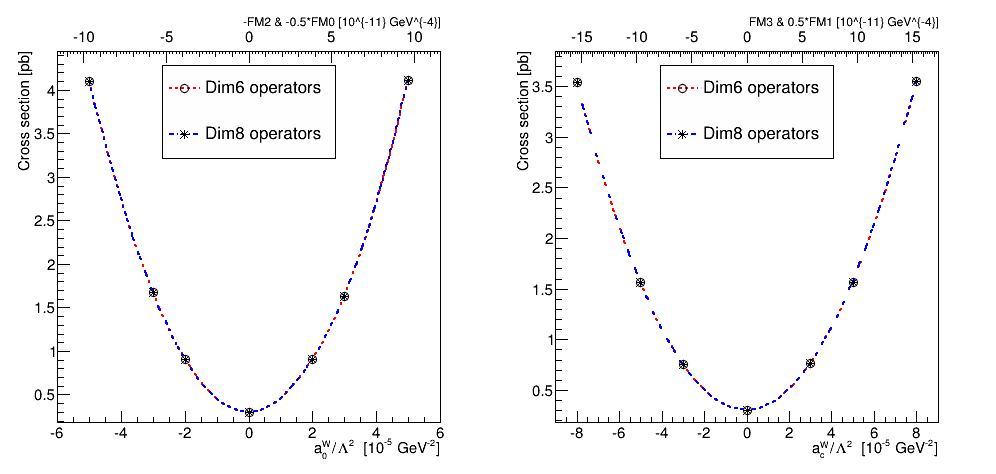
\includegraphics[width=0.8\textwidth]{figs/comp68.png}\\
  \caption{Checking the relations in Eq.s~\ref{dim6to8}}\label{comp}
\end{figure}

where $\dfrac{f_{M,i}}{\Lambda^4}$ are parameters of the linear formalism. We've checked this relation using the $p p \to W^+ W^- \gamma$ process without $W$ boson decay~\ref{comp}.

Moreover, there are more types of aQGC operators appearing in the linear
formalism which have never been tested before. Therefore, as a second
step, we investigate the ${\cal L}_{T,i}$ operators in the linear
formalism~\cite{Eboli:2006wa}, with new lorentz structures, which have
never been tested experimentally.

Therefore, concerning both vertex $WW\gamma \gamma$ and $WWZ\gamma$, the anomalous part of the total lagrangian \eqref{lagrangian} can be rewritten as

\begin{equation}\label{lagrangian}
{\cal L}_{AQGC} = \dfrac{a_0^W}{4 g^2} {\cal W}_{0}^{\gamma} + \dfrac{a_c^W}{4 g^2} {\cal W}_{c}^{\gamma} + \sum_i k_i^{W} {\cal W}_{i}^{Z} + {\cal L}_{T,0} + {\cal L}_{T,1} + {\cal L}_{T,2}
\end{equation}

% dimension 6 operators,  the $WW\gamma \gamma$ vertex, requiring only $U(1)_{EM}$ gauge invariance together with C and P conserved symmetry, arises from two basic Lorentz structures~\cite{Belanger:1999}
%\begin{eqnarray} 
%{\cal W}_{0}^{\gamma} &=& -\dfrac{e^{2}g^{2}}{2\Lambda^{2}}\; F_{\mu \nu} F^{\mu \nu} W^{+\alpha}W^{-}_{\alpha} \rightarrow i\dfrac{e^{2}g^{2}}{\Lambda^{2}}\; 2g_{\alpha \beta} (g_{\mu \nu} k_{1}k_{2}-k_{1\nu}k_{2\mu}) \nonumber \\
%&& \nonumber\\
%{\cal W}_{C}^{\gamma} &=& -\dfrac{e^{2}g^{2}}{4\Lambda^{2}}\; F_{\mu \nu} F^{\mu \alpha} \left( W^{+\nu}W^{-}_{\alpha} + W^{-\nu}W^{+}_{\alpha} \right) \rightarrow i\dfrac{e^{2}g^{2}}{2\Lambda^{2}}\;\left[ (g_{\mu\alpha}g_{\nu\beta}+g_{\nu\alpha}g_{\mu\beta})k_{1}\cdot k_{2} + g_{\mu\nu}(k_{2\beta}k_{1\alpha}+k_{1\beta}k_{2\alpha}) \right . \nonumber \\
%&& \left . \;\;\;\;\;\;\;\;\;\;\;\;\;\;\;\;\;\;\;\;\;\;\;\;\;\;\;\;\;\;\;\;\;\;\;\;\;\;\;\;\;\;\;\;\;\;\;\;\;\;\;\;\;\;\;\;\;\;\;\;\;\;\;\;\;\;\; - k_{2\mu}k_{1\alpha}g_{\nu\beta} - k_{2\beta}k_{1\nu}g_{\mu\alpha} - k_{2\alpha}k_{1\nu}g_{\mu\beta} - k_{2\mu}k_{1\beta}g_{\nu\alpha}   \right]
%\label{em_oper1}
%\end{eqnarray}
%while the $W^{+}W^{-}Z\gamma$ one has a maximum of 5 independent structures
%\begin{eqnarray}
%{\cal W}^{Z}_{0} &=& -\dfrac{e^{2}g^{2}}{\Lambda^{2}}\;F_{\mu\nu}Z^{\mu\nu}W^{+\alpha}W^{-}_{\alpha} \rightarrow i\dfrac{e^{2}g^{2}}{\Lambda^{2}}\; 2g_{\alpha \beta} (g_{\mu \nu} k_{1}k_{2}-k_{1\nu}k_{2\mu}) \nonumber\\
%&& \nonumber\\
%{\cal W}^{Z}_{C} &=& -\dfrac{e^{2}g^{2}}{2\Lambda^{2}}\;F_{\mu\nu}Z^{\mu\alpha} \left( W^{+\nu}W^{-}_{\alpha}+ W^{-\nu}W^{+}_{\alpha} \right) \rightarrow i\dfrac{e^{2}g^{2}}{2\Lambda^{2}}\;\left[ (g_{\mu\alpha}g_{\nu\beta}+g_{\nu\alpha}g_{\mu\beta})k_{1}\cdot k_{2} + g_{\mu\nu}(k_{2\beta}k_{1\alpha}+k_{1\beta}k_{2\alpha}) \right . \nonumber\\
%&& \nonumber\\
%&& \left .  \;\;\;\;\;\;\;\;\;\;\;\;\;\;\;\;\;\;\;\;\;\;\;\;\;\;\;\;\;\;\;\;\;\;\;\;\;\;\;\;\;\;\;\;\;\;\;\;\;\;\;\;\;\;\;\;\;\;\;\;\;\;\;\;\;\;\;- k_{2\mu}k_{1\alpha}g_{\nu\beta} - k_{2\beta}k_{1\nu}g_{\mu\alpha} - k_{2\alpha}k_{1\nu}g_{\mu\beta} - k_{2\mu}k_{1\beta}g_{\nu\alpha}   \right] \nonumber \\
%&&\nonumber\\
%{\cal W}^{Z}_{1} &=& -\dfrac{e^{2}g^{2}g_{Z}}{2\Lambda^{2}}\;F_{\mu\nu} \left( W^{+}_{\mu \nu}W^{-}_{\alpha}Z^{\alpha} + W^{-}_{\mu\nu}W^{+}_{\alpha}Z^{\alpha} \right) \rightarrow i\dfrac{eg^{2}g_{Z}}{\Lambda^{2}}\; \left ( (g_{\mu\alpha }k_{1}\cdot k_{+} - k_{+\mu}k_{1\alpha}  ) g_{\nu\beta}  + (g_{\mu\beta}k_{1}\cdot k_{-} - k_{-\mu} k_{1\beta}) g_{\nu\alpha} \right ) \nonumber\\
%&& \nonumber\\
%{\cal W}^{Z}_{2} &=& -\dfrac{eg^{2}g_{Z}}{2\Lambda^{2}}\;F_{\mu\nu} \left( W^{+}_{\mu \alpha}W^{-}_{\alpha}Z^{\nu} + W^{-}_{\mu\alpha}W^{+\alpha}Z^{\nu} \right) \rightarrow i\dfrac{eg^{2}g_{Z}}{2\Lambda^{2}}\; \left [  (k_{1}\cdot k_{+} + k_{1}\cdot k_{-})g_{\mu\nu}g_{\alpha\beta} - (k_{1\alpha}k_{+\beta} + k_{1\beta}k_{-\alpha})g_{\mu\nu} \right . \nonumber \\
%&& \nonumber \\
%&& \left .  \;\;\;\;\;\;\;\;\;\;\;\;\;\;\;\;\;\;\;\;\;\;\;\;\;\;\;\;\;\;\;\;\;\;\;\;\;\;\;\;\;\;\;\;\;\;\;\;\;\;\;\;\;\;\;\;\;\;\;\;\;\;\;\;\;\;\; - (k_{+\mu}+k_{-\mu})k_{1\nu}g_{\alpha \beta} + (k_{+\beta} g_{\mu\alpha} + k_{-\alpha}g_{\mu\beta} )k_{1\nu}\right] \nonumber \\
%&& \nonumber \\
%{\cal W}^{Z}_{3} &=& -\dfrac{eg^{2}g_{Z}}{2\Lambda^{2}}\;F_{\mu\nu} \left( W^{+}_{\mu \alpha}W^{-}_{\nu}Z^{\alpha} + W^{-}_{\mu\alpha}W^{+}_{\nu}Z^{\alpha} \right) \rightarrow i\dfrac{eg^{2}g_{Z}}{2\Lambda^{2}}\;   ( k_{1}\cdot k_{+} g_{\mu\beta}g_{\nu\alpha} + k_{1}\cdot k_{-} g_{\mu\alpha}g_{\nu\beta} + (k_{+\nu} - k_{-\nu})k_{1\beta} g_{\mu\alpha}  \nonumber \\
%&& \nonumber \\
%&&  \;\;\;\;\;\;\;\;\;\;\;\;\;\;\;\;\;\;\;\;\;\;\;\;\;\;\;\;\;\;\;\;\;\;\;\;\;\;\;\;\;\;\;\;\;\;\;\;\;\;\;\;\;\;\;\;\;\;\;\;\;\;\;\;\;\;\;- (k_{+\nu}-k_{-\nu})k_{1\alpha}g_{\mu\beta} - k_{+\mu}k_{1\beta} g_{\nu\alpha} - k_{-\mu}k_{1\alpha}g_{\nu\beta})
%\label{em_oper2}
%\end{eqnarray}
%where $g=e/s_{W}$ and $g_{Z}=e/c_{W}s_{W}$.

%In order to embed the set of operators \eqref{em_oper1} and \eqref{em_oper2}  in manifestly $SU(2)\times U(1)$ gauge invariant and $SU(2)_{C}$ symmetric operators (as well as C and P conserving),  one uses the chiral Lagrangian approach which assumes no Higgs in the spectrum (a Higgsless scenario).

%In this scenario, concerning the purely bosonic sector, the $SU(2)$ kinetic term that originates the standard tree-level gauge self-coulplings is
%\begin{equation}
%{\cal L}_{Gauge} = -\dfrac{1}{2} \left[ \mbox{Tr}(\mathbf{W}_{\mu\nu}\mathbf{W^{\mu\nu}} +\mbox{Tr}(\mathbf{B}_{\mu\nu}\mathbf{B}^{\mu\nu} )  \right]
%\end{equation}
% where the $SU(2)$ gauge fields are $\mathbf{W}_{\mu}=W_{\mu}^{i}\tau^{i}$ and the hypercharge is denoted by $\mathbf{B}_{\mu}=\tau_{3}B_{\mu}$. The normalization for the Pauli matrices is $\mbox{Tr}(\tau^{i}\tau^{j})=2\delta^{ij}$. The field strength is  defined as
%\begin{equation}
%\mathbf{W}_{\mu\nu} = \dfrac{1}{2}\left( \partial_{\mu}\mathbf{W}_{\nu} - \partial_{\nu}\mathbf{W}_{\mu} + \dfrac{i}{2}\;g\;[\mathbf{W}_{\mu},\mathbf{W}_{\nu}]   \right) = \dfrac{\tau^{i}}{2} \left ( \partial_{\mu}W_{\nu} - \partial_{\nu}W_{\mu} -\;g\;\epsilon^{ijk} W_{\mu}^{j} W_{\nu}^{k}  \right )
%\end{equation} 

%Choosing a matrix field $\Sigma$ to acommodate the Goldstone bosons $w^{i}$ , with $i=1,2,3$, we have
%\begin{equation}
%\Sigma = \exp{i(\frac{w^{i}\tau^{i}}{v})}\;\;\mbox{with covariant derivative as}\;\; D_{\mu}\Sigma = \partial_{\mu}\Sigma+ \frac{i}{2} (g\mathbf{W}_{\mu}\Sigma - g'\;\mathbf{B}_{\mu}\Sigma \tau_{3}  )
%\end{equation}
%where $v=246$~GeV , $g=e/s_{W}$ and $g'=e/c_{W}$.


%Defining the matrix field $\mathbf{V}_{\mu}=(D_{\mu}\Sigma)\Sigma^{\dagger}$, we note that in the unitary gauge $\mathbf{V}_{\mu}$ corresponds to the triplet of the massive gauge bosons $W^{\pm},Z$. Indeed, in the unitary gauge $\Sigma=\mathbf{1}$ and then $\mathbf{V}_{\mu}=D_{\mu}\mathbf{1}=i (g\mathbf{W}_{\mu}-g'\mathbf{B}_{\mu})$ where $\mathbf{W}_{\mu}= \dfrac{\vec{W}_{\mu}\cdot \vec{\tau}}{2}$ and  $\mathbf{B}_{\mu}= \dfrac{B_{\mu}\cdot \tau_{3}}{2}$.

%The NLO in the chiral Lagrangian approach (dimension 4) gives genuine quartic couplings involving massive vector bosons $WWWW$, $WWZZ$, $ZZZZ$ which are out of the scope of our analysis. No photonic operators arises in this perturbation order expansion.

%Photonic operators only appear at NNLO (dimension 6).  Although these NNLO operators also involve quartic couplings between massive gauge bosons, for the sake of simplicity we restrict our list only for the photonic part we are interested in.
%\begin{eqnarray}
%&&\dfrac{k_{0,C}^{w}}{\Lambda^{2}}\;g^{2}\;\mbox{Tr}(\mathbf{W}_{\mu\nu}\mathbf{W}^{\mu\nu})\mbox{Tr}(\mathbf{V}^{\alpha}\mathbf{V}_{\alpha}) + \dfrac{k_{0,C}^{b}}{\Lambda^{2}}\;g^{\prime 2}\;\mbox{Tr}(\mathbf{B}_{\mu\nu}\mathbf{B}^{\mu\nu})\mbox{Tr}(\mathbf{V}^{\alpha}\mathbf{V}_{\alpha}) + \dfrac{k_{0,C}^{m}}{\Lambda^{2}}\;gg^{\prime}\;\mbox{Tr}(\mathbf{W}_{\mu\nu}\mathbf{B}^{\mu\nu})\mbox{Tr}(\mathbf{V}^{\alpha}\mathbf{V}_{\alpha}) \nonumber \\
%&+&\dfrac{k_{1}^{w}}{\Lambda^{2}}\;g^{2}\;\mbox{Tr}(\mathbf{W}_{\mu\nu}\mathbf{V}^{\alpha})\mbox{Tr}(\mathbf{W}_{\mu\nu}\mathbf{V}_{\alpha}) + \dfrac{k_{2}^{w}}{\Lambda^{2}}\;g^{2}\;\mbox{Tr}(\mathbf{W}_{\mu\nu}\mathbf{V}^{\nu})\mbox{Tr}(\mathbf{W}_{\mu\alpha}\mathbf{V}_{\alpha} + \dfrac{k_{3}^{w}}{\Lambda^{2}}\;g^{2}\;\mbox{Tr}(\mathbf{W}_{\mu\nu}\mathbf{V}_{\alpha})\mbox{Tr}(\mathbf{W}^{\mu\alpha}\mathbf{V}^{\nu})\nonumber \\
%&+&\dfrac{k_{1}^{m}}{\Lambda^{2}}\;gg^{\prime}\;\mbox{Tr}(\mathbf{W}_{\mu\nu}\mathbf{V}^{\alpha})\mbox{Tr}(\mathbf{B}_{\mu\nu}\mathbf{V}_{\alpha}) +\dfrac{k_{2}^{m}}{\Lambda^{2}}\;gg^{\prime}\;\mbox{Tr}(\mathbf{W}_{\mu\nu}\mathbf{V}^{\nu})\mbox{Tr}(\mathbf{B}_{\mu\alpha}\mathbf{V}_{\alpha}) + \dfrac{k_{3}^{m}}{\Lambda^{2}}\;gg^{\prime}\;\mbox{Tr}(\mathbf{W}_{\mu\nu}\mathbf{V}^{\alpha})\mbox{Tr}(\mathbf{B}_{\mu\alpha}\mathbf{V}_{\nu}) \nonumber \\
%\label{dim6}
%\end{eqnarray}

%In this way, for the photonic vertices $WW\gamma \gamma$ and $WWZ\gamma$, looking only at features of the non-linearly built dimension 6 operators of the set \eqref{dim6}, we can construct the lagrangians ${\cal L}_{0}^{6}$ and ${\cal L}_{C}^{6}$ as follows

%\begin{equation}
% {\cal L}_{\{0,C\}}^{6}= (k_{0,C}^{w}+  k_{0,C}^{b} + k_{0,C}^{m}) {\cal W}_{0}^{\gamma}  + (\dfrac{c_{W}}{s_{W}} k_{0,C}^{w}- \dfrac{s_{W}}{c_{W}} k_{0,C}^{b} +c_{ZW}k_{0,C}^{m}) {\cal W}_{0}^{Z}
%\end{equation}
%where
%\[
%c_{ZW}\equiv \mbox{cotg}{(2\theta_{W})} = \dfrac{c^{2}_{W}- s^{2}_{W}}{2c_{W}s_{W}}.
%\]

%Moreover, the vertex $WWZ\gamma$ has other specific contributing terms, we may name as ${\cal L}_{Z}^{6}$, like 
%\begin{equation}
% {\cal L}_{Z}^{6}= (k_{1}^{w}+ k_{1}^{m}){\cal W}_{1}^{Z} +(k_{2}^{w} + k_{2}^{m}){\cal W}_{2}^{Z} + (k_{3}^{w} + k_{3}^{m}){\cal W}_{3}^{Z}
%\label{LZ}
%\end{equation}

%Therefore, while for $WW\gamma \gamma$ we can compute "only" its corresponding part at ${\cal L}_{0}$ and ${\cal L}_{C}$,  for the $WWZ\gamma$ vertex we have to consider, beyond its corresponding part at  ${\cal L}_{0}$ and ${\cal L}_{C}$, also the ${\cal L}_{Z}$ contribution.

%The LEP collaboration has adopted the set of operators \eqref{em_oper1} to infer constraints on their $a_{0}$ and $a_{C}$ parameters. In order to make a comparison with these previous results,  we may relate parameters conveniently. This goal in mind, by assuming $k_{1,2,3}^{w,m}=0$ (since they do not contribute to $WW\gamma \gamma$) and the constraints
%\begin{equation}
%k_{0,C}^{w} = k_{0,C}^{\gamma} s^{2}_{W} \;\;\;\;\;, \;\;\;\;\; k_{0,C}^{b} = k_{0,C}^{\gamma} c^{2}_{W},  
%\end{equation}
%we obtain only two independent parameters controlling $WW\gamma\gamma$ vertex, making the following contact with the operators analyzed by LEP
%\begin{equation}
%a_{0,C}=4g^{2}(k_{0,C}^{b}+k_{0,C}^{w}+k_{0,C}^{m}) = 4g^{2}k_{0,C}^{\gamma}.
%\end{equation}

% In general, using a manifestly gauge invariant and $SU(2)_{C}$ symmetric approach, the operators which contribute to $WW\gamma\gamma$, $k_{0,C}^{w,b,m}$ do in general induce a $WWZ\gamma$ vertex as well. Therefore, with $k_{1,2,3}^{w,m}=0$ the general condition for the vanishing of $WWZ\gamma$ is
%\begin{equation}
%2k_{0,C}^{w}+k_{0,C}^{m}=2\sin^{2}{\theta_{W}}\;(k_{0,C}^{b}+k_{0,C}^{w}+k_{0,C}^{m})
%\end{equation}
%with
%\begin{equation}
%k_{0,C}^{b}+k_{0,C}^{w}+k_{0,C}^{m} \neq 0
%\end{equation}
%of course not making the $VV\gamma \gamma$ vanish.

%On the other hand one can also arrange the operators such that $SU(2)_{C}$ $WW\gamma\gamma$ couplings vanish so that effectively $a_{0,C}=0$ but not the quartic $WWZ\gamma$ one. For instance, with all $k_{1,2,3}=0$ , this can achieved by having $k_{0,C}^{b}=-k_{0,C}^{w}$.

%Up to now we have adopted an effective lagrangian approach which does not assume a Higgs-like field on the spectrum of the theory. Nevertheless, any operator can be made gauge invariant with the Higgs presence, only changing the hierarchy in the couplings changes, realizing the symmetry linearly. 

%Assuming a scenario where the low energy spectrum contains a light Higgs boson, we
%can choose a linear realization of the symmetry breaking in the form of
%the usual scalar doublet field $\Phi$,
%\[
%\Phi = \dfrac{1}{\sqrt{2}}\begin{pmatrix} 0 & v+ H \end{pmatrix}^{T},
%\]
%where $v=246$~GeV.

%The basic blocks for constructing the operators which can modify the 
%quartic gauge boson vertices are the covariant derivative of the Higgs
%field $D_{\mu}\Phi$,  the $SU(2)_{L}$ field strength 
%$\hat{W}_{\mu \nu}$, and the $U(1)_{Y}$ field strength 
%$\hat{B}_{\mu \nu}$ listed bellow.

%\begin{eqnarray}
%\Phi &\mbox{, transforming as} & \Phi^{\prime}=U\Phi \\
%D_{\mu}\Phi &\mbox{, transforming as} & D^{\prime}_{\mu}\Phi^{\prime}=UD_{\mu}\Phi \\
%\hat{W}_{\mu \nu}\equiv i\frac{g}{2}\sum_{j}W^{j}_{\mu \nu}\sigma^{j} &\mbox{, transforming as} & \hat{W}^{\prime}_{\mu \nu}= U\hat{W}_{\mu\nu}U^{\dagger} \\
%\hat{B}_{\mu \nu}=i\frac{g^{\prime}}{2}B_{\mu \nu} &\mbox{, transforming as} & B^{\prime}_{\mu \nu}=B_{\mu \nu}
%\label{linear_blocks}
%\end{eqnarray}

%where the covariant derivative is given by 
%\[
%D_{\mu} = \partial_{\mu}+i\frac{g}{2}W^{j}_{\mu}\sigma^{j}+i\frac{g^{\prime}}{2}B_{\mu}, 
%\]

%\[
%\left[ D_{\mu}, D_{\nu} \right]=\hat{W}_{\mu \nu}+\hat{B}_{\mu \nu},
%\]

%and

%\begin{eqnarray}
%W^{j}_{\mu \nu}&=&\partial _{\mu}W^{j}_{\nu}-\partial_{\nu}W^{j}_{\mu}+g\epsilon_{jkm}W_{\mu}^{k}W_{\nu}^{m},\\
%B_{\mu \nu}&=& \partial_{\mu}B_{\nu}-\partial_{\nu}B_{\mu}.
%\end{eqnarray}

%In this context, the lowest dimension operator that leads to pure 
%quartic interactions (not exhibiting two or three real gauge boson 
%vertices) is dimension 8. Many CP conserving effective dim-8 operators 
%were already listed elsewhere~\cite{Eboli:2006wa}. Here we have 
%manipulated operators showing only $WW\gamma\gamma$ and $WWZ\gamma$ 
%vertices.

%From the linear realized symmetry scenario emerges dimension 8 operators which shows a trivial equivalence with the already built dimension 6 ones, ${\cal L}_{\{0,C\}}^{6}$,  as
%\begin{eqnarray}
%{\cal L}_{0}^{8} &=& g^{\prime 2}\; \dfrac{Q_{0}^{b}}{\Lambda^{4}} (D_{\beta}\Phi)(D^{\beta}\Phi)^{\dagger} B_{\mu\nu}B^{\mu\nu} + g^{2}\; \dfrac{Q_{0}^{w}}{\Lambda^{4}} (D_{\beta}\Phi)(D^{\beta}\Phi)^{\dagger} W^{i}_{\mu\nu}W^{i\mu\nu} + gg^{\prime}\; \dfrac{Q_{0}^{m}}{\Lambda^{4}} (D_{\beta}\Phi)(D^{\beta}\Phi)^{\dagger} W^{3}_{\mu\nu}B^{\mu\nu}  \nonumber\\
%&& \nonumber\\
%&& \nonumber\\
%{\cal L}_{C}^{8} &=& g^{\prime 2}\; \dfrac{Q_{C}^{b}}{2\Lambda^{4}} (D^{\alpha}\Phi)(D_{\beta}\Phi)^{\dagger} B_{\mu\alpha}B^{\mu\beta} + g^{2}\; \dfrac{Q_{C}^{w}}{2\Lambda^{4}} (D^{\alpha}\Phi)(D_{\beta}\Phi)^{\dagger} W^{i}_{\mu\alpha}W^{i\mu\beta} + gg^{\prime}\; \dfrac{Q_{C}^{m}}{2\Lambda^{4}} (D^{\alpha}\Phi)(D_{\beta}\Phi)^{\dagger} W^{3}_{\mu\alpha}B^{\mu\beta}\nonumber \\
%\label{dim8_belanger}
%\end{eqnarray}

%where one can make a trivial correspondence both scenario between parameters as 
%\begin{equation}
%\dfrac{Q^{b,w,m}_{0,C}}{\Lambda^{2}} =-\dfrac{1}{2}\dfrac{g^{2}}{M_{W}^{2}}\; k_{0,C}^{b,w,m}.
%\label{relation}
%\end{equation}

%To measure the deviation from the SM lagrangian, we are interested on the following effective lagrangian based upon the operators listed so far

%\begin{equation}
%{\cal L}_{Total}= {\cal L}_{SM} + {\cal L}_{ANOM}
%\label{lagrangian}
%\end{equation}

%which contributes to the squared matriz element as
%\begin{equation}
%|{\cal M}_{Total}|^{2}= |{\cal M}_{SM}+{\cal M}_{AQGC} |^{2} =  |{\cal M}_{SM}|^{2}+|{\cal M}_{AQGC} |^{2} + ({\cal M}^{*}_{SM}{\cal M}_{AQGC} + {\cal M}_{SM}{\cal M}^{*}_{AQGC})
%\end{equation}
%, $M_{W}=gv/2$, $M_{Z}=g_{Z}v/2$ with
%Since the squared matrix element is proportional to the cross section then we may parameterize the total cross section for the process $pp\to l\nu_{ll}jj\gamma$ as a quadratic function
%\begin{equation}
%\sigma_{total} \equiv \sigma_{SM} + \beta\sigma_{INT} +\beta^{2}\sigma_{AQGC}
%\end{equation}
%where $\sigma_{SM}$,  $\sigma_{INT}$, $\sigma_{AQGC}$ are  Standard Model cross section, interference between the SM and the anomalous contributions and the pure anomalous cross section, respectively.

%%Therefore, concerning both vertex $WW\gamma \gamma$ and $WWZ\gamma$, the anomalous part of the total lagrangian \eqref{lagrangian} may be rewritten as

%\begin{equation}
%{\cal L}_{AQGC}= {\cal L}_{0}^{6} + {\cal L}_{C}^{6} +{\cal L}_{Z}^{6} + {\cal L}_{T0,5} + {\cal L}_{T1,6} + {\cal L}_{2,7}
%\end{equation}
%where ${\cal L}_{Z}^{6}={\cal L}_{1}+{\cal L}_{2}+{\cal L}_{3}$ is the expression  \eqref{LZ} and the additional operators named ${\cal L}_{T0,5}$, ${\cal L}_{T1,6}$ and ${\cal L}_{2,7}$, listed below in the set of Eqs. \eqref{lt_operators}, are linearly realized dimension 8 effective operators which were not yet probed before.

%In the following we listed other dimension 8 operators related to our analysis~~\cite{Eboli:2006wa}.

%\begin{itemize}
%\item Structure compatible with ${\cal L}_{0}^{8}$
%\begin{eqnarray}
%{\cal L}_{M,\{2+0+4\}} &=& \dfrac{f_{M2}}{\Lambda^{4}}\;\mbox{Tr}\left[ \mathbf{B}_{\mu\nu} \mathbf{B}^{\mu\nu}\right] \times \left[  (D_{\beta}\Phi)^{\dagger} D^{\beta}\Phi \right] + \dfrac{f_{M0}}{\Lambda^{4}}\;\mbox{Tr}\left[ \mathbf{W}_{\mu\nu} \mathbf{W}^{\mu\nu}\right] \times \left[  (D_{\beta}\Phi)^{\dagger} D^{\beta}\Phi \right] \nonumber \\
%&& \nonumber \\
%&&+ \dfrac{f_{M4}}{\Lambda^{4}}\;\left[  (D_{\beta}\Phi)^{\dagger} \mathbf{W}^{\beta\nu}  D^{\mu}\Phi \right] \times \mathbf{B}^{\beta\nu} \nonumber \\
%&& \nonumber\\
%&\rightarrow&  i\; g^{2}m_{W}^{2}s^{2}_{W} \; \dfrac{(f_{M2}+2f_{M0}+f_{M4})}{\Lambda^{4}}\; g^{\mu\nu} (g^{a_{1}a_{2}}p_{\lambda_{1}}p_{\lambda_{2}} - p_{\lambda_{2}}^{a_{1}} p_{\lambda_{1}}^{a_{2}})
%\label{dim8_a}
%\end{eqnarray}

%\item Structure compatible with ${\cal L}_{C}^{8}$
%\begin{eqnarray}
%{\cal L}_{M,\{3+1+5\}} &=& \dfrac{f_{M3}}{\Lambda^{4}}\;\mbox{Tr}\left[ \mathbf{B}_{\mu\nu} \mathbf{B}^{\nu\beta}\right] \times \left[  (D_{\beta}\Phi)^{\dagger} D^{\mu}\Phi \right] + \dfrac{f_{M1}}{\Lambda^{4}}\;\mbox{Tr}\left[ \mathbf{W}_{\mu\nu} \mathbf{W}^{\nu\beta}\right] \times \left[  (D_{\beta}\Phi)^{\dagger} D^{\mu}\Phi \right] \nonumber \\
%&& \nonumber \\
%&& + \dfrac{f_{M5}}{\Lambda^{4}}\;\left[  (D_{\mu}\Phi)^{\dagger} \mathbf{W}^{\beta\nu}  D^{\nu}\Phi \right] \times \mathbf{B}^{\beta\nu} \nonumber \\
%&& \nonumber \\
%&\rightarrow& i \; g^{2}m_{W}^{2}s^{2}_{W} \; \dfrac{((1/4)f_{M3}+(1/2)f_{M1}+(1/4)f_{M5})}{\Lambda^{4}}\; \left (   - p_{\lambda_{2}}^{a_{1}} ( p^{\nu}_{\lambda_{1}}g^{a_{2}\mu} + p_{\lambda_{1}}^{\mu}g^{a_{2}\nu})  \right . \nonumber \\
%&& \nonumber \\
%&& \left .-  p_{\lambda_{1}}^{a_{2}} ( p^{\nu}_{\lambda_{2}}g^{a_{1}\mu} + p_{\lambda_{2}}^{\mu}g^{a_{1}\nu})+ g^{a_{1}a_{2}} ( p^{\mu}_{\lambda_{1}}p_{\lambda_{2}}^{\nu} + p_{\lambda_{1}}^{\nu}  p^{\mu}_{\lambda_{2}}) + p_{\lambda_{1}}\cdot p_{\lambda_{2}} ( g^{a_{1}\mu}g^{a_{2}\nu} +g^{a_{1}\nu}g^{a_{2}\mu} ) \right )\nonumber \\
%\label{dim8_b}
%\end{eqnarray}

%\item Not directly related with dimension 6 ones.
%\begin{eqnarray}
%{\cal L}_{T,\{0+5\}} &=&\dfrac{f_{T0}}{\Lambda^{4}}\;\mbox{Tr}\left[ \mathbf{W}_{\mu\nu} \mathbf{W}^{\mu\nu}\right] \times \mbox{Tr}\left[ \mathbf{W}_{\alpha\beta} \mathbf{W}^{\alpha\beta}\right] +  \dfrac{f_{T5}}{\Lambda^{4}}\;\mbox{Tr}\left[ \mathbf{W}_{\mu\nu} \mathbf{W}^{\mu\nu}\right] \times \mathbf{B}_{\alpha\beta} \mathbf{B}^{\alpha\beta} \nonumber \\
%&\rightarrow& i \;s^{2}_{W}g^{4}\;\dfrac{(8f_{T0}+2f_{T5})}{\Lambda^{4}}\; [(p_{\gamma_{2}}^{a_{1}}  p_{\gamma_{1}}^{a_{2}} - g^{a_{1}a_{2}} p_{\gamma_{1}}\cdot p_{\gamma_{2}}) (p_{-}^{\mu}p_{+}^{\nu}-g^{\nu\mu}p_{-}\cdot p_{+})] \nonumber \\
%&& \nonumber \\
%&& \nonumber \\
%{\cal L}_{T,\{1+6\}} &=& \dfrac{f_{T1}}{\Lambda^{4}}\;\mbox{Tr}\left[ \mathbf{W}_{\alpha\nu} \mathbf{W}^{\mu\beta}\right] \times \mbox{Tr}\left[ \mathbf{W}_{\mu\beta} \mathbf{W}^{\alpha\nu}\right] +  \dfrac{f_{T6}}{\Lambda^{4}}\;\mbox{Tr}\left[ \mathbf{W}_{\alpha\nu} \mathbf{W}^{\mu\beta}\right] \times \mathbf{B}_{\mu\beta} \mathbf{B}^{\alpha\nu} \nonumber\\
%&& \nonumber \\
%&\rightarrow& i\;s^{2}_{W}g^{4} \;\dfrac{(4f_{T1}+f_{T6})}{\Lambda^{4}}\; \left ( (p_{+}^{a_{1}}p_{\gamma_{1}}^{\mu} - g^{a_{1}\mu}p_{\gamma_{1}}\cdot p_{+} ) (p_{-}^{a_{2}}p_{\gamma_{2}}^{\nu} - g^{a_{2}\nu}p_{\gamma_{2}}\cdot p_{-} ) \right . \nonumber \\
%&& \nonumber \\
%&& + \left . (p_{-}^{a_{1}}p_{\gamma_{1}}^{\nu} - g^{a_{1}\nu}p_{\gamma_{1}}\cdot p_{-}) + (p_{+}^{a_{2}}p_{\gamma_{2}}^{\mu} - g^{a_{2}\mu}p_{\gamma_{2}}\cdot p_{+} ) \right) \nonumber \\
%&& \nonumber \\ 
%&& \nonumber \\
%{\cal L}_{T,\{2+7\}} &=& \dfrac{f_{T2}}{\Lambda^{4}}\;\mbox{Tr}\left[ \mathbf{W}_{\alpha\mu} \mathbf{W}^{\mu\beta}\right] \times \mbox{Tr}\left[ \mathbf{W}_{\beta\nu} \mathbf{W}^{\nu\alpha}\right] + \dfrac{f_{T7}}{\Lambda^{4}}\;\mbox{Tr}\left[ \mathbf{W}_{\alpha\mu} \mathbf{W}^{\mu\beta}\right] \times \mathbf{B}_{\beta\nu} \mathbf{B}^{\nu\alpha} \nonumber \\
%&& \nonumber \\
%&\rightarrow& i\;s^{2}_{W}g^{4} \;\dfrac{(f_{T2}+(1/4)f_{T7})}{\Lambda^{4}}\; \left \{ g^{a_{1}a_{2}}g^{\mu\nu} (p_{\lambda_{1}}\cdot p_{+}\;p_{\lambda_{2}} \cdot p_{-} + p_{\lambda_{1}}\cdot p_{-}\;p_{\lambda_{2}}\cdot p_{+}) \right .\nonumber \\
%&& \nonumber \\
%&& g^{\mu\nu} \left[ - p^{a_{1}}_{\lambda_{2}} ( p_{+}^{a_{2}}\;p_{\lambda_{1}} \cdot p_{-} + p^{a_{2}}_{-} p_{\lambda_{1}}\cdot p_{+} ) + p_{+}^{a_{1}} ( p_{-}^{a_{2}}\; p_{\lambda_{1}} \cdot p_{\lambda_{2}}  -  p_{\lambda_{1}}^{a_{2}}\; p_{\lambda_{2}}\cdot p_{-}  ) \right .\nonumber \\
%&& \nonumber \\
%&& \left .+p^{a_{1}}_{-} ( p_{+}^{a_{2}}\; p_{\lambda_{1}}\cdot p_{\lambda_{2}} -  p_{\lambda_{1}}^{a_{2}}\;p_{\lambda_{2}}\cdot p_{+}) \right] \nonumber \\
%&& \nonumber \\
%&& g^{a_{1}\mu}g^{a_{2}\nu} p_{\lambda_{1}}\cdot p_{\lambda_{2}} \; p_{-} \cdot p_{+} + 
%g^{a_{1}\nu}g^{a_{2}\mu} p_{\lambda_{1}}\cdot p_{\lambda_{2}}\; p_{-}\cdot p_{+} \nonumber\\
%&& \nonumber \\
%&&  - g^{a_{1}a_{2}} \left[  p^{\nu}_{+} ( p_{\lambda_{2}}^{\mu}\;p_{\lambda_{1}} \cdot p_{-} + p^{\mu}_{\lambda_{1}}\; p_{\lambda_{2}}\cdot p_{-} ) + p_{-}^{\mu} ( p_{\lambda_{2}}^{\nu}\; p_{\lambda_{1}} \cdot p_{+}  +  p_{\lambda_{1}}^{\nu}\; p_{\lambda_{2}}\cdot p_{+}  ) \right .\nonumber \\
%&& \nonumber \\
%&& \left. -p_{-}\cdot p_{+} \; ( p_{\lambda_{1}}^{\mu}p_{\lambda_{2}}^{\nu} + p_{\lambda_{1}}^{\nu} + p_{\lambda_{2}}^{\mu}) \right] \nonumber \\
%&& \nonumber \\
%&& - g^{a_{2}\mu} ( p_{-}^{a_{1}}p_{+}^{\nu}\;p_{\lambda_{1}}\cdot p_{\lambda_{2}} + p_{\lambda_{2}}^{a_{1}} ( p_{\lambda_{1}}^{\nu}p_{-}\cdot p_{+} - p_{+}^{\nu} p_{\lambda_{1}} \cdot p_{-} ) ) \nonumber \\
%&& \nonumber \\
%&& -  g^{a_{1}\mu} ( p_{-}^{a_{2}}p_{+}^{\nu}\;p_{\lambda_{1}}\cdot p_{\lambda_{2}} + p_{\lambda_{1}}^{a_{2}} ( p_{\lambda_{2}}^{\nu}p_{-}\cdot p_{+} - p_{+}^{\nu} p_{\lambda_{2}} \cdot p_{-} ) ) \nonumber \\
%&& \nonumber \\
%&& - g^{a_{2}\nu} ( p_{+}^{a_{1}}p_{-}^{\mu}\;p_{\lambda_{1}}\cdot p_{\lambda_{2}} + p_{\lambda_{2}}^{a_{1}} ( p_{\lambda_{1}}^{\mu}p_{-}\cdot p_{+} - p_{-}^{\nu} p_{\lambda_{1}} \cdot p_{+} ) ) \nonumber \\
%&& \nonumber \\
%&& - g^{a_{1}\nu} ( p_{+}^{a_{2}}p_{-}^{\mu}\;p_{\lambda_{1}}\cdot p_{\lambda_{2}} + p_{\lambda_{1}}^{a_{2}} ( p_{\lambda_{2}}^{\mu}p_{-}\cdot p_{+} - p_{-}^{\mu} p_{\lambda_{2}} \cdot p_{+} ) ) \nonumber \\
%&& \nonumber \\
%&& + \left . p_{\lambda_{2}}^{a_{1}} p_{-}^{a_{2}}  p_{\lambda_{1}}^{\mu} p_{+}^{\nu} + p_{-}^{a_{1}} p_{\lambda_{1}}^{a_{2}}  p_{\lambda_{2}}^{\mu} p_{+}^{\nu} + p_{\lambda_{2}}^{a_{1}} p_{+}^{a_{2}}  p_{\lambda_{1}}^{\nu} p_{-}^{\nu} + p_{+}^{a_{1}} p_{\lambda_{1}}^{a_{2}}  p_{\lambda_{2}}^{\nu} p_{-}^{\mu}   \right \}
%\label{lt_operators}
%\end{eqnarray}

%\end{itemize}

%\begin{figure}[!htb]
%\centering
%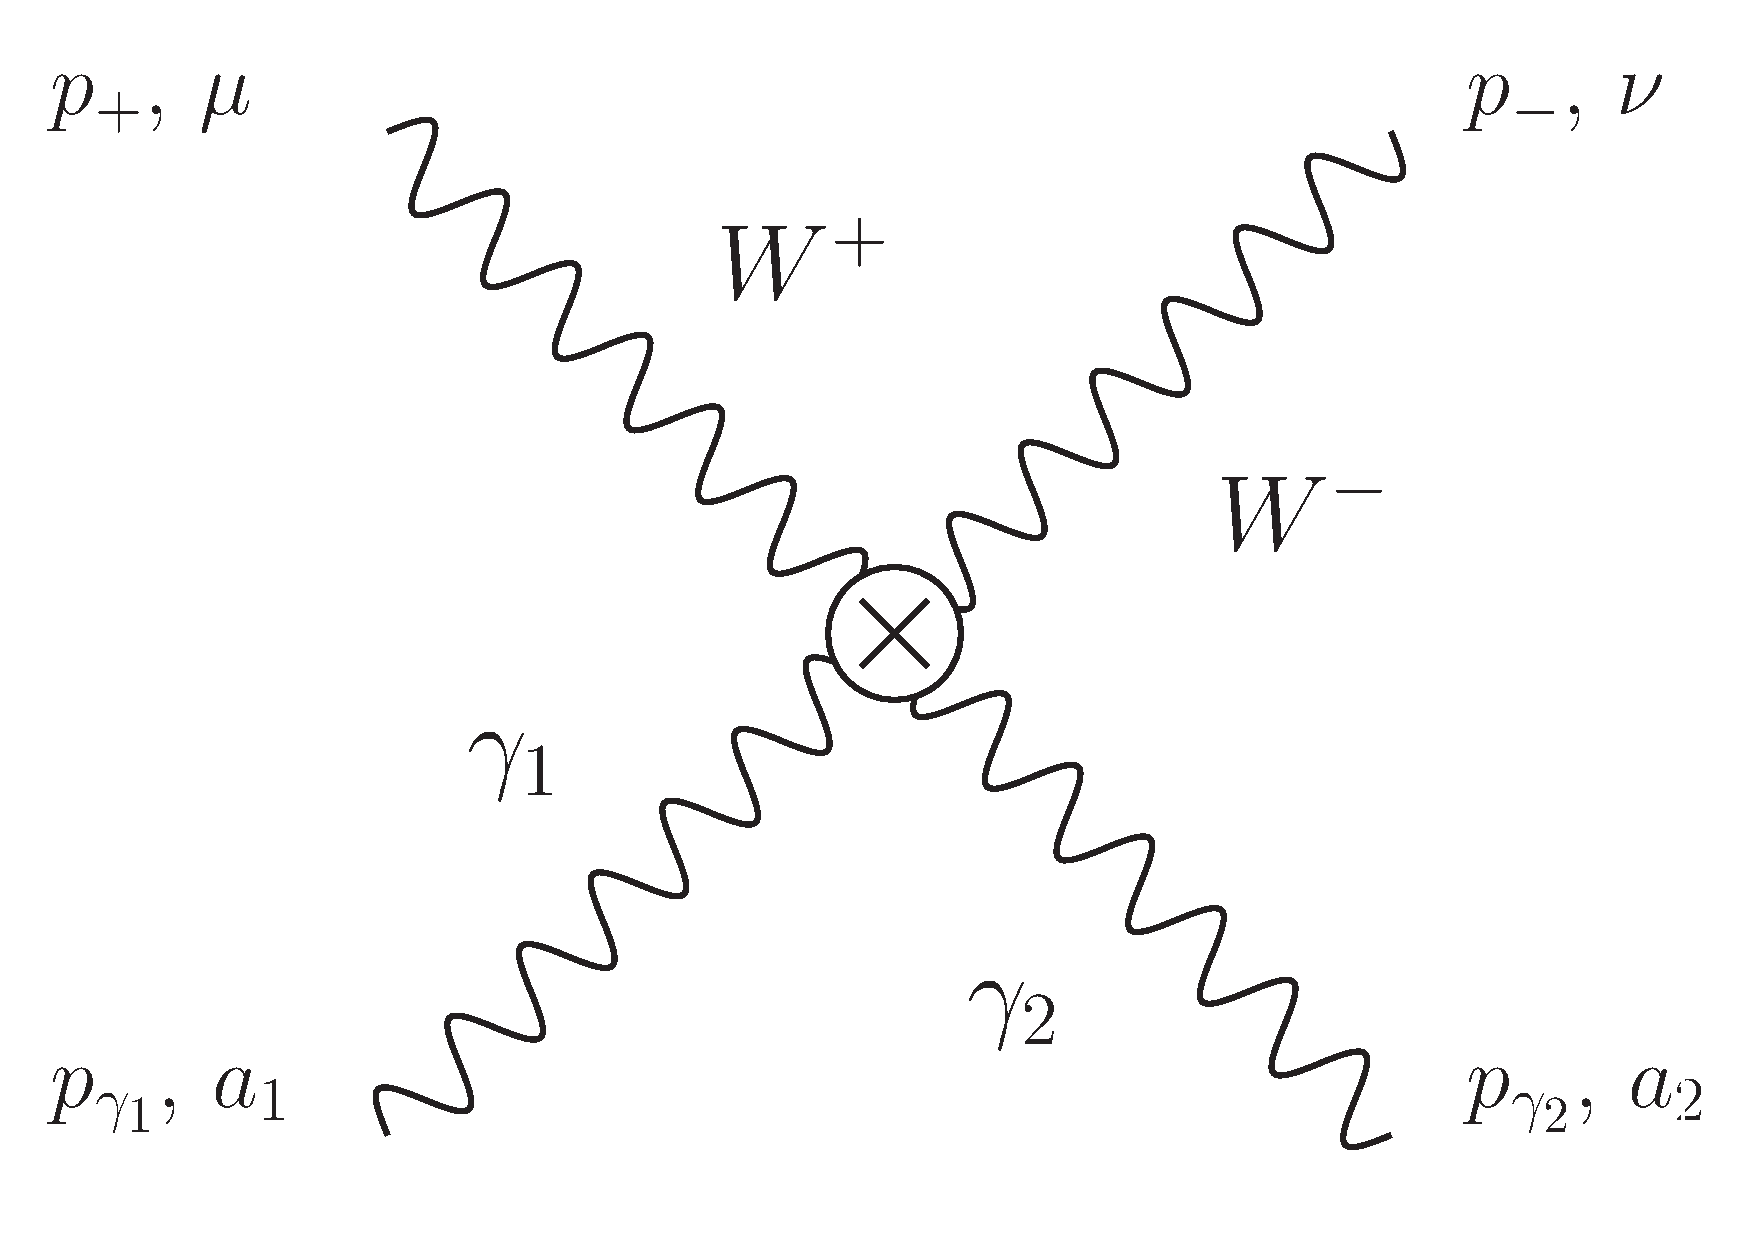
\includegraphics[scale=0.25]{WWAA}
%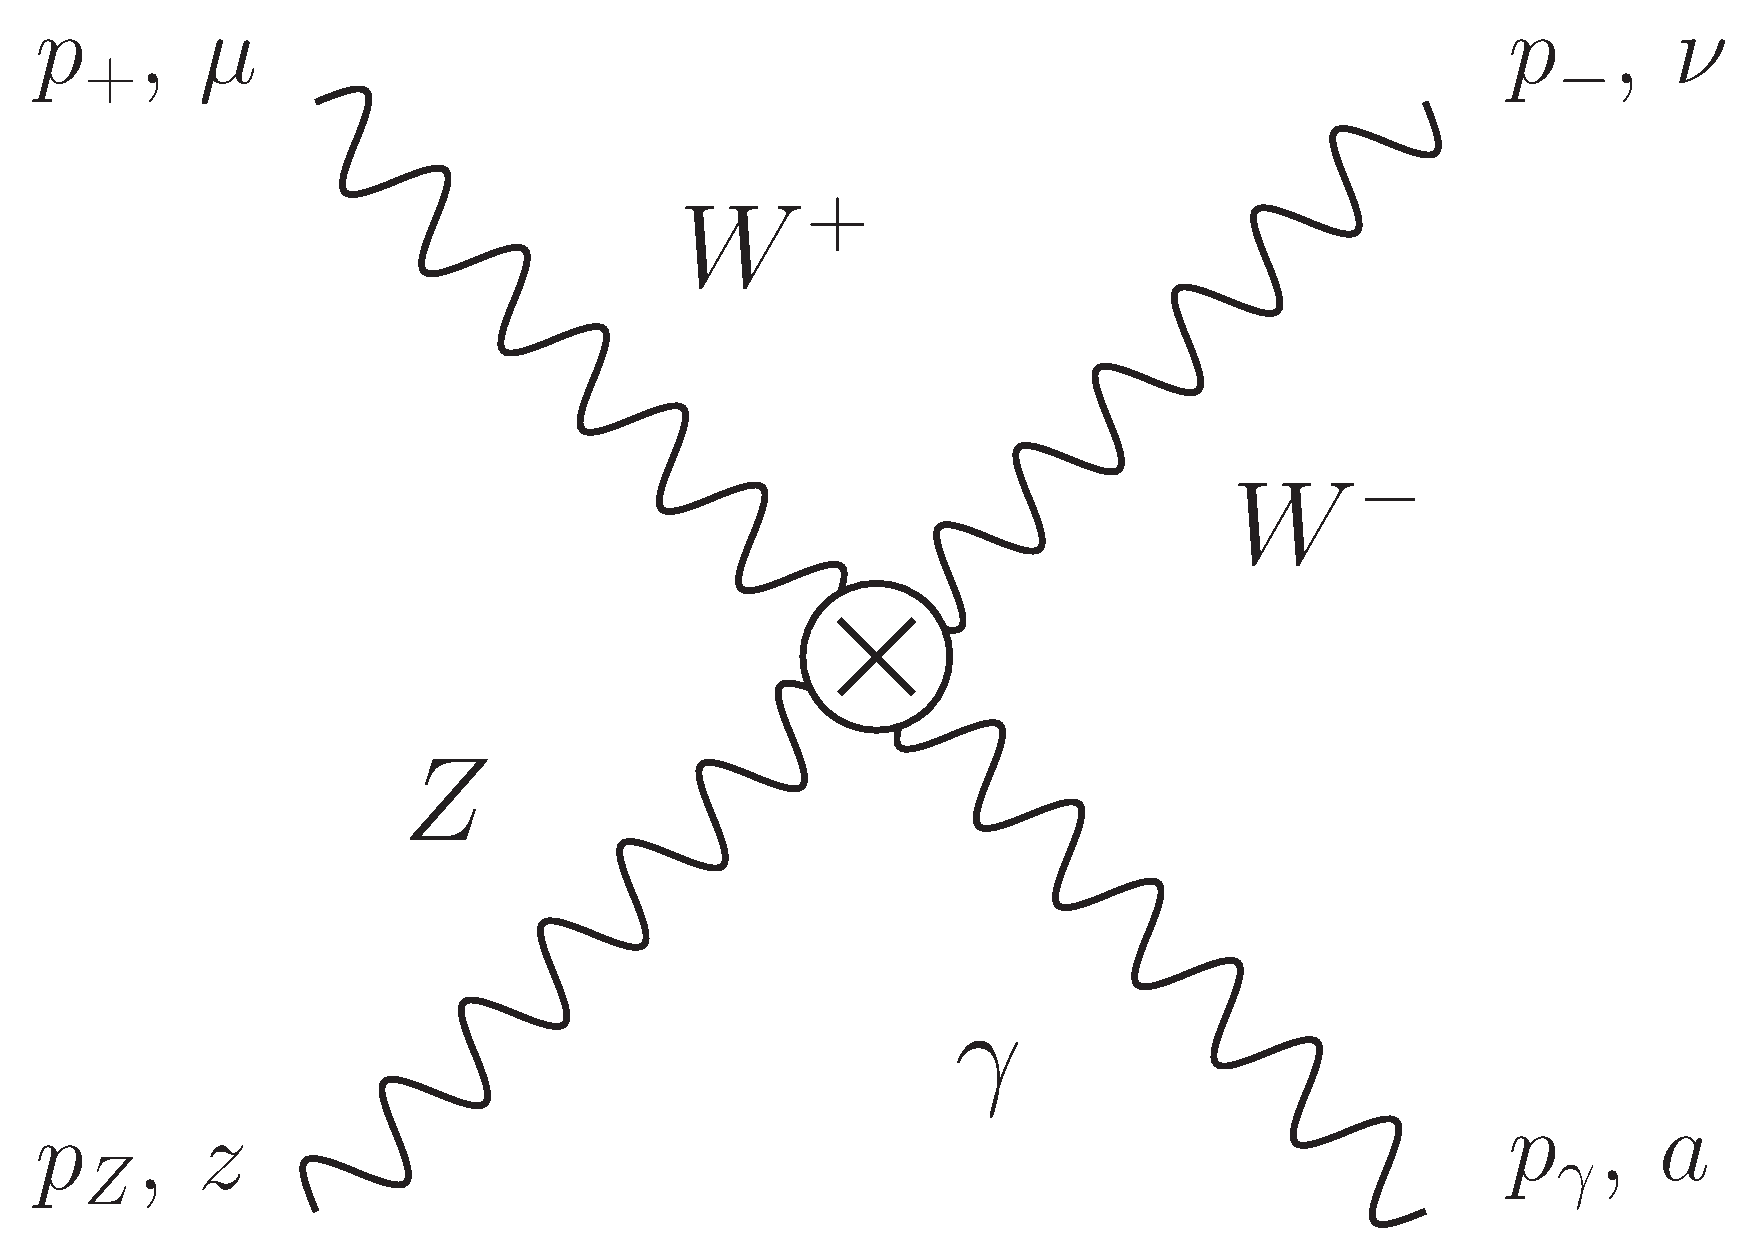
\includegraphics[scale=0.25]{WWZA}
%\end{figure}

%For the vertices $WW\gamma \gamma$ and $WWZ\gamma$, looking at linearly builded dimension 8 operators Eqs. \eqref{dim8_a} and \eqref{dim8_b} and comparing them with Eqs.\eqref{dim8_belanger} together with the relation Eq.\eqref{relation}
%we have
%\begin{eqnarray}
%\dfrac{f_{M2}}{\Lambda^{4}} &=& \dfrac{g^{\prime 2}}{2M_{W}^{4}s^{2}_{W}}\;\dfrac{k_{0}^{b}}{\Lambda^{2}} \nonumber \\
%&& \nonumber\\
%\dfrac{f_{M0}}{\Lambda^{4}} &=& \dfrac{g^{2}}{4M_{W}^{4} s^{2}_{W} }\;\dfrac{k_{0}^{w}}{\Lambda^{2}} \nonumber \\
%&& \nonumber \\
%\dfrac{f_{M4}}{\Lambda^{4}} &=& \dfrac{g\;g^{\prime}}{2M_{W}^{4}s^{2}_{W}}\;\dfrac{k_{0}^{m}}{\Lambda^{2}} \nonumber \\
%&& \nonumber \\
%\dfrac{f_{M3}}{\Lambda^{4}} &=& \dfrac{g^{\prime 2}}{M_{W}^{4}s^{2}_{W}}\;\dfrac{k_{C}^{b}}{\Lambda^{2}}\nonumber \\
%&& \nonumber \\
%\dfrac{f_{M1}}{\Lambda^{4}} &=& \dfrac{g^{2}}{2M_{W}^{4}s^{2}_{W}}\;\dfrac{k_{C}^{w}}{\Lambda^{2}} \nonumber \\
%&& \nonumber \\
%\dfrac{f_{M5}}{\Lambda^{4}} &=& \dfrac{g\;g^{\prime}}{M_{W}^{4}s^{2}_{W}}\;\dfrac{k_{C}^{m}}{\Lambda^{2}}
%\end{eqnarray}

%where $g=e/s_{W}$ and $g^{\prime}=e/c_{W}$.


%In this section, we introduce models we used for our analysis. Instead 
%of studying specific new physics, one can construct an effective 
%Lagrangian in a model-independent way for the anomalous quartic 
%couplings. To build up a resonable model, as a first step, we study the
%lowest possible order operators, which reads 
%6~\cite{500GeVNLC,Belanger:1999}, just as the OPAL group did for LEP 
%analysis ~\cite{wwaLEP:1999,wwaLEP:2004}. In this model, we assume the 
%operators keep $SU(2)_{L} \otimes U(1)_{Y}$ symmetry and $\cal{C}$, 
%$\cal{P}$ independently. In order to fulfill the stringent experimental
%constraint on the $\rho$ parameter, we further require the $SU(2)_C$ 
%custodial symmetry. As for \wwa production, the following structures 
%are included for \wwaa and \wwza 
%interactions~\cite{Belanger:1999,Bosonic:2004PRD}: 

%\begin{center}
%\begin{eqnarray}
% {\cal W}_{0}^{\gamma} = - \frac{e^2 g^2}{2} F_{\mu \nu} F^{\mu \nu} W^{+\alpha} W^{-}_{\alpha} , \\ 

% {\cal W}_{c}^{\gamma} = - \frac{e^2}{16} F_{\mu \nu} F^{\mu \alpha} ( W^{+ \nu} W^{-}_{\alpha} + W^{- \nu} W^{+}_{\alpha} ) , \\

% {\cal W}_{0}^{Z} = - e^2 g^2 F_{\mu \nu} Z^{\mu \nu} W^{+ \alpha} W^{-}_{\alpha} , \\

% {\cal W}_{c}^{Z} = - \frac{e^2 g^2}{2} F_{\mu \nu} Z^{\mu \alpha} ( W^{+ \nu} W^{-}_{\alpha} + W^{- \nu} W^{+}_{\alpha} ) , \\

% {\cal W}_{1}^{Z} = - \frac{e^2 g^2}{2 c_w s_w} F^{\mu \nu} ( W_{\mu \nu}^{+} W_{\alpha}^{-} Z^{\alpha} + W_{\mu \nu}^{-} W_{\alpha}^{+} Z^{\alpha} ) , \\

% {\cal W}_{2}^{Z} = - \frac{e^2 g^2}{2 c_w s_w} F^{\mu \nu} ( W_{\mu \alpha}^{+} W^{- \alpha} Z_{\nu} + W_{\mu \alpha}^{-} W^{+ \alpha} Z_{\nu} ) , \\

% {\cal W}_{3}^{Z} = - \frac{e^2 g^2}{2 c_w s_w} F^{\mu \nu} ( W_{\mu \alpha}^{+} W_{\nu}^{-} Z^{\alpha} + W_{\mu \alpha}^{-} W_{\nu}^{+} Z^{\alpha} ) ,
%\end{eqnarray}
%\end{center}

%where the $e$ is the electromagnetic coupling, $g = e/\sin{\theta_W$}$, 
%$\theta_W$ is the Weinberg angle, and $\Lambda$ is a mass scale 
%characterizing the New Physics. Accordingly, the effective interactions can be expressed by the above 
%operators as

%\begin{center}
%\begin{equation}\label{operator}
%{\cal L}_{0,c} = \frac{k_{0}^{\gamma}}{\Lambda^2} {\cal W}_{0}^{\gamma} + \frac{k_{c}^{\gamma}}{\Lambda^2} {\cal W}_{c}^{\gamma} + \frac{k_{0}^W}{\Lambda^2} {\cal W}_{0}^{Z} + \frac{k_{c}^W}{\Lambda^2} {\cal W}_{c}^{Z} + \sum_{i = 1,2,3} \frac{k_{i}^{W}}{\Lambda^2} {\cal W}_{i}^{Z}, 
%\end{equation}
%\end{center}

%Note the above parametrizations of effective aQGC interactions 
%(Eq.~\ref{operator}) can be realized in both linear and non-linear 
%ways. When no heavy resonance (the Higgs boson in our case) was 
%included, the symmetry can be realized 
%non-linearly~\cite{Bosonic:2004PRD}, while with a Higgs boson in the particle content, the symmetry can be realized 
%linearly ~\cite{Eboli:2006wa}. In the non-linear formalism, there are 
%14 effective photonic operators which respect $SU(2)_C$ custodial 
%symmetry as well as $\cal{C}$ and $\cal{P}$. (See 
%Ref.~\cite{Bosonic:2004PRD}, Eq.~\ref{operator}, where 
%$k_{0,c}^{w,b,m}$, $k_{1,2}^{w,b,m}$, $k_3^{w,m}$ are the coefficients 
%of the relevant 14 terms). Coefficients in Eq~\ref{operator} can be 
%expressed in terms of parameters in this formalism:

%\begin{center}
%\begin{equation}\label{kgamma}
%k_{0,c}^{\gamma} = k_{0,c}^w + k_{0,c}^b + k_{0,c}^m ,
%\end{equation}
%\end{center}

%\begin{center}
%\begin{equation}\label{kW}
%k_{0,c}^W = \frac{c_W}{s_W} k_{0,c}^w - \frac{s_W}{c_W} k_{0,c}^b + c_{ZW} k_{0,c}^m ,
%\end{equation}
%\end{center}

%where $c_{ZW} = \frac{c_W^2 - s_W^2}{2 c_W s_W}$.

%In the context of the our analysis ~\cite{wwaLEP:2004,Royon:2010tw}, 
%the anomalous \wwza contributions were neglected, which can be achieved
%by setting $k_{0,c}^W$ to zero. Considering this constraint, 
%equivalence can be found between the OPAL parameters ($a_{0,c}^W$) and 
%the above ones -- $a_{0,c}^W = 4 g^2 k_{0,c}^{\gamma}$ 
%~\cite{Belanger:1999}. Similar things happen to the linear formalism. 
%As shown in Section 3 of Ref.~\cite{Belanger:1999}, the OPAL operators 
%can be made gauge invariant also in the linear approach and equivalence
%can be found for linear and non-linear parameters:

%\begin{center}
%\begin{equation}
%\frac{Q_{0,c}^{b,w,m}}{\Lambda^2} = \frac{1}{2} \frac{g^2}{M^2_W} k_{0,c}^{b,w,m}
%\end{equation}
%\end{center}

%where $Q_{0,c}^{b,w,m}$ are parameters of the linear formalism.

%Morover, there are more types of QGC operators appearing in the linear 
%formalism which have never been tested before. Therefore, as a second 
%step, we investigate the LT operators in the linear 
%formalism~\cite{Eboli:2006wa}, with new lorentz structures which have 
%never been tested experimentally. 

%\begin{center}
%\begin{eqnarray}\label{operator:LT}
%{\cal L}_{T,0} = Tr[\hat{W}_{\mu \nu} \hat{W}^{\mu \nu}] \times Tr[\hat{W}_{\alpha \beta} \hat{W}^{\alpha \beta}] , \\
%{\cal L}_{T,1} = Tr[\hat{W}_{\alpha \nu} \hat{W}^{\mu \beta}] \times Tr[\hat{W}_{\mu \beta} \hat{W}^{\alpha \nu}] , \\
%{\cal L}_{T,2} = Tr[\hat{W}_{\alpha \mu} \hat{W}^{\mu \beta}] \times Tr[\hat{W}_{\beta \nu} \hat{W}^{\nu \alpha}] .
%\end{eqnarray}
%\end{center}

\subsection{Unitarity and form factor}

The contribution of aQGC operators are strictly prohibited by theory,
since any non-zero value of the aQGCs will lead to tree-level
unitarity violation at sufficiently high energy~\cite{Chapon:2009}. To
dampen the effect of non-unitarity, some people make use of form
factors. However, the choice of form factors is somewhat arbitrary and
subject to dispute, and different choices of form factor make
comparison difficult. So, in our analysis, we present our results
both with and without a form factor.

In order to choose a suitable form factor, one can extract a unitarity
bound from the S-matrix unitarity condition. In
Ref.~\cite{Chapon:2009,AQGC:2001}, the author calculated the unitarity
bound for inelastic photon scattering process. When trying the similar
method for triple gauge boson production processes, one will find that
irrelevant two-to-two processes involved into the calculation, and if we negelect them performing the calculation, the unitarity bound will be much looser than the 2 to 2 ones. At the same time, we should also note
that for any new physics with non-zero values of aQGCs, all related
processes will be affected. Therefore, when analyzing the triple gauge
boson productions, the unitarity bound from two-to-two processes
should also be abided by. Using the unitarity equations in
~\cite{Chapon:2009,AQGC:2001}, we can plot the bound as a function of
center-of-mass energy. Fig ~\ref{aqgc:unitarity} shows that
unitarity is preserved with a choice of form factor of $\Lambda_u
= 500, 600$~GeV in Eq.~\ref{aqgc:ff} when the aQGC $a_0^W/\Lambda^2 = 1
\times 10^{-4}$~GeV$^{-2}$. 

\begin{equation}
 \alpha \rightarrow \frac{\alpha}{(1 + \hat{s}/\Lambda_u^2)^n},
\label{aqgc:ff}
\end{equation}

where the $\alpha$ represent the aQGCs, $\hat{s}$ represent the triple
gauge boson invariant mass, the parameter $\Lambda_{u}$ is a scale
factor that is fixed to 500~GeV, and the parameter n is fixed to 2.

\begin{figure}[]{
\centering
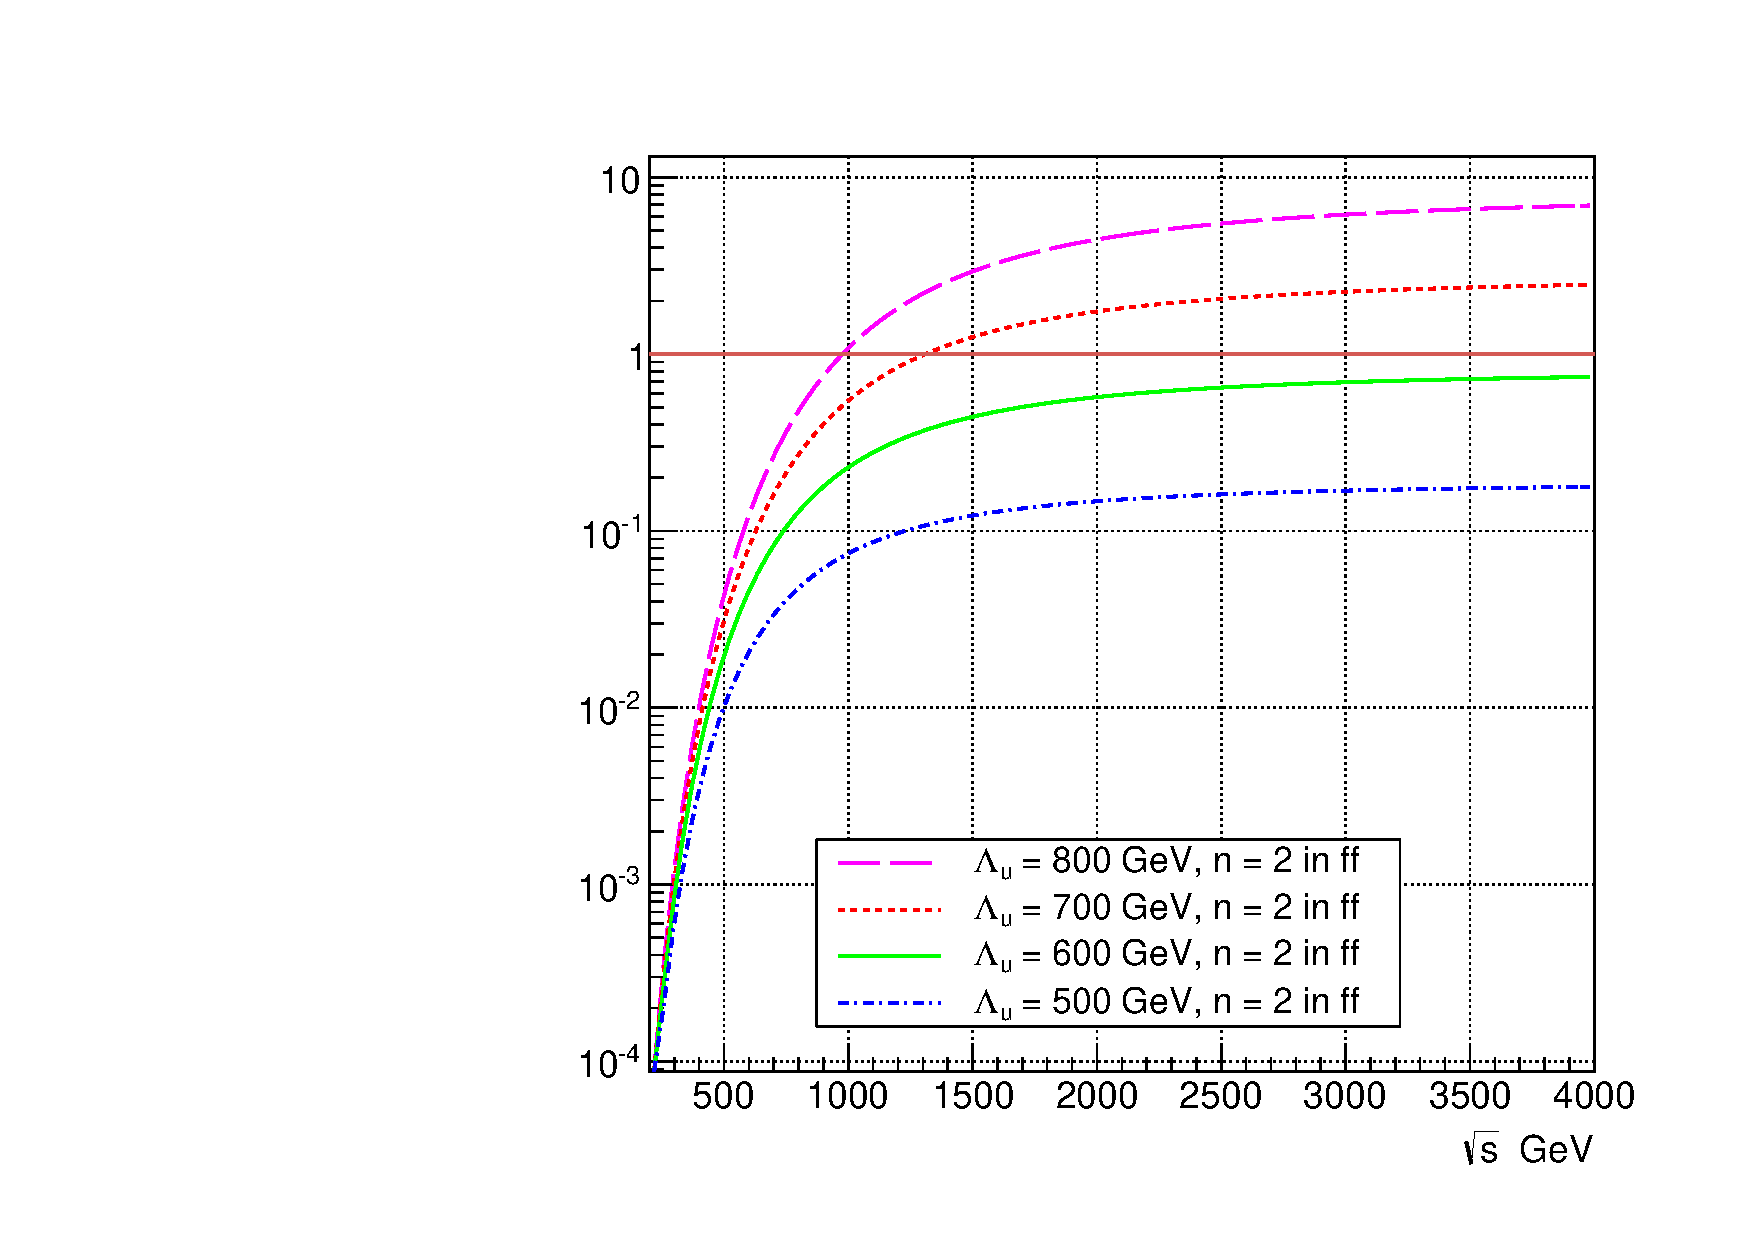
\includegraphics[width=0.4\textwidth]{figs/unitarity.pdf}
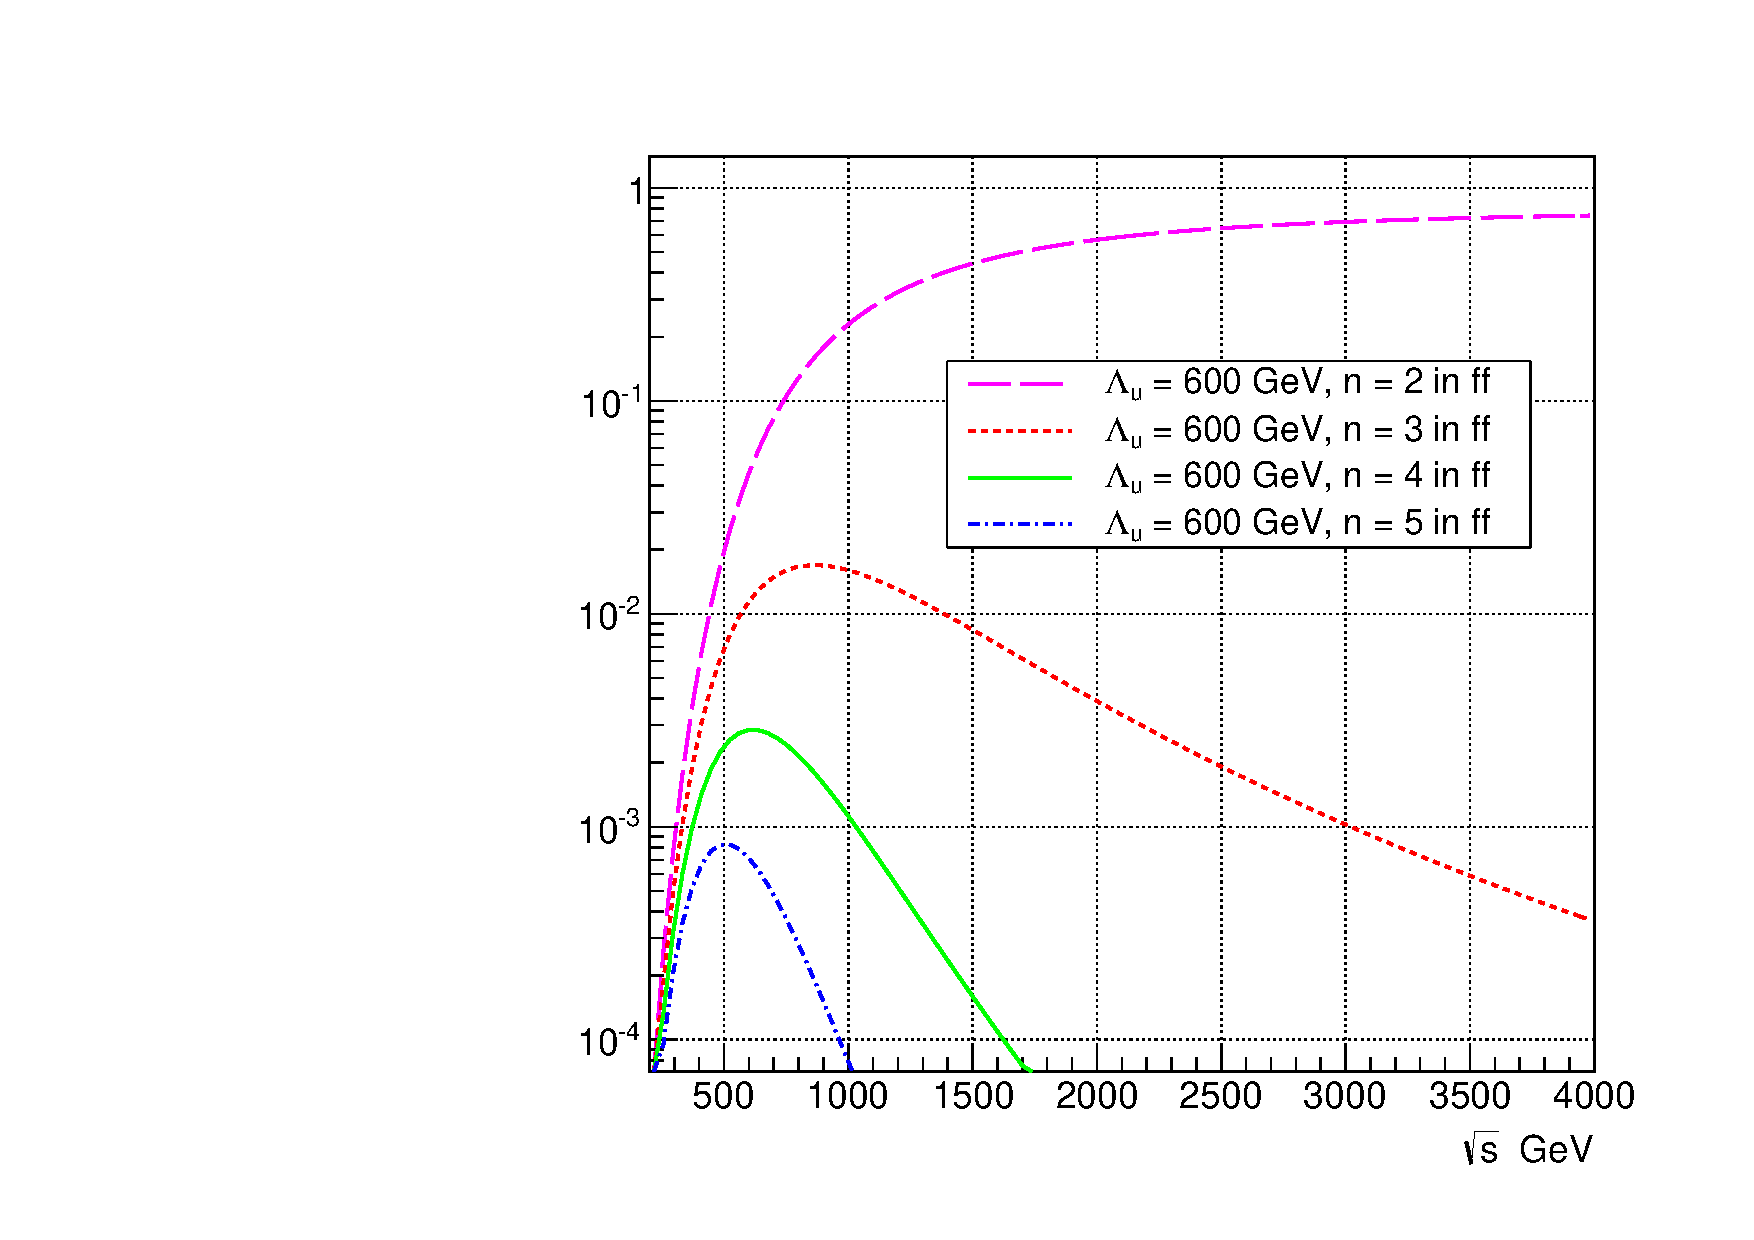
\includegraphics[width=0.4\textwidth]{figs/unitarity_n.pdf}
\caption{\label{aqgc:unitarity} The unitarity condition for aQGC $a_0^W/\Lambda^2 = 1\times 10^{-4}$~GeV$^{-2}$, the unitarity bound is represented by the line of value 1 }}
\end{figure}

We also have examined the unitarity condition for aQGC parameters as a function of the form factor scale $\Lambda_{u}$ and different values of $\hat{s}$, and compared it with the projected
sensitivity of our analysis using 20~\fbinv of integrated luminosity. To do this, we fixed the value of $aQGC \times ff$ to the value of $aQGC$ without a form factor. The center of mass energy dependence is replaced with a fixed effective energy scale representing the typical center of mass energy with non-zero value of a aQGC. In our analysis, we have used the limits with a form factor in Eq.~\ref{aqgc:ff}, which is the same as former CMS analysis on two photon production of W boson pair ~\cite{CMS-PAS-FSQ-12-010}, to fix this effective $\sqrt{\hat{s}}$. In this way, we can vary the value of the effective $\sqrt{\hat{s}}$ to estimate uncertainties of our limits. In Figure ~\ref{aqgc:uniBand} uncertainty bands with 0.5/2, 0.25/4 times the effective $\sqrt{\hat{s}}$ are shown. Besides, we have also drawn theoretical unitarity bound with different $\sqrt{\hat{s}}$ upper limits. The results shown on Figure ~\ref{aqgc:uniBand} indicates that there is no value of the dipole form factor's scale at
which the unitarity condition can be satisfied for all values of
$WW\gamma$ invariant mass, given the available amount of data at
$\sqrt{s}=8$~TeV. This motivates the choice of presenting our results
without any form factor.

\begin{figure}[hb] 
  \begin{center}
    \subfigure[$a_0^W$]{
    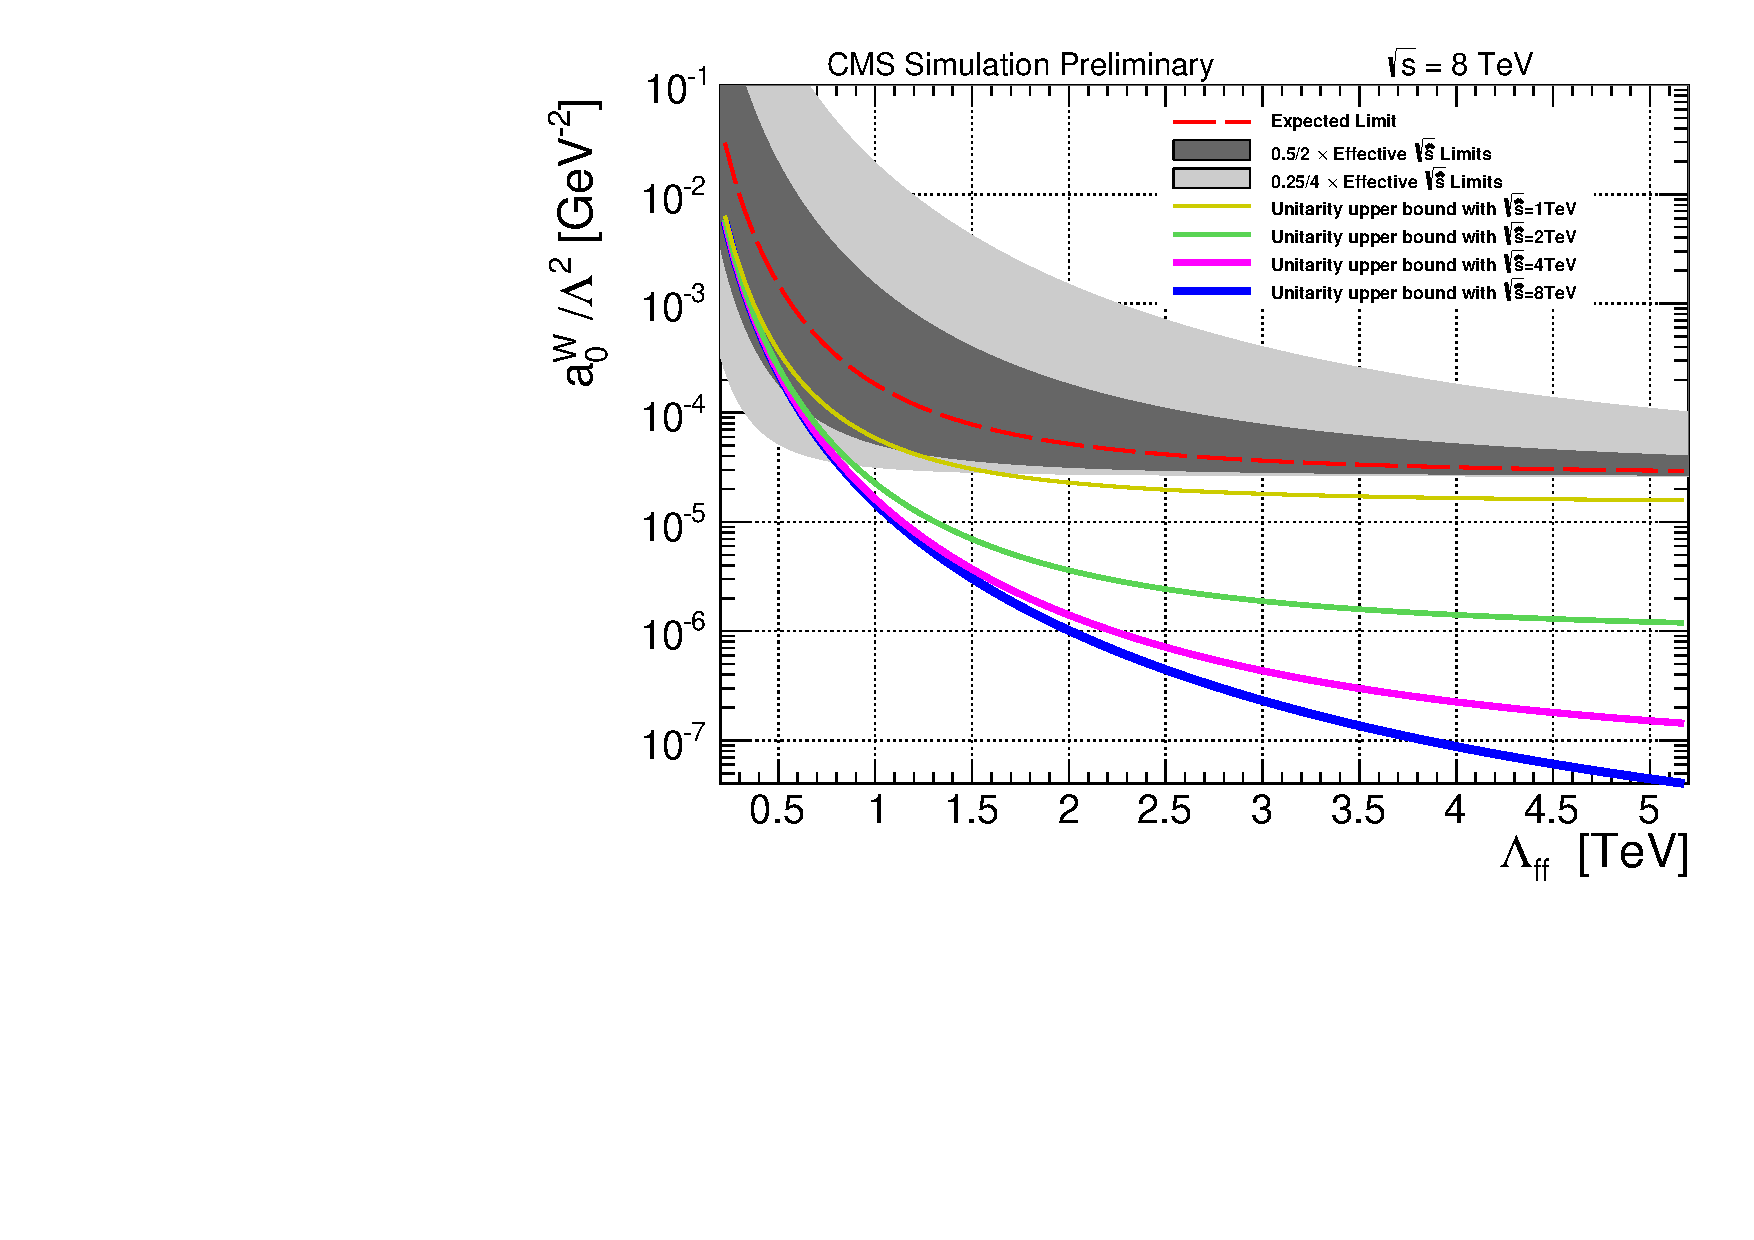
\includegraphics[width=0.48\textwidth]{figs/prounitarity_a0w.pdf}
    }
    \subfigure[$a_C^W$]{
    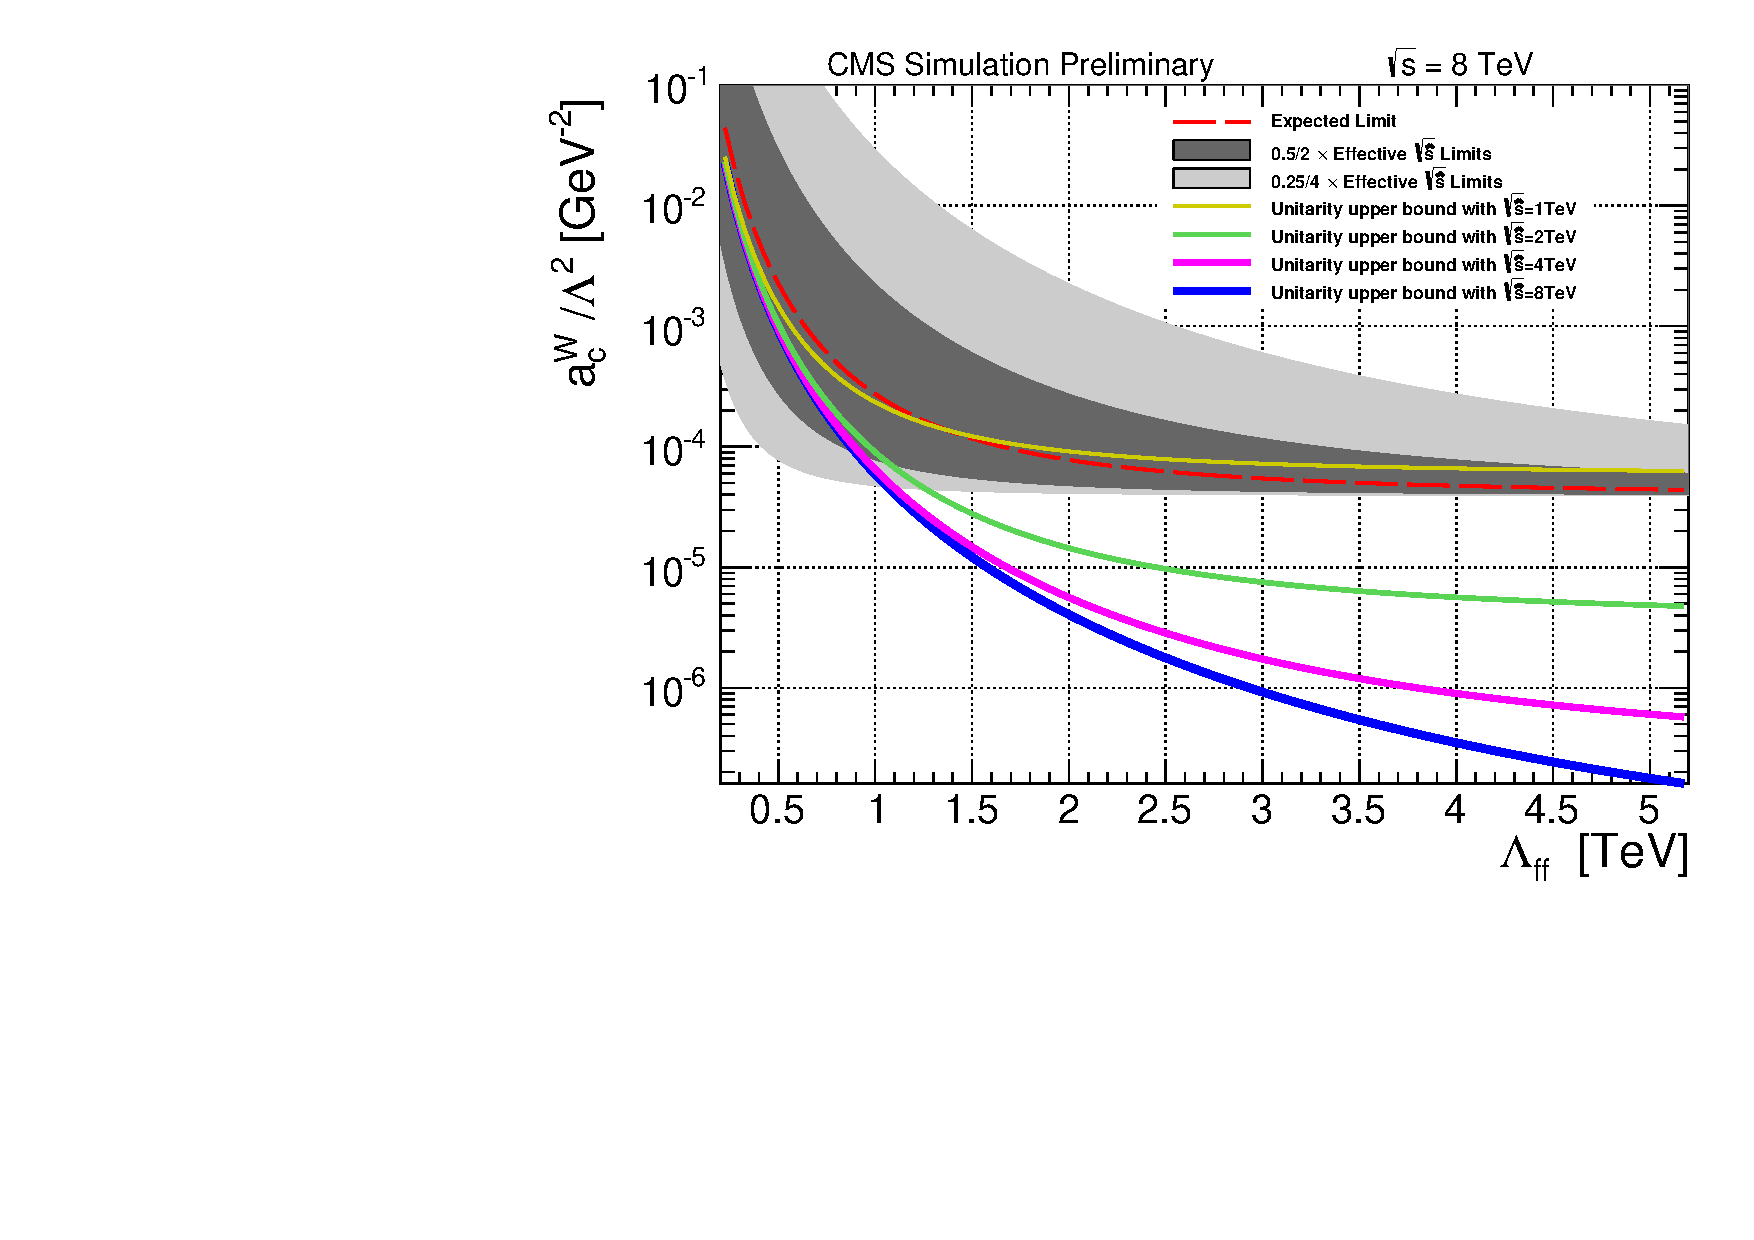
\includegraphics[width=0.48\textwidth]{figs/prounitarity_acw.pdf}
    }\\
    \subfigure[$\kappa_0^W$]{
    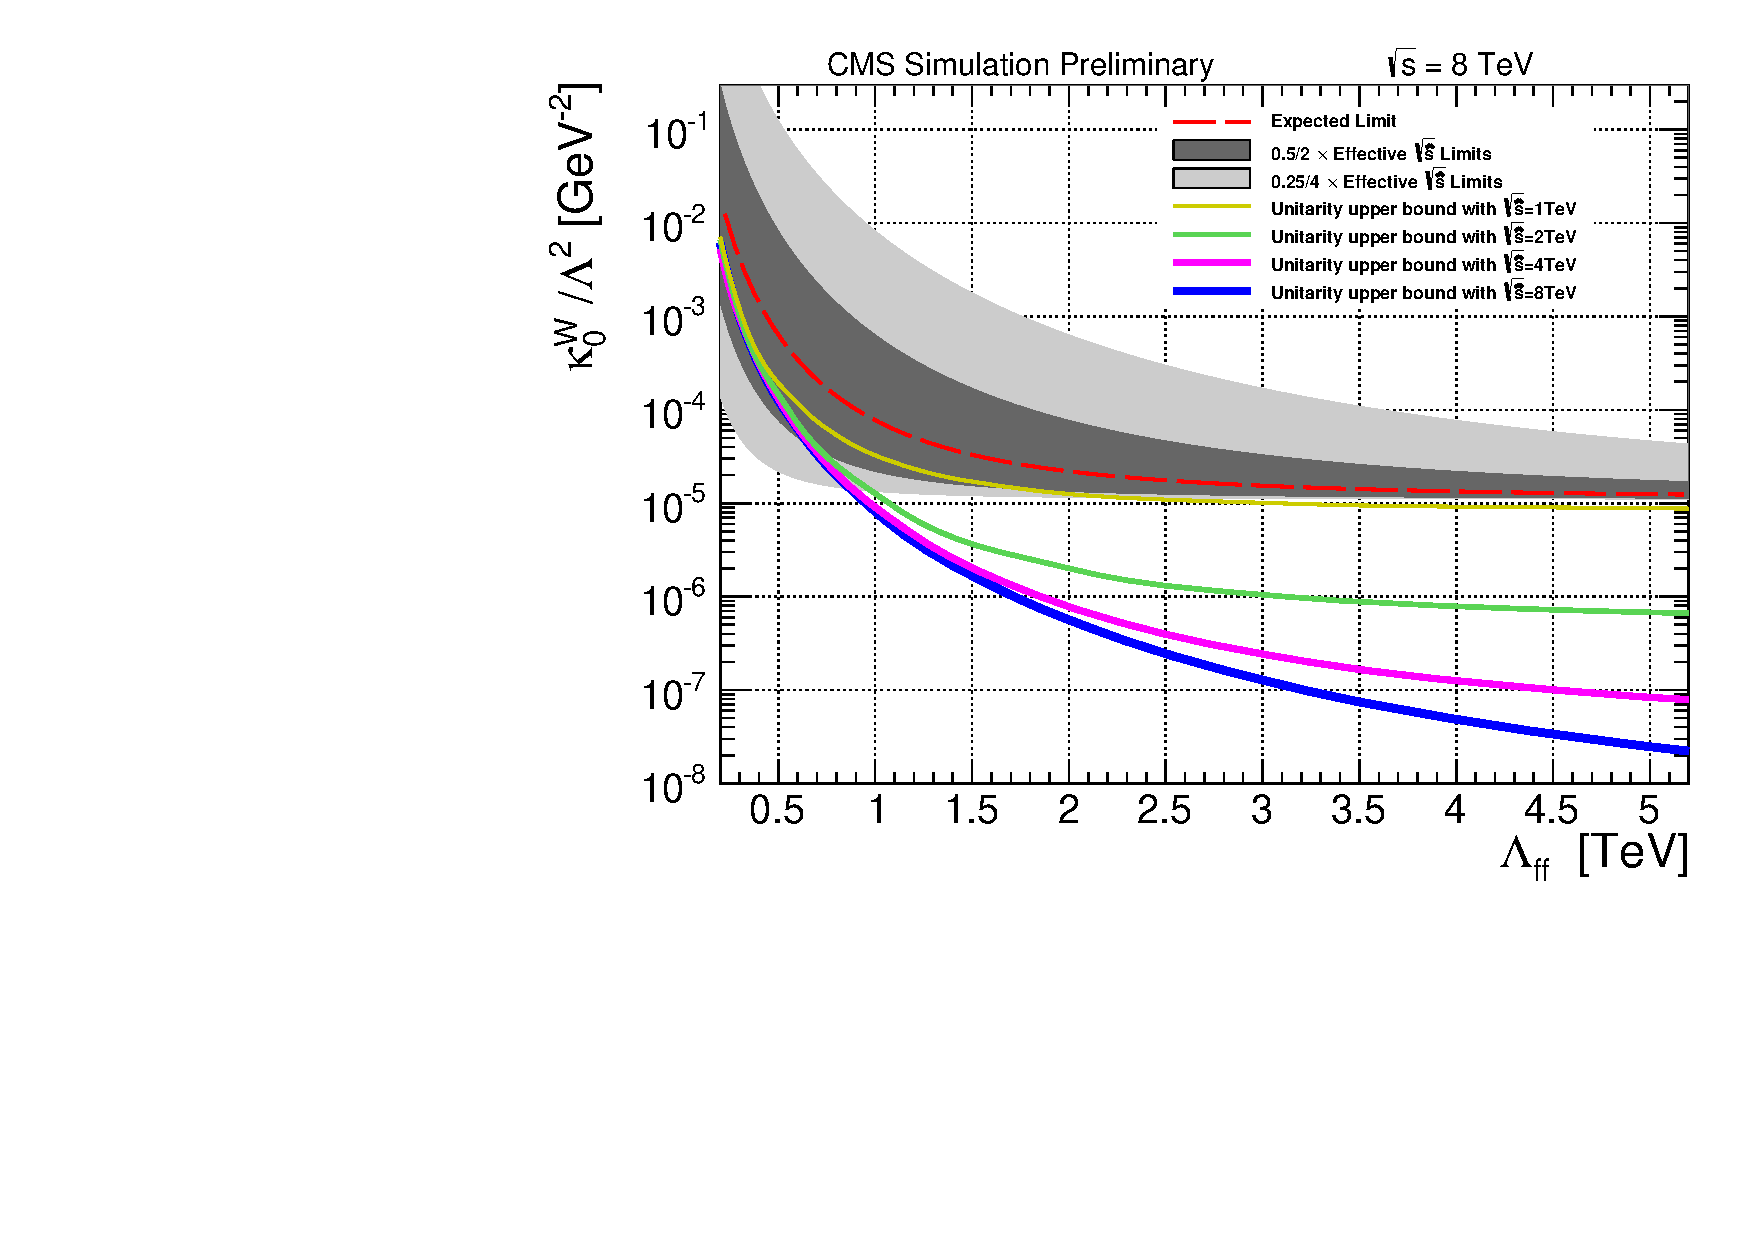
\includegraphics[width=0.48\textwidth]{figs/prounitarity_k0W.pdf}
    }
    \subfigure[$\kappa_C^W$]{
    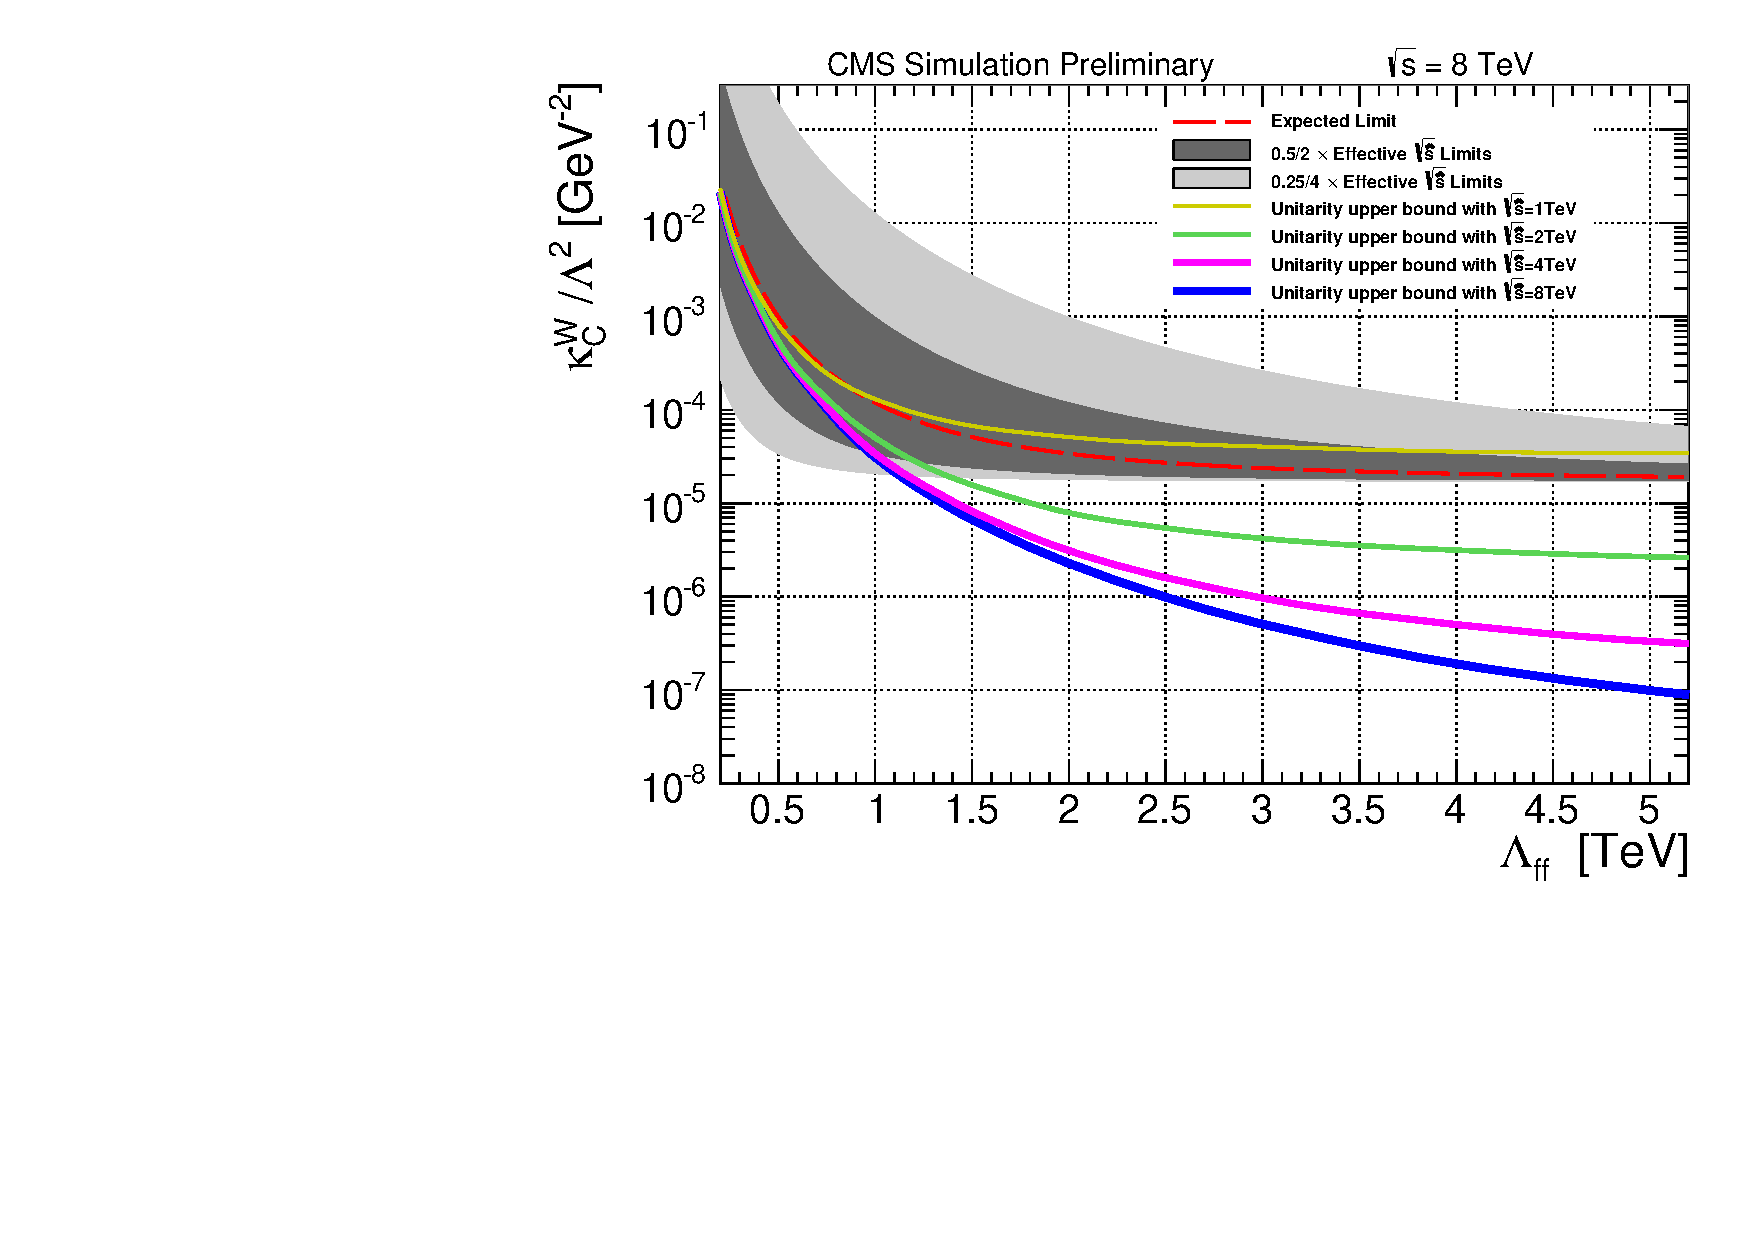
\includegraphics[width=0.48\textwidth]{figs/prounitarity_kCW.pdf}
    }\\
    \subfigure[$f_{T,0}$]{
    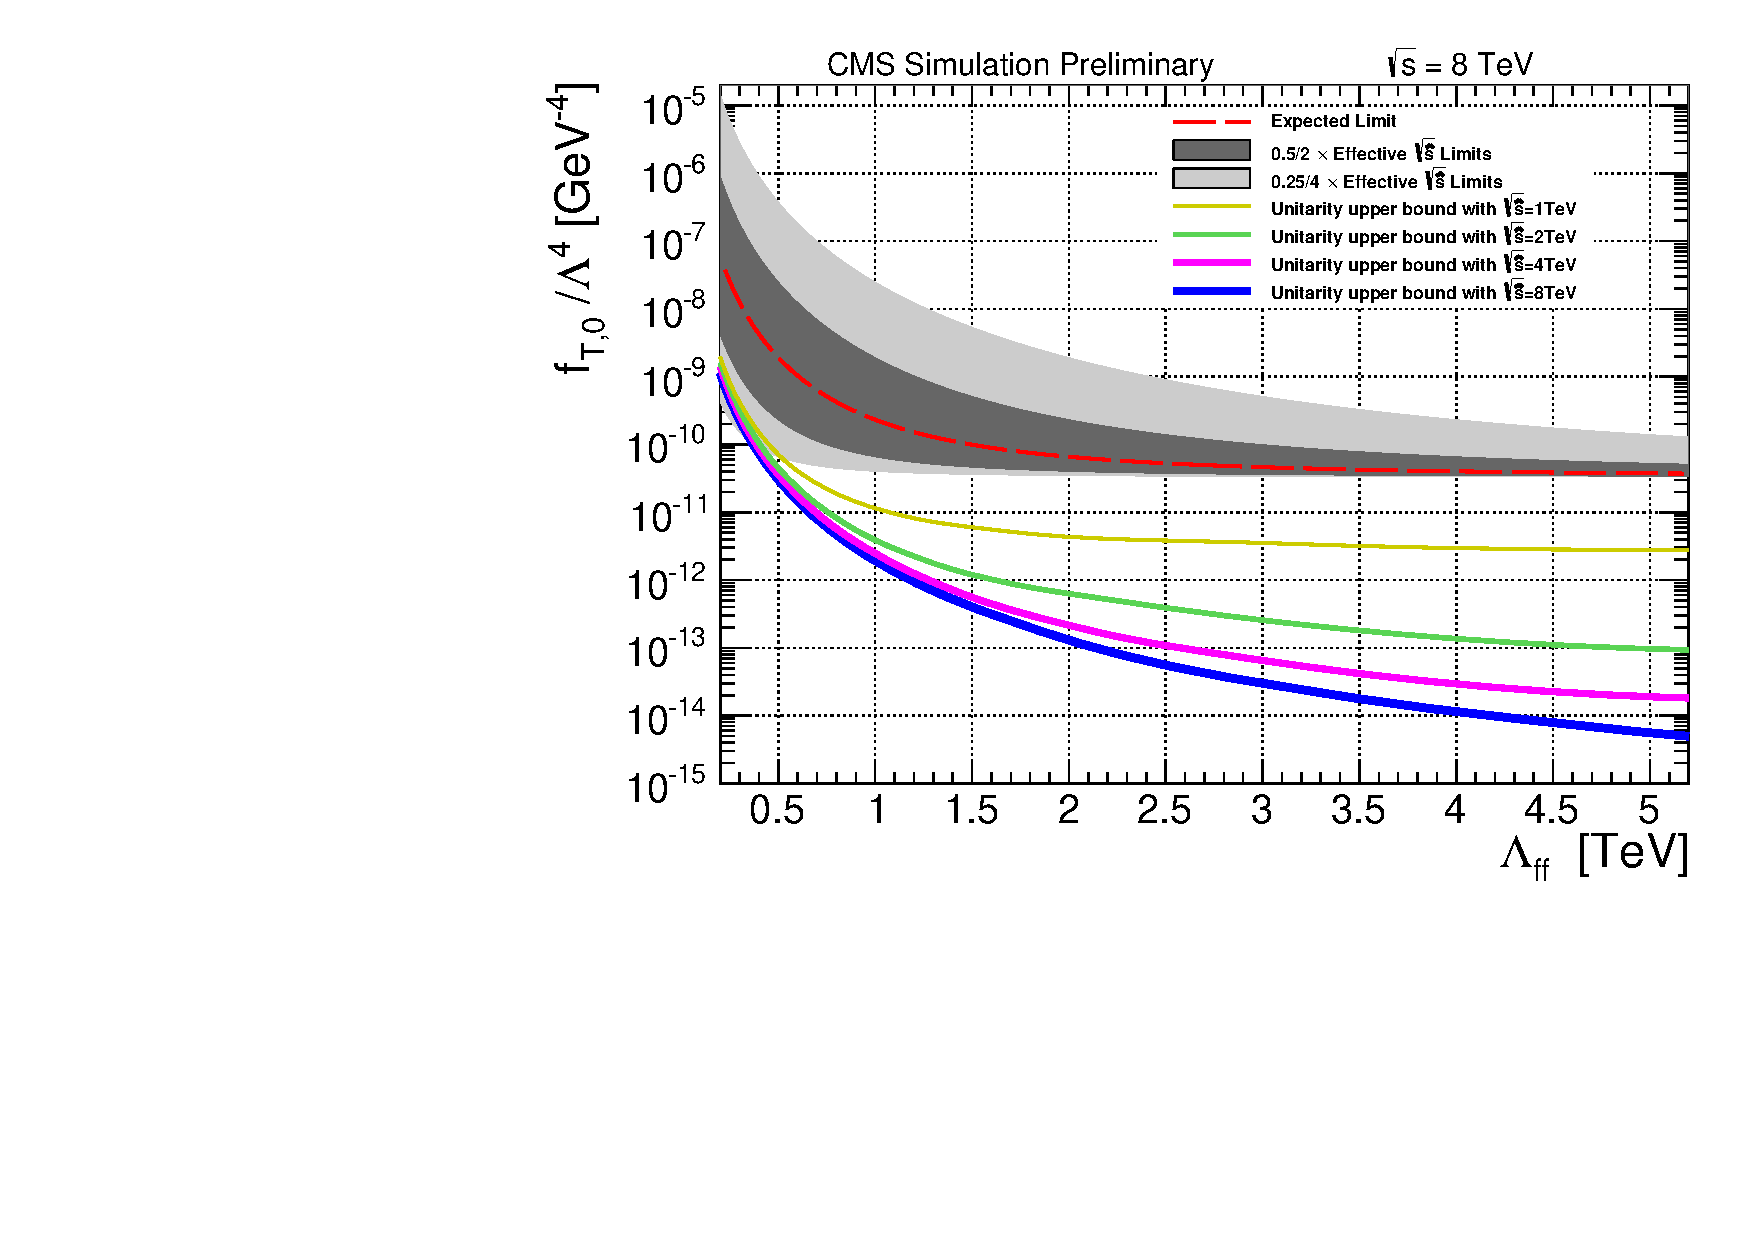
\includegraphics[width=0.48\textwidth]{figs/prounitarity_fT0.pdf}
    }
    \caption{\label{aqgc:uniBand} The unitarity condition for aQGC
    parameters (a) $a_0^W/\Lambda^2$, (b) $a_{C}^{W}/\Lambda^{2}$, (c) $\kappa_0^W/\Lambda^2$, (d) $\kappa_{C}^{W}/\Lambda^{2}$ and
    (e) $f_{T,0}/\Lambda^{4}$ as a function of form factor parameter
    $\Lambda_{u}$ and different values of $\hat{s}$ is compared with
    the projected sensitivity of our analysis using 20~\fbinv of integrated
    luminosity. }
  \end{center}
\end{figure}
\clearpage

\section{Datasets}
\label{sec:technicalities}
% ---- ---- ---- ---- ---- ---- ---- ---- ---- ---- ---- ---- ---- ---- ---- ---- ---- ---- ---- ---- ---- ---- ----

We study $WW\gamma$ and $WZ\gamma$ production in semi-leptonic final state, which has larger branching fraction than the fully leptonic final stat. 
In this final state one $W$ boson decays leptonicaly, while the second W or Z decays hadronicaly. We study those two processes togeter as the di-jet mass resolution of the 
detector doesn't allow them to be cleary separated.  
The larger branching fraction is an advantage when study a rare processes, while the trade off is a higher background rate, which arises from $W\gamma$+jets process. 
This background is the dominant in this channel and resembles approximately 70\% of total oberved rate after the analysis selection. Other contributions arise from processes 
with jets which fake photon (15-20\%), dominaned by W plus three or more jets. The remainig about 10\% of the observed rate is atributed to $t\overline{t}\gamma$ , single 
top, $Z\gamma+jets$, $Z+jets$ and multijets production.  

\subsection{Samples used for the analysis}

The data sample we use in this analysis was recorded by the CMS experiment 
in 2012. The data is collected by single muon ($p_T>23$GeV) and single electron ($p_T>27$GeV) triggers. 
Only certified runs and luminosity sections are considered, which 
means that good functioning of all CMS sub-detectors is required. The total 
statistics analyzed correspond to an integrated luminosity of 19.3~\fbinv.
% \LUMI{}.

The dataset used for the analysis and the corresponding run ranges are 
listed in Table~\ref{tab:datasets}. All samples have been processed using a 
\texttt{CMSSW\_5\_3\_2} release version.

\begin{table}[]
  \begin{center}
  \begin{tabular}{r|r}
  \hline
  Dataset name & Run range \\
  \hline
  /SingleMu/Run2012A-13Jul2012-v1/AOD         & 190456-193621  \\
  /SingleElectron/Run2012A-13Jul2012-v1/AOD   &            \\
  \hline
  /SingleMu/Run2012A-recover-06Aug2012-v1/AOD        &  190782-190949  \\
  /SingleElectron/Run2012A-recover-06Aug2012-v1/AOD  &     \\
  \hline
  /SingleMu/Run2012B-13Jul2012-v1/AOD         &  193833-196531  \\
  /SingleElectron/Run2012B-13Jul2012-v1/AOD   &         \\
  \hline
  /SingleMu/Run2012C-24Aug2012-v1/AOD       & 198022-198913 \\
  /SingleElectron/Run2012C-24Aug2012-v1/AOD & \\
  \hline
  /SingleMu/Run2012C-PromptReco-v2/AOD       & 198934-203746 \\
  /SingleElectron/Run2012C-PromptReco-v2/AOD & \\
  \hline
  /SingleMu/Run2012D-PromptReco-v1/AOD       & 203894-208686 \\
  /SingleElectron/Run2012D-PromptReco-v1/AOD & \\
  \hline
  \hline
  \end{tabular}
  \end{center}
  \caption{Summary of data samples used and run ranges of applicability.}
  \label{tab:datasets}
\end{table}%

\subsection{Monte Carlo samples}

Anomalous quadric gauge coupling samples, as well as samples for a
variety of electroweak and QCD-induced background sources, have been 
generated and showered using different Monte Carlo generators. To better 
reproduce the actual data-taking conditions, where there is a significant 
probability that more than two protons interact in the same bunch crossing,
pile-up (PU) events are added on top of the hard scattering. Particle 
interactions with the detector were reproduced through a detailed 
description of CMS.

The MadGraph5.1.3.22 generator \cite{MadGraph} has been used to produce signal 
events, and the showering has been performed with PYTHIA6 \cite{pythia}. 

The background samples used for the studies are listed in
Table~\ref{tab:MCsamples}.

All MC samples considered in this analysis come from the official
``Summer12\_53X'' or private production.  Events from all samples were
reconstructed making use of a \texttt{CMSSW\_5\_3\_X} release version.
The simulated samples are reweighted to represent the distribution of the
number of pp interactions per bunch crossing (pile-up), as measured in
the data.

\begin{sidewaystable}[htb]
  \begin{center}
  \scalebox{0.8}{
    \begin{tabular}{|c|l|}
      \hline
%%      sample & cross-section (pb) \\
%%      \hline
      $W\gamma+jets$&/WaJets\_lvaJets\_TTU2\_SIM/jdamgov-WAjets\_RECO\_TTU2-6c7dff08e6fc03321df811559605c57f/USER \\
      $W\gamma+jets,p_{T}^{\gamma}>100GeV$ &/WAp23J\_100GeVtail\_8TeV\_CMSSW532\_LHE2EDM/jfaulkne-WApJ\_highPT\_8TeV\_CMSSW532\_RECO-c8f8ed334db8a7d6f56c62266b1dfa5b/USER \\
      $WZ\gamma$&/WZA\_8TeV\_CMSSW532\_LHE2EDM/jfaulkne-WZA\_lvjjA\_8TeV\_CMSSW532\_RECO-c8f8ed334db8a7d6f56c62266b1dfa5b/USER \\
      $Z\gamma+jets$&/ZAp23J\_8TeV\_CMSSW532\_LHE2EDM/jdamgov-ZApJ\_8TeV\_CMSSW532\_RECO-c8f8ed334db8a7d6f56c62266b1dfa5b/USER \\
      $ttbar\gamma+jets$&/TTGJets\_8TeV-madgraph/jdamgov-TTbarAJets\_RECO-c8f8ed334db8a7d6f56c62266b1dfa5b/USER  \\
      $ZZ$&/ZZ\_TuneZ2star\_8TeV\_pythia6\_tauola/Summer12\_DR53X-PU\_S10\_START53\_V7A-v1/AODSIM  \\
      &/T\_t-channel\_TuneZ2star\_8TeV-powheg-tauola/Summer12\_DR53X-PU\_S10\_START53\_V7A-v1/AODSIM \\
      &/T\_s-channel\_TuneZ2star\_8TeV-powheg-tauola/Summer12\_DR53X-PU\_S10\_START53\_V7A-v1/AODSIM \\
      &/T\_tW-channel-DR\_TuneZ2star\_8TeV-powheg-tauola/Summer12\_DR53X-PU\_S10\_START53\_V7A-v1/AODSIM \\
      &/Tbar\_t-channel\_TuneZ2star\_8TeV-powheg-tauola/Summer12\_DR53X-PU\_S10\_START53\_V7A-v1/AODSIM \\
      &/Tbar\_tW-channel-DR\_TuneZ2star\_8TeV-powheg-tauola/Summer12\_DR53X-PU\_S10\_START53\_V7A-v1/AODSIM \\
      &/Tbar\_s-channel\_TuneZ2star\_8TeV-powheg-tauola/Summer12\_DR53X-PU\_S10\_START53\_V7A-v1/AODSIM \\
      \hline
      FT0 -3& /WWA6-LT0m3-MG/qili-WWAAODSIM-c8f8ed334db8a7d6f56c62266b1dfa5b/USER  \\
      FT0 -5& /WWA6-LT0m5-MG/qili-WWAAODSIM-c8f8ed334db8a7d6f56c62266b1dfa5b/USER \\
      FT0 -8& /WWA6-LT0m8-MG/qili-WWAAODSIM-c8f8ed334db8a7d6f56c62266b1dfa5b/USER \\
      FT0 3& /LT0p3\_SIM/dyang-LT0p3\_AODSIM-a14afa9073215900eeee6c01e24940c2/USER \\
      FT0 5& /LT0p05\_SIM/dyang-LT0p5\_AODSIM-a14afa9073215900eeee6c01e24940c2/USER \\
      FT0 8& /LT0p8\_SIM/dyang-LT0p8\_AODSIM-a14afa9073215900eeee6c01e24940c2/USER \\
      \hline
      $a_{C}^{W}$ 3& /WWA6-cm3m5-MG/qili-WWAAODSIM-c8f8ed334db8a7d6f56c62266b1dfa5b/USER \\
      $a_{C}^{W}$ 5& /WWA6-cp5m5-MG/qili-WWAAODSIM-c8f8ed334db8a7d6f56c62266b1dfa5b/USER \\
      $a_{C}^{W}$ 8& /WWA6-cm8m5-MG/qili-WWAAODSIM-2-c8f8ed334db8a7d6f56c62266b1dfa5b/USER \\
      $a_{C}^{W}$ -3& /dim6KCG\_p3m5\_SIM\_v0/zixu-dim6KCG\_p3m5\_SIM\_AODSIM-7d85a48843799f18e4c38abf839f8e2e/USER \\
      $a_{C}^{W}$ -5& /cA6p5m5\_SIM/zixu-cA6p5m5\_AODSIM-7d85a48843799f18e4c38abf839f8e2e/USER \\
      $a_{C}^{W}$ -8& /cA6p8\_SIM/dyang-cA6p8\_2\_AODSIM-a14afa9073215900eeee6c01e24940c2/USER \\
      \hline
      $a_{0}^{W}$ -2&  /WWA6-p2m5-MG/qili-WWA-AODSIM-c8f8ed334db8a7d6f56c62266b1dfa5b/USER \\
      $a_{0}^{W}$ -3&  /WWA6-p3m5-MG/qili-WWA-AODSIM-c8f8ed334db8a7d6f56c62266b1dfa5b/USER \\
      $a_{0}^{W}$ -5&  /WWA6-p5m5-MG/qili-WWAAODSIM-c8f8ed334db8a7d6f56c62266b1dfa5b/USER \\
      $a_{0}^{W}$ 2&  /WWA6-m2m5-MG/qili-WWAAODSIM-c8f8ed334db8a7d6f56c62266b1dfa5b/USER \\
      $a_{0}^{W}$ 3&  /A6m3m5\_SIM/zixu-A6m3m5\_AODSIM-7d85a48843799f18e4c38abf839f8e2e/USER \\
      $a_{0}^{W}$ 5&  /A6m5m5\_SIM/zixu-A6m5m5\_AODSIM-7d85a48843799f18e4c38abf839f8e2e/USER \\
      \hline
      $\kappa_{0}^{W}$ -2& /aWWA\_k0W\_m2\_8TeV\_CMSSW532\_GEN/jfaulkne-aWWA\_k0W\_m2\_8TeV\_CMSSW532\_RECO-c8f8ed334db8a7d6f56c62266b1dfa5b/USER  \\
      $\kappa_{0}^{W}$ -1& /aWWA\_K0W\_m1\_8TeV\_CMSSW532\_LHE2EDM/jfaulkne-aWWA\_k0W\_m1\_8TeV\_CMSSW532\_RECO-c8f8ed334db8a7d6f56c62266b1dfa5b/USER   \\
      $\kappa_{0}^{W}$ -0.5& /aWWA\_k0W\_m05\_8TeV\_CMSSW532\_GEN/jfaulkne-aWWA\_k0W\_m05\_8TeV\_CMSSW532\_RECO-c8f8ed334db8a7d6f56c62266b1dfa5b/USER    \\
      $\kappa_{0}^{W}$ 0.5& /aWWA\_k0W\_p05\_8TeV\_CMSSW532\_GEN/jfaulkne-aWWA\_k0W\_p05\_8TeV\_CMSSW532\_RECO-c8f8ed334db8a7d6f56c62266b1dfa5b/USER   \\
      $\kappa_{0}^{W}$ 1& /aWWA\_k0W\_p1\_8TeV\_CMSSW532\_GEN/jdamgov-SQWaT\_PAT\_53X\_Summer12\_k0Wp1-829f288d768dd564418efaaf3a8ab9aa/USER  \\
      $\kappa_{0}^{W}$ 2& /aWWA\_K0W\_p2\_8TeV\_CMSSW532\_LHE2EDM/jfaulkne-aWWA\_k0W\_p2\_8TeV\_CMSSW532\_RECO-c8f8ed334db8a7d6f56c62266b1dfa5b/USER   \\
      \hline
      $\kappa_{C}^{W}$ -3& /aWWA\_kCW\_m3\_8TeV\_CMSSW532\_GEN\_TTU/jdamgov-SQWaT\_PAT\_kCWm3\_8TeV\_WWZA-829f288d768dd564418efaaf3a8ab9aa/USER \\
      $\kappa_{C}^{W}$ -2& /aWWA\_kCW\_m2\_8TeV\_CMSSW532\_GEN\_TTU/jdamgov-SQWaT\_PAT\_kCWm2\_8TeV\_WWZA-829f288d768dd564418efaaf3a8ab9aa/USER \\
      $\kappa_{C}^{W}$ -1& /aWWA\_kCW\_m1\_8TeV\_CMSSW532\_GEN\_TTU/jdamgov-SQWaT\_PAT\_kCWm1\_8TeV\_WWZA-829f288d768dd564418efaaf3a8ab9aa/USER \\
      $\kappa_{C}^{W}$ 1& /aWWA\_kCW\_p1\_8TeV\_CMSSW532\_GEN/prebello-SQWaT\_PAT\_kCWp1\_8TeV-829f288d768dd564418efaaf3a8ab9aa/USER \\
      $\kappa_{C}^{W}$ 3& /aWWA\_kCW\_p3\_8TeV\_CMSSW532\_GEN/prebello-SQWaT\_PAT\_kCWp3\_8TeV-829f288d768dd564418efaaf3a8ab9aa/USER \\
      \hline
    \end{tabular}
  }
  \end{center}
  \caption{Summary of Monte Carlo samples used in the analysis.}
  \label{tab:MCsamples}
\end{sidewaystable}

A summary of the cross section of the contributing processes is given in Table ~\ref{tab:samples}

\begin{table}[htb]
\centering
\scalebox{1.15}{
  \begin{tabular}{|c|c|c|}
  \hline
  Process & shape modeling & cross section [pb] \\
  \hline
  \hline
  SM WW$\gamma$                  & MC           & (NLO)      0.0582 $\pm$ 0.0138    \\
  SM WZ$\gamma$                  & MC           & (NLO)      0.0121 $\pm$ 0.0029    \\
  W$\gamma$+Jets                 & MC           & (data)    10.872  $\pm$ 0.087    \\
  jet$\rightarrow\gamma$         & data         &  data                 \\
  Z$\gamma$+Jets                 & MC           & (LO)       0.632   $\pm$ 0.126 \\
  t$\overline{t}\gamma$          & MC           & (LO)       0.615   $\pm$ 0.123 \\
  Single Top + $\gamma$(inclusive)& MC           & (NLO)    0.310     $\pm$ 0.011  \\
  \hline
  \end{tabular}}
  \caption{Summary of the SM processes.Photon \pt $>$ 10 GeV, $|\eta^{\gamma}|<2.5$. }
  \label{tab:samples}
\end{table}


%%%%%%%%%%%%%%%%%%%%%%%%%%%%%%%%%%%%%%%%%%%%%%%%%%%%%%%%%%%%%%%%%%%%%%%%%%
%%%%%%%%%%%%%%%%%%%%%%%%%%%%%%%%%%%%%%%%%%%%%%%%%%%%%%%%%%%%%%%%%%%%%%%%%%
\clearpage{}
\section{Physics objects reconstruction}
\label{sec:reco}
\label{sec:firstStep}
% ---- ---- ---- ---- ---- ---- ---- ---- ---- ---- ---- ---- ---- ---- ----
The study of the $WV\gamma$ final state involves reconstruction of variety of physics object - electrons, muons missing transverse energy, jets and photons. 
In this section we describe in details the all physics objects involved in the analysis. 


The analysis relies on the standard reconstruction algorithms
produced by the CMS community. Event data is reconstructed using the 
particle-flow (PF) reconstruction technique~\cite{pflow}. Particle flow 
attempts to reconstruct all stable particles in an event by combining 
information from all sub-detectors. The algorithm categorizes all particles 
into the following five types: muons, electrons, photons, charged and 
neutral hadrons. The list of reconstructed particles is used as the set of
inputs for a jet clustering algorithm to create particle-flow jets.
%%%%%%%%%%%%%%%%%%%%%%%%%%%%
\subsection{Electron selection}
\label{sec:electron_cuts}

Electrons are reconstructed using a gaussian-sum filter (GSF)
algorithm \cite{CMS-PAS-EGM-10-004}, and are required to pass electron
ID cuts according to a multi-variate identification
technique~\cite{cite:elemva}.  We also require that selected
electron candidates are isolated. Particle flow-based relative
isolation is defined as
%%%
\begin{equation*}
\mathrm{RelIso_{\mathrm{PF}}} = \frac{I_{\mathrm{CH}}+max(0,I_{\mathrm{NH}}+I_{\mathrm{PHOTON}}-(\mathrm{EA}\cdot\rho))}{E_\mathrm{T}},
\end{equation*}
%%%
where $I_{\mathrm{CH}}$, $I_{\mathrm{NH}}$ and $I_{\mathrm{PHOTON}}$
are the charged hadron, neutral hadron and photon isolation variables
(using an isolation cone of 0.3). The $I_{\mathrm{CH}}$ variable is calculated from charged hadrons, associated to the primary vertex.
The neutral hadron and photon isolation variables are corrected for
contributions from pile-up using the effective area correction \cite{EAcorrElectrons},
$(\mathrm{EA}\cdot\rho)$, where $\mathrm{EA}$ is the cone effective area
and $\rho$ is the average neutral particle density of the event.

The ID and isolation cuts used are shown in Table~\ref{tab:EleID} and
have been tuned by Egamma POG to give the same efficiency bin-by-bin with respect to
the working point (WP) used for 2011 analysis.

Additionally, we require
%%%%%%%%%%%%%%%%%%%
\begin{itemize}
\item Electron $E_\mathrm{T} > 30\,\mathrm{GeV}$.
\item Pseudorapidity $|\eta| < 2.5$. There is an exclusion range due
        to the ECAL barrel-endcap transition region, defined by
        $1.4442 < |\eta_{\mathrm{sc}}| < 1.566$, where
        $\eta_{\mathrm{sc}}$ is the pseudorapidity of the ECAL
        supercluster.
%\item Impact parameter: We cut on the absolute value of the impact
%       parameter calculated with respect to the average primary vertex (PV). We
%       require: $d_0(\mathrm{PV}) < 0.02\,\mathrm{cm}.$

%\item In order to make sure that the selected electron and the selected
%jets come from the same hard interaction and not from pile up events,
%we require that the $z$ coordinate of the PV of the event and the $z$
%coordinate of the electron's vertex lie within a distance of
%less than $0.1~\mathrm{cm}$.


\item
In order to reject events in which the electron candidate actually
originates from a conversion of a photon into an $e^{+}e^{-}$ pair, we
use an approach using the vertex fit probability of fully
reconstructed conversions combined with the requirement that the
number of missed inner tracker layers of the electron track must be
exactly zero (i.e. there are no missed layers before the first hit of
the electron track from the beam line).
\end{itemize}

\begin{table}[bthp]
\begin{center}
{\footnotesize
\begin{tabular}{|c|c|c|c|}
\hline
Lepton $\eta$ & $|\eta| < 0.8$ & $0.8 < |\eta| < 1.479$ & $1.479 < |\eta| < 2.5$  \\
\hline
ID MVA cut value (tight lepton) & 0.913 & 0.964 & 0.899 \\
Isolation cut value (tight lepton) & 0.105 & 0.178 & 0.150 \\
ID MVA cut value (loose lepton) & 0.877 & 0.811 & 0.707 \\
Isolation cut value (loose lepton) & 0.426 & 0.481 & 0.390 \\
\hline
\end{tabular}
\caption[.]{\label{tab:EleID} Cut values for electron identification
MVA output and for isolation which are tuned to give the same
efficiency as VBTF Working Point (WP) 80, as used for the tight
electron selection, and VBTF Working Point (WP) 90, as used in the
loose electron selection.}}
\end{center}
\end{table}


%%%%%%%%%%%%%%%%%%%
%%%%%%%%%%%%%%%%%%%%%%%%%%%%%%%%%%%%%%%%%%%%%%%%%%%%%%%%%%%%%%%%%%%%%%%%%%%%
%%%%%%%%%%%%%%%%%%%%%%%%%%%%%%%%%%%%%%%%%%%%%%%%%%%%%%%%%%%%%%%%%%%%%%%%%%%%
\subsection{Muon selection}
\label{sec:muon_cuts}

Muon candidates are identified by two different
algorithms~\cite{MUONPAS}: one proceeds from the inner tracker outwards,
the other one starts from tracks measured in the muon chambers and matches
and combines them with tracks reconstructed in the inner tracker.
These selection criteria\cite{muonIDtwiki} are summarized below:
%%%%%%%%%%%%%%%%%%%
\begin{itemize}
\item The muon candidate is reconstructed both as a global muon and
as a tracker muon.
\item Number of pixel hits of the Tracker track $\ge 1$;
\item Number of muon system hits of the Global track $\ge 1$;
\item Normalized $\chi^{2}$ of the Global track $< 10.0$.
\item Muon $p_{\mathrm{T}} > 25\,\mathrm{GeV}$.
\item Pseudorapidity $|\eta| < 2.1$.
\item Impact parameter: We cut on the absolute value of the impact
parameter calculated with respect to the primary vertex. We require:
$d_0(\mathrm{PV}) < 0.02\,\mathrm{cm}.$
\item In order to make sure that the selected muon and the selected
jets come from the same hard interaction and not from pile up events,
we require that the $z$ coordinate of the PV of the event and the $z$
coordinate of the muon's inner track vertex lie within a distance of
less than 0.5~cm.
\item The number of tracker layers with hits from the muon track has to be
$N_{\mathrm{layers}} > 5$.
\end{itemize}

The selected muon candidates also have to be isolated. Particle
flow-based relative isolation for muons is defined as
\begin{equation*}
\mathrm{RelIso_{\mathrm{PF}}} = \frac{I_{\mathrm{CH}}+max(0,I_{\mathrm{NH}}+I_{\mathrm{PHOTON}}-(0.5~{p}_{T}^\mathrm{sumPU}))}{p_\mathrm{T}},
\end{equation*}

where $I_{\mathrm{CH}}$, $I_{\mathrm{NH}}$ and $I_{\mathrm{PHOTON}}$
are the charged hadron, neutral hadron and photon isolation variables
(using an isolation cone of 0.4). The charged hadron isolation variable uses tracks from the primary vertices only. 
The neutral hadron and photon isolation variables are corrected for
contributions from pile-up using the DeltaBeta correction, $(0.5
p_T^\mathrm{sumPU})$. We require the muon to have
$\mathrm{RelIso_{\mathrm{PF}}} < 0.12$ in order to be considered
isolated.


\subsubsection{Loose Electron}
For the purposes of rejecting events with more than one lepton we
define a loose electron, which has looser cuts. We consider electrons
which have $p_{\mathrm{T}} > 20\,\mathrm{GeV}/c$, $|\eta| < 2.5$,
and which satisfy electron $\mathrm{RelIso_{\mathrm{PF}}}$ and MVA ID
cuts. The cut values for the electron ID and isolation used in the
analysis can be found in Table~\ref{tab:EleID}.
%As in the case of the
%tight electrons, we also require $d_0(\mathrm{PV}) <
%0.02\,\mathrm{cm}$ and that the $z$ coordinate of the PV of the event
%and the $z$ coordinate of the electron's vertex lie within a distance
%of less than $0.1~\mathrm{cm}$.

\subsubsection{Loose Muon}
Additionally, to reject events with more than one lepton, we define a
loose muon, which has looser cuts. We consider all global muons which
have $p_{\mathrm{T}} > 10\,\mathrm{GeV}/c$, $|\eta| < 2.5$, and
$\mathrm{RelIso_{\mathrm{PF}}} < 0.2$ to be loose muons.

%%%%%%%%%%%%%%%%%%%%%%%%%%%%%%%%%%%%%%%%%%%%%%%%%%%%%%%%%%%%%%%%%%%%%%%%%%%%
%%%%%%%%%%%%%%%%%%%%%%%%%%%%%%%%%%%%%%%%%%%%%%%%%%%%%%%%%%%%%%%%%%%%%%%%%%%%
%%%%%%%%%%%%%%%%%%%%%%%%%%%%%%%%%%%%%%%%%%%%%%%%%%%%%%%%%%%%%%%%%%%%%%%%%%%%
%%%%%%%%%%%%%%%%%%%%%%%%%%%%%%%%%%%%%%%%%%%%%%%%%%%%%%%%%%%%%%%%%%%%%%%%%%%%
\subsection{Jet selection}
\label{sec:firstStep_jets}
Jets are reconstructed with the anti-KT algorithm \cite{cacciari},
starting from the set of objects reconstructed by the particle
flow \cite{pflow,CMS-PAS-JME-10-003,CMS-PAS-PFT-10-002}.
Jets are corrected such that the measured energy of the jet
correctly reproduces the energy of the initial particle.
The CMS standard L2 (relative) correction makes the jet response flat in $\eta$.
The standard L3 (absolute) correction brings the jet closer to the $\PT$ of
a matched generated jet created using generator level input and a similar
jet clustering algorithm.
The L2 and L3 corrections are calculated using Monte Carlo, and thus a
L2L3 residual correction is applied that fixes the discrepancies between
Monte Carlo and data~\cite{newjes-cms}.
In this analysis we use jets with measured (corrected) $\PT$
greater than 30~$\gev$.
We require $|\eta| < 2.4$ so that the jets fall within the
tracker acceptance.  Jets from pile-up are identified and removed with PileupJetID tool ~\cite{cite:PileupJetID}.

Jets are required to pass a set of loose identification
criteria; this requirement eliminates jets originating from or being seeded by
noisy channels in the calorimeter~\cite{Chatrchyan:2009hy}:

%%%%%%%%%%%%%%
\begin{itemize}
\item Fraction of energy due to neutral hadrons $<$ 0.99.
\item Fraction of energy due to neutral EM deposits $<$ 0.99.
\item Number of constituents $>$ 1.
\item Number of charged hadrons candidates $>$ 0.
\item Fraction of energy due to charged hadrons candidates $>$ 0.
\item Fraction of energy due to charged EM deposits $<$ 0.99.
\end{itemize}
%%%%%%%%%%
All energy fractions are calculated from uncorrected jets.

\par
In order to account for electron and muon objects that
have been reconstructed as jets, we remove from the jet
collection any jet that falls within a
cone of radius $R= 0.3$ of a loose electron or a loose muon.
This ``cleaning'' procedure is applied in order to ensure that the same
particle is not double counted as two different physics objects.

%%%%%%%%%%%%%%%%%%%%%%%%%%%%%%%%%%%%%%%%%%%%%%%%%%%%%%
%%%%%%%%%%%%%%%%%%%%%%%%%%%%%%%%%%%%%%%%%%%%%%%%%%%%%%
\subsection{Missing Transverse Energy (\MET)}
\label{sec:MET}
An accurate \MET measurement is essential for distinguishing
the $\Wo$ signal from QCD backgrounds.
We use the \MET estimate provided by the Particle Flow algorithm.
PF \MET showed the best performance
among several \MET algorithms~\cite{PFMET}.
The \MET is computed as the vector sum of all PF objects.
It has energy scale correction (type 1) and also "shift" correction, which account for small misalignment of various sub-detector systems.
A good agreement is found between the \MET
distributions of $\Wln$ events in data and simulation~\cite{metPAS}.
The resolution for inclusive multi-jet samples and for
$\Wln$ events is also well reproduced by the simulation.
A relative broadening of a few percent is observed in the data compared to MC,
and has a negligible impact on the
extraction of the W yields~\cite{WZCMS:2010}.
We reject events with small opening angle between \MET and any of the two leading jest ($\Delat\phi(\MET,j)<0.4$). 
This cut rejects events with fake \MET due to a mismeasured jet $p_T$.  

%%%%%%%%%%%%%%%%%%%%%%%
\section{Event selection}
\label{sec:evtSel}


The event should have a good primary vertex (PV). This means selecting
the primary vertex with the highest sum of $p_{T}^2$ of the tracks
associated with it and requiring it to have a number of degrees of
freedom (ndof) $\ge 4$, where ndof corresponds to the weighted sum of
the number of tracks used for the construction of the PV. In addition,
the PV must lie in the central detector region of $|z| \le 24$~cm
and $\rho \le 2$~cm around the nominal interaction point.

\par
In the electron channel, we select events that contain exactly one
tight electron candidate fulfilling the criteria described in
Section~\ref{sec:electron_cuts} and reject events that contain a
loose electron or a loose muon in addition to the tight electron.
In the muon channel, we select events that contain exactly one
tight muon candidate whose criteria are described in
Section~\ref{sec:muon_cuts} and reject events that contain an
additional loose lepton.
In both channels we require an event to have missing transverse energy
\MET in excess of 35~GeV and to have transverse mass greater than
30~GeV.  These cuts are designed to reduce the background
from QCD multijet production.

Further we require two central jets in the event with di-jet invariant mass 70<$m_{jj}$<100 GeV which corresponds to the hadronic decay of the W or Z in the signal process 
and $\Delat\eta(j,j)<1.4$ which further suppresses the $W\gamma+jets$ background. Additionally we require both jets to fail the CSV-medium b-tag requirement, which suppresses 
the $t\overline{t}\gamma$ and single top backgrounds. In the electron channel we require $|M_{e\gamma}-M_{Z}|>10$ GeV, which efficiently rejects the 
$Z+jets$ background, when one of the leptons in $e^+e^-$ pair is misreconstructed as photon. 


%We further require exactly two jets passing the cuts
%described in Section~\ref{sec:firstStep_jets}.


\section{Lepton reconstruction, selection and trigger efficiencies}\label{sec:Eff}

Since the lepton reconstruction, selection, and trigger efficiencies can be slightly different between data and simulation,
correction factors have to be applied to the MC to account for these differences. The efficiencies are calculated using a Tag and Probe
technique exploiting Z boson decays to a pair of electrons or muons, respectively. One of the leptons is used as tag and has to pass a
tight selection, while the second one is used as probe if the tag-probe pair combines to the Z boson mass. The total lepton efficiency
can be factorized into three components:

\begin{equation}
\epsilon_{\textnormal{total}}=\epsilon_{\textnormal{Reco}}\cdot\epsilon_{\textnormal{Id}}\cdot\epsilon_{\textnormal{HLT}}
\end{equation}

The tag and probe method is nearly the same compared to the one already used in the 2011 data analysis for this Higgs search
(\cite{CMS-AN-12-029},\cite{CMS-AN-2012-021}). Therefore, only the most important information will be discussed.

\subsection{Electron efficiencies}\label{subsec:EffEle}
In the electron case, the reconstruction efficiency $\epsilon_{\textnormal{Reco}}$ characterizes the transition from a supercluster in the
electromagnetic calorimeter to a reconstructed Particle Flow electron. The ability of a reconstructed electron to pass the offline
selection, consisting of several isolation and identification criteria, is given by the identification efficiency $\epsilon_{\textnormal{Id}}$.
Finally, the selected electron has a certain probability to fire the high level trigger and the efficiency to fulfill the HLT requirements
is parametrized as $\epsilon_{\textnormal{HLT}}$. In data, a single electron trigger is used at HLT level, while in MC the HLT requirements are dropped. \\
Since the HLT efficiency is MC is equal to $100\%$, the HLT efficiency measured on data is applied directly in the analysis of MC samples,
while the other two efficiency components are calculated both for data and MC, so that a data/MC scale factor is applied in the other cases. \\
In general, since the efficiency depends both on $\pt$ and $\eta$ of the electron, the measurement is binned in $\pt$ as (30, 35, 40, 45, 50, 200)\GeVc
and in $\eta$ as (-2.5, -1.5, 0.0, 1.5, 2.5) of the probe electron. The resulting efficiencies and scale factors are summarized in Table~\ref{tab:eleEff} and
shown in Figure~\ref{fig:eleEff}.

\begin{table}[htb]
\centering
\scalebox{0.70}{
  \begin{tabular}{|c|c|c|c|c|c|c|}
  \hline
  $p_{\textnormal{T,min}}$ & $p_{\textnormal{T,max}}$ & $\eta_{\textnormal{min}}$ & $\eta_{\textnormal{max}}$ & $\epsilon_{\textnormal{Reco,data}}$/$\epsilon_{\textnormal{Reco,mc}}$ & $\epsilon_{\textnormal{ID,data}}$/$\epsilon_{\textnormal{ID,mc}}$ & $\epsilon_{\textnormal{HLT,data}}$ \\
  $[\GeVc]$         & $[\GeVc]$         &                     &                     &                              &                           &                               \\
  \hline
  \hline
  30 & 35 & -2.5 & -1.5 & 1.000 $\pm$ 0.002 & 0.973 $\pm$ 0.004 & 0.639 $\pm$ 0.003 \\
  30 & 35 & -1.5 & 0 & 0.996 $\pm$ 0.001 & 0.981 $\pm$ 0.003 & 0.874 $\pm$ 0.001 \\
  30 & 35 & 0 & 1.5 & 0.996 $\pm$ 0.001 & 0.980 $\pm$ 0.003 & 0.874 $\pm$ 0.001 \\
  30 & 35 & 1.5 & 2.5 & 1.002 $\pm$ 0.001 & 0.999 $\pm$ 0.004 & 0.650 $\pm$ 0.003 \\
  35 & 40 & -2.5 & -1.5 & 1.001 $\pm$ 0.001 & 1.005 $\pm$ 0.003 & 0.686 $\pm$ 0.002 \\
  35 & 40 & -1.5 & 0 & 0.999 $\pm$ 0.001 & 0.978 $\pm$ 0.002 & 0.896 $\pm$ 0.001 \\
  35 & 40 & 0 & 1.5 & 0.998 $\pm$ 0.001 & 0.978 $\pm$ 0.002 & 0.891 $\pm$ 0.002 \\
  35 & 40 & 1.5 & 2.5 & 1.001 $\pm$ 0.001 & 1.003 $\pm$ 0.085 & 0.690 $\pm$ 0.002 \\
  40 & 45 & -2.5 & -1.5 & 1.001 $\pm$ 0.001 & 1.005 $\pm$ 0.003 & 0.708 $\pm$ 0.002 \\
  40 & 45 & -1.5 & 0 & 0.999 $\pm$ 0.001 & 0.985 $\pm$ 0.001 & 0.909 $\pm$ 0.001 \\
  40 & 45 & 0 & 1.5 & 0.999 $\pm$ 0.001 & 0.983 $\pm$ 0.001 & 0.906 $\pm$ 0.001 \\
  40 & 45 & 1.5 & 2.5 & 1.000 $\pm$ 0.001 & 1.014 $\pm$ 0.003 & 0.720 $\pm$ 0.002 \\
  45 & 50 & -2.5 & -1.5 & 1.001 $\pm$ 0.001 & 1.017 $\pm$ 0.003 & 0.724 $\pm$ 0.002 \\
  45 & 50 & -1.5 & 0 & 1.000 $\pm$ 0.001 & 0.984 $\pm$ 0.002 & 0.917 $\pm$ 0.001 \\
  45 & 50 & 0 & 1.5 & 0.999 $\pm$ 0.001 & 0.985 $\pm$ 0.002 & 0.911 $\pm$ 0.001 \\
  45 & 50 & 1.5 & 2.5 & 1.001 $\pm$ 0.001 & 1.021 $\pm$ 0.003 & 0.733 $\pm$ 0.002 \\
  50 & 200 & -2.5 & -1.5 & 0.999 $\pm$ 0.001 & 1.023 $\pm$ 0.003 & 0.733 $\pm$ 0.003 \\
  50 & 200 & -1.5 & 0 & 0.999 $\pm$ 0.001 & 0.990 $\pm$ 0.002 & 0.925 $\pm$ 0.001 \\
  50 & 200 & 0 & 1.5 & 0.999 $\pm$ 0.001 & 0.991 $\pm$ 0.003 & 0.920 $\pm$ 0.001 \\
  50 & 200 & 1.5 & 2.5 & 1.000 $\pm$ 0.001 & 1.019 $\pm$ 0.003 & 0.745 $\pm$ 0.003 \\
  \hline
  \end{tabular}}
\caption{Electron efficiency and data/MC scale factors for super-cluster to reconstructed electrons ($\epsilon_{\textnormal{Reco}}$),
    reconstructed to selected electrons ($\epsilon_{\textnormal{ID}}$) and selected to HLT electrons ($\epsilon_{\textnormal{HLT}}$).
    The errors are statistical only.}
\label{tab:eleEff}
\end{table}

\begin{figure}[b]
  \begin{center}
    \subfigure[]{
    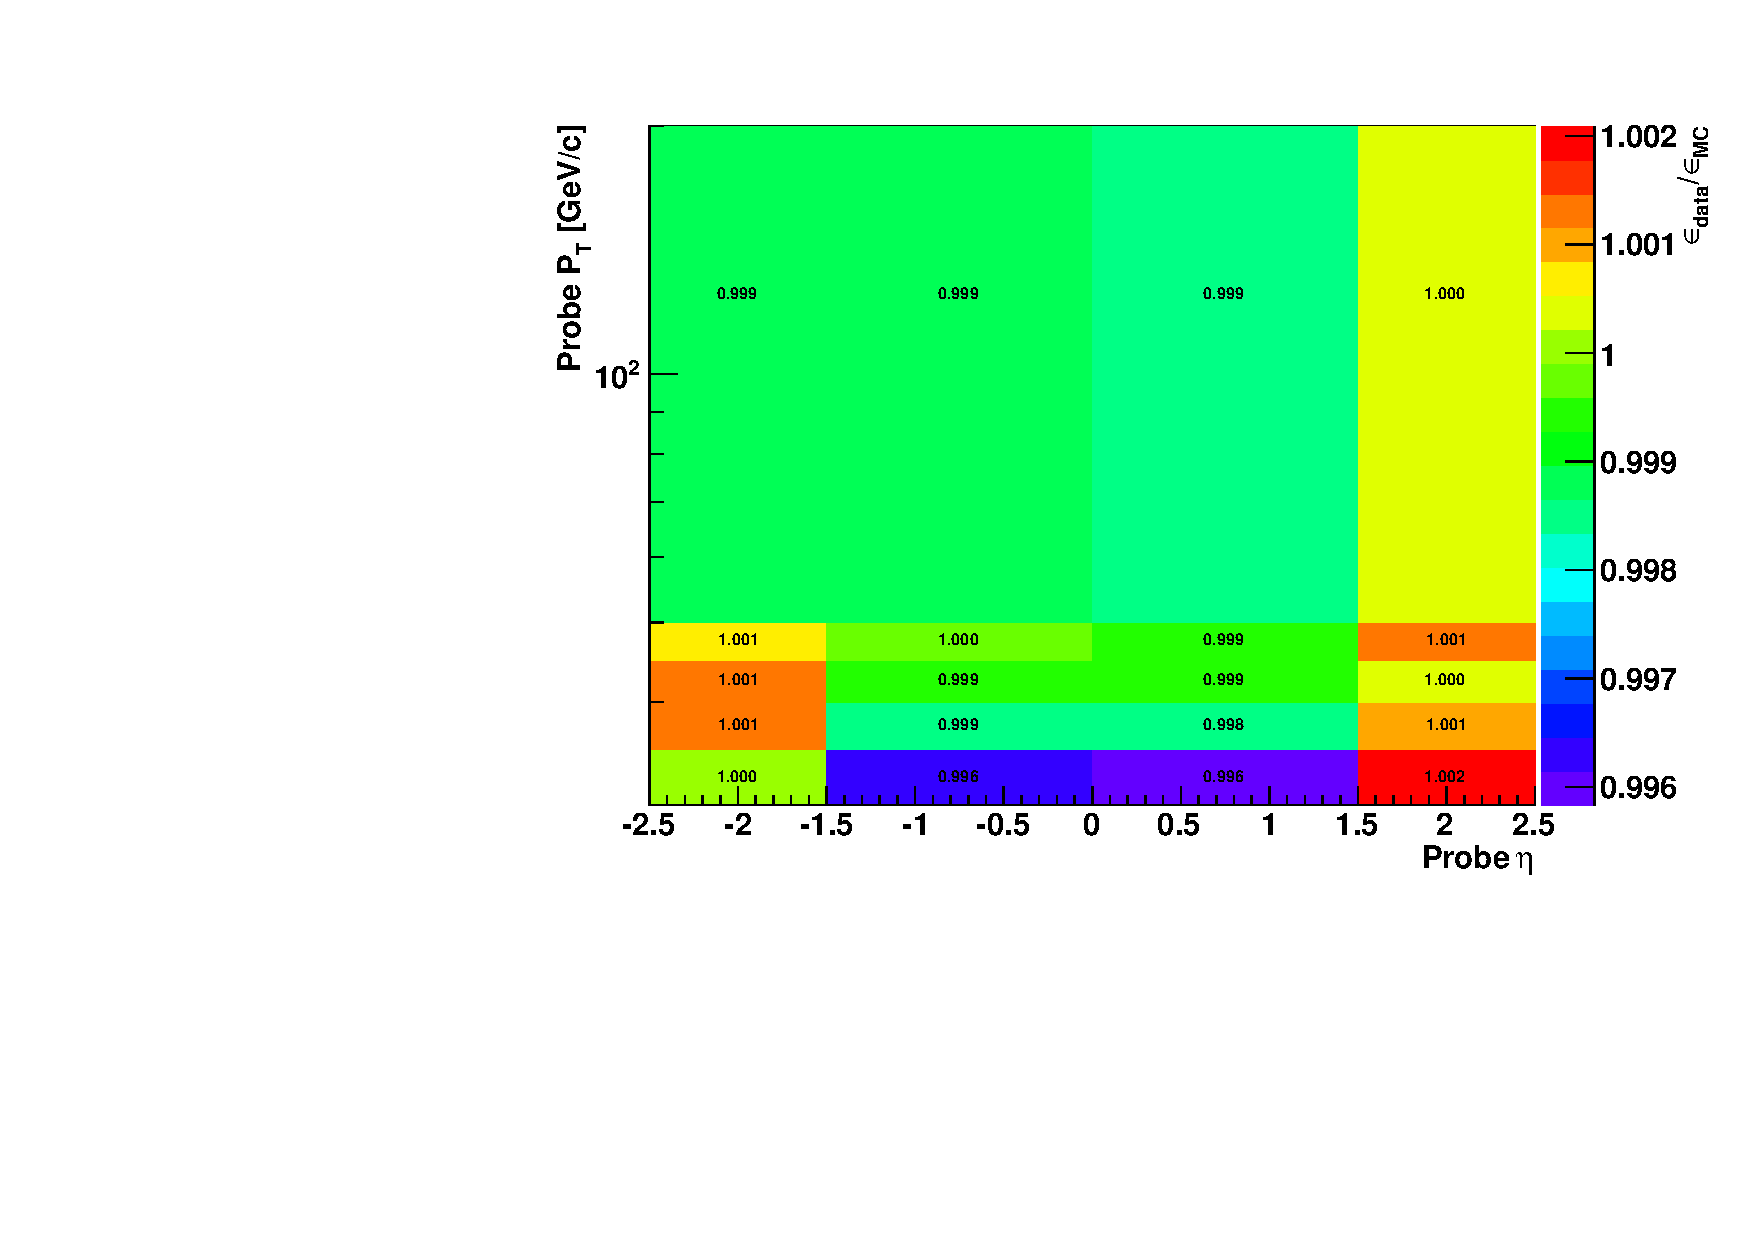
\includegraphics[width=0.32\textwidth]{figs/scaleFactor-Run2012ABC-SCToElectron.pdf}
  }
    \subfigure[]{
    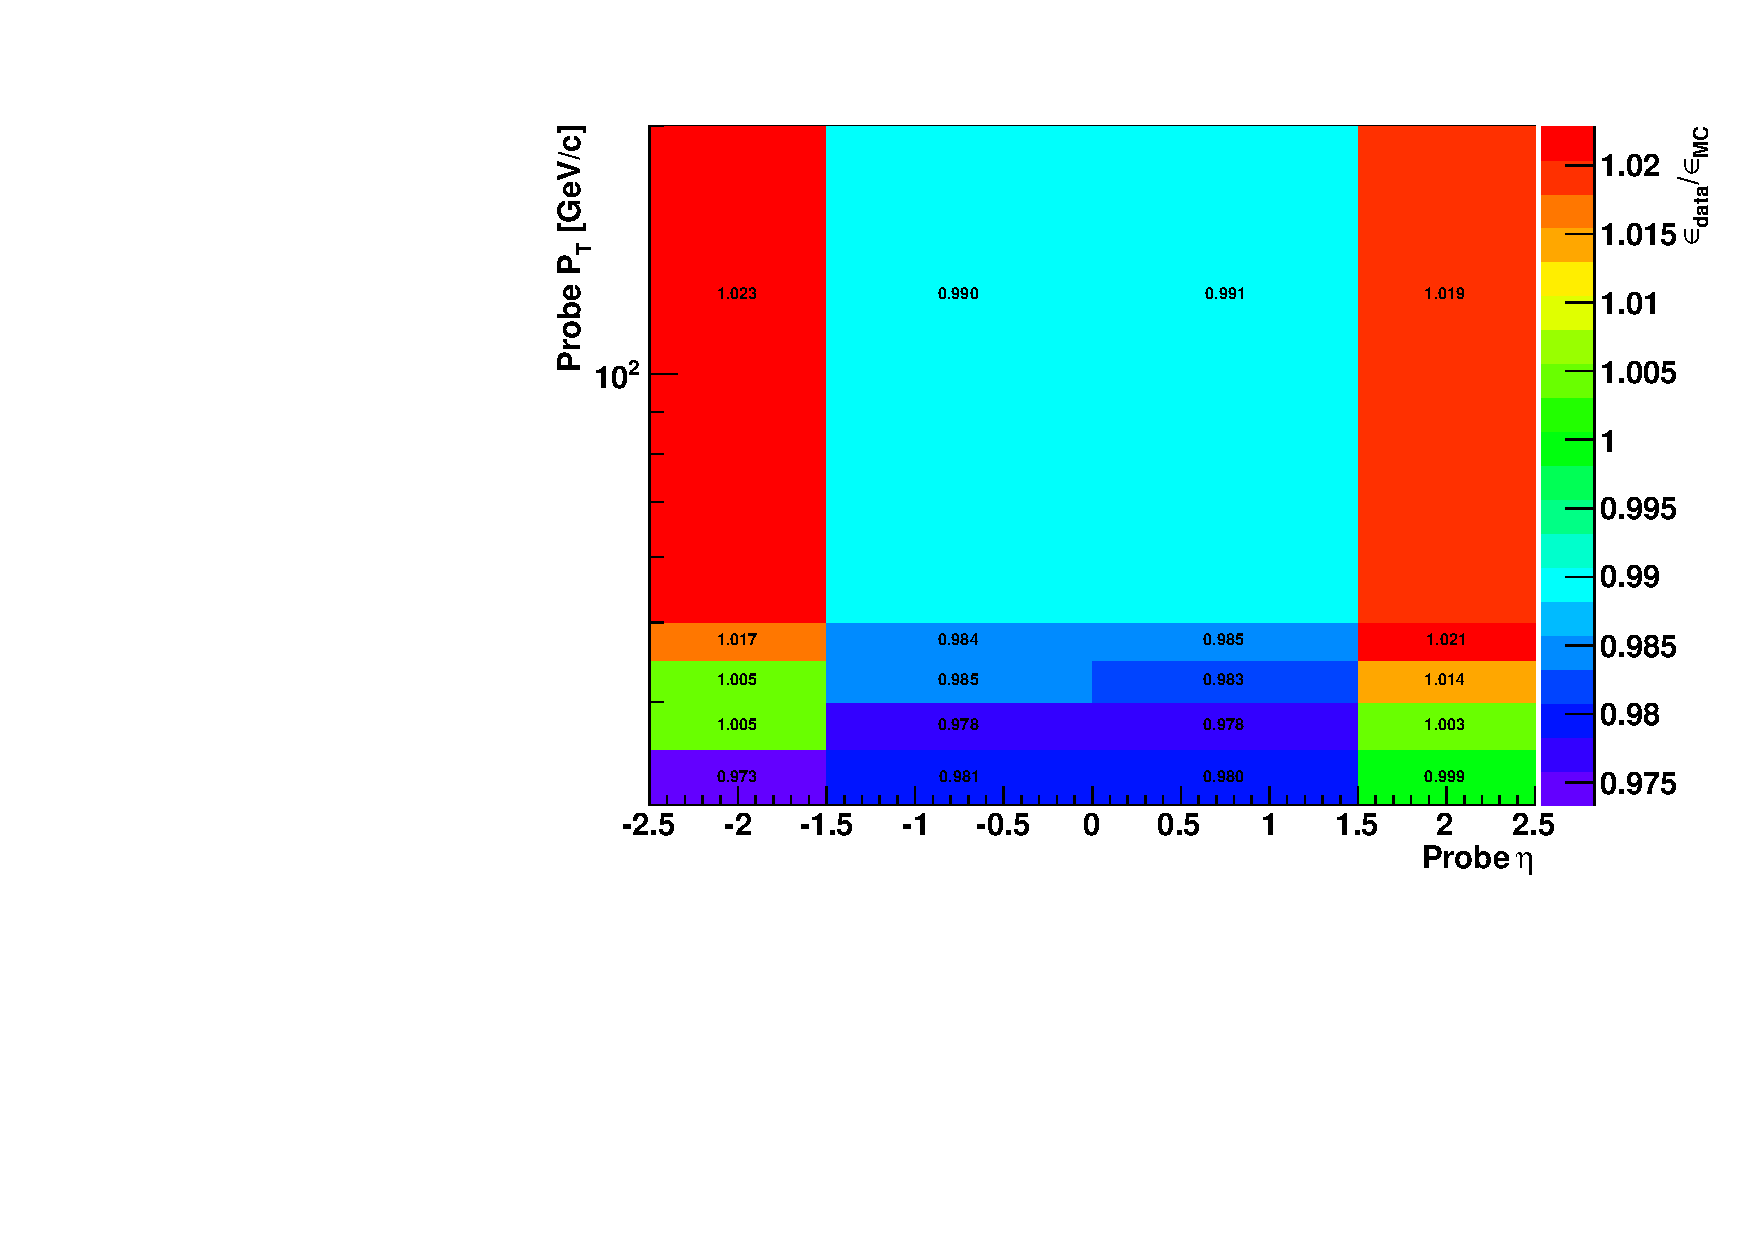
\includegraphics[width=0.32\textwidth]{figs/scaleFactor-Run2012ABC-GsfElectronToId.pdf}
  }
  \subfigure[]{
    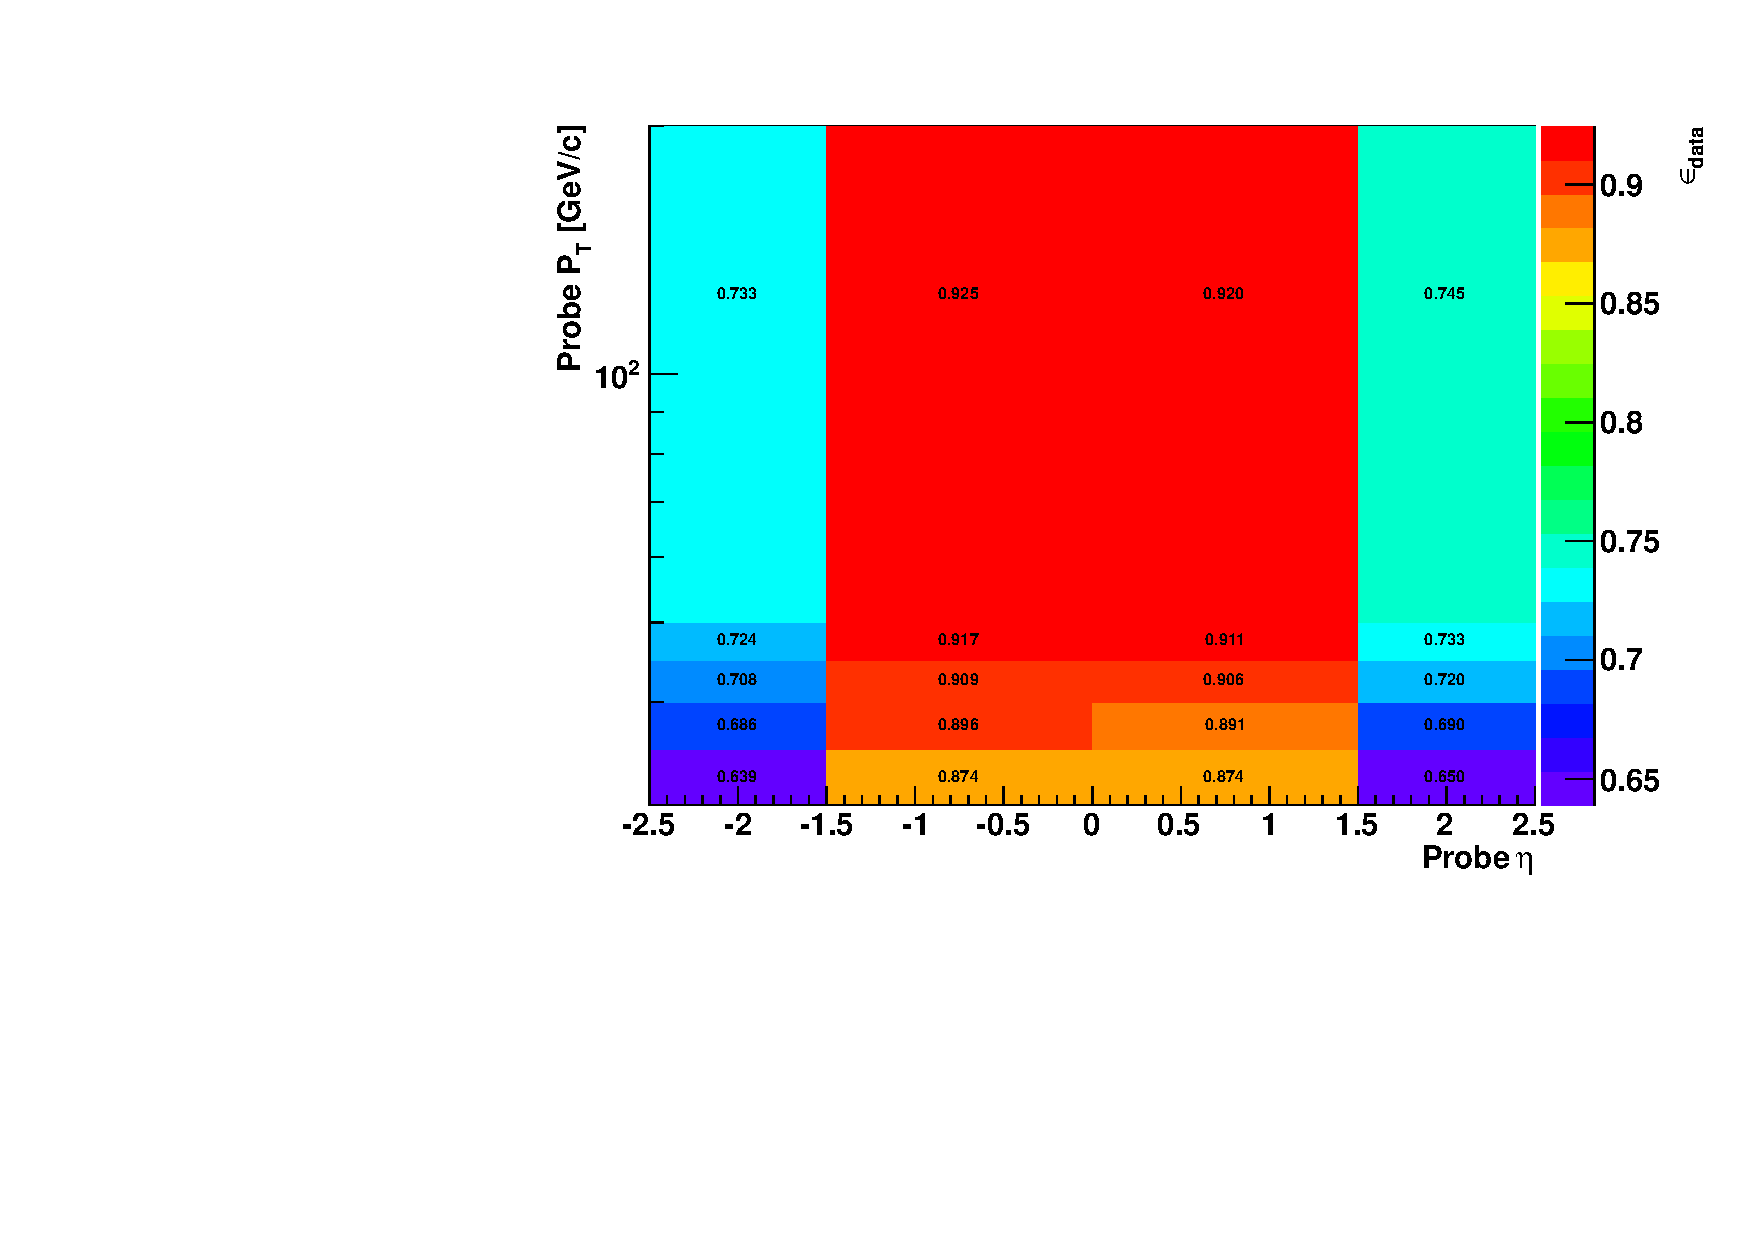
\includegraphics[width=0.32\textwidth]{figs/efficiency-Run2012ABC-WP80ToHLTEle.pdf}
  }
    \caption{Electron efficiency and data/MC scale factors for super-cluster to reconstructed electrons $\epsilon_{\textnormal{Reco}}$ (a),
    reconstructed to selected electrons $\epsilon_{\textnormal{Id}}$ (b) and selected to HLT electrons
      $\epsilon_{\textnormal{HLT}}$ (c).}
    \label{fig:eleEff}
  \end{center}
\end{figure}

\subsection{Muon efficiencies}\label{subsec:EffMu}

In the muon case, the reconstruction efficiency $\epsilon_{\textnormal{Reco}}$ describes the ability to reconstruct a Particle Flow muon starting with
a particle track and can be assumed to be one \cite{MUONPAS}. The identification efficiency $\epsilon_{\textnormal{Id}}$ gives an estimate for a
reconstructed muon to pass the offline selection criteria. It can be computed for both data and simulation and thus a scale factor,
the ratio of the two efficiencies, is derived. \\
The trigger efficiency $\epsilon_{\textnormal{HLT}}$  is the fraction of selected muons fulfilling the HLT requirements, and, since the HLT
requirement is dropped on the MC analysis, the efficiency computed on data is used directly to correct the MC event expectation.\\
The efficiency measurement is binned both in $\pt$ and $\eta$ of the probe muon covering the
relevant intervals (25, 30, 35, 40, 45, 50, 200)\GeVc in $\pt$ and (-2.1, -1.5, -1.0, -0.5, 0.0, 0.5, 1.0, 1.5, 2.1) in $\eta$. The resulting selection
and trigger efficiencies and scale factors are summarized in Table~\ref{tab:muonEff} and Figure~\ref{fig:muonEff}.

\begin{table}[htb]
\centering
\scalebox{0.70}{
  \begin{tabular}{|c|c|c|c|c|c|}
  \hline
  $p_{\textnormal{T,min}}$ & $p_{\textnormal{T,max}}$ & $\eta_{\textnormal{min}}$ & $\eta_{\textnormal{max}}$ & $\epsilon_{\textnormal{ID,data}}$/$\epsilon_{\textnormal{ID,mc}}$ & $\epsilon_{\textnormal{HLT,data}}$ \\
  $[\GeVc]$         & $[\GeVc]$         &                     &                     &                             &                               \\
  \hline
  \hline
  25 & 30 & -2.1 & -1.5 & 0.992 $\pm$ 0.003 & 0.766 $\pm$ 0.003 \\
  25 & 30 & -1.5 & -1 & 0.987 $\pm$ 0.003 & 0.822 $\pm$ 0.003 \\
  25 & 30 & -1 & -0.5 & 0.990 $\pm$ 0.003 & 0.914 $\pm$ 0.002 \\
  25 & 30 & -0.5 & 0 & 0.984 $\pm$ 0.003 & 0.920 $\pm$ 0.002 \\
  25 & 30 & 0 & 0.5 & 0.985 $\pm$ 0.003 & 0.924 $\pm$ 0.002 \\
  25 & 30 & 0.5 & 1 & 0.992 $\pm$ 0.003 & 0.913 $\pm$ 0.002 \\
  25 & 30 & 1 & 1.5 & 0.991 $\pm$ 0.003 & 0.802 $\pm$ 0.003 \\
  25 & 30 & 1.5 & 2.1 & 0.995 $\pm$ 0.002 & 0.814 $\pm$ 0.003 \\
  30 & 35 & -2.1 & -1.5 & 0.991 $\pm$ 0.002 & 0.785 $\pm$ 0.002 \\
  30 & 35 & -1.5 & -1 & 0.988 $\pm$ 0.002 & 0.829 $\pm$ 0.002 \\
  30 & 35 & -1 & -0.5 & 0.988 $\pm$ 0.002 & 0.921 $\pm$ 0.002 \\
  30 & 35 & -0.5 & 0 & 0.984 $\pm$ 0.002 & 0.930 $\pm$ 0.001 \\
  30 & 35 & 0 & 0.5 & 0.985 $\pm$ 0.002 & 0.935 $\pm$ 0.001 \\
  30 & 35 & 0.5 & 1 & 0.990 $\pm$ 0.002 & 0.922 $\pm$ 0.002 \\
  30 & 35 & 1 & 1.5 & 0.987 $\pm$ 0.002 & 0.807 $\pm$ 0.002 \\
  30 & 35 & 1.5 & 2.1 & 0.995 $\pm$ 0.002 & 0.833 $\pm$ 0.002 \\
  35 & 40 & -2.1 & -1.5 & 0.992 $\pm$ 0.002 & 0.793 $\pm$ 0.002 \\
  35 & 40 & -1.5 & -1 & 0.987 $\pm$ 0.002 & 0.832 $\pm$ 0.002 \\
  35 & 40 & -1 & -0.5 & 0.991 $\pm$ 0.002 & 0.926 $\pm$ 0.001 \\
  35 & 40 & -0.5 & 0 & 0.986 $\pm$ 0.002 & 0.935 $\pm$ 0.001 \\
  35 & 40 & 0 & 0.5 & 0.986 $\pm$ 0.002 & 0.940 $\pm$ 0.001 \\
  35 & 40 & 0.5 & 1 & 0.991 $\pm$ 0.002 & 0.925 $\pm$ 0.001 \\
  35 & 40 & 1 & 1.5 & 0.989 $\pm$ 0.002 & 0.812 $\pm$ 0.002 \\
  35 & 40 & 1.5 & 2.1 & 0.994 $\pm$ 0.002 & 0.837 $\pm$ 0.002 \\
  40 & 45 & -2.1 & -1.5 & 0.994 $\pm$ 0.002 & 0.800 $\pm$ 0.002 \\
  40 & 45 & -1.5 & -1 & 0.987 $\pm$ 0.001 & 0.837 $\pm$ 0.002 \\
  40 & 45 & -1 & -0.5 & 0.992 $\pm$ 0.001 & 0.927 $\pm$ 0.001 \\
  40 & 45 & -0.5 & 0 & 0.986 $\pm$ 0.001 & 0.940 $\pm$ 0.001 \\
  40 & 45 & 0 & 0.5 & 0.987 $\pm$ 0.001 & 0.944 $\pm$ 0.001 \\
  40 & 45 & 0.5 & 1 & 0.991 $\pm$ 0.001 & 0.928 $\pm$ 0.001 \\
  40 & 45 & 1 & 1.5 & 0.991 $\pm$ 0.001 & 0.817 $\pm$ 0.002 \\
  40 & 45 & 1.5 & 2.1 & 0.996 $\pm$ 0.001 & 0.844 $\pm$ 0.002 \\
  45 & 50 & -2.1 & -1.5 & 0.993 $\pm$ 0.002 & 0.807 $\pm$ 0.002 \\
  45 & 50 & -1.5 & -1 & 0.987 $\pm$ 0.002 & 0.840 $\pm$ 0.002 \\
  45 & 50 & -1 & -0.5 & 0.990 $\pm$ 0.001 & 0.931 $\pm$ 0.001 \\
  45 & 50 & -0.5 & 0 & 0.988 $\pm$ 0.002 & 0.941 $\pm$ 0.001 \\
  45 & 50 & 0 & 0.5 & 0.987 $\pm$ 0.002 & 0.947 $\pm$ 0.001 \\
  45 & 50 & 0.5 & 1 & 0.992 $\pm$ 0.001 & 0.930 $\pm$ 0.001 \\
  45 & 50 & 1 & 1.5 & 0.991 $\pm$ 0.002 & 0.821 $\pm$ 0.002 \\
  45 & 50 & 1.5 & 2.1 & 0.995 $\pm$ 0.002 & 0.851 $\pm$ 0.002 \\
  50 & 200 & -2.1 & -1.5 & 0.991 $\pm$ 0.002 & 0.809 $\pm$ 0.002 \\
  50 & 200 & -1.5 & -1 & 0.987 $\pm$ 0.002 & 0.842 $\pm$ 0.002 \\
  50 & 200 & -1 & -0.5 & 0.992 $\pm$ 0.002 & 0.931 $\pm$ 0.001 \\
  50 & 200 & -0.5 & 0 & 0.987 $\pm$ 0.002 & 0.944 $\pm$ 0.001 \\
  50 & 200 & 0 & 0.5 & 0.989 $\pm$ 0.002 & 0.946 $\pm$ 0.001 \\
  50 & 200 & 0.5 & 1 & 0.992 $\pm$ 0.002 & 0.932 $\pm$ 0.001 \\
  50 & 200 & 1 & 1.5 & 0.993 $\pm$ 0.002 & 0.824 $\pm$ 0.002 \\
  50 & 200 & 1.5 & 2.1 & 0.996 $\pm$ 0.002 & 0.854 $\pm$ 0.002 \\
  \hline
  \end{tabular}}
\caption{Muon selection scale factors and HLT efficiencies. The errors are statistical only.}
\label{tab:muonEff}
\end{table}


\begin{figure}[t]
  \begin{center}
    \subfigure[]{
    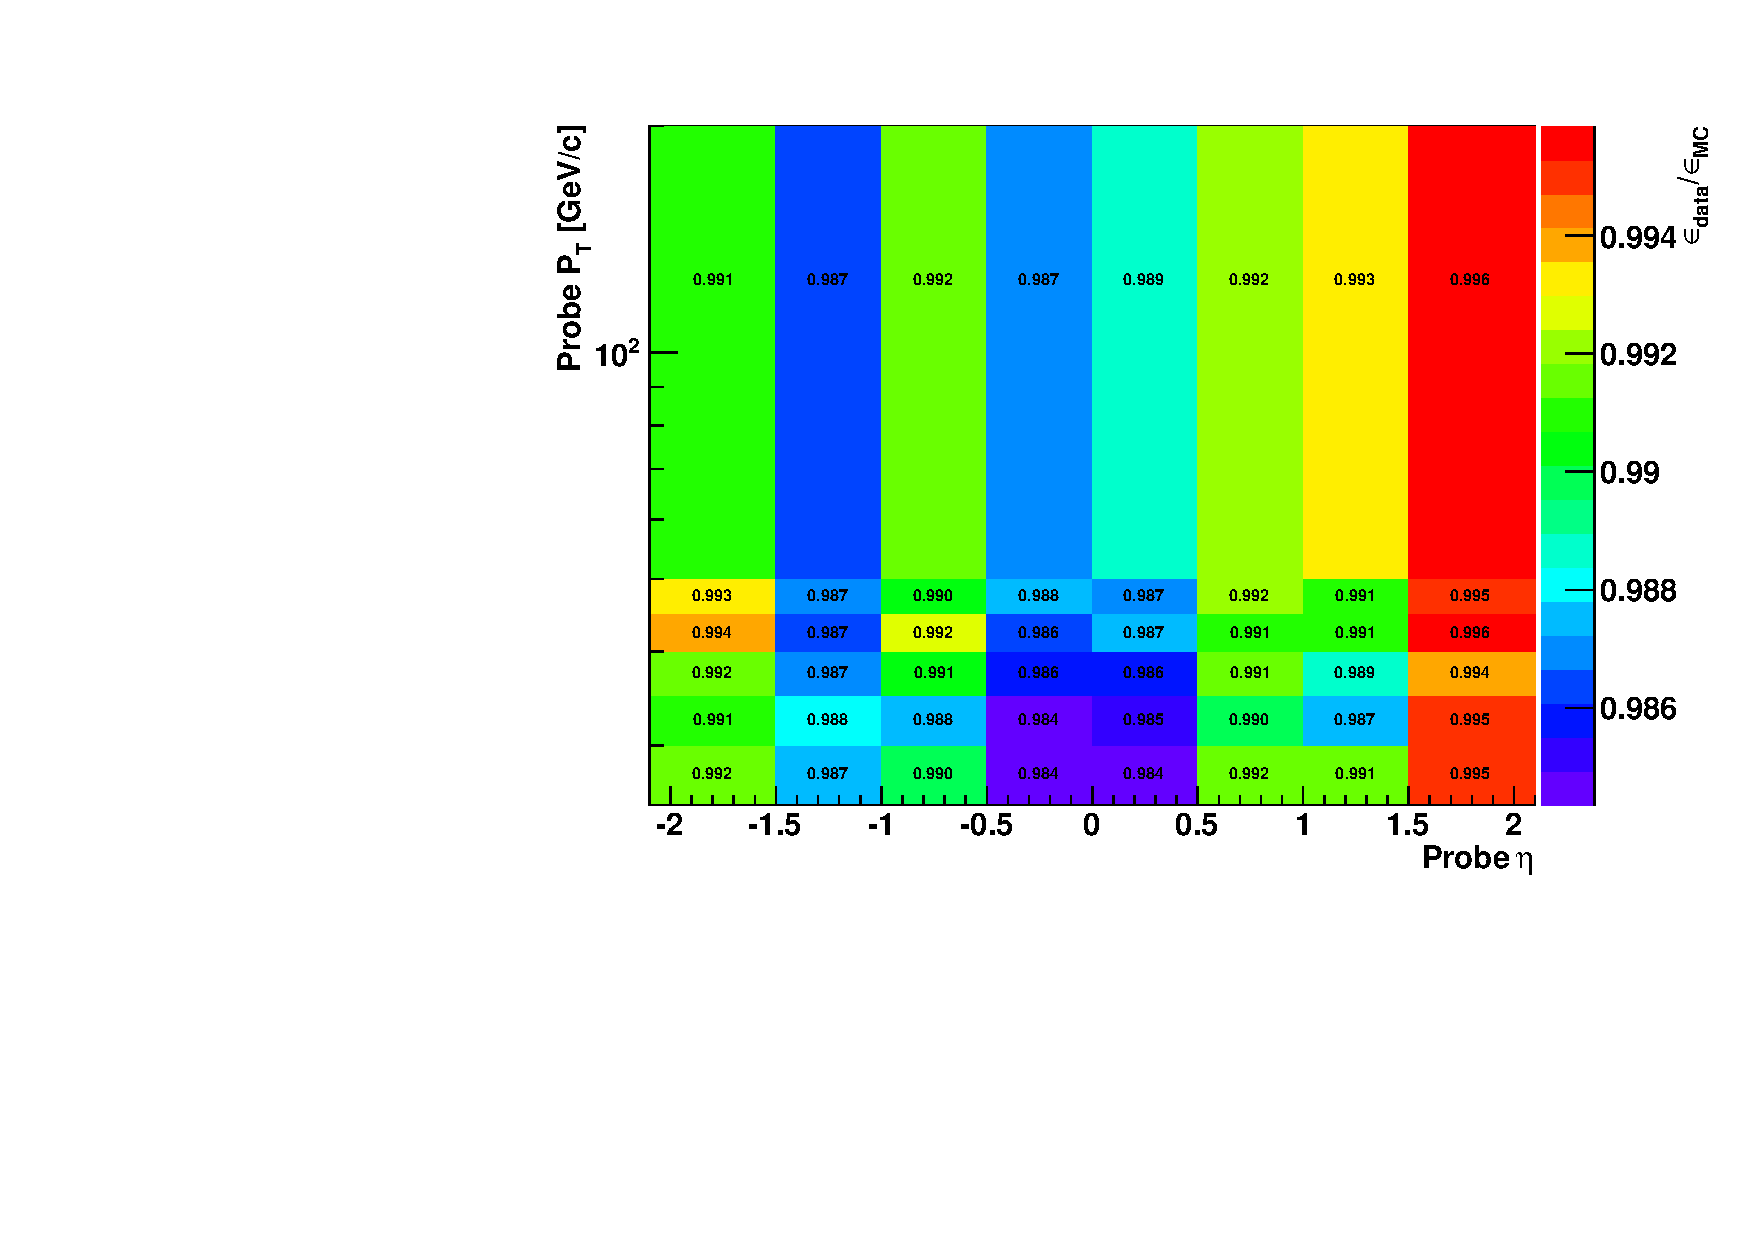
\includegraphics[width=0.47\textwidth]{figs/scaleFactor-Run2012ABC-RecoToIso.pdf}
  }
  \subfigure[]{
    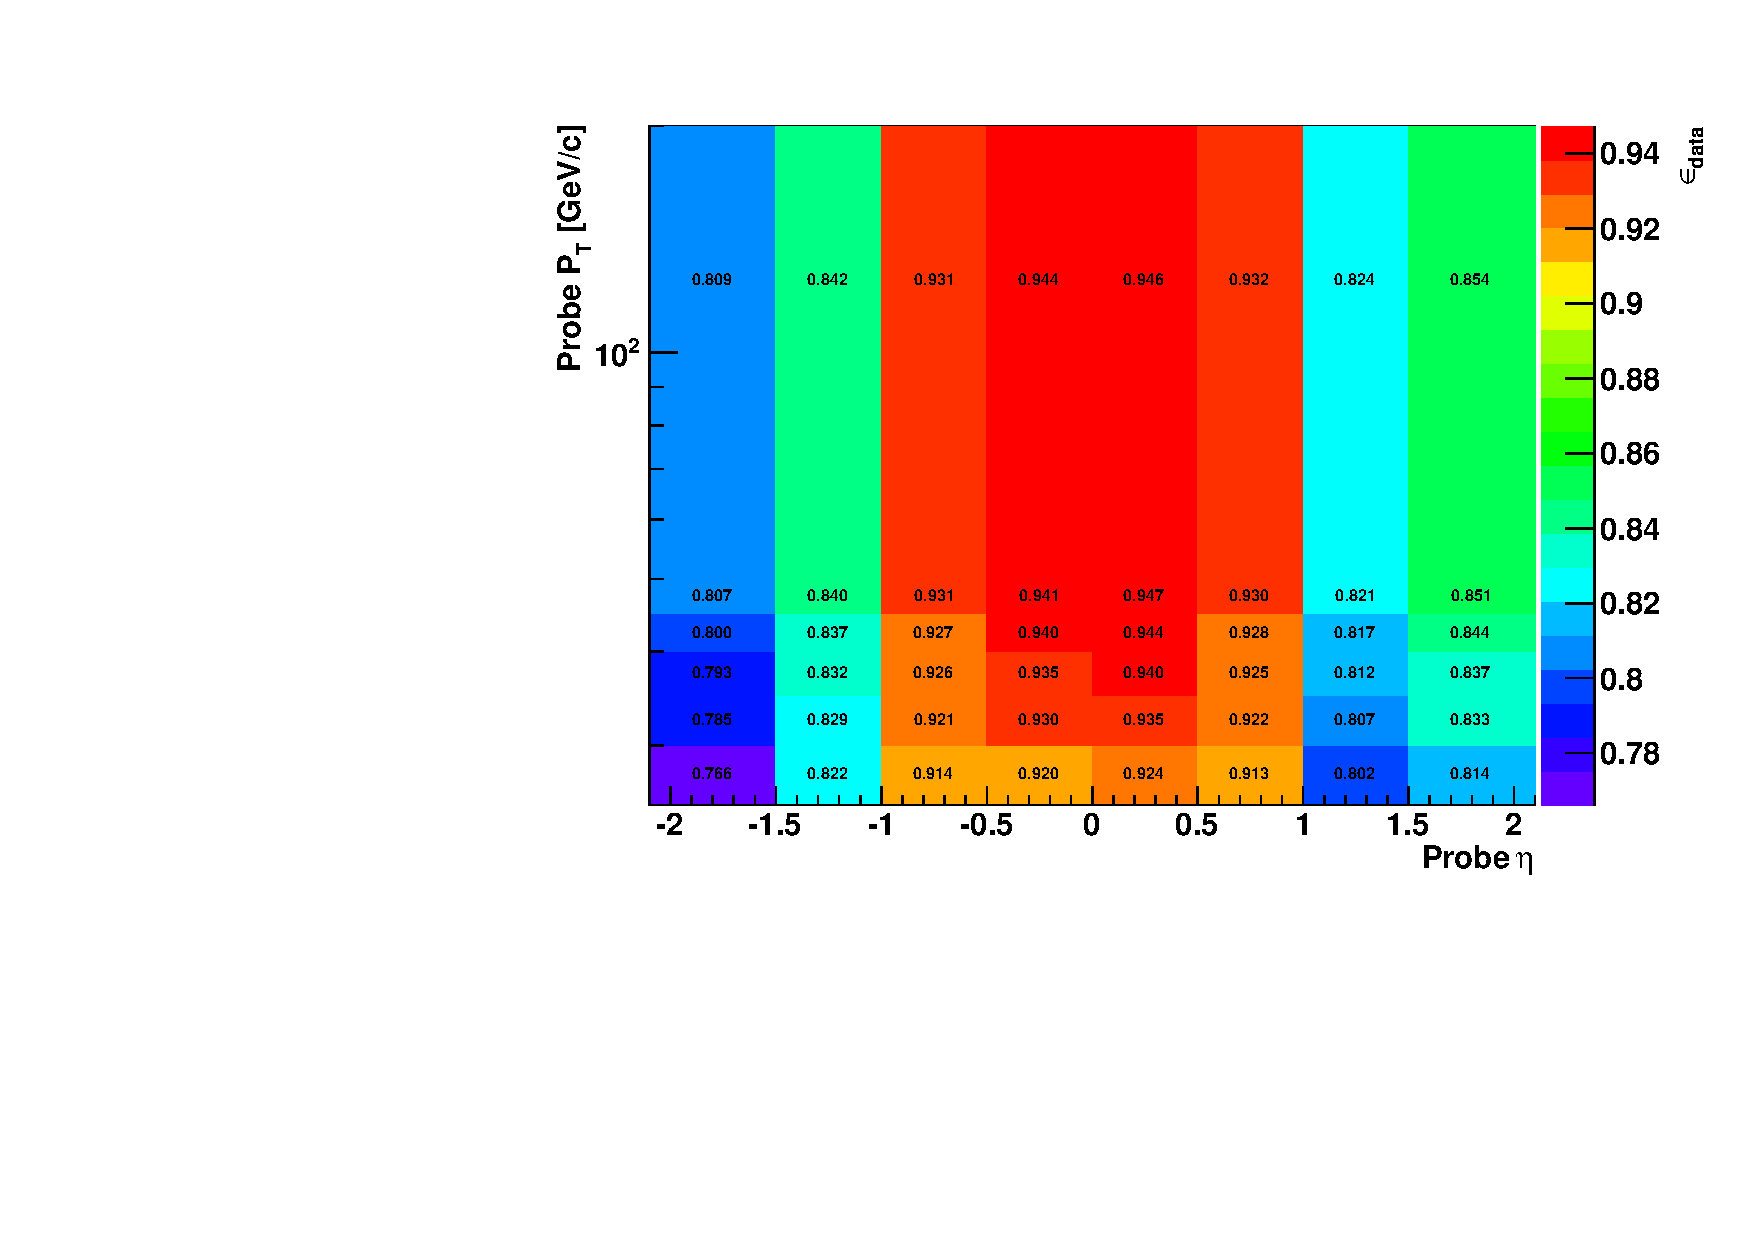
\includegraphics[width=0.47\textwidth]{figs/efficiency-Run2012ABC-IsoToIsoMuHLT.pdf}
  }
    \caption{Muon scale factors for reconstructed to selected muons $\epsilon_{\textnormal{ID,data}}$/$\epsilon_{\textnormal{ID,mc}}$ (a) and
    efficiency for selected to HLT muons $\epsilon_{\textnormal{HLT,data}}$ (b).}
    \label{fig:muonEff}
  \end{center}
\end{figure}



%%%%%%%%%%%%%%%%%%%%%%%%%%%%%%%%%%%%%%%%%%%%%%%%%%%%%%%%%%%%%%%%%%%%%%%%%%
%%%%%%%%%%%%%%%%%%%%%%%%%%%%%%%%%%%%%%%%%%%%%%%%%%%%%%%%%%%%%%%%%%%%%%%%%%
\clearpage{}
\section{Photon reconstruction and fake rate}
\label{sec:photon}
% ---- ---- ---- ---- ---- ---- ---- ---- ---- ---- ---- ---- ---- ---- ----
Photon candidates are reconstructed as SuperClusters in the ECAL with 
$E_{T} > 30 GeV $in the feducial Barrel region, defined by $|\eta|<1.4442$. 
They are required to satisfy 2012 tight cut-based selection 
\cite{pho2012IDcut}, which provides $70\%$ signal selection efficiency:

\begin{itemize}
\item Single tower H/E $<$ 0.05 
\item $0.001 < \sigma_{i\eta i\eta}<0.011$ 
\item PF charged hadron isolation $<$ 0.7, whith charged hadrons originated from the hard interaction primary vertex.
\item pile-up corrected PF neutral hadron isolation $< 0.4 + 0.04*P_{T}^{\gamma}$ 
\item pile-up corrected PF photon isolation $<0.5 + 0.005*P_{T}^{\gamma}$
\item Conversion safe electron veto

\end{itemize}

Isolation is performed for a cone of radius 0.3. Pile-up corrected PF isolation 
is calculated using effective area corrections. The photon candidates are
also required to be separated from the lepton by at least $0.5$ in 
$\eta-\phi$ space, which highly reduces the contribution from FSR to the 
observed photon rate. The same separation requirements are imposed between 
the photon candidates and the jets.

\subsection{Data/MC Efficiency Scale Factors}

We used photon efficiency scale factors for 2012(A+B+C+D) and tight 
photon selection described ~\cite{HtoZA-AN-13-038}, which is Egamma POG 
approved. The scale factors do not include electron veto selection and 
are listed in Table~\ref{tab:photon_eff}. The scale factors for electron 
veto selection are $0.9958 \pm 0.0043 (E_{T}=[30,40] GeV)$ and 
$0.9999 \pm 0.0067 (E_{T}>40 GeV).$ 

\begin{table}[htb]
\centering
    \begin{tabular}{|l|l|c|}
      \hline
      SC $\eta$                     & $E_{T}$ (GeV) & Scale factor  \\ \hline
      \multirow{4}{*}{0.0 - 0.8}    & 30-40         & $0.9711 \pm 0.0020$     \\
                                    & 40-50         & $0.9778 \pm 0.0024$     \\
                                    & 50-Inf        & $0.9718 \pm 0.0014$     \\ \hline
      \multirow{4}{*}{0.8 - 1.4442} & 30-40         & $0.9823 \pm 0.0052$     \\
                                    & 40-50         & $0.9805 \pm 0.0024$     \\
                                    & 50-Inf        & $0.9768 \pm 0.0016$     \\ \hline
    \end{tabular}
  \caption{2012 tight photon ID data/MC efficiency scale factors for given photon $p_{T}$ and $\eta$ ~\cite{HtoZA-AN-13-038}.  }
  \label{tab:photon_eff}
\end{table}

\subsection{2012 Photon ID Fake Rate}

The largest background arises from the $W\gamma$+jets process, while the 
second important contribution comes from jets or electrons misidentified as
a photon. Electrons could be identified as photons due to small track 
reconstruction inefficiency of the detector. This contribution is relevant 
to the electron channel, when an electron or positron from 
$Z\rightarrow ee$ passes the photon identification criteria; therefore, to 
reduce this background, we impose a 
$|M_{Z}-M_{e\gamma}| > \textnormal{10 GeV}$ cut. Events with jets 
misidentified as photons can not be tagged with a simple kinematic 
requirement, because it resembles the topology of the events with true
photons. The adopted approach is to build the expected rate based on the 
ratio method \cite{VgammaPAS}. The method uses a category of 
jets(photon-like jets), which resembles the electromagnetic objects in the 
ECAL, but fail either the isolation or $\sigma_{i\eta i\eta}$ requirement. 
Through simple algebraic conversion it can be made into the photon fake 
rate, or number of fake photon candidates divided by the total number of all
photon candidates. We perform a very similar fake rate estimation using our
full 2012 single lepton dataset and assign a $p_{T}$-dependent systematic
uncertainty on the fake rate estimation. 

Similar to the Egamma method, for our fake rate estimation we use the 
full 2012 dataset with single lepton triggers (that we use in our 
analysis) to form a signal and background template that will be 
normalized to each other's sideband. This is to say that we estimate our 
data-driven fake rate by: filling the signal distribution in 
$\sigma_{I\eta I\eta}$ with 2012 tight photons; filling the background 
distribution in $\sigma_{I\eta I\eta}$ with 2012 photon candidates that fail 
the tight cut in particle flow charged and/or neutral isolation, as well 
as possibly failing the tight $\sigma_{I\eta I\eta}$ cut; and normalizing the
background distribution's $\sigma_{I\eta I\eta}$ sideband (
$\sigma_{I\eta I\eta} >$ 0.011) to the sideband of the signal's distribution.
In order to preserve the sidebands of the signal and background 
$\sigma_{I\eta I\eta}$ distributions, we remove the $\sigma_{I\eta I\eta}$ cut in
the 2012 tight photon ID. We normalize the background's sideband to the 
signal sideband because we call any photon candidates that fail the tight
$\sigma_{I\eta I\eta}$ a fake photon, or photon-like jet; therefore, any
contribution in the signal distribution above $\sigma_{I\eta I\eta} >$ 0.011
comes from the background, or fake photons. 
Figure~\ref{fig:normalizeFake} demonstrates how the backgrounds' 
sidebands have been normalized to the signals' sidebands for each photon
$p_{T}$ bin.

\begin{figure}[]
  \begin{center}
    \subfigure[]{
    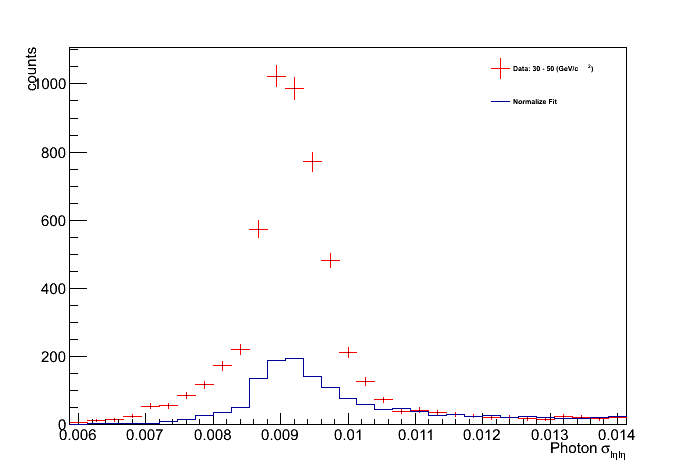
\includegraphics[width=0.33\textwidth]{figs/normalize_fit_30_to_50.png}
  }
    \subfigure[]{
    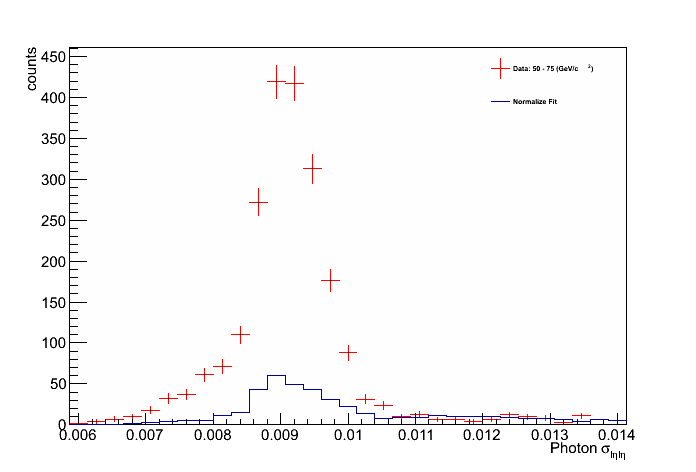
\includegraphics[width=0.33\textwidth]{figs/normalize_fit_50_to_75.png}
  }
    \subfigure[]{
    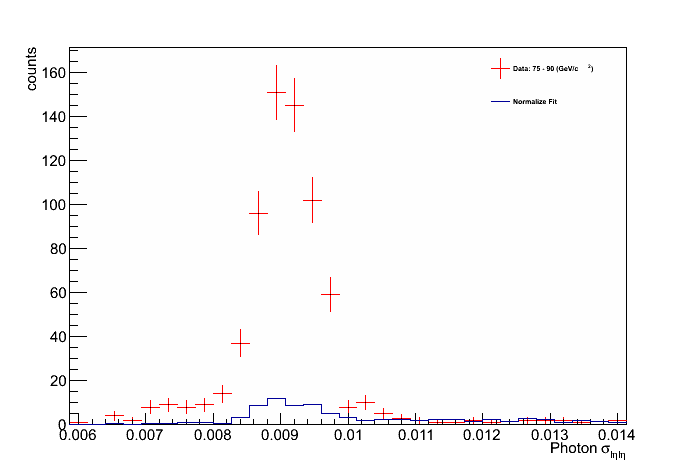
\includegraphics[width=0.33\textwidth]{figs/normalize_fit_75_to_90.png}
  }\\
    \subfigure[]{
    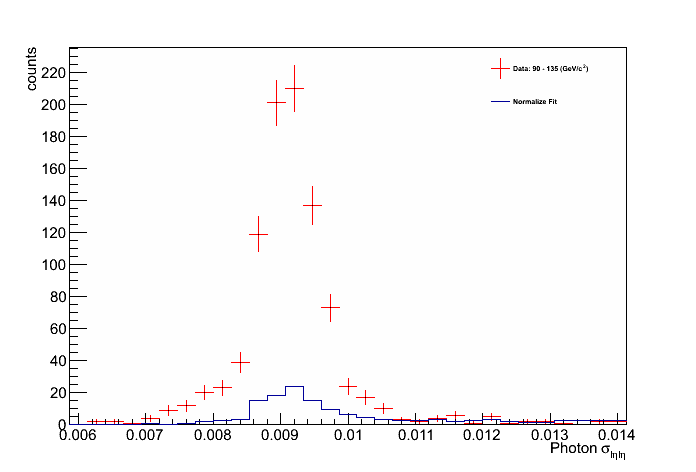
\includegraphics[width=0.33\textwidth]{figs/normalize_fit_90_to_135.png}
  }
    \subfigure[]{
    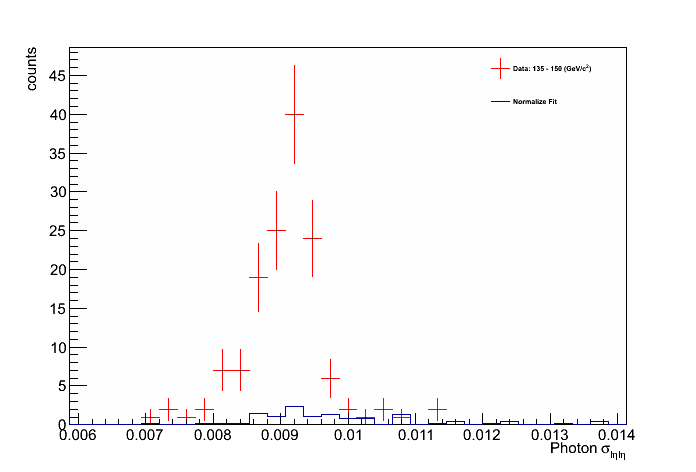
\includegraphics[width=0.33\textwidth]{figs/normalize_fit_135_to_150.png}
  }
    \subfigure[]{
    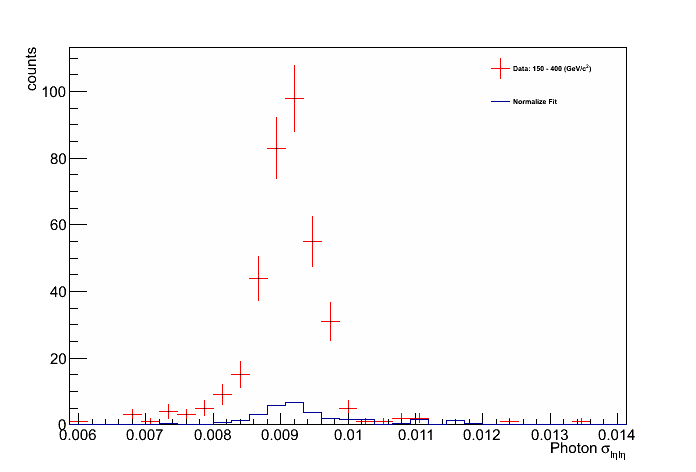
\includegraphics[width=0.33\textwidth]{figs/normalize_fit_150_to_400.png}
  }
    \caption{Signal and background distributions in $\sigma_{I\eta I\eta}$ used to estimate the WW$\gamma$ photon-like jet, or fake photon, rate. Red points are from 2012 tight photons, while blue points are 2012 photon candidates that fail tight PF charged and/or neutral isolation. The background's sideband (above 0.011) is normalized to the signal. Photon $p_{T}$: (a) 30-50 GeV/c, (b) 50-75 GeV/c, (c) 75-90 GeV/c, (d) 90-135 GeV/c, (e) 135-150 GeV/c, (f) 150-400 GeV/c}
    \label{fig:normalizeFake}
  \end{center}
\end{figure}

With the two distributions' sidebands normalized in each photon $p_{T}$ 
bin, we estimate the fake-photon contamination within the signal 
distribution by integrating the background below $\sigma_{I\eta I\eta}$ of 
0.011. Thus, with the number of background, or photon-like jets, and the 
number of 2012 tight photons below this cut, we can estimate our 
analysis's $p_{T}$-dependent photon fake rate, as shown in 
Table~\ref{tab:WWAfakerate}. We only estimate the rate for barrel photons
currently.

\begin{table}[bthp]
\begin{center}
{\footnotesize
\begin{tabular}{|c|c|}
\hline
Photon $p_{T}$, & Fraction of events with jets,\\
GeV & passing tight photon ID\\

\hline
30-50    &  0.229\\
50-75    &  0.156\\
75-90    &  0.091\\
90-135   &  0.122\\
135-150  &  0.080\\
150-400  &  0.077\\
\hline
\end{tabular}
\caption[.]{\label{tab:WWAfakerate}
WV$\gamma$ Fake rate from q-jets and tight 2012 photon ID.}}
\end{center}
\end{table}

In order to estimate the systematic uncertainty in the photon fake rate,
two separate contributions are considered - the effect of biasing the
fake photon template, and the statistical uncertainty in the bias
measurement. The known bias is that the fake photon template is
constructed using inverted PF isolation in the 2012 photon tight selection
ID, where it is assumed that all photon candidates filling this template
are in fact jets faking a photon.  

To test this bias, a MC sample
containing jets misidentified as photons is used (such as W+jets MC), along with its
generator information for all jets and photons, to construct the truth
and estimate templates. The muon channel of the MC is used for this study
in order to remove the photon-faking electron contribution.  The generator information 
is used to remove all ISR/FSR
photons from the pool of 2012 tight photon candidates in the MC, leaving only
those photon candidates that must be jets misidentified as photons - these will
fill the truth template. The estimate template is filled using the aforementioned
inverted isolation procedure for all photon candidates in the MC. The two
templates are compared using the same prescription described for the data-driven
fake rate estimate of the prompt and fake photon templates; however, due to low
statistics in MC after removing all prompt photons, the entire photon $p_{T}$ range
is used to fill one truth template and one estimate template. Any deviation from a
100\% match between the true and estimate templates is considered to be the
measurement of the bias. The bias is measured to be -6\% $\pm$ 11\%, or that the 
truth and estimate templates are in 94\% agreement. The uncertainty in this measurement
is included in the overall systematic uncertainty in the fake rate.

The photon $p_{T}$-dependent statistical uncertainty is estimated using toy MCs -
histograms filled with similar statistics as those of the data-driven fake photon
templates, using a random filler. The toy MC histograms
are then treated as the new fake photon templates, while still using the data-driven
prompt photon templates, and the fake photon rate is
remeasured. The RMS of the measurement of the fake rate for all toy MCs is made
the statisticly-driven uncertainty in the fake rate systematic uncertainty. Table~\ref{tab:fakerate_unc}
contains the photon $p_{T}$-dependent statistical uncertainties in the fake rate, where
the last two photon $p_{T}$ bins mentioned earlier (135-150 GeV and 150-400 GeV) have
been combined due to low statistics. The measured systematic and statistical uncertainties
are combined to make the photon $p_{T}$-dependent systematic uncertainties listed in 
Table~\ref{tab:sys_unc}.

\begin{table}[htb]
\centering
    \begin{tabular}{|c|c|c|c|c|}
      \hline
      $E_{T}$ (GeV) & Fake Rate & Stat. Unc. & Stat. Unc. (\%) & Bias Stat. Unc. (\%)  \\
      \hline
      30-50         & 0.229     & 0.0128     & 5.6             & 11 \\
      50-75         & 0.156     & 0.0147     & 9.4             & 11 \\
      75-90         & 0.091     & 0.0184     & 20              & 11 \\
      90-135        & 0.122     & 0.0230     & 19              & 11 \\
      135-400       & 0.078     & 0.0287     & 37              & 11 \\
      \hline
    \end{tabular}
  \caption{2012 tight photon ID data-driven photon-faking jet rate plus uncertainties for given photon $p_{T}$.  }
  \label{tab:fakerate_unc}
\end{table}

When selecting fake-photon events from our data in order to complete our
analysis for aQGC, the photon-like jet selection satisfies 2012 loose 
cut-based selection \cite{pho2012IDcut}, while it is also required to 
fulfill at least one of following:

\begin{itemize}
\item $\sigma_{i\eta i\eta}>0.012$
\item PF charged hadron isolation $> 4.0 $
\item pile-up corrected PF neutral hadron isolation $> 4.5 +0.04*P_{T}^{\gamma}$
\item pile-up corrected PF photon isolation $>4.5 + 0.005*P_{T}^{\gamma}$

\end{itemize}

These events are then weighted according to the fake ratio derived from
our fake rate.

%We also restrict our analysis to barrel photons by imposing a $|{\eta}| < \textnormal{1.4442}$ cut.  We choose to ignore events with photons detected in the endcaps because the rate of falsely identified photons, or fake photons, as well as the systematics for estimating such a rate, increases outside of the barrel region.  A $p_{T}$ threshold of 30 GeV is used, also due to the fake photon rate that will be discussed - specifically because the rate is only defined down to photon $p_{T}$ of 32 GeV.  Another fake photon contribution considered is that of a Z boson decaying to two electrons, where one of the electrons gets misidentified as a photon; therefore, to reduce this background we impose a $|M_{Z}-M_{e\gamma}| > \textnormal{10 GeV}$ cut.  All selected photons are also required to be isolated from jets and leptons with an isolation cone of size 0.5 or greater.

%The Vgamma photon fake rate considered jets consisting of $\pi_{0}\textnormal{'s}$.  In order to estimate the rate of such jets being misidentified as photons, they performed a two-component template fit using 2011 A\&B photon secondary datasets and a diphoton Monte Carlo sample.  The data and Monte Carlo signal templates were created using the 2011 tight photon ID mentioned earlier, without the sigmaIetaIeta cut, while the Monte Carlo background template used all the same cuts with the exception of inverting the Track isolation cut.  The sigmaIetaIeta cut was removed from the templates in order to preserve the sidebands used in the template fit.  Since the photon fake rate is also known to be dependent on both $\eta$ and photon $p_{T}$, the templates were made for specific $\eta$ and photon $p_{T}$ ranges and compared in the final result shown in Figure~\ref{fig:fkrate}.

%The distribution shown in Figure~\ref{fig:fkrate} is the photon fake ratio, or the number of fake photon candiates divided by the number of true photon candidates, and through algebraic conversion it can be made into the photon fake rate, or number of fake photon candidates divided by the total number of all photon candidates.  In order to use this Vgamma photon fake rate in our analysis, we fit the distribution shown above with a function and applied it as a weight scale factor on the 2012 full dataset.  This means that the function estimates what fraction of the observed data events are likely to include a jet misidentified as a photon.


%%%%%%%%%%%%%%%%%%%%%%%%%%%%%%%%%%%%%%%%%%%%%%%%%%%%%%%%%%%%%%%%%%%%%%%%%%
%%%%%%%%%%%%%%%%%%%%%%%%%%%%%%%%%%%%%%%%%%%%%%%%%%%%%%%%%%%%%%%%%%%%%%%%%%
\clearpage{}
\section{K-factors}
\label{sec:Kfact}

\subsection{\wwa signal K-factor}

Leading-order samples generated by MadGraph5 are used for this analysis. 
Generally, LO calculations can provide a good estimation of cross sections 
and a description of kinematic distributions, but the shortcoming is also 
obvious. Its dependence on the unphysical renormalization and factorization 
scales can result in a large theoretical uncertainty, especially for those 
processes with large logarithms. Therefore, NLO calculations are important 
for precise analysis. In an experimental analysis, generally one can use a 
K-factor, which is defined as the ratio of the NLO to LO cross section for 
a given process, to estimate the NLO effect. However, its dependence on the 
renormalization and factorization scales, as well as the parton distribution
functions (PDFs), should result in large uncertainties. Moreover, the NLO 
corrections can also lead to shape changes in kinematic distributions, 
especially when tight cuts are applied. Thus, one needs to make a careful 
examination to get a reasonable K-factor.

The emerging package aMC@NLO ~\cite{Frederix:2011zi,Frederix:2011qg} 
implements automatic event generation with NLO accuracy, which is a great 
improvement of MC hard events generation. However, we do not use the NLO 
samples for our analysis. Instead, we investigated the K-factor distribution
as a function of the photon $p_{T}$, which gives us reasonable K-factors for
our \wwa samples. 

For our analysis, 200k \wwa signal events, without W decays, are first 
generated using aMC@NLO. Then the samples are passed to 
HERWIG~\cite{Corcella:2000bw} to do parton shower. In the framework of 
aMC@NLO, theoretical uncertainties can also be obtained through a 
process-independent technique introduced in Ref.~\cite{Frederix:2011ss}, 
which allows aMC@NLO to compute scale and PDF uncertainties in a fully 
automated way and at no extra CPU-time cost. The default renormalization and
factorization scales are set equal to the sum of transverse masses of all 
final state particles and partons. To get scale dependence, we vary the 
$\mu_R$ and $\mu_F$ independently, considering the set of 
$(\mu_R,\mu_F) = (\kappa_R \mu_R,\kappa_F \mu_F)$, with \\ 
%%
$(\kappa_R,\kappa_F) = (1, 1), (1/2, 1/2), (2, 2)$\\
%%
and the overall scale uncertainty is the maximum deviation of all the sets.
The PDF uncertainty is estimated following the method (asymmetric Hessian) 
illustrated in Ref.~\cite{Martin:2009iq}. The 
$MSTW2008nlo68cl$~\cite{Martin:2009iq} PDF sets are used for this analysis 
which contains 20 pairs to compute PDF uncertainties.

To make the result close to the experimental analysis, some basic cuts
have been applied for the samples. $p_{T_{\gamma}} > 10 \text{GeV}$
and $|\eta_{\gamma}| < 2.5$ have been used for both LO and NLO
calculation.  As for photon isolation cut, the cone approach is not
infrared safe for NLO calculation. Therefore, we adopted the isolation
cut introduced in Ref.~\cite{Frixione:1998jh, Bozzi:2009ig}instead: if
$i$ is a parton with transverse energy $E_{T_{i}}$ and a separation
$R_{i_{\gamma}}$ with a photon of transverse momentum $p_{T_{\gamma}}$,
then the event is accepted only if:

\begin{equation}
\sum_i E_{T_i} \theta ( \delta - R_{i{\gamma}} ) \leq p_{T_{\gamma}} \frac{ 1 - cos \delta }{ 1 - cos \delta_0 } \text{    } ( \text{  for all } \delta \leq \delta_0 )
\label{nloacut}
\end{equation} 

where $\delta_0$ is fixed to be 0.7. 

\begin{figure}[]{
\centering
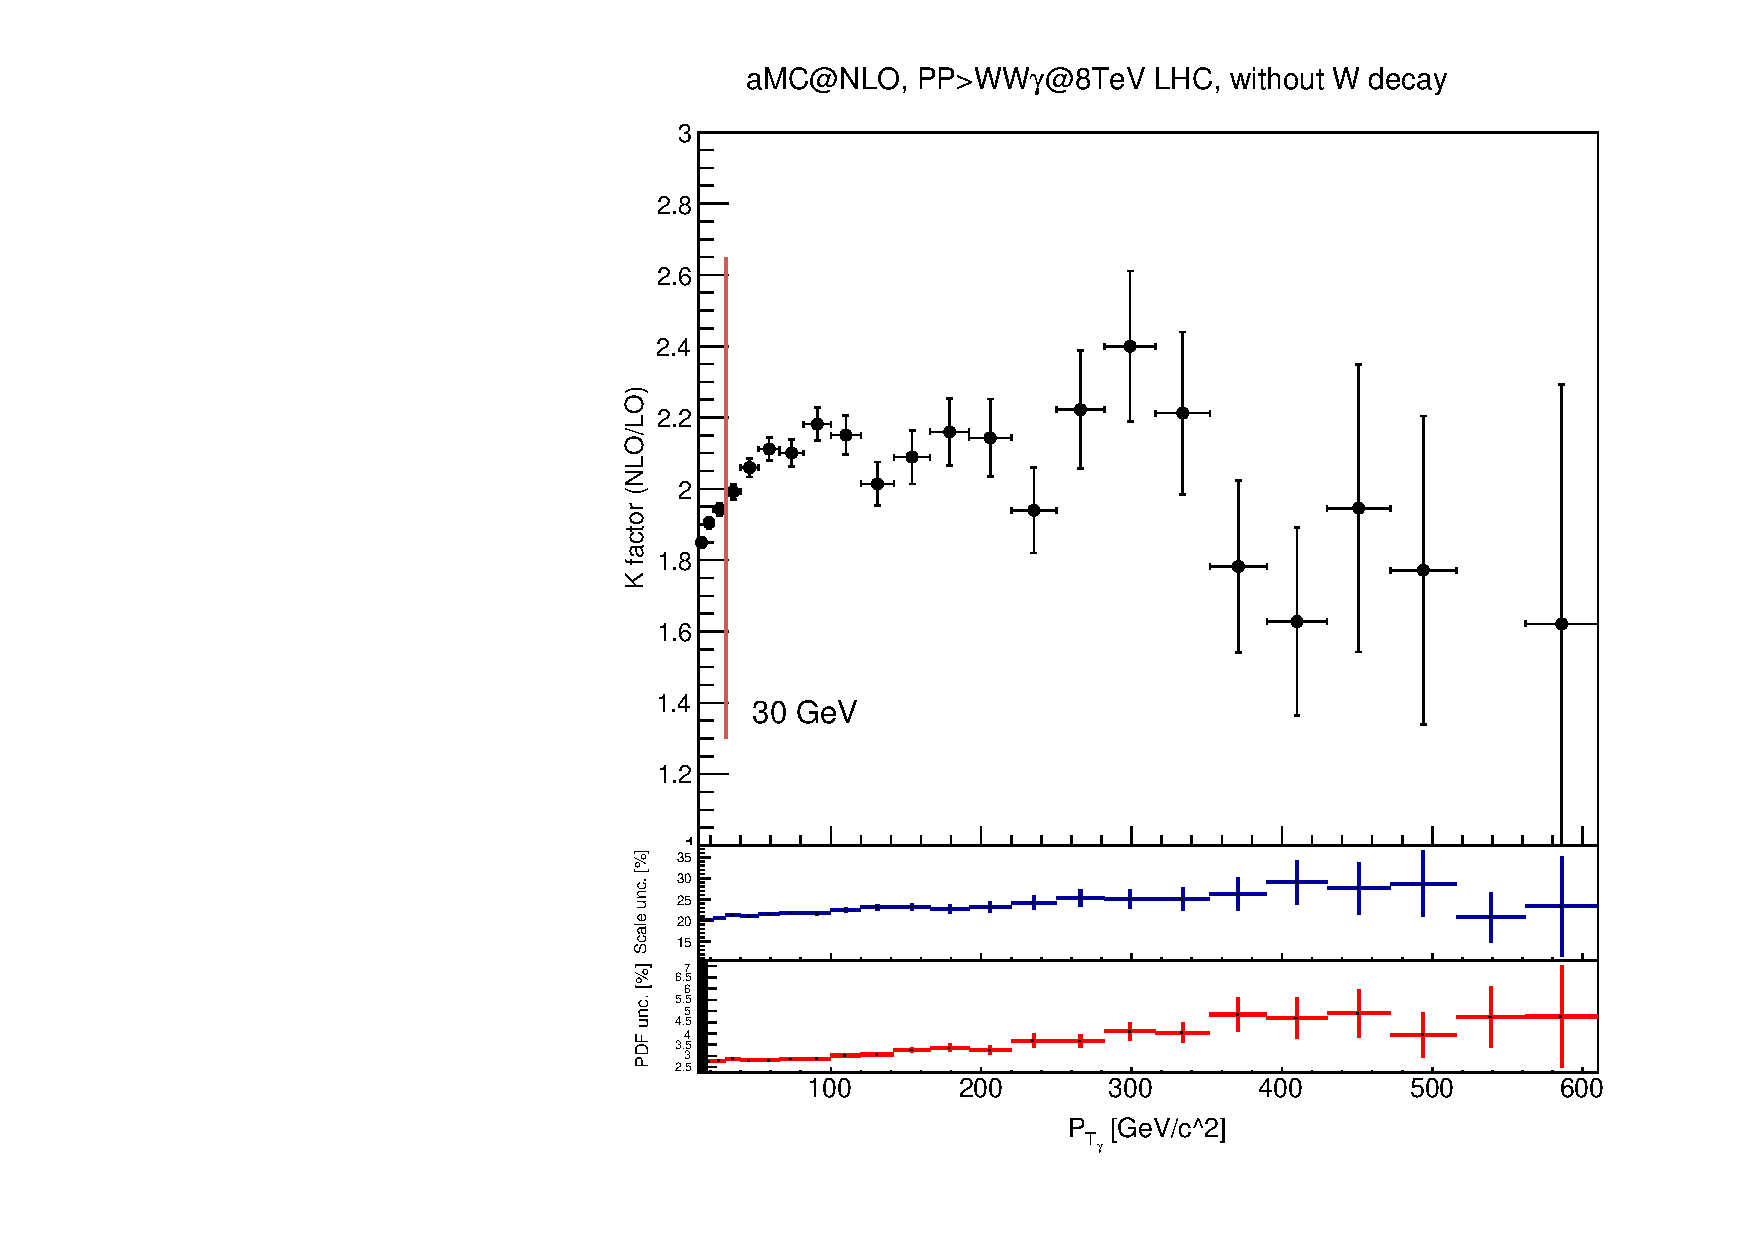
\includegraphics[width=0.4\textwidth]{figs/kwwa_pt.pdf}
\caption{\label{k-wwa} \wwa signal sample K-factor distribution as a function of $p_{T_{\gamma}}$.}}
\end{figure}

In Figure~\ref{k-wwa}, the K-factor distribution is quite flat; we use a Binned Likelihood method fit to a constant to get the value of the K-factor. 
Therefore, the K-factor value, with scale and PDF uncertainties, we use for 
the SM signal sample is 2.09812 $\pm$ 0.302029\% (stat.) $\pm$ 23.4256\% 
(scale) $\pm$ 3.55719\% (PDF).

\newpage
\subsection{aQGC K-factor}
\label{sec:aQGC_Kfac}

The MC samples for aQGC study are generated as SM WV$\gamma$ with added aQGC.
K-factor for two values of $a_{0}^{W}/\Lambda^{2}$ and $a_{C}^{W}/\Lambda^{2}$ are computed 
as function of the photon $p_{T}$ and show on Figure~\ref{k-Awwa}. At low photon $p_{T}$ the 
K-factor resembles the SM WW$\gamma$ K-factor, while with the increase of the photon $p_{T}$, most of 
the contributions are from the quardrilinear diagrams, and one can expect that the value will be similar to the Drell Yan processes.
The K-factor $p p \rightarrow W^{+}$ and $ p p \rightarrow Z$ processes have been also calculated , and the results turned out to be 
1.185 and 1.184. As can be seen in Figure~\ref{k-Awwa}, the aQGC K-factor levels at approximately 1.185 when the
photon $p_{T}$ is greater than 300 GeV/c. The exact behavior of the K-factor at low photon $p_{T}$ for the SM WW$\gamma$ with added aQGC 
depends on type of the aQGC parameter and its value. On Figure~\ref{k-Awwa} is shown the K-factor for two different aQGC parameters, 
while on Figure~\ref{k-diffvalue} is shown the K-factor for two different values of the same aQGC parameters, namely 
$a_{0}^{W}/\Lambda^{2}$.

In this study we define as visible aQGC signal only the contribution, which is originated from the anomalous quardrilinear diagrams.
The limit-setting machinery, discussed
in Section~\ref{sec:aQGClim}, uses a signal input distribution which is the
difference between the SM WV$\gamma$ with added aQGC and SM WV$\gamma$ only photon $p_{T}$ distributions (refer to as "aQGC-SM").
Since virtually all events with a photon $p_{T}$ above 300 GeV/c are predicted to
be from aQGC in our analysis, then the input distribution should reflect the
K-factor of 1.185 only. To accomplish this, when preparing the input file 
for the limit setter, we do not use a K-factor for either the SM or aQGC 
samples in the aQGC-SM subtraction. With the resulting aQGC-SM distribution
being primarily high photon $p_{T}$ events, and aQGC in nature, then we
apply the K-factor of 1.185. Since there are some remaining low photon 
$p_{T}$ aQGC events in the aQGC-SM distribution, we are applying a constant
K-factor across the board. An illustration of the resulting K-factor from such procedure is shown on Figure~\ref{k-pureaqgc}.
Photon $p_{T}$ distributions for aQGC-SM LO and NLO samples are shown on \ref{k-pureaqgc}a, while the resulting K-factor is 
shown on \ref{k-pureaqgc}b. 

\begin{figure}[]{
\centering
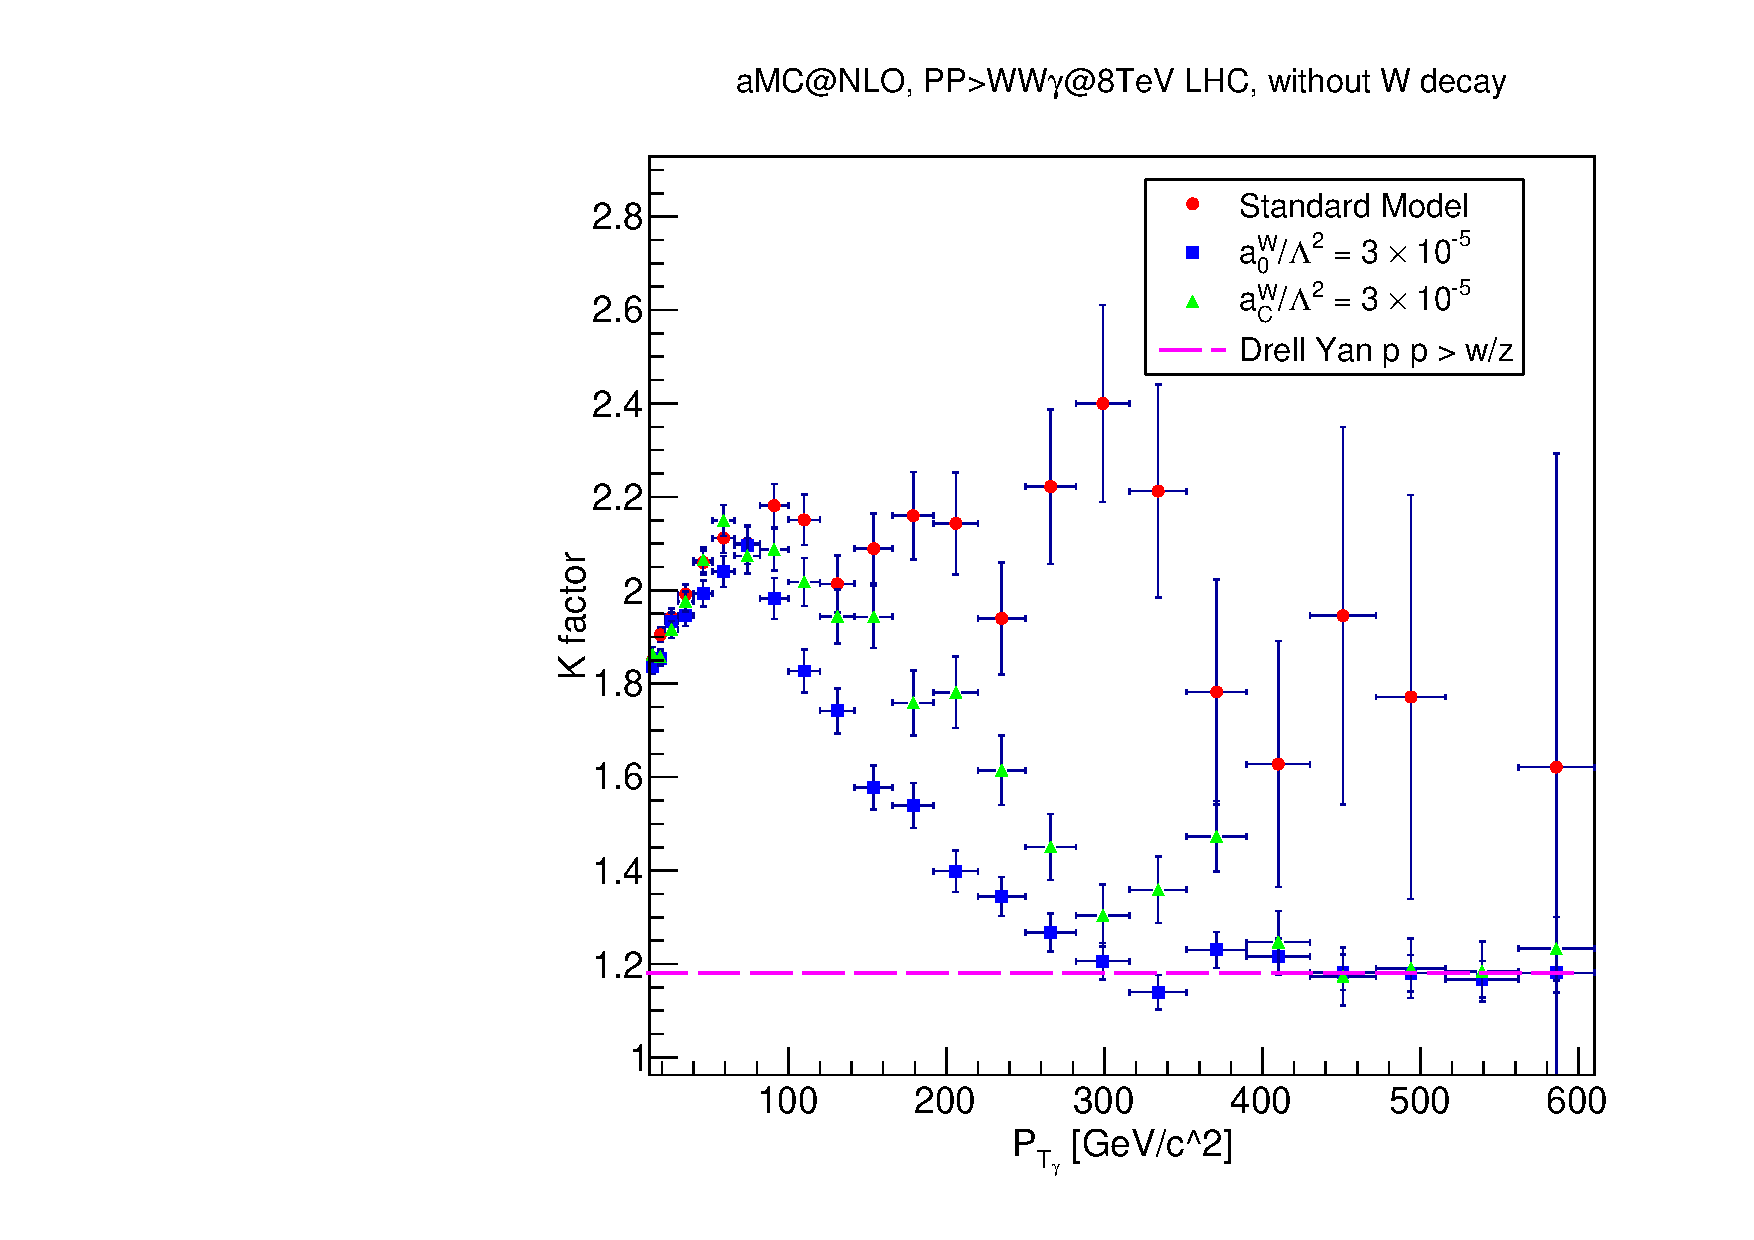
\includegraphics[width=0.4\textwidth]{figs/kAwwa_pt.pdf}
\caption{\label{k-Awwa} \wwa signal aQGC sample K-factor distribution as a function of $p_{T_{\gamma}}$}}
\end{figure}

\begin{figure}[]{
\centering
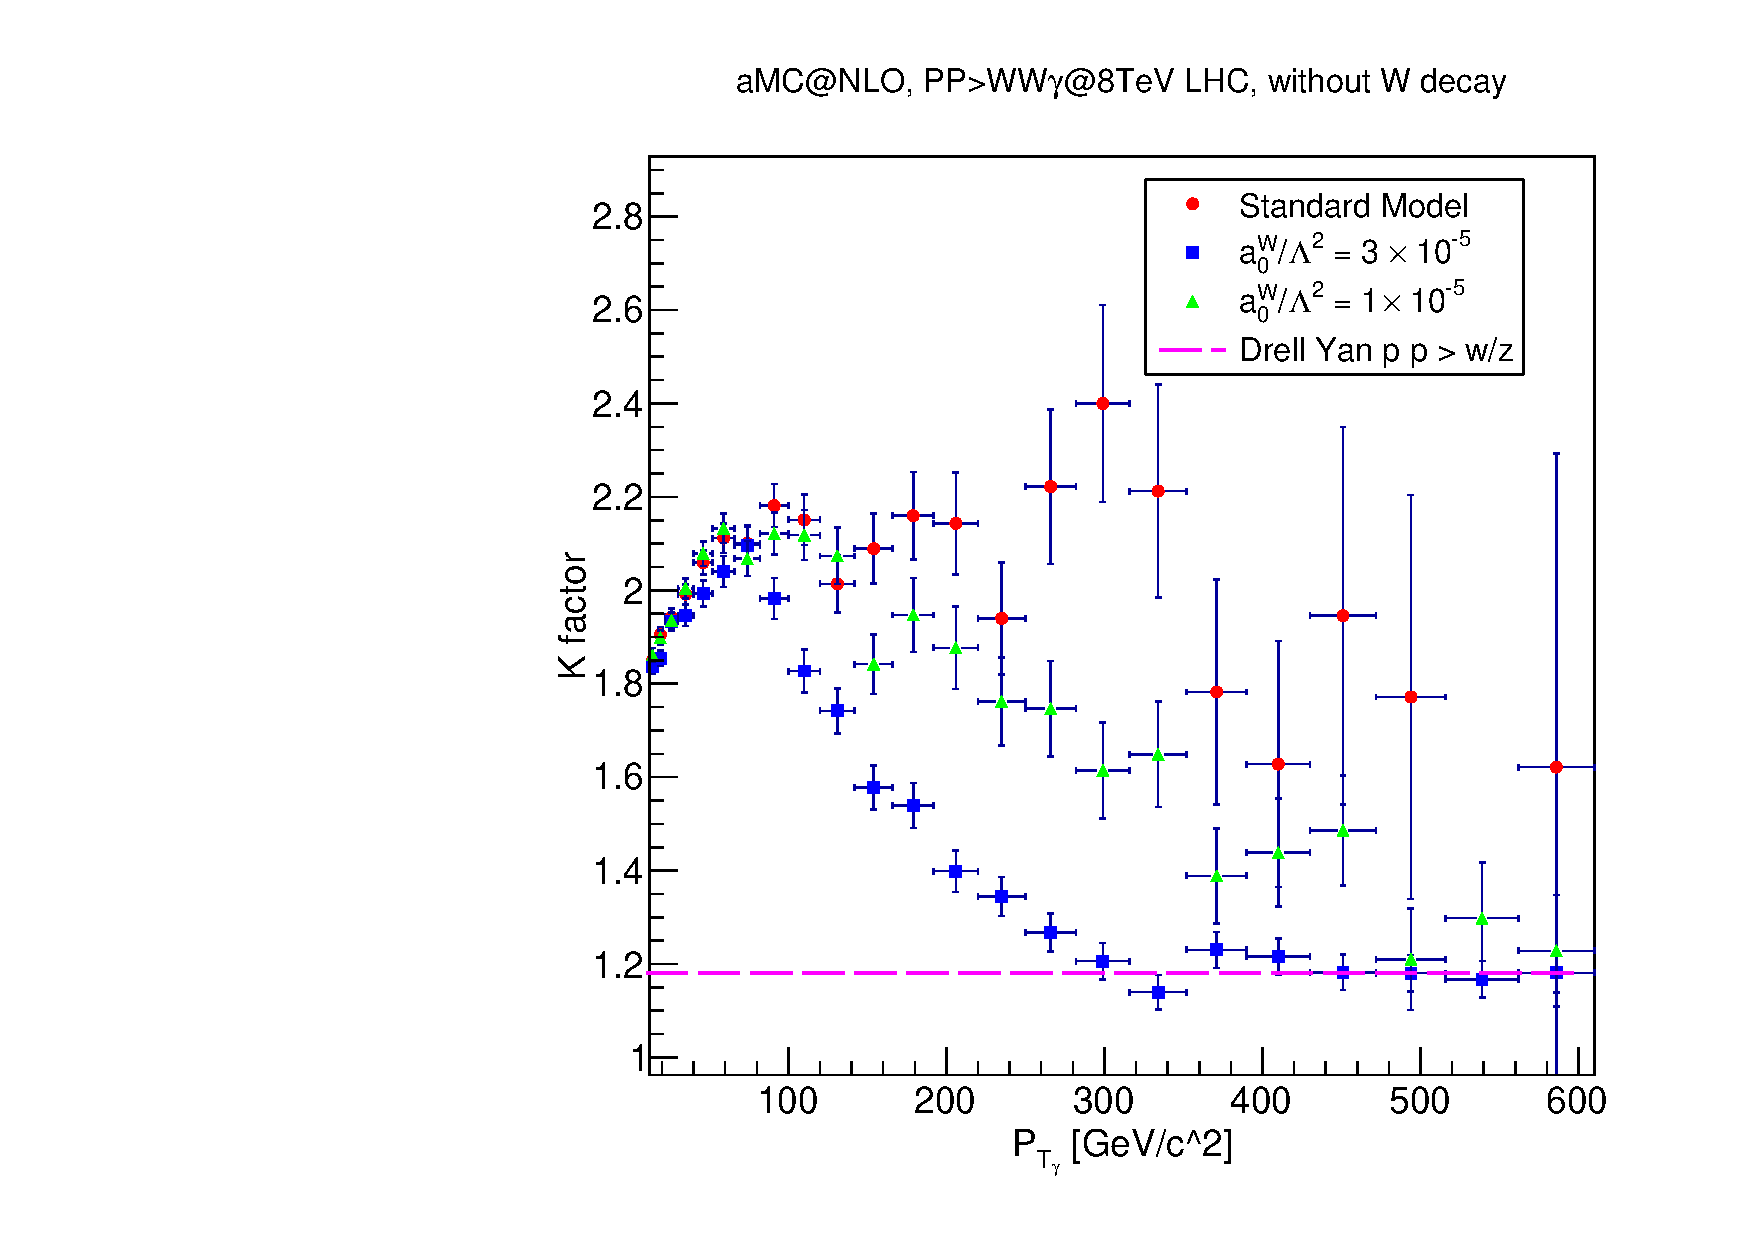
\includegraphics[width=0.4\textwidth]{figs/diffvalue_Kfactor.pdf}
\caption{\label{k-diffvalue} \wwa signal aQGC sample K-factor distribution with different $a_0^W/\Lambda^2$ values }}
\end{figure}

\begin{figure}[]{
\centering
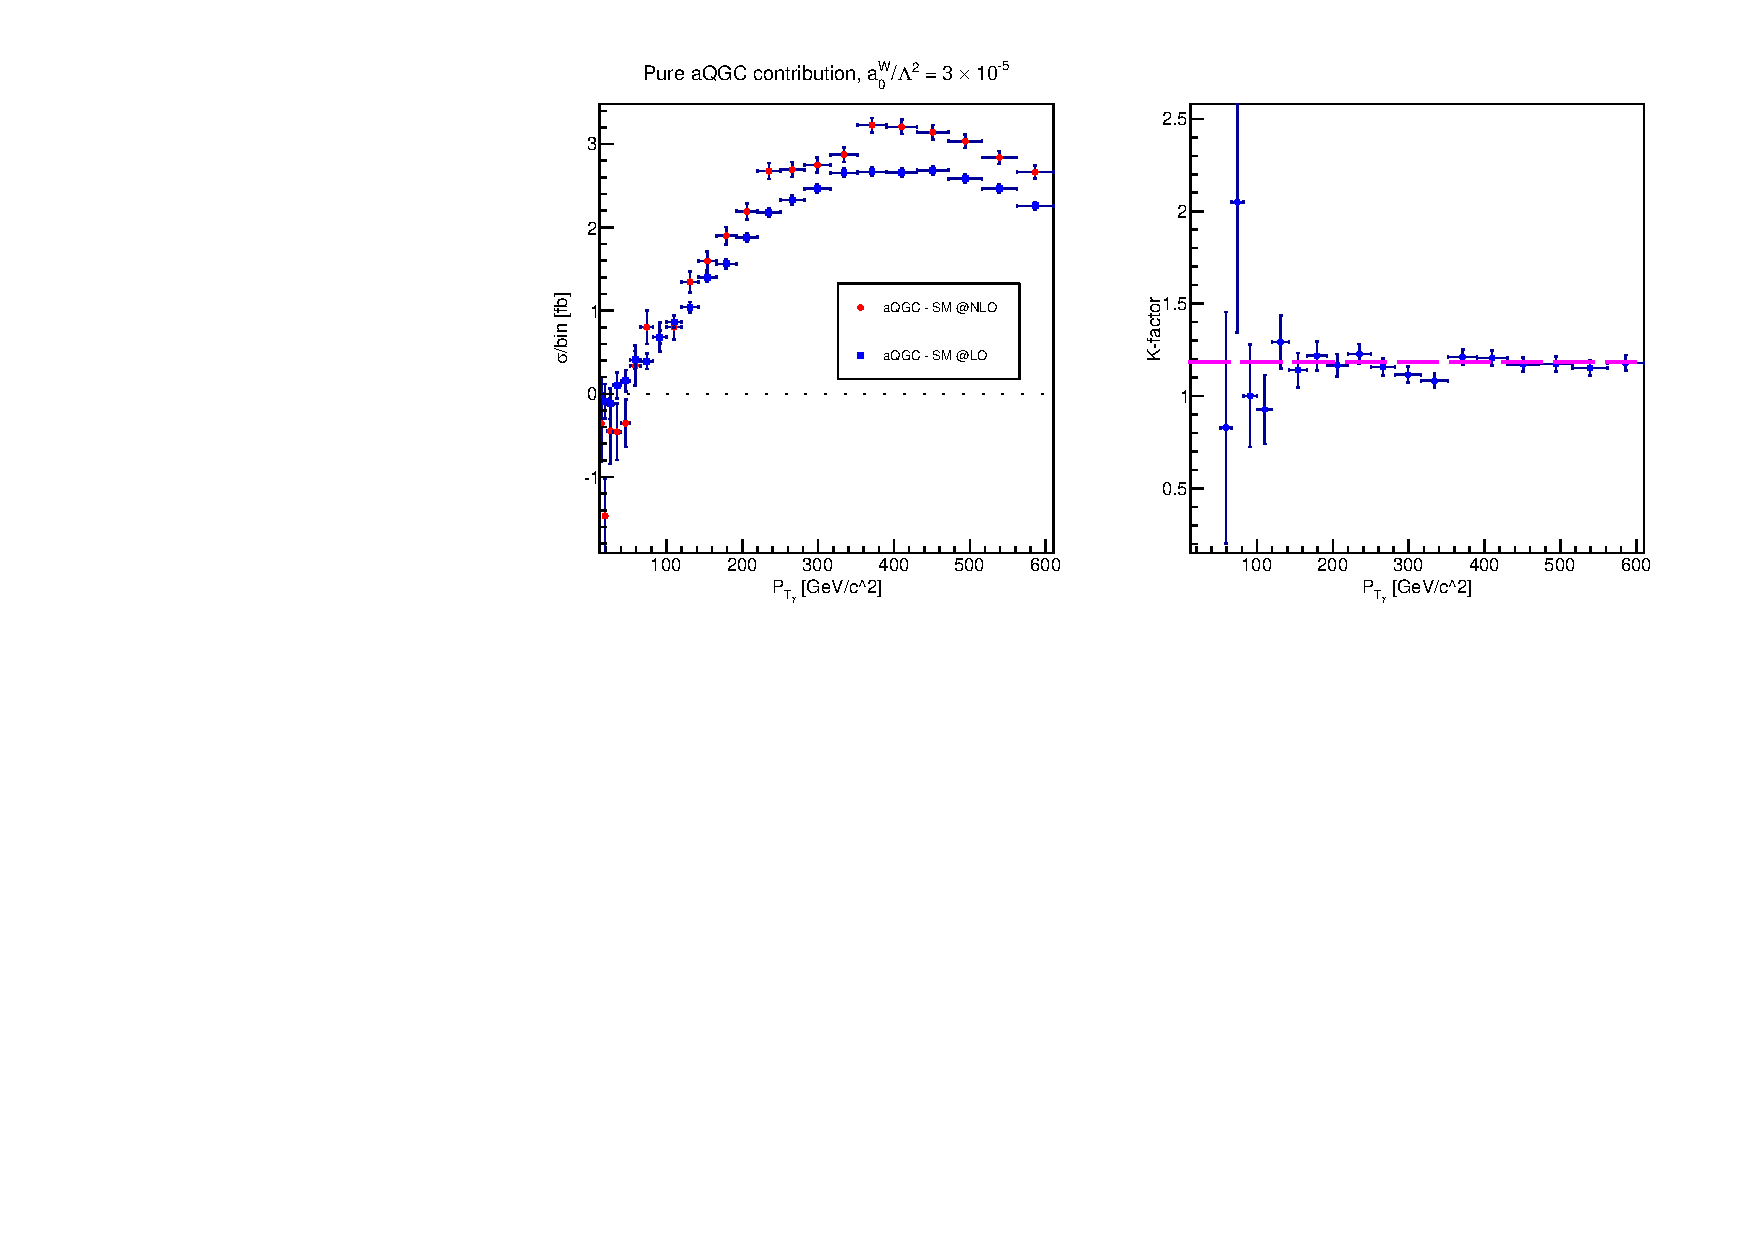
\includegraphics[width=0.8\textwidth]{figs/pureaqgc_Kfactor.pdf}
\caption{\label{k-pureaqgc} \wwa signal aQGC-SM $p_{T_{\gamma}}$ distribution (left) and K factor distribution (right), with $a_0^W/\Lambda^2 = 3 \times 10^{-5} GeV^{-2}$}}
\end{figure}

As additional cross check we have calculated the K-factors for SM WV$\gamma$ with added aQGC for all values of the $a_0^W/\Lambda^2$ parameter and 
re-calculated the limits on this parameter. The limits are shown in Section~\ref{sec:aQGClim}, while the conclusion is that with either of the 
described two procedure we arrive to the same constrains on the aQGC values. Thus we have chosen to used the methods with constant Drell Yan like K-factor for 
aQGC-SM, as the precise calculation of the K-factors for all values of all studied aQGC parameter will take vary long time.
In this last cross check we have used the following function to fit the K-factor shape for SM WV$\gamma$ with added aQGC:
\begin{equation}
\begin{cases}
slp \cdot x + ( top - slp \cdot cuta), \text{     } x \leq cuta  \\
(top-1.185) \cdot exp(-tau \cdot (x-cuta)) + 1.185, \text{     } x > cuta 
\end{cases}
\label{k-fitfunc}
\end{equation}
where the slp, top, cuta, tau are fit parameters and x represent the $p_{T_{\gamma}}$. K-factors and the fit are shown on  
Figure~\ref{k-fitshape} for $a_0^W/\Lambda^2 = p \times 10^{-5} GeV^{-2}$, where $p= 2,3,5.


\begin{figure}[]{
\centering
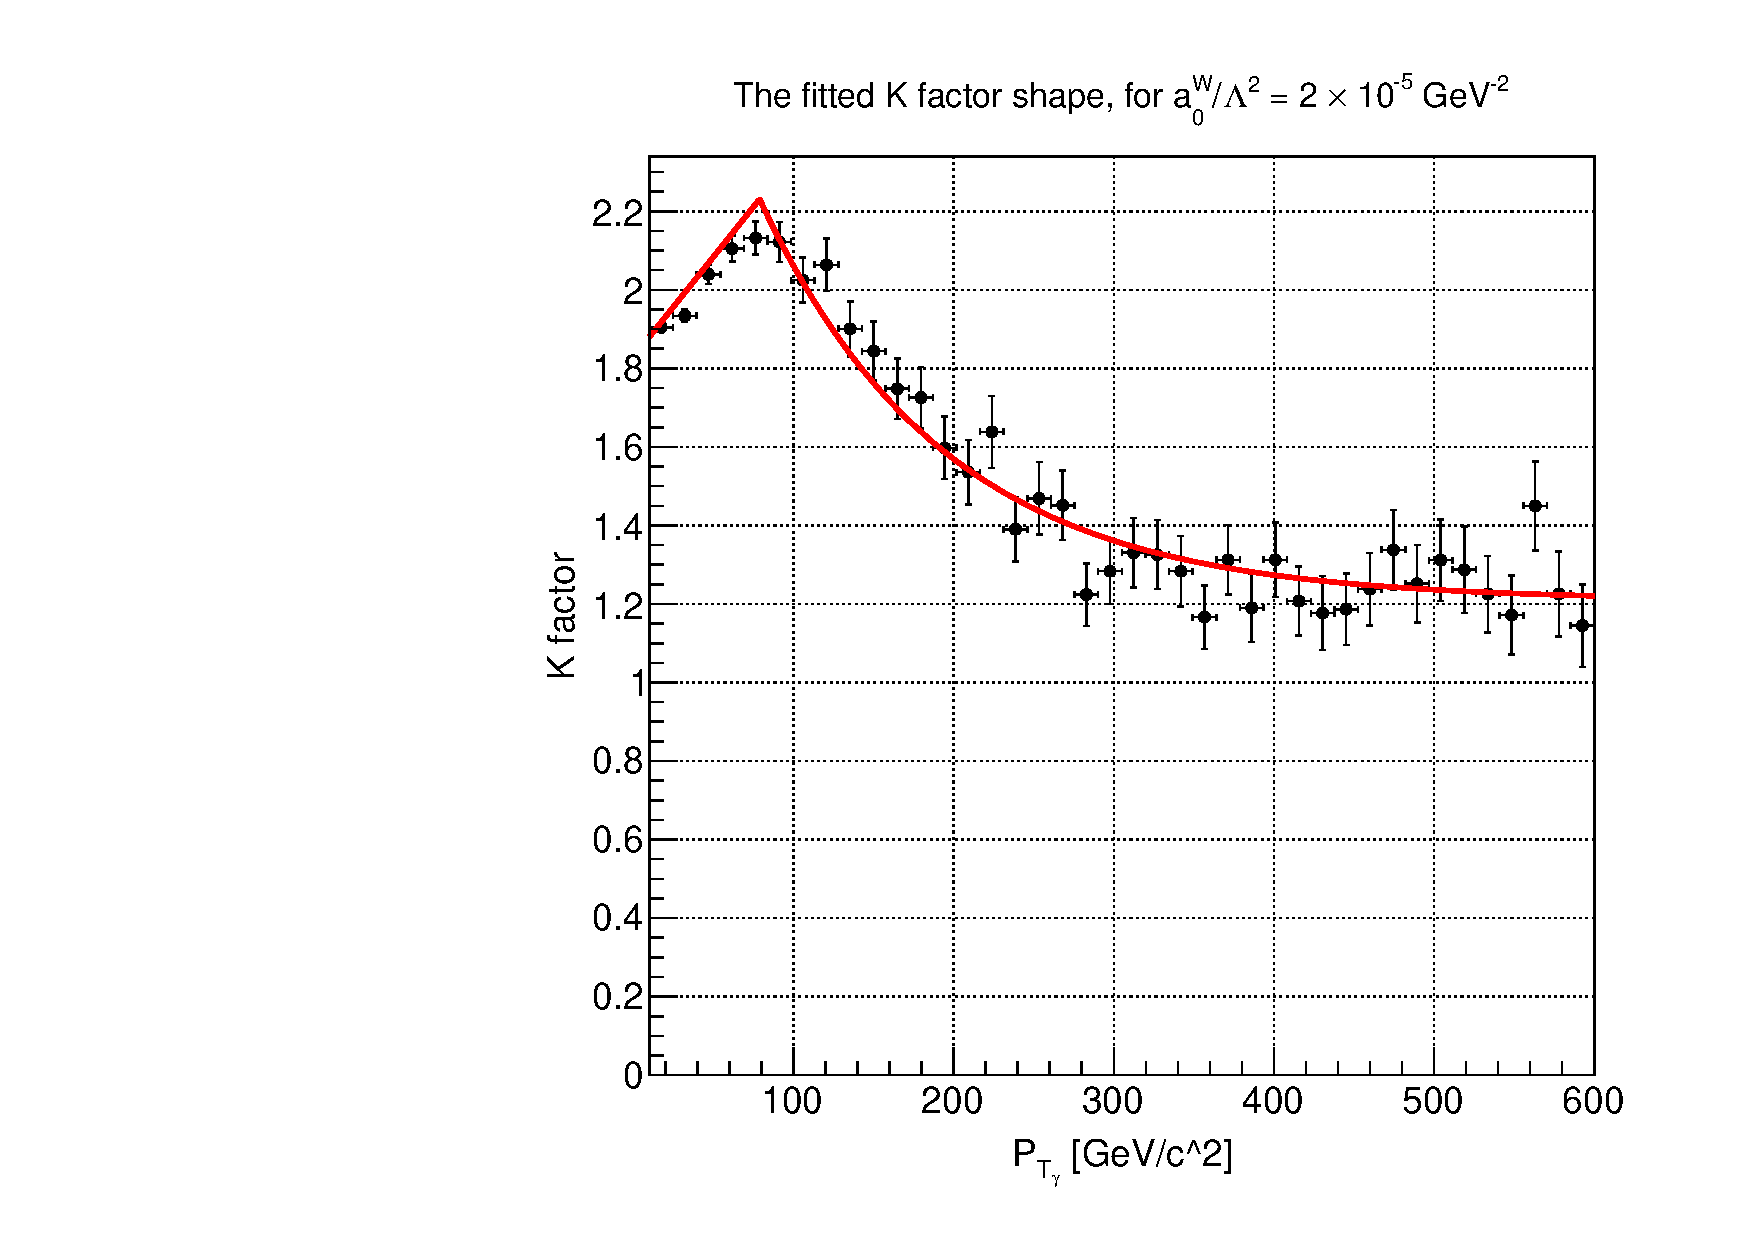
\includegraphics[width=0.4\textwidth]{figs/a0w_kshape_p2.pdf}
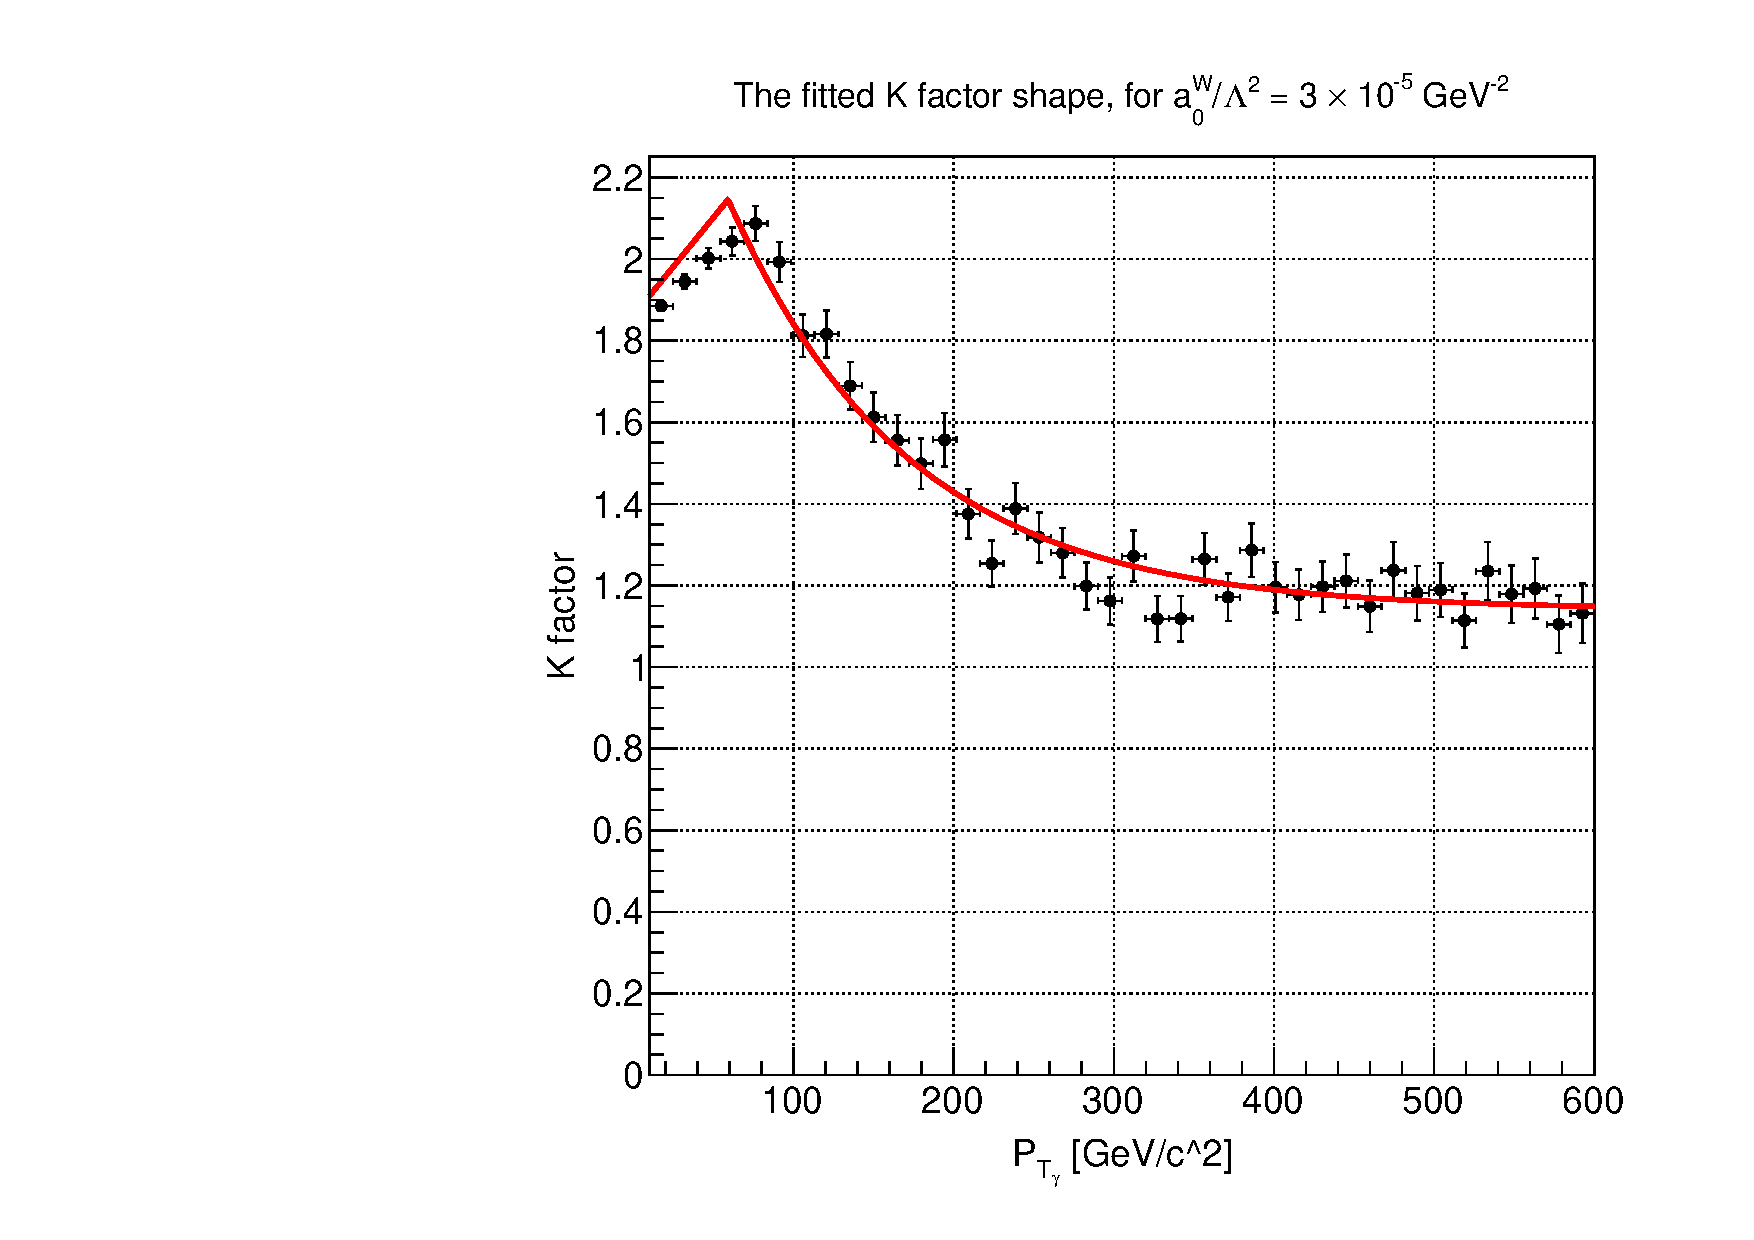
\includegraphics[width=0.4\textwidth]{figs/a0w_kshape_p3.pdf}
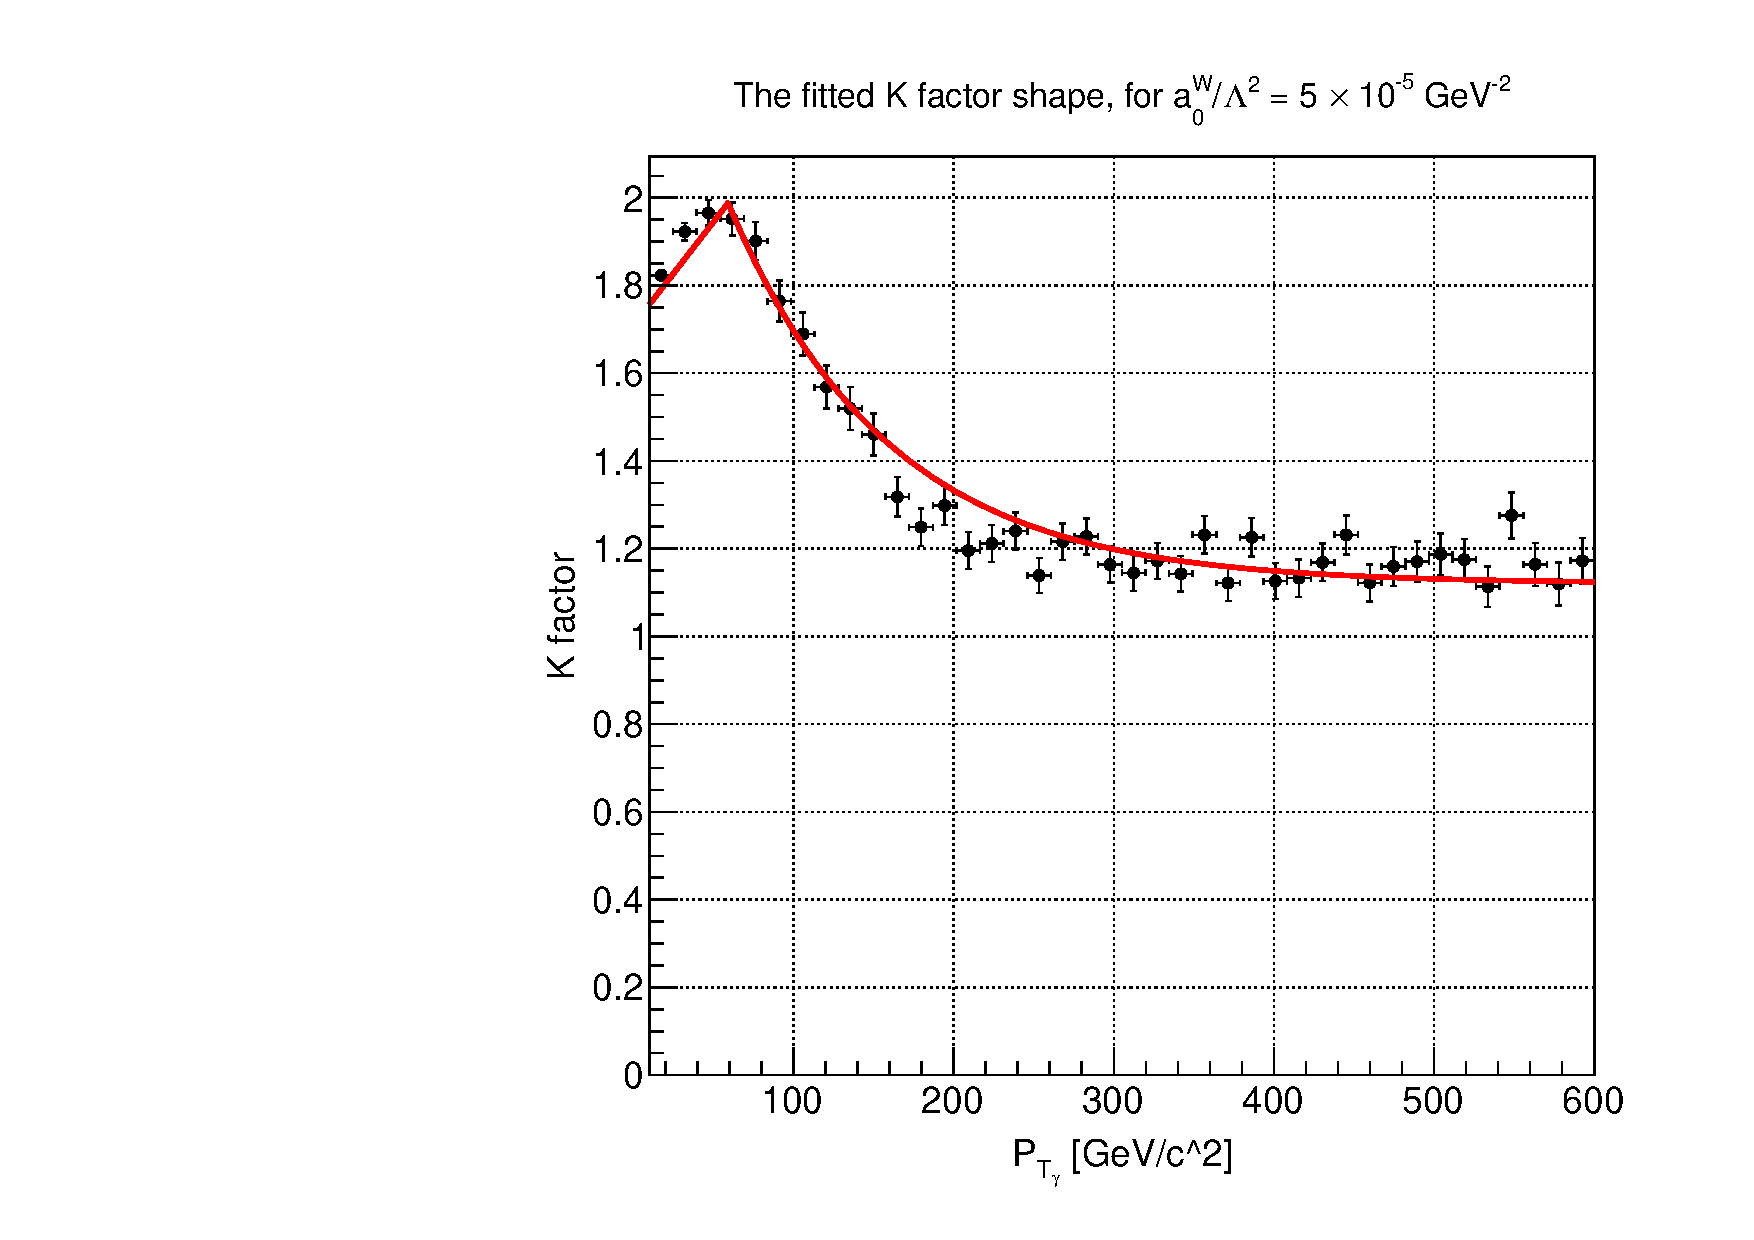
\includegraphics[width=0.4\textwidth]{figs/a0w_kshape_p5.pdf}
%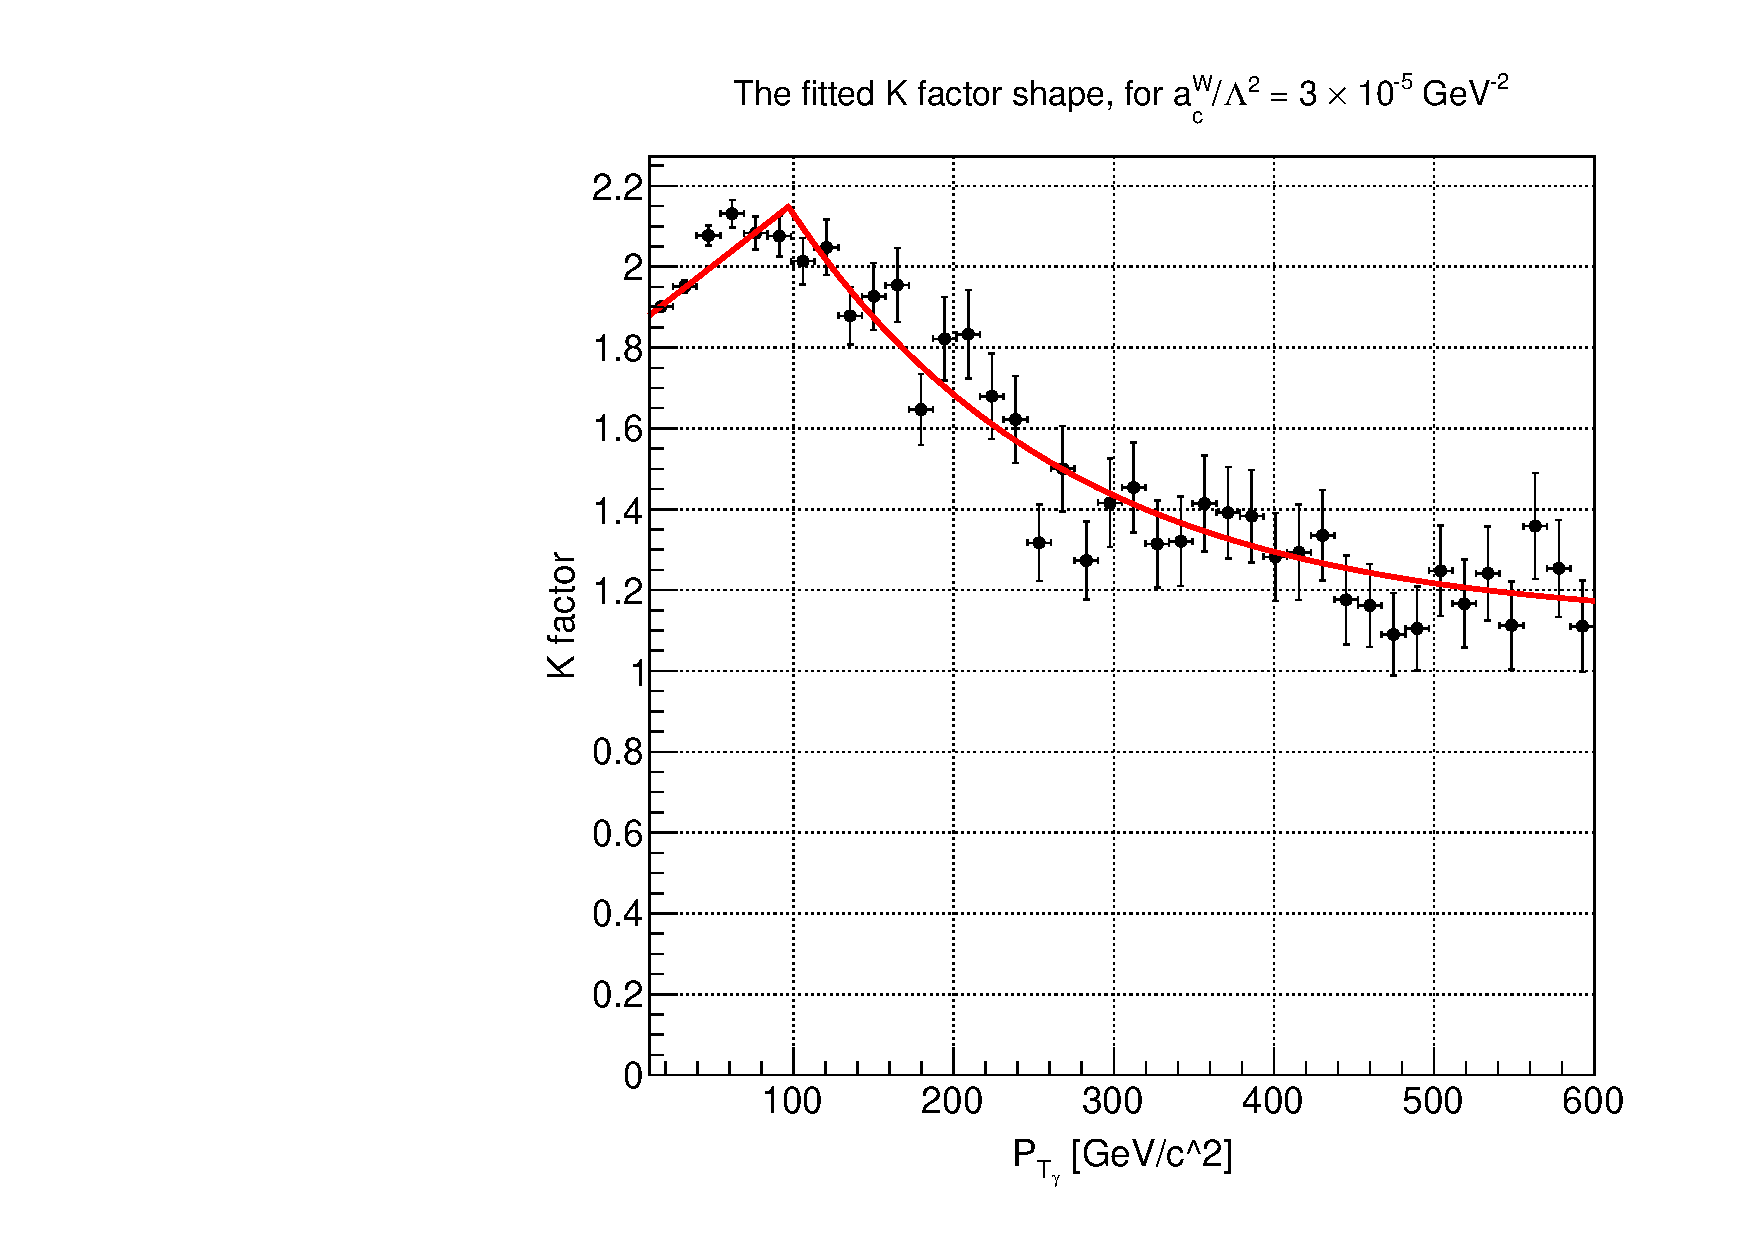
\includegraphics[width=0.4\textwidth]{figs/acw_kshape.pdf}
\caption{\label{k-fitshape} K factor shape fitted with function ~\ref{k-fitfunc}, for $a_0^W/\Lambda^2 = 2,3,5 \times 10^{-5} GeV^{-2}$  }}
\end{figure}


\subsection{W$\gamma$ + jets background estimation}

In order to estimate the normalization of the major background
W$\gamma$+jets, we used a data-driven technique.
%% The method involved analyzing sideband distributions in the W$\to$jj
%% mass spectrum in data.
%% These sidebands lie outside of a 70-100 GeV $M_{W,Z}$ window,
%% and in addition include all other normalized Monte Carlo background
%% and signal contributions, of which there was less than 0.6\% signal
%% contamination.
The background normalization in the signal region is extracted with a
binned maximum likelihood fit to the dijet invariant mass
distribution $m_{jj}$ of the two leading jets. The signal region
corresponding to the W and Z mass windows, $70 GeV < m_{jj} <
100 GeV$, is excluded from the fit.  The W$\gamma$+jets shape is
taken from simulation.  The overall normalizations of the
W$\gamma$+jets and fake photon components are allowed to vary in the
fit.  All other backgrounds, which contribute less than 10\% to the
total, are based on simulation and are fixed to their SM expectations
with uncertainties.  The multi-jet background shape is derived from
data by relaxing lepton isolation and identification requirements. Its
contribution to the total number of events is evaluated from a
separate two-component likelihood fit to the \MET
distribution, and fixed in the $m_{jj}$ fit according to this
fraction within uncertainties~(\cite{CMS-AN-12-224}, Section 11).
Normalization for the W$\gamma$+jets is measured to be $1.099 \pm
0.073$ for muons and $1.074 \pm 0.085$ for electrons. The quality of
the fit is illustrated on Figure ~\ref{fig:wapjets_kfct}

Table~\ref{tab:MCxsec} summarizes
the K-factors and cross sections used for each Monte Carlo sample,
as well as the treatment of all backgrounds in the fit.

\begin{table}[htb]
\centering
\scalebox{0.8}{
  \begin{tabular}{|l|c|c|l|}
  \hline
  MC Sample & K & $\sigma$ [pb] & External constraint on normalization \\
   &  &  & used in W$\gamma$+jets fit \\
  \hline
  \hline
  SM WW$\gamma$            & 2.1        & 0.02771    & Fixed \\
  SM WZ$\gamma$            & 2.1        & 0.00578008 & Fixed \\
  anomalous WWV$\gamma$    & 1.185      & -          & NA    \\
  W$\gamma$+jets           & 1.10(mu),1.07(el)  & 9.37246    & Unconstrained \\
  Fake photon              & from data  & -          & Constrained \\
  Multi-jet                & from data  & -          & Fixed: \MET fit in data $\pm$ 50\% (100\%) for electrons (muons) \\
  Z$\gamma$+jets           & 1          & 0.63196    & Fixed \\
  t$\overline{t}\gamma$    & 1          & 1.44       & Fixed \\
  Single Top (s-channel)   & NLO        & 3.89394    & Fixed \\
  Single Top (t-channel)   & NLO        & 55.531     & Fixed \\
  Single Top (tw-channel)  & NLO        & 11.1773    & Fixed \\
  Single Top (ps-channel)  & NLO        & 1.75776    & Fixed \\
  Single Top (pt-channel)  & NLO        & 30.0042    & Fixed \\
  Single Top (ptw-channel) & NLO        & 11.1773    & Fixed \\
  \hline
  \end{tabular}}
  \caption{List of backgrounds, the theoretical K-factors and cross
  sections used for MC-based backgrounds, and how they are treated in
  the background normalization template fit. The data-driven K-factor
  for W$\gamma$+jets sample is listed for both the muon and electron
  channels.}  \label{tab:MCxsec}
\end{table}

%% Examples of the $m_{jj}$ fit are shown in
%% Figure~\ref{fig:mjj_mH350} for the muon channel, with selections
%% optimized for Higgs mass hypotheses 190\GeVnn, 300\GeVnn, and
%% 500\GeVnn. The uncertainties in the normalization obtained from the
%% fit are propagated to the limit calculation as a systematic
%% uncertainty.  The signal $m_{jj}$ distributions are shown in
%% figure~\ref{fig:mjj_signals}.

\begin{figure}[b]
   \begin{center}
      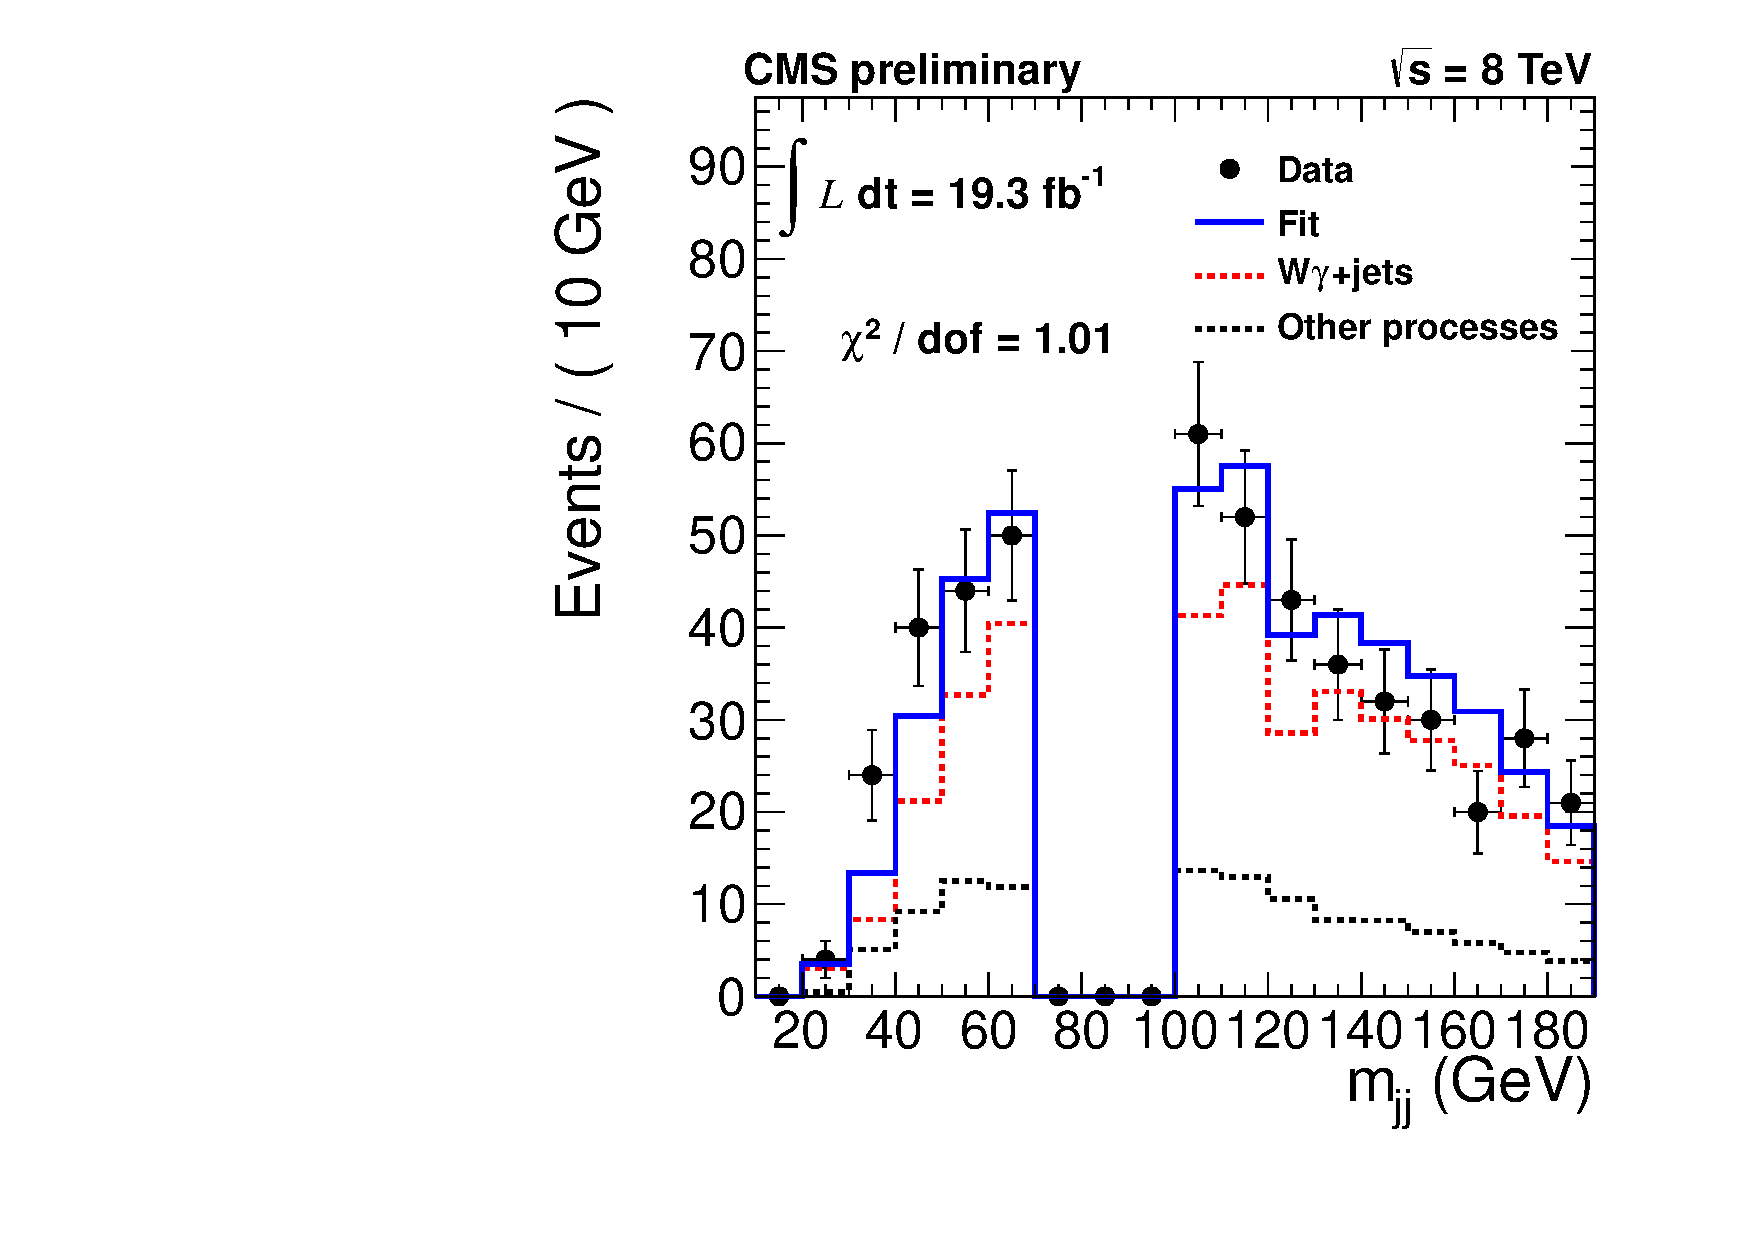
\includegraphics[width=0.4\textwidth]{figs/mu_mjj1.pdf}
      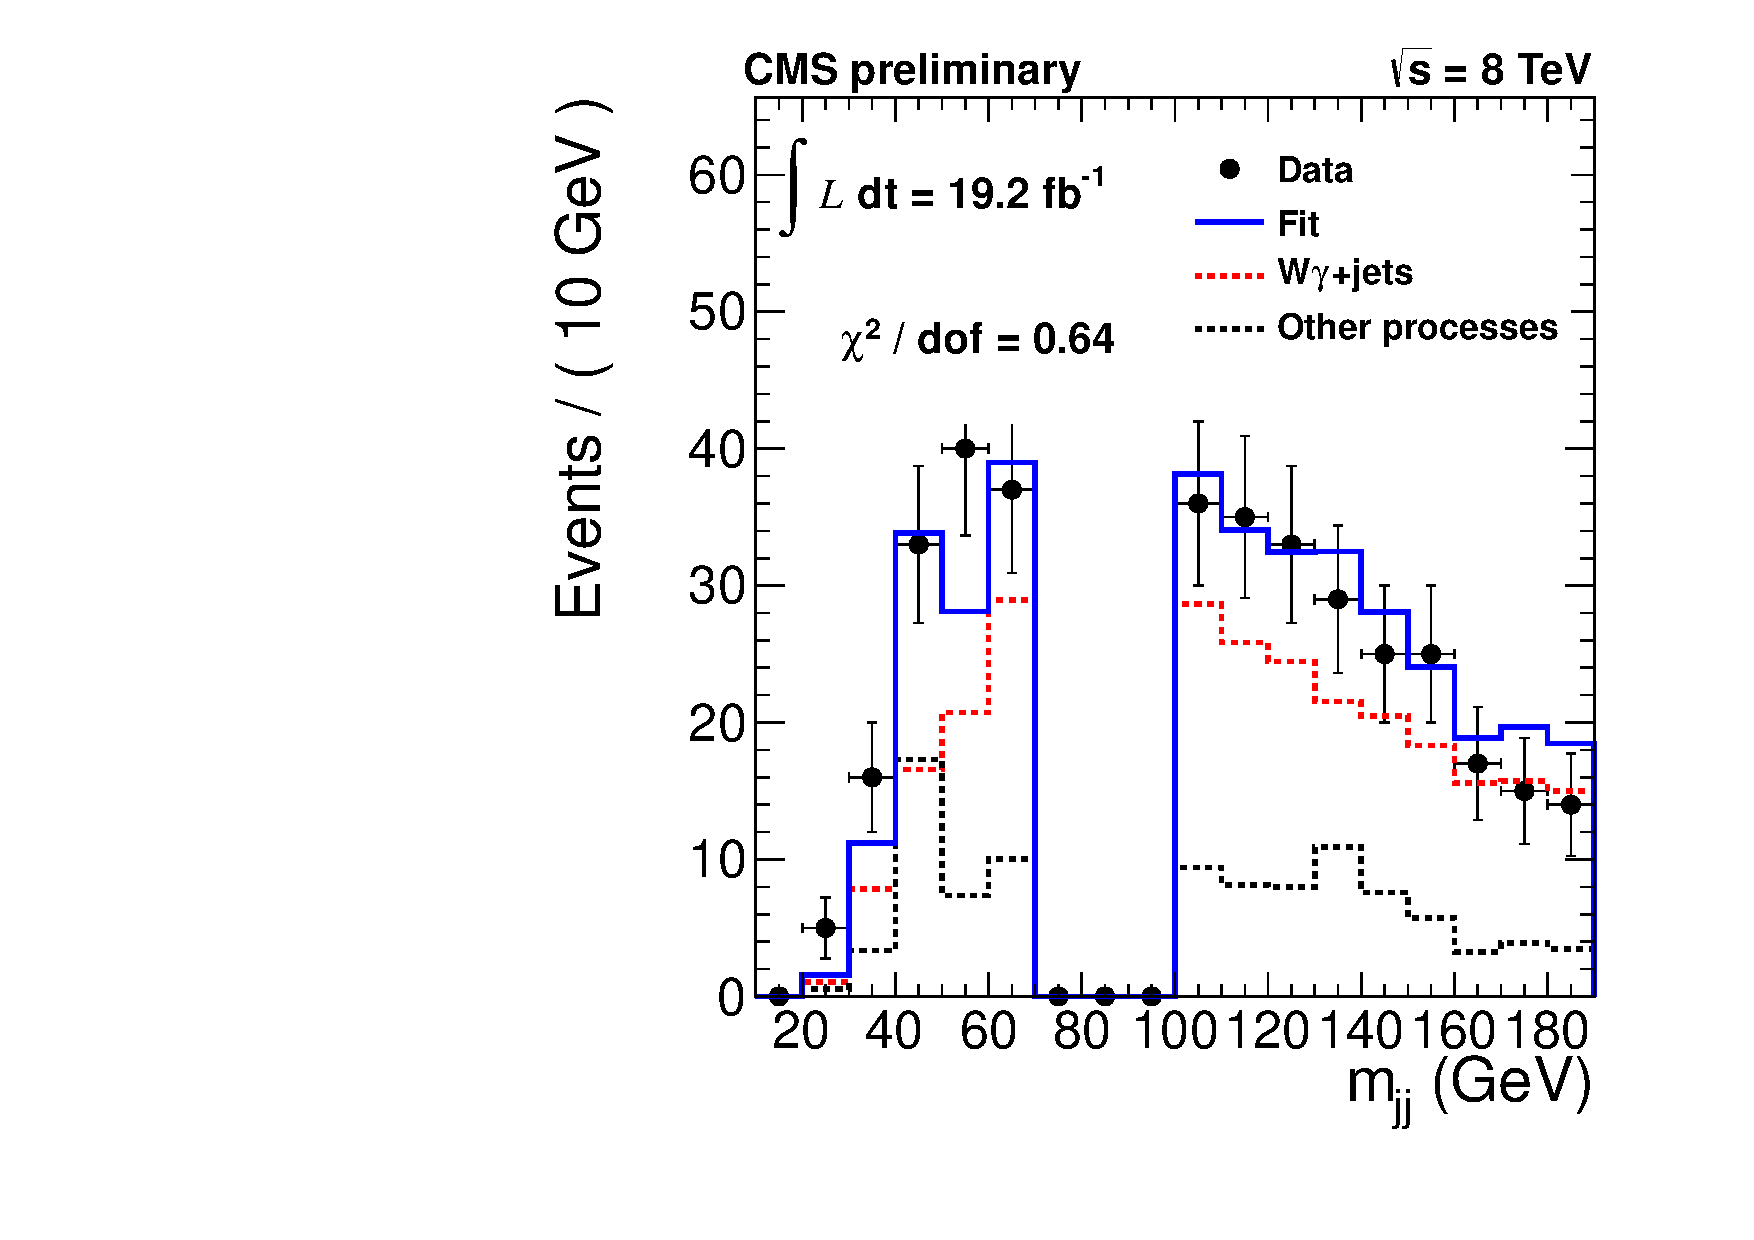
\includegraphics[width=0.4\textwidth]{figs/el_mjj1.pdf}
      \caption{Data and MC dijet mass sidebands used to estimate the data-driven W$\gamma$+jets K-factor.}
      \label{fig:wapjets_kfct}
   \end{center}
\end{figure}



%%%%%%%%%%%%%%%%%%%%%%%%%%%%%%%%%%%%%%%%%%%%%%%%%%%%%%%%%%%%%%%%%%%%%%%%%%
%%%%%%%%%%%%%%%%%%%%%%%%%%%%%%%%%%%%%%%%%%%%%%%%%%%%%%%%%%%%%%%%%%%%%%%%%%
\clearpage{}
\section{Signal and background expectations from CMS simulation}
\label{sec:MCexpectations}
% ---- ---- ---- ---- ---- ---- ---- ---- ---- ---- --

In order to compare the Monte Carlo processes with observed data, we first normalize each sample to the observed integrated luminosity for both the muon and electron channel of the full 2012 dataset, which, after single lepton triggers, is 19.297 $\textnormal{fb}^{-1}$ and 19.166 $\textnormal{fb}^{-1}$, respectively.  To do this, we use the following calculation

\begin{center}
\begin{equation}\label{normalize}
N_{events} = K \cdot \sigma \cdot \cal{L} \cdot \cal{A} \cdot \varepsilon_{MC} \cdot SF
\end{equation}
\end{center}

where $N_{events}$ is the expected event yield for each Monte Carlo
process after event selection, $K$ is the NLO:LO K-factor, $\sigma$ is
the theoretical cross section for each Monte Carlo process, $\cal{L}$
is the observed integrated luminosity, $\cal{A} \cdot
\varepsilon_{MC}$ is the Monte Carlo process's acceptance times event
selection efficiency, and SF is the efficiency scale factor for data
and Monte Carlo ($\frac{\varepsilon_{data}}{\varepsilon_{MC}}$).

We use the functional fit to the photon fake rate discussed in section~\ref{sec:photon} to estimate the number of observed data events that are from the photon-faking jet background.  
%Since the fit was applied to the fake ratio, or $\frac{fake photon candidates}{true photon candidates}$, then after algebraic reordering the photon $p_{T}$-dependent fake rate function for the barrel region is described by

%\begin{center}
%\begin{equation}\label{fakerate}
%\frac{fake photon candidates}{all photon candidates} = [1 + (0.0345868 + \frac{1.44022 x 10^{4}}{p_{T}^{2.89994}})^{-1}]^{-1}
%\end{equation}
%\end{center}

%where the function can only be used for photon $p_{T}$ greater than 30 GeV.  We simply apply this function as a photon $p_{T}$-dependent scale factor to all observed data events that pass event selection cuts to estimate the fake photon contamination.  

Figures~\ref{photonplots}-\ref{eldijetplots} are Data and Monte Carlo comparison plots for various event kinematical distributions.

\begin{figure}[b]
\begin{center}
\subfigure[]{
   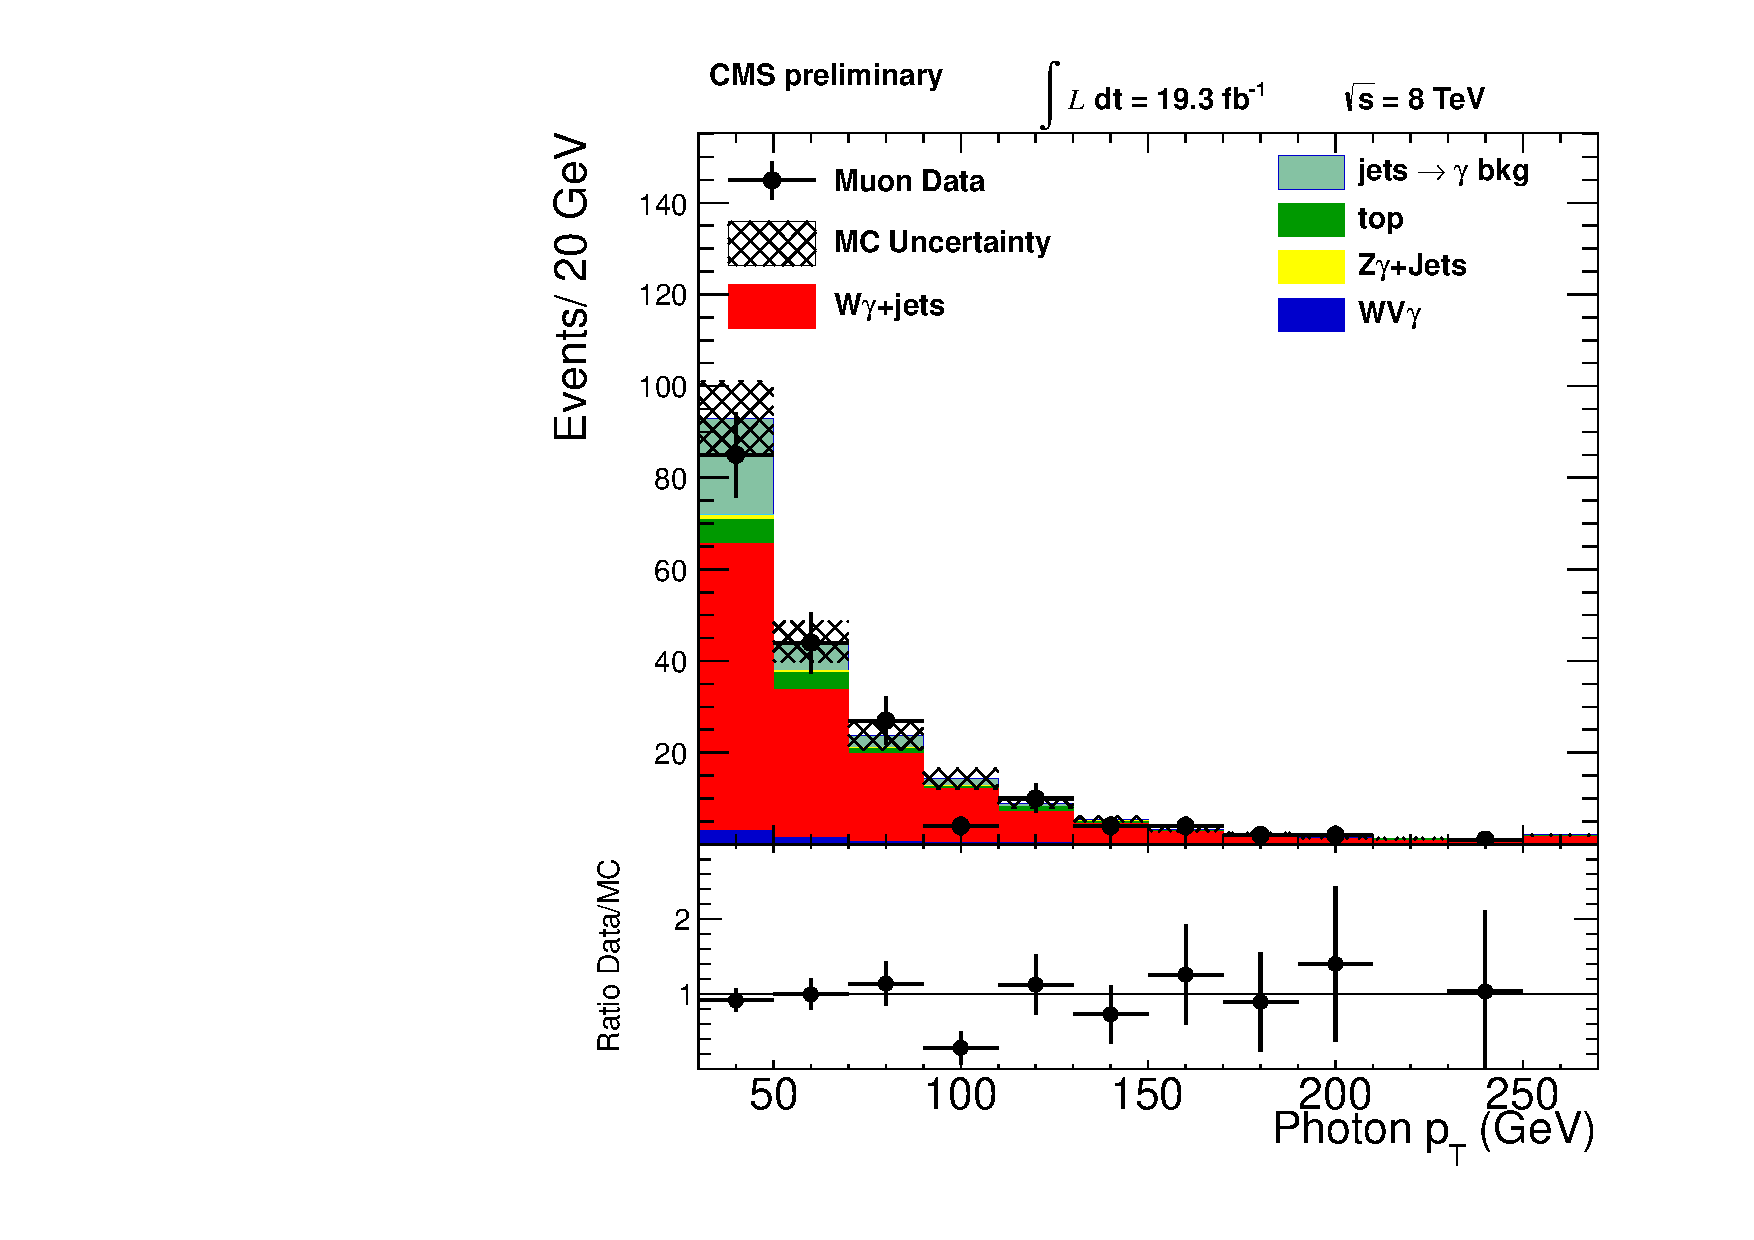
\includegraphics[width=.32\textwidth]{figs/mu_Photon_pt.pdf}
}
\subfigure[]{
   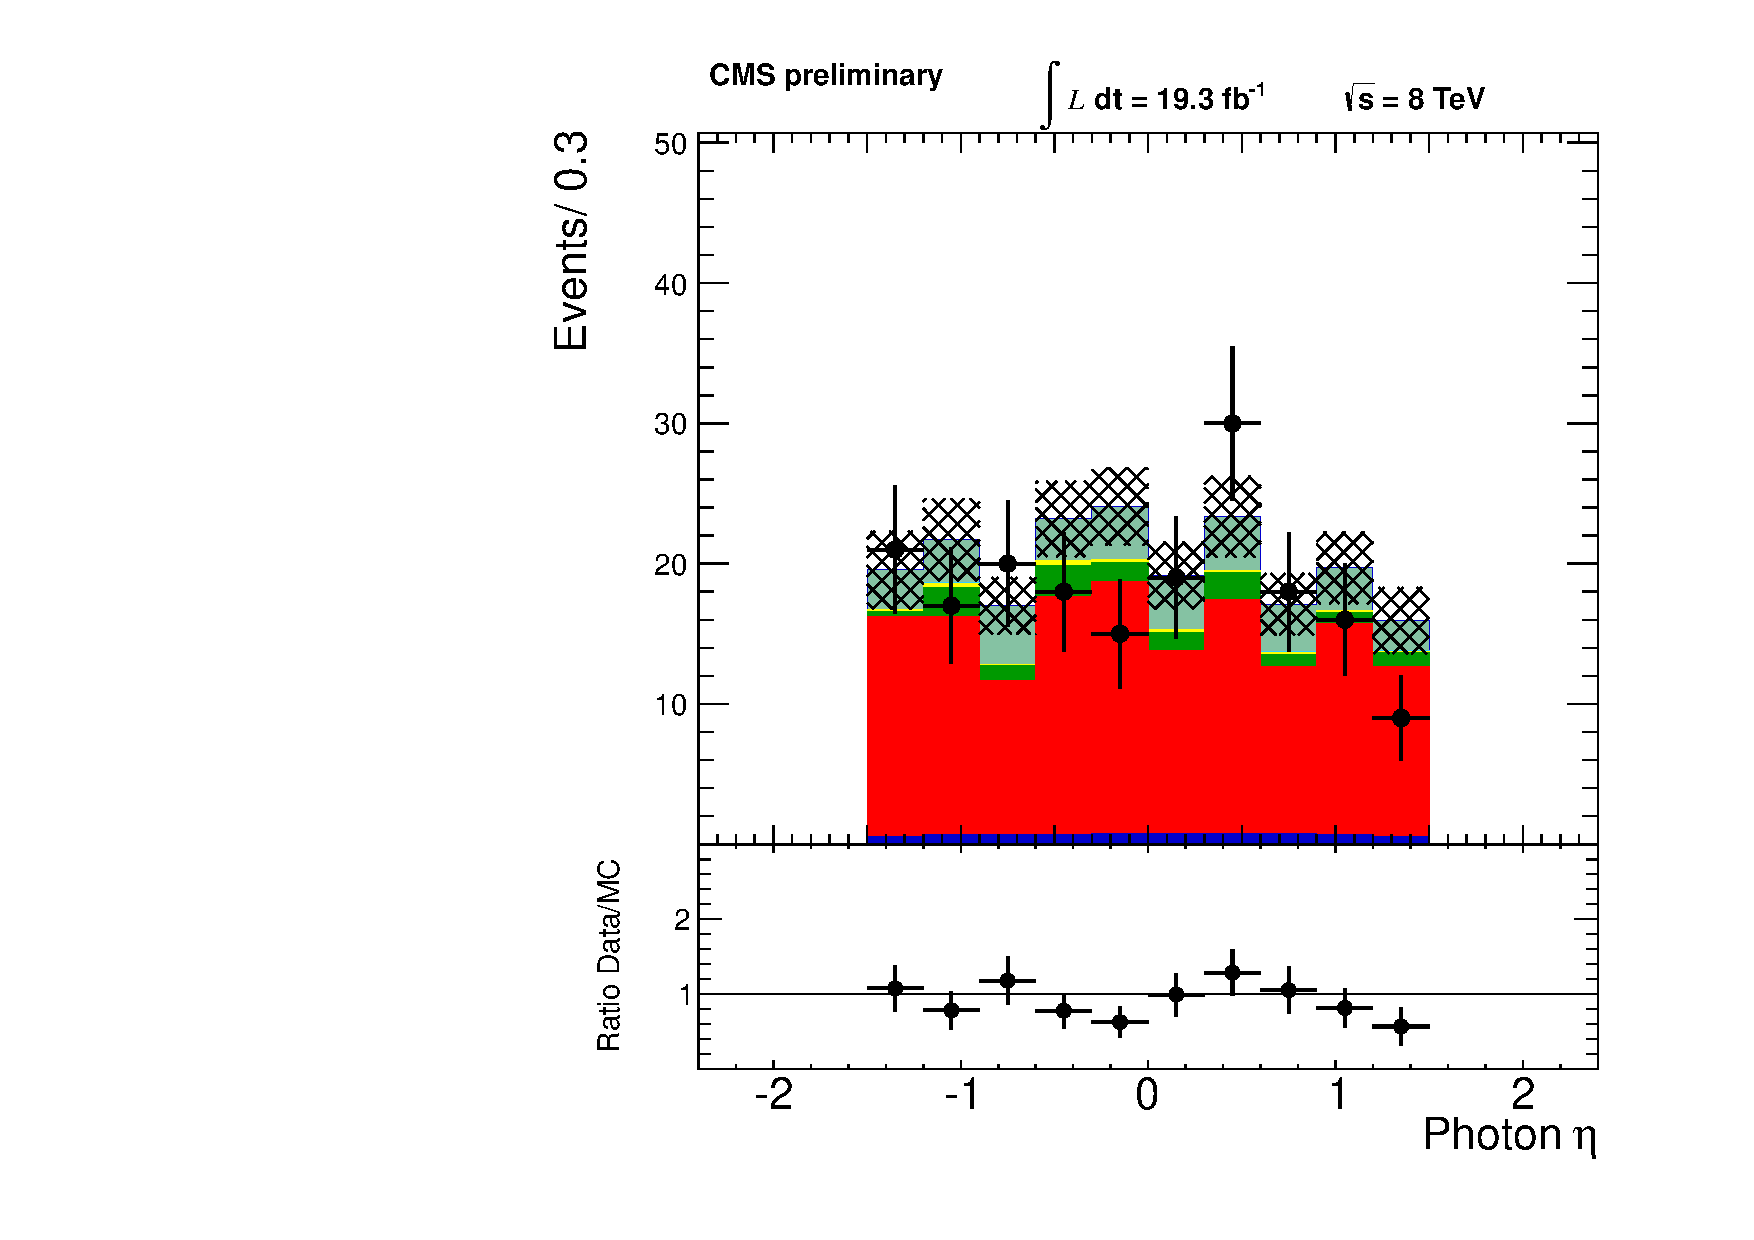
\includegraphics[width=.32\textwidth]{figs/mu_Photon_eta.pdf}
}
\subfigure[]{
   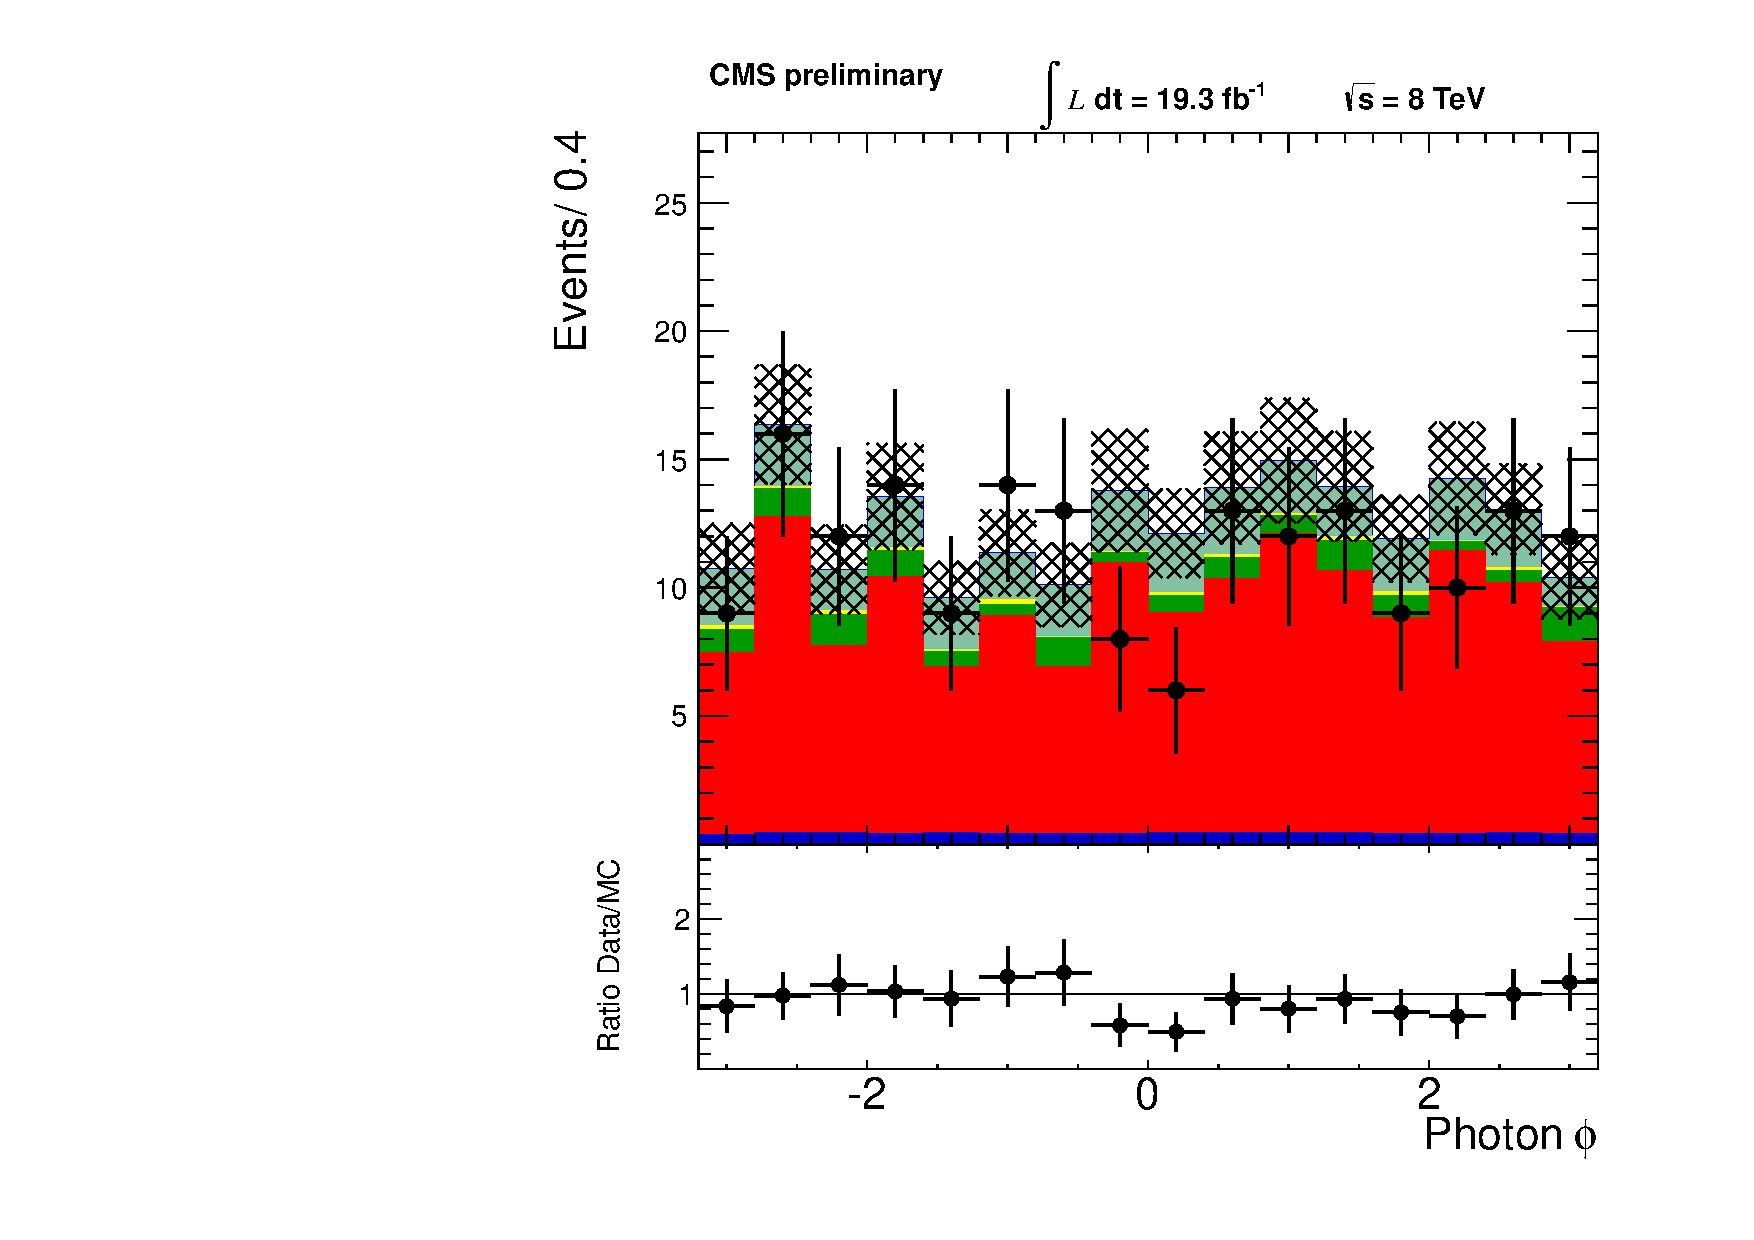
\includegraphics[width=.32\textwidth]{figs/mu_Photon_phi.pdf}
}\\
\subfigure[]{
   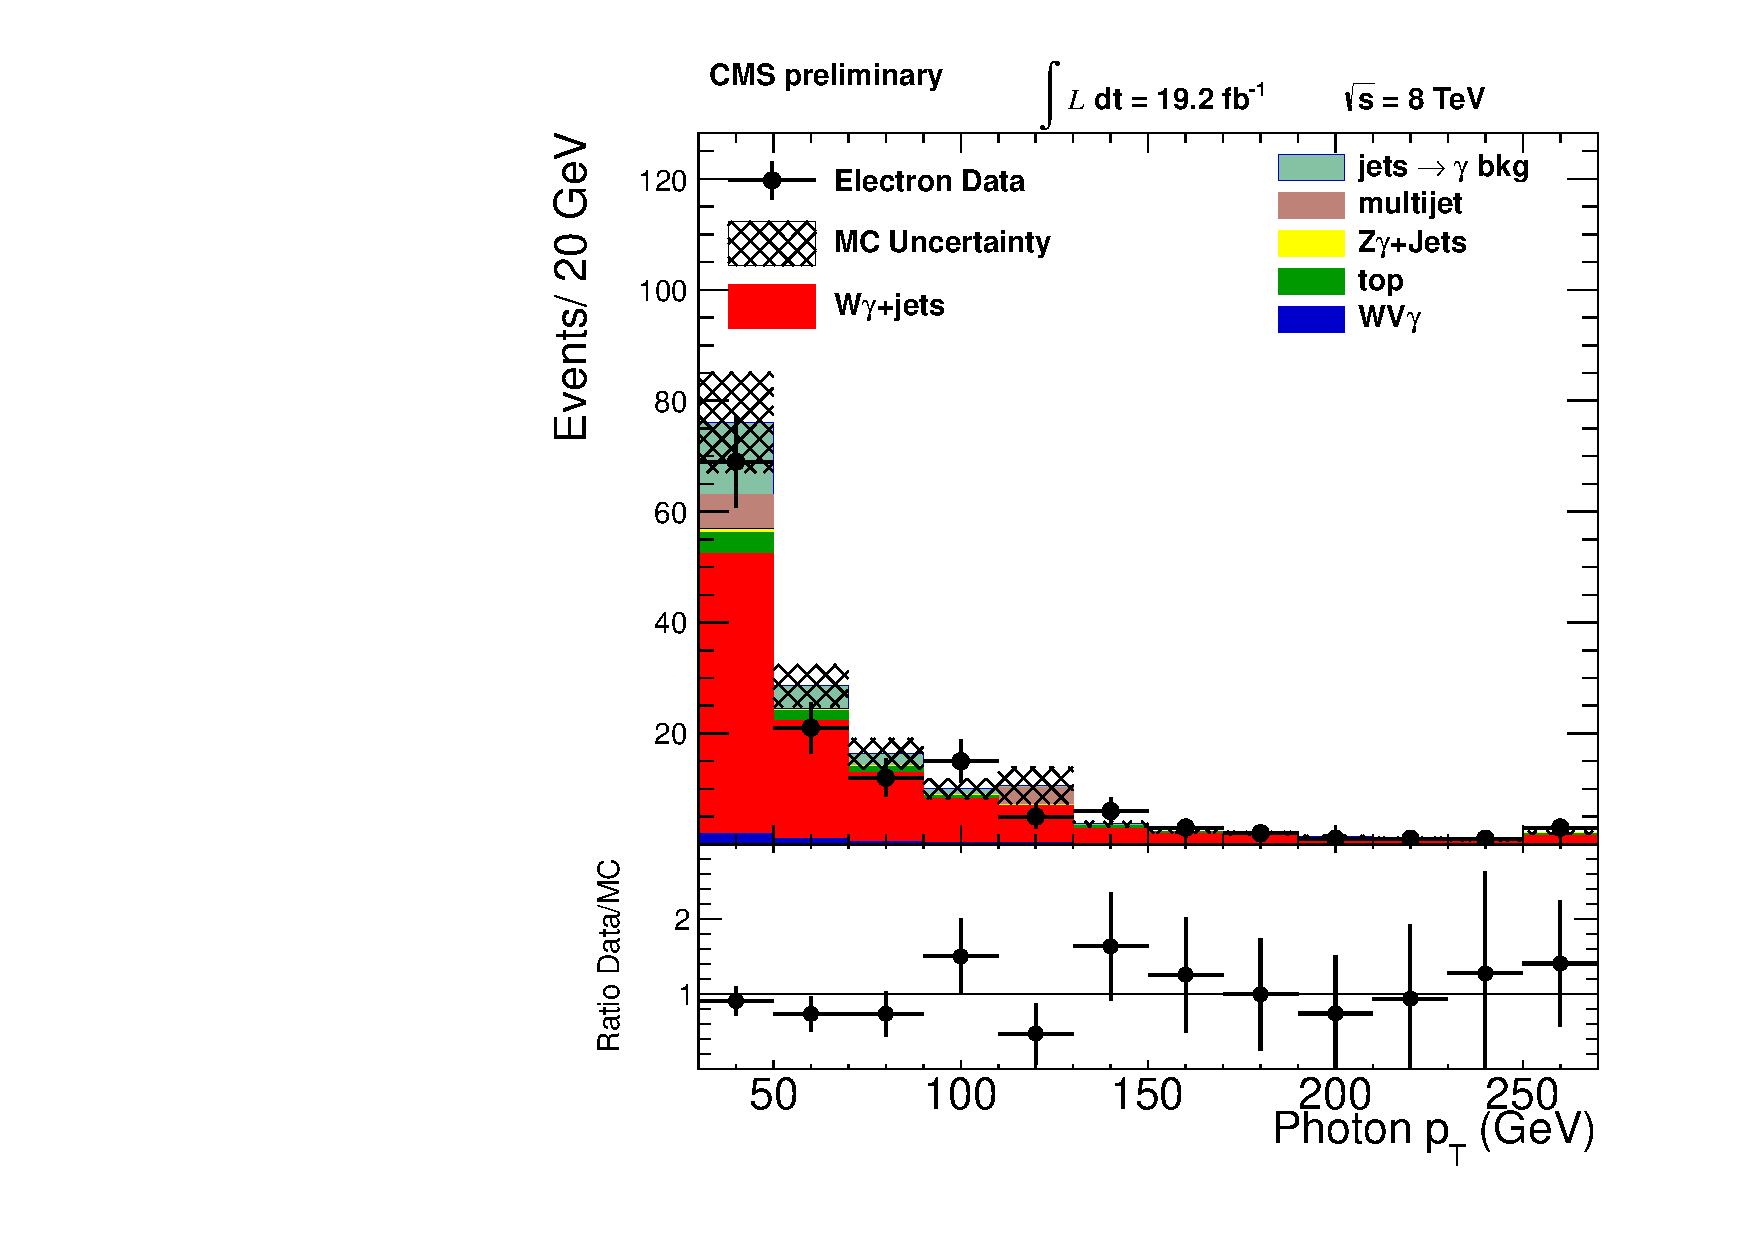
\includegraphics[width=.32\textwidth]{figs/el_Photon_pt.pdf}
}
\subfigure[]{
   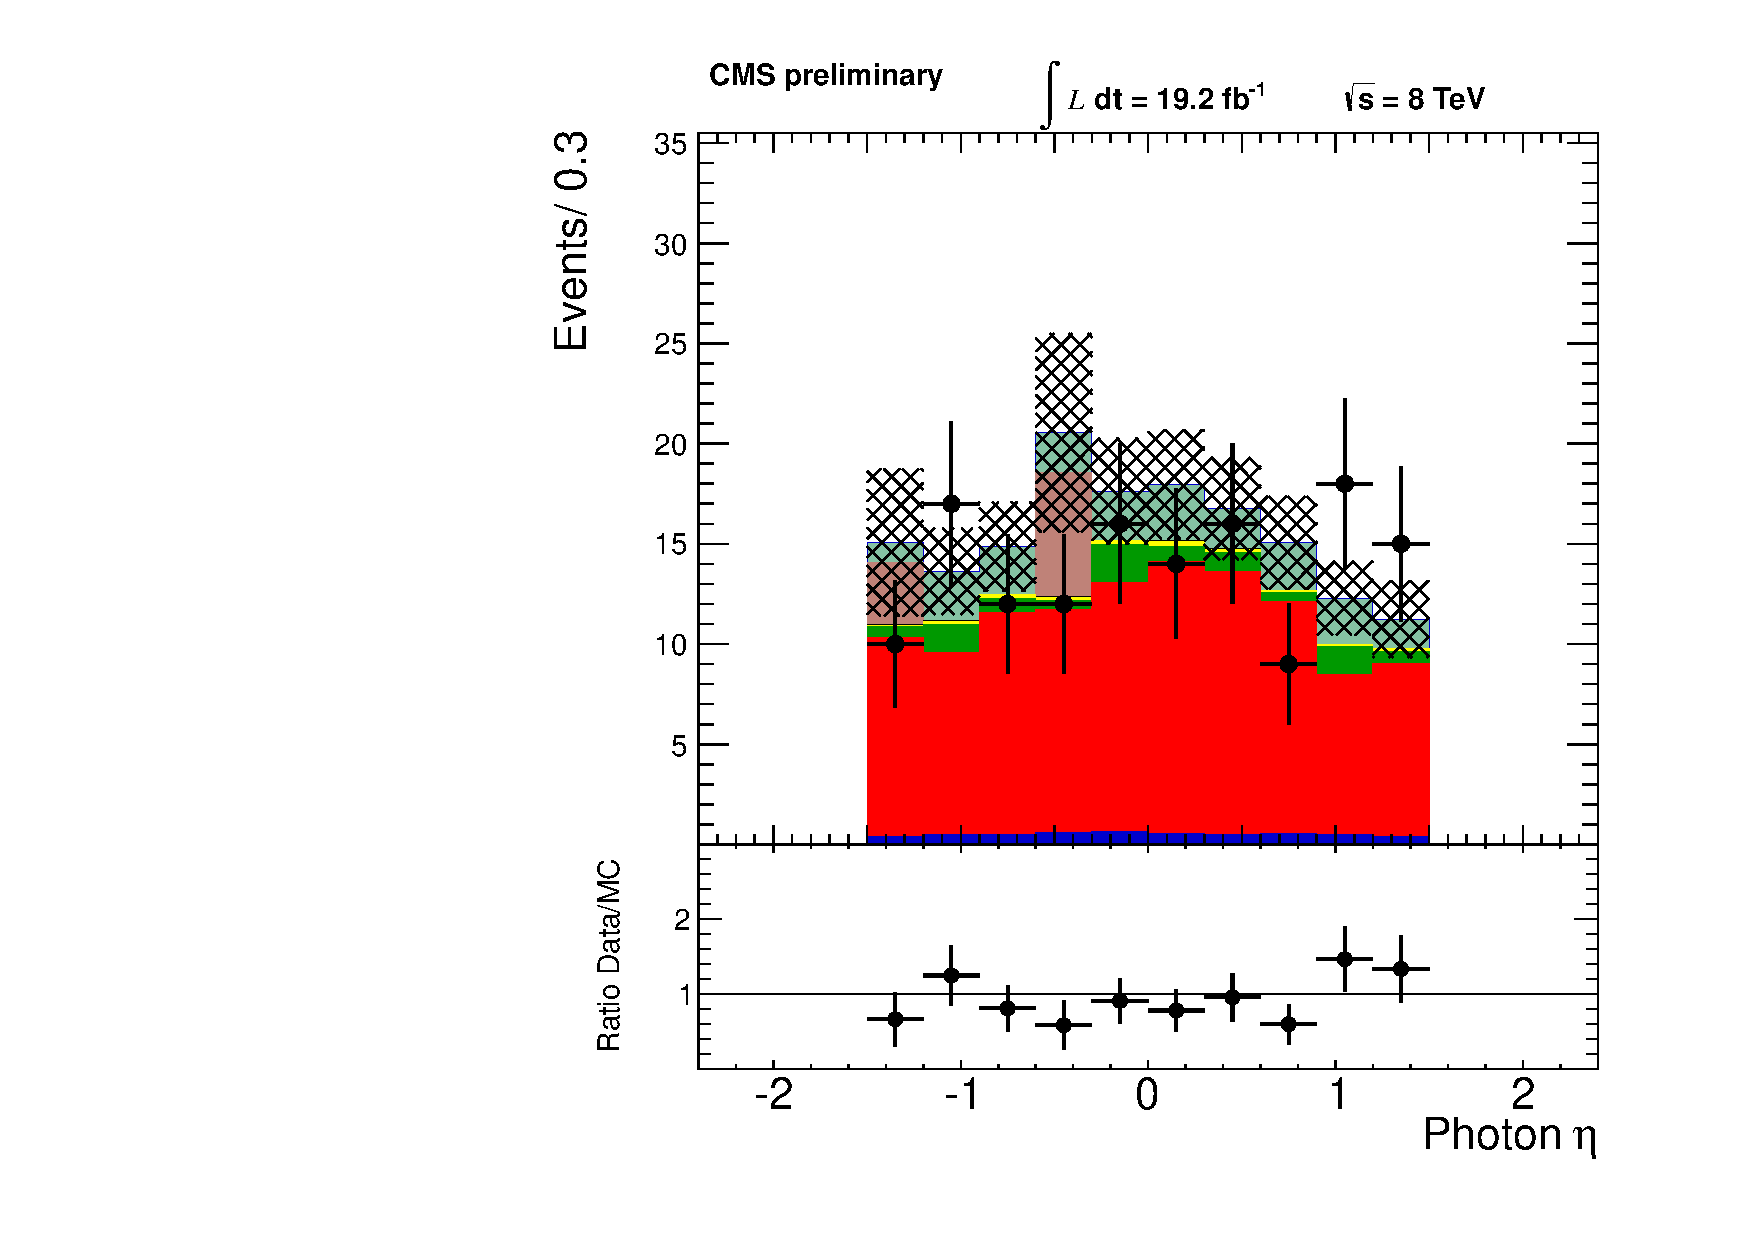
\includegraphics[width=.32\textwidth]{figs/el_Photon_eta.pdf}
}
\subfigure[]{
   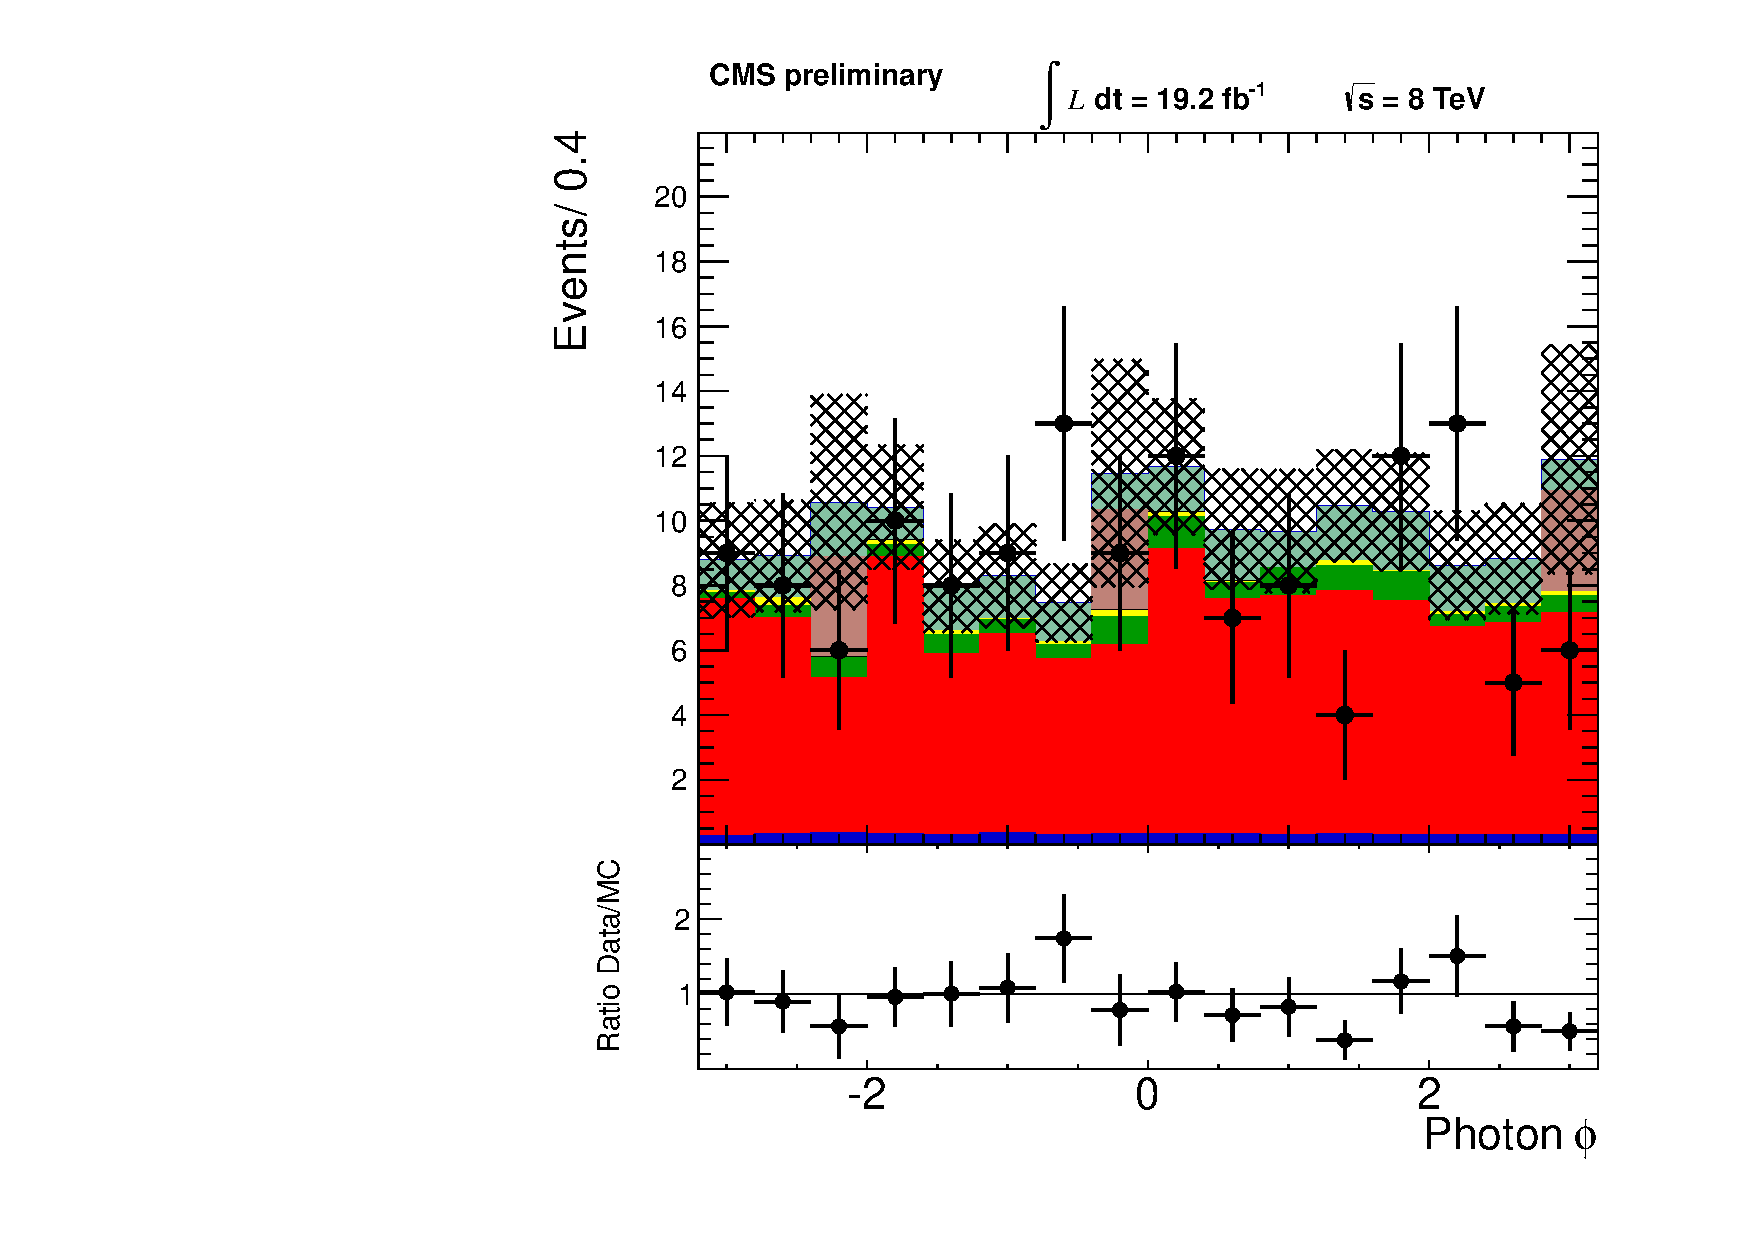
\includegraphics[width=.32\textwidth]{figs/el_Photon_phi.pdf}
}
\caption{Data and MC comparison plots for muon channel photon $p_{T}$ (a), $\eta$ (b), $\phi$ (c), and electron channel photon $p_{T}$ (d), $\eta$ (e), $\phi$ (f)}
\label{photonplots}
\end{center}
\end{figure}

\begin{figure}[b]
\begin{center}
\subfigure[]{
   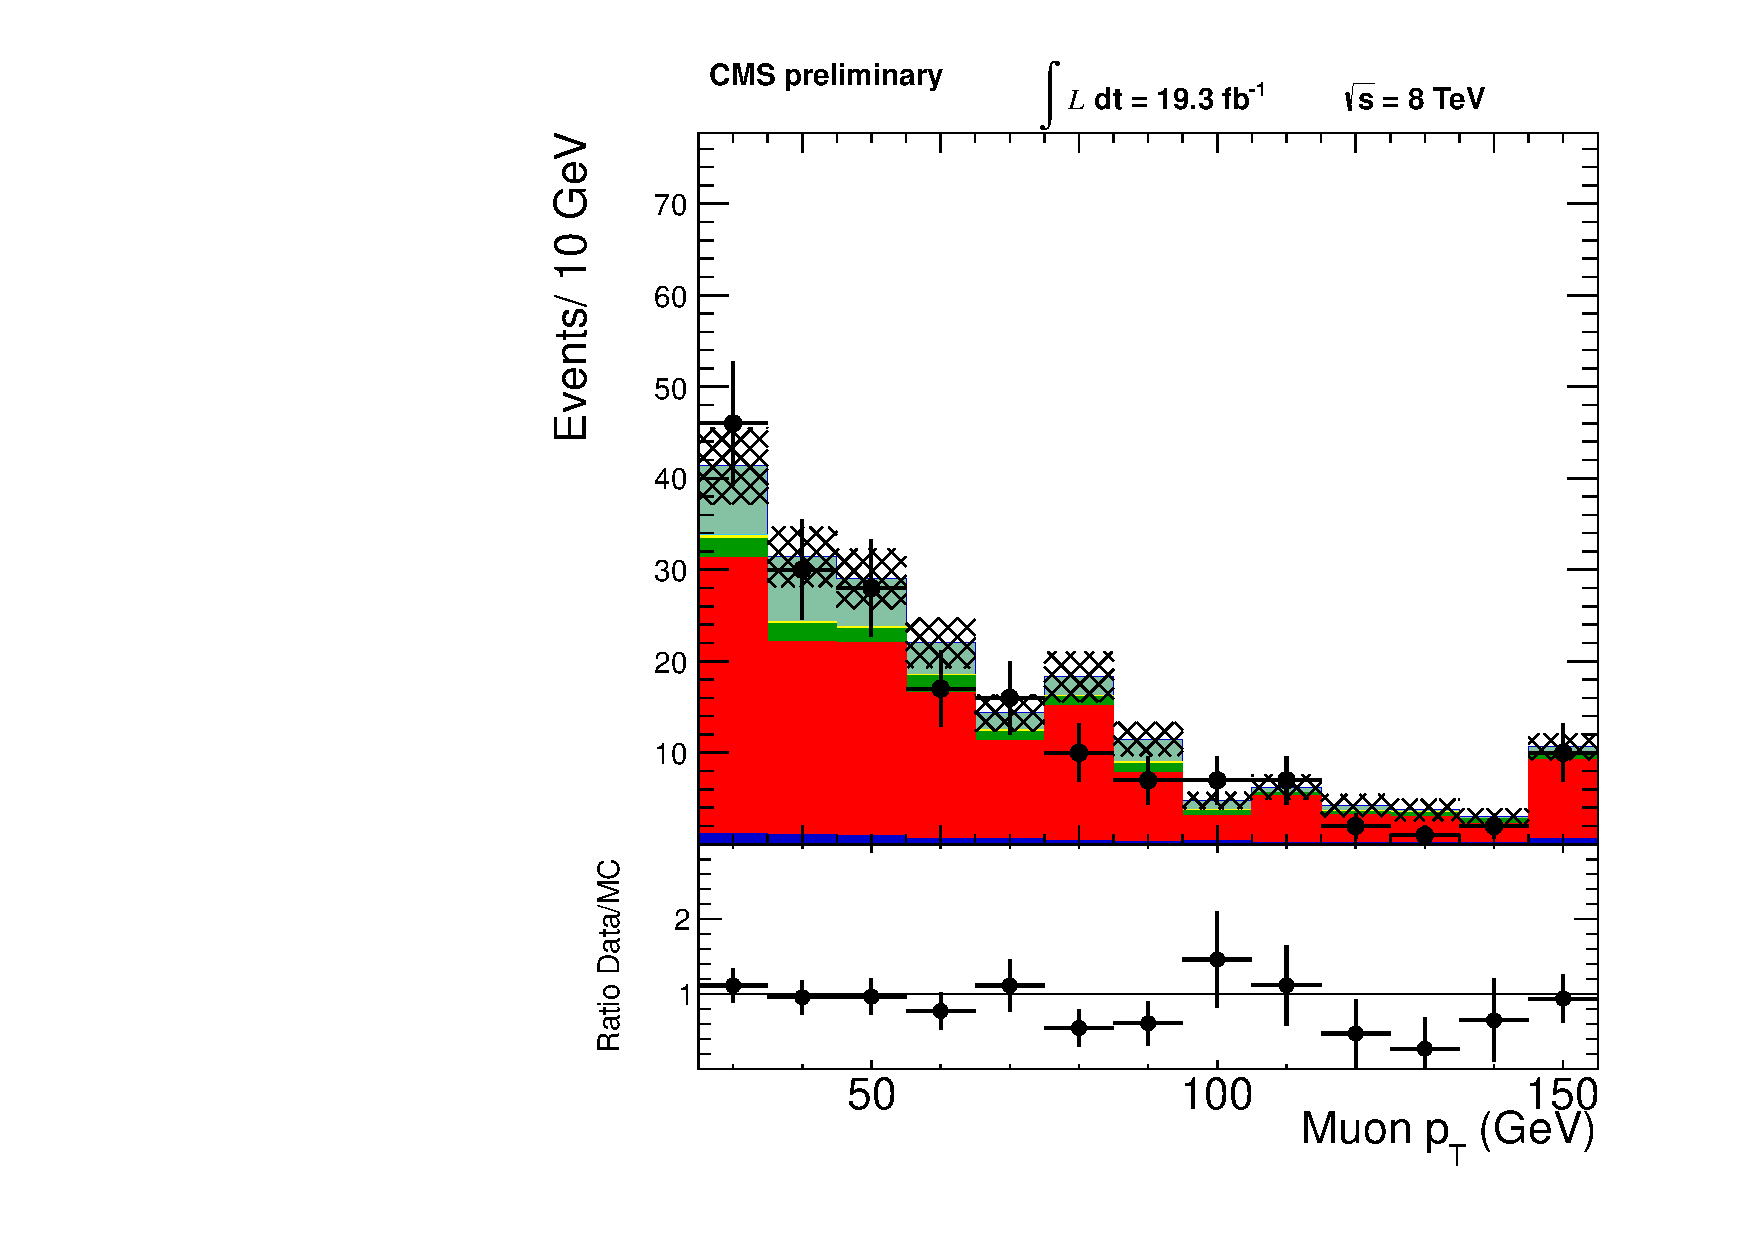
\includegraphics[width=.32\textwidth]{figs/mu_W_muon_pt.pdf}
}   
\subfigure[]{
   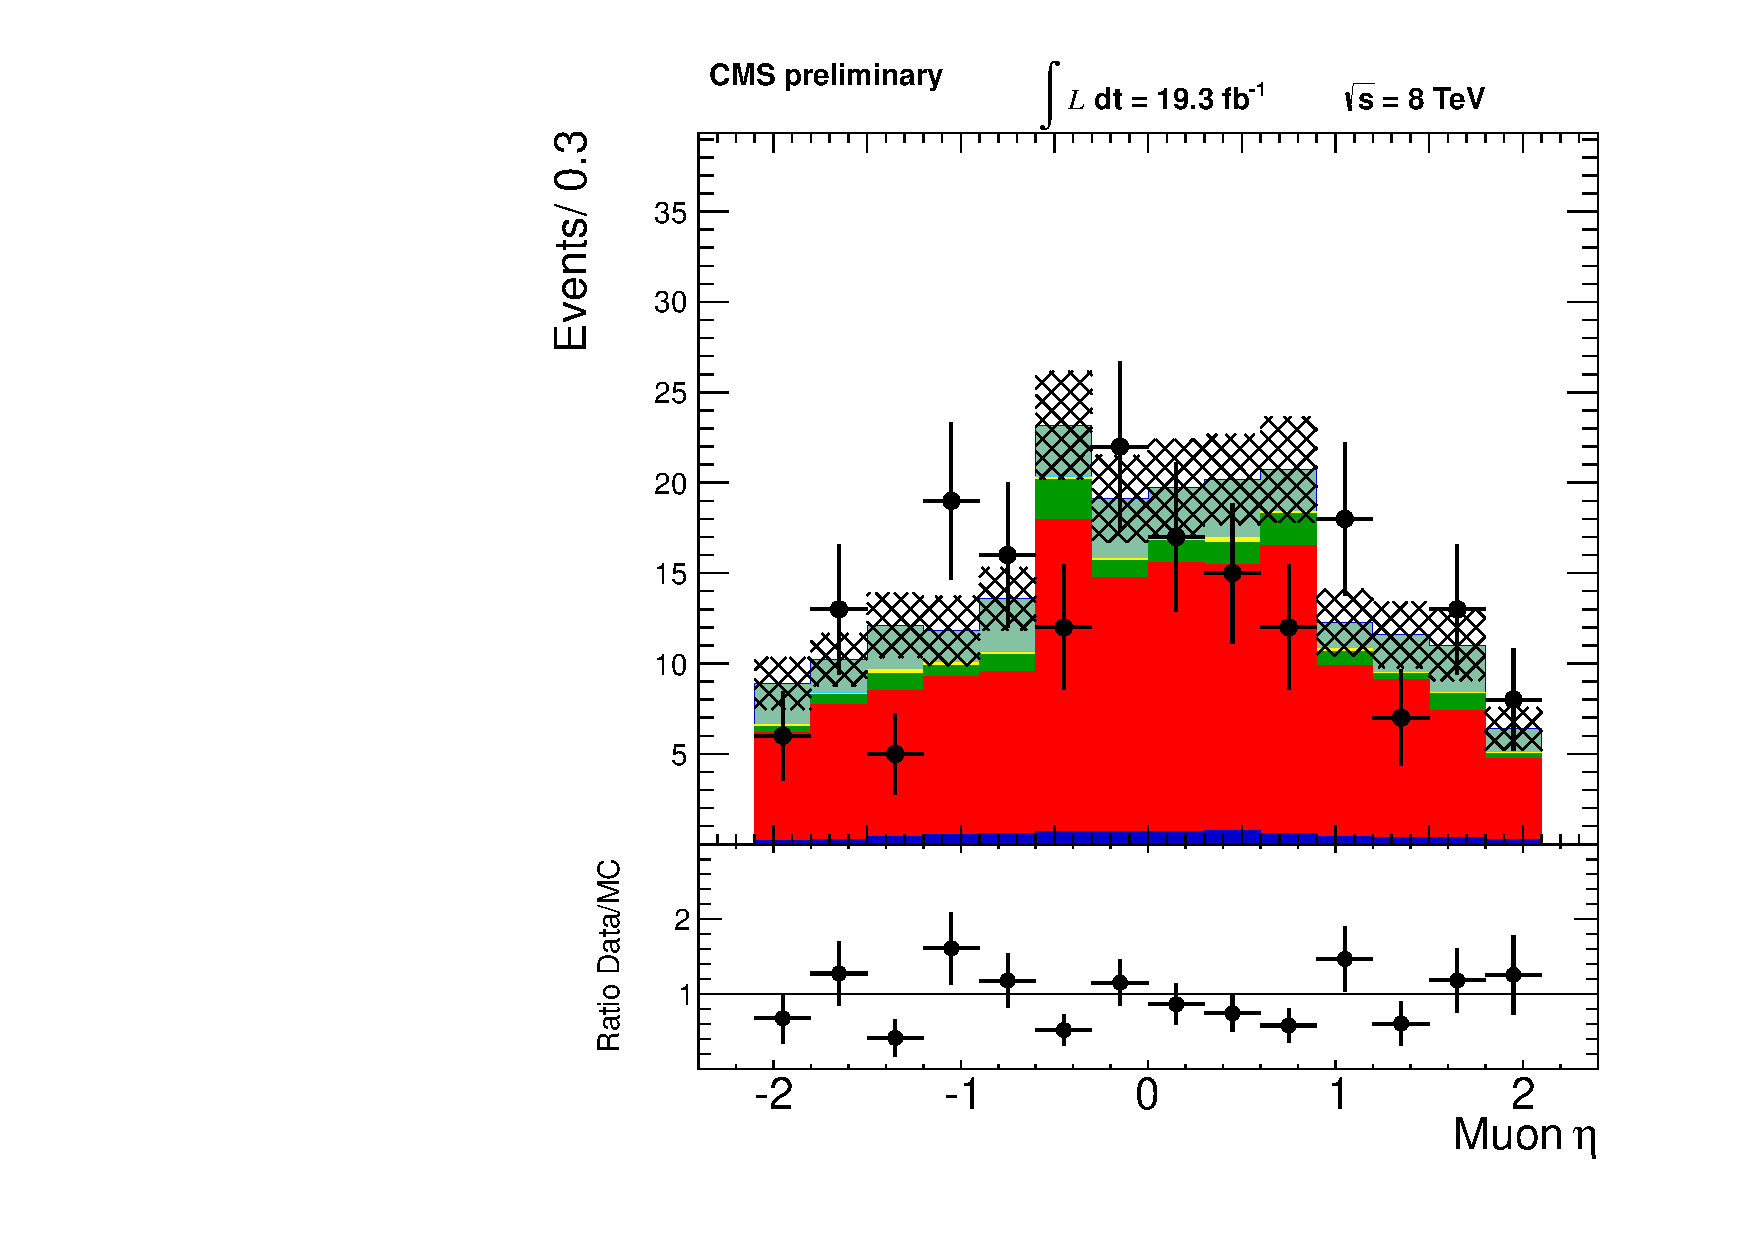
\includegraphics[width=.32\textwidth]{figs/mu_W_muon_eta.pdf}
}   
\subfigure[]{
   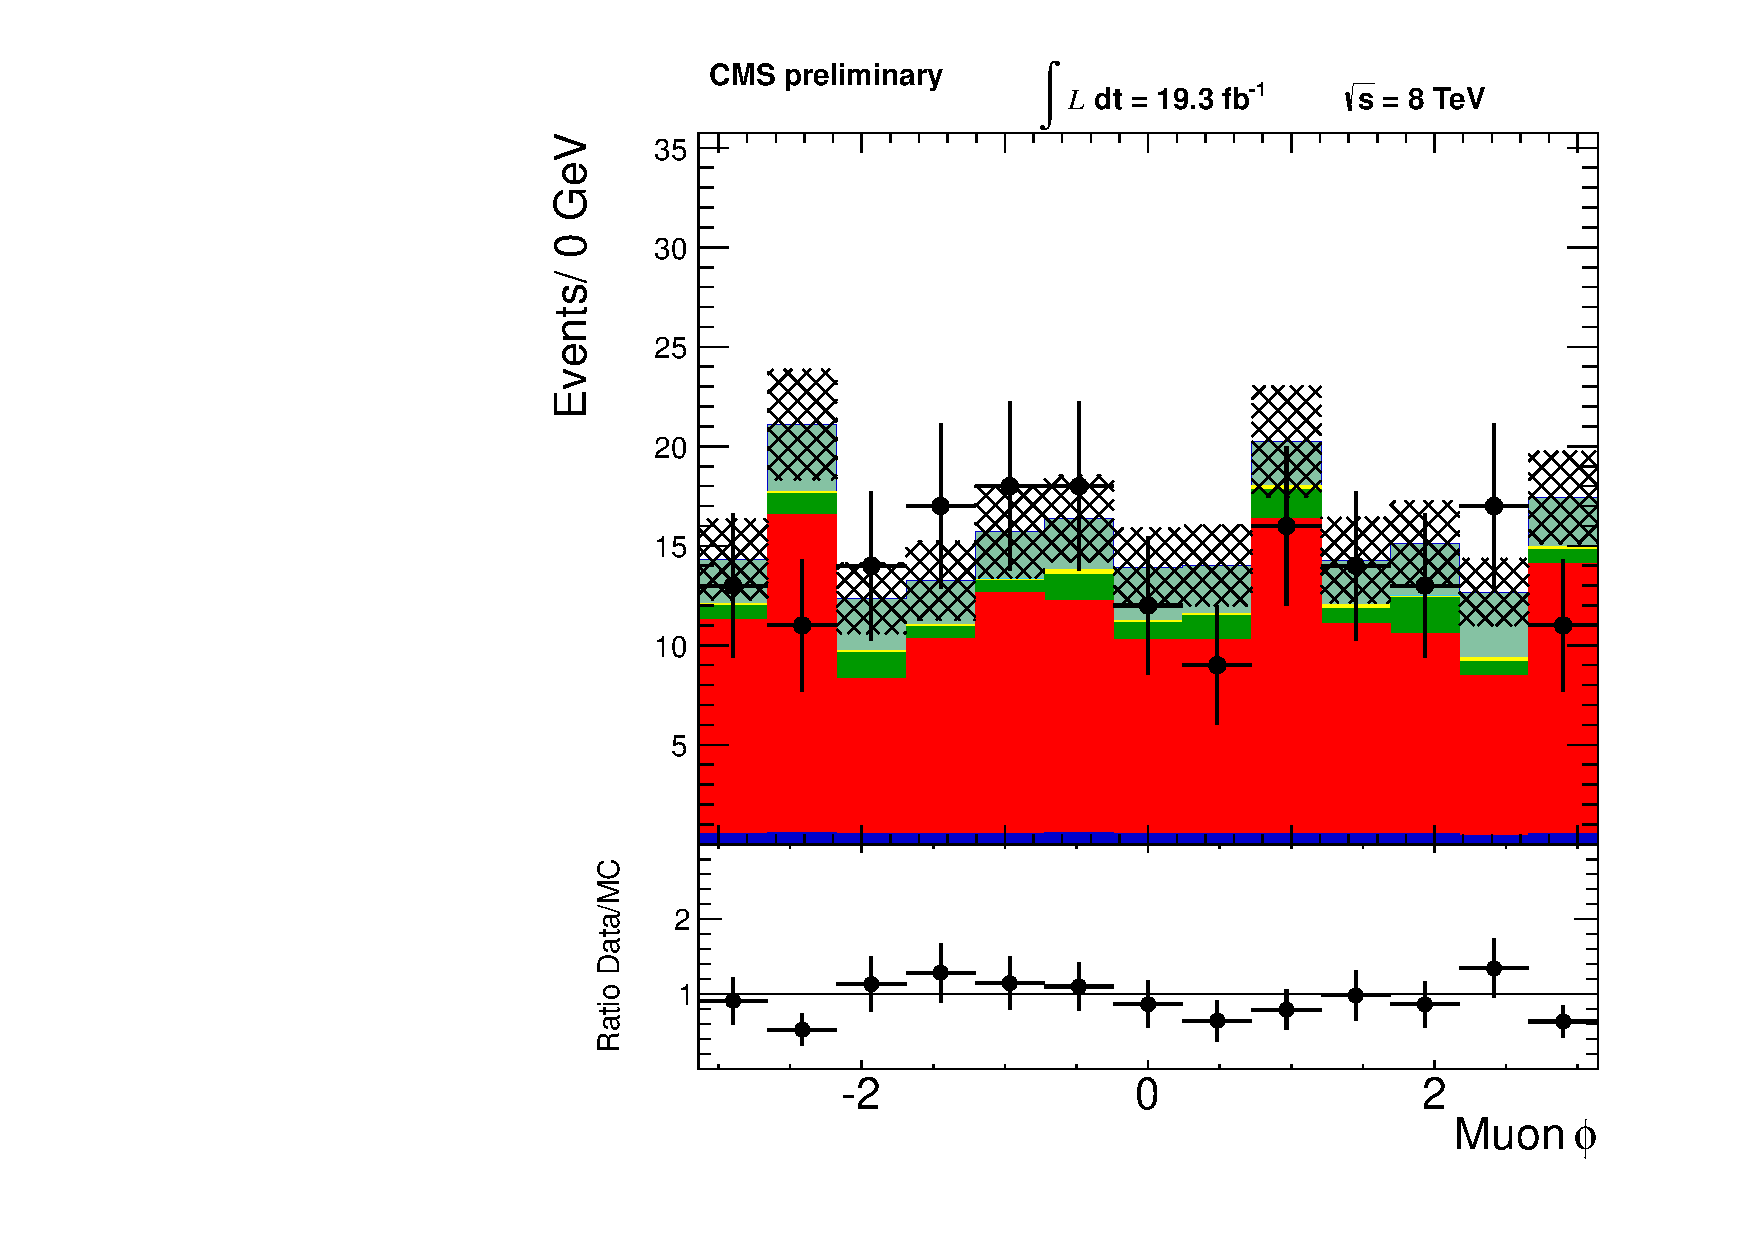
\includegraphics[width=.32\textwidth]{figs/mu_W_muon_phi.pdf}
}
\caption{Data and MC comparison plots for muon $p_{T}$ (a), $\eta$ (b), $\phi$ (c)}
\label{muonplots}
\end{center}
\end{figure}

\begin{figure}[b]
\begin{center}
\subfigure[]{
   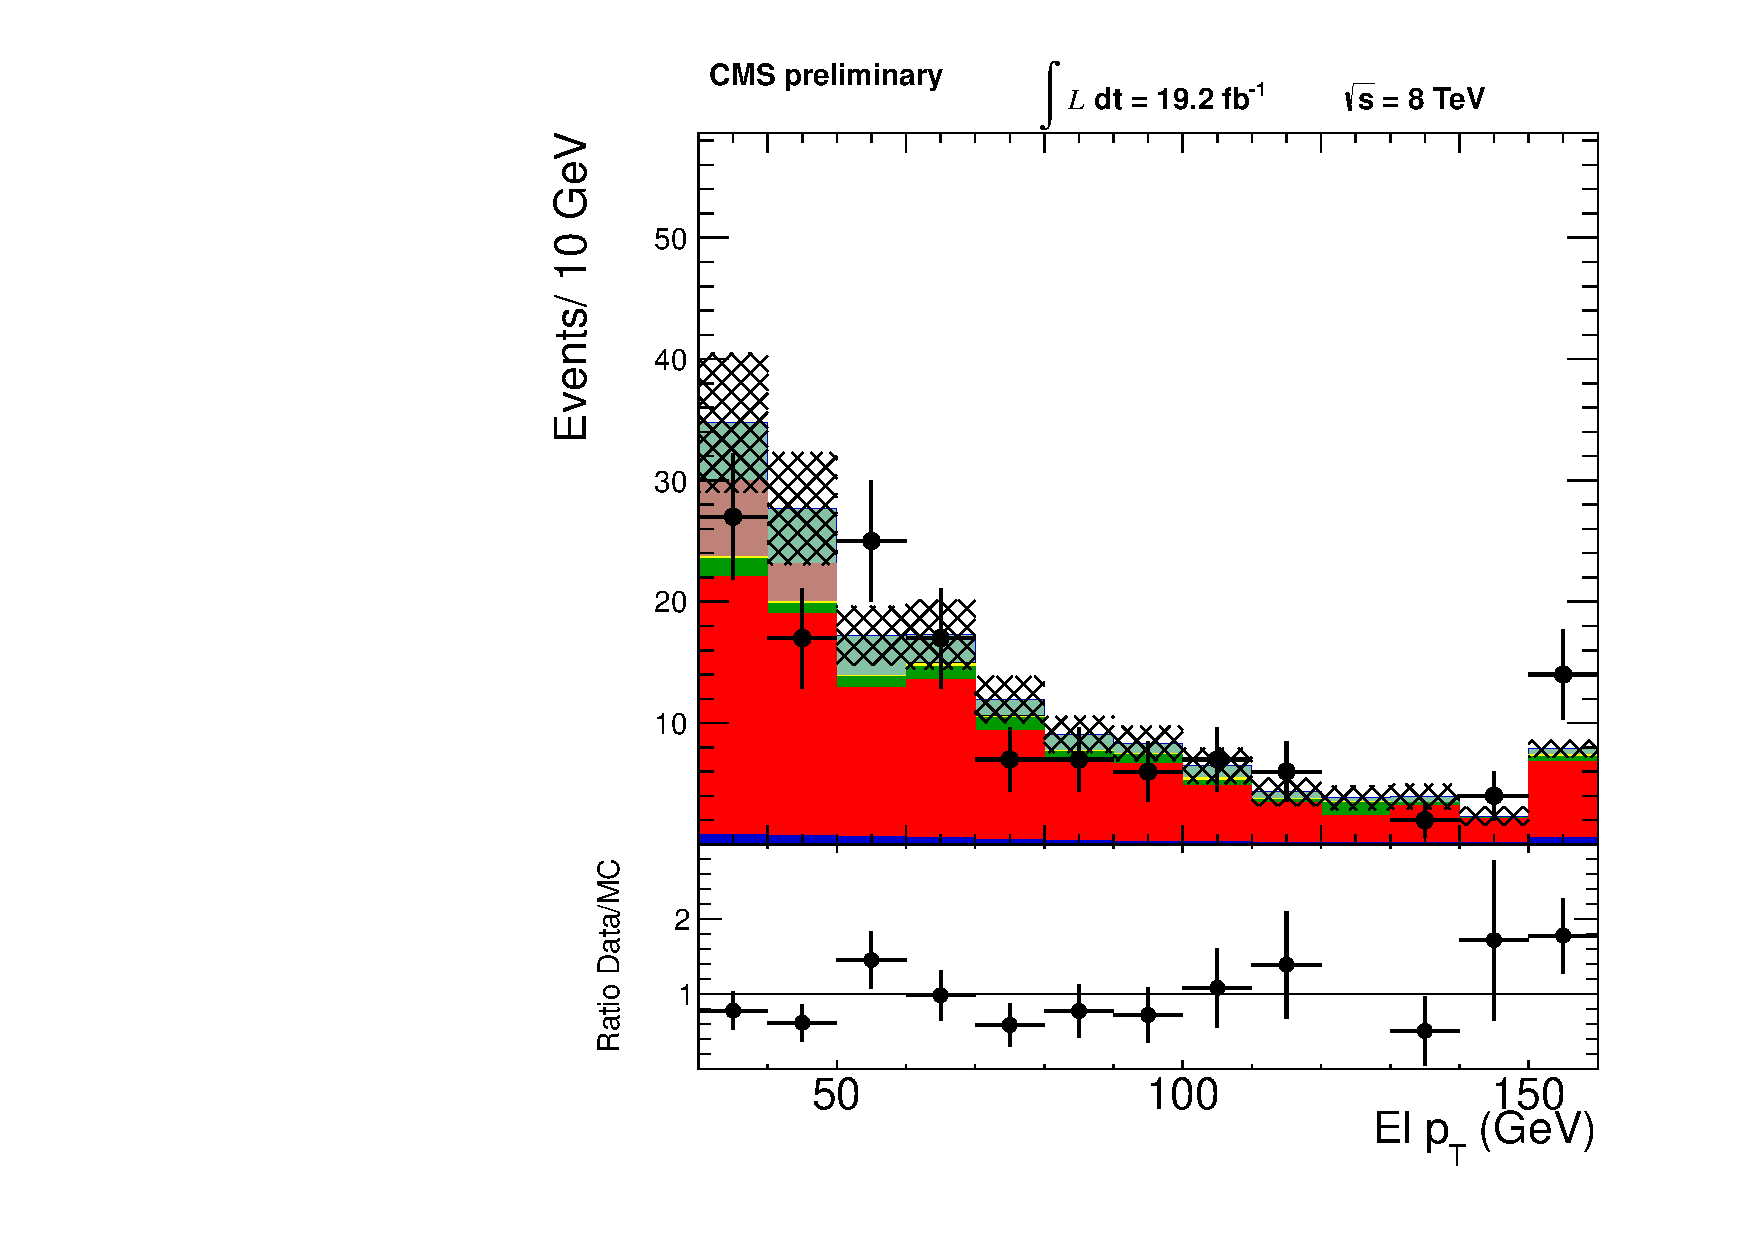
\includegraphics[width=.32\textwidth]{figs/el_W_electron_pt.pdf}
}   
\subfigure[]{
   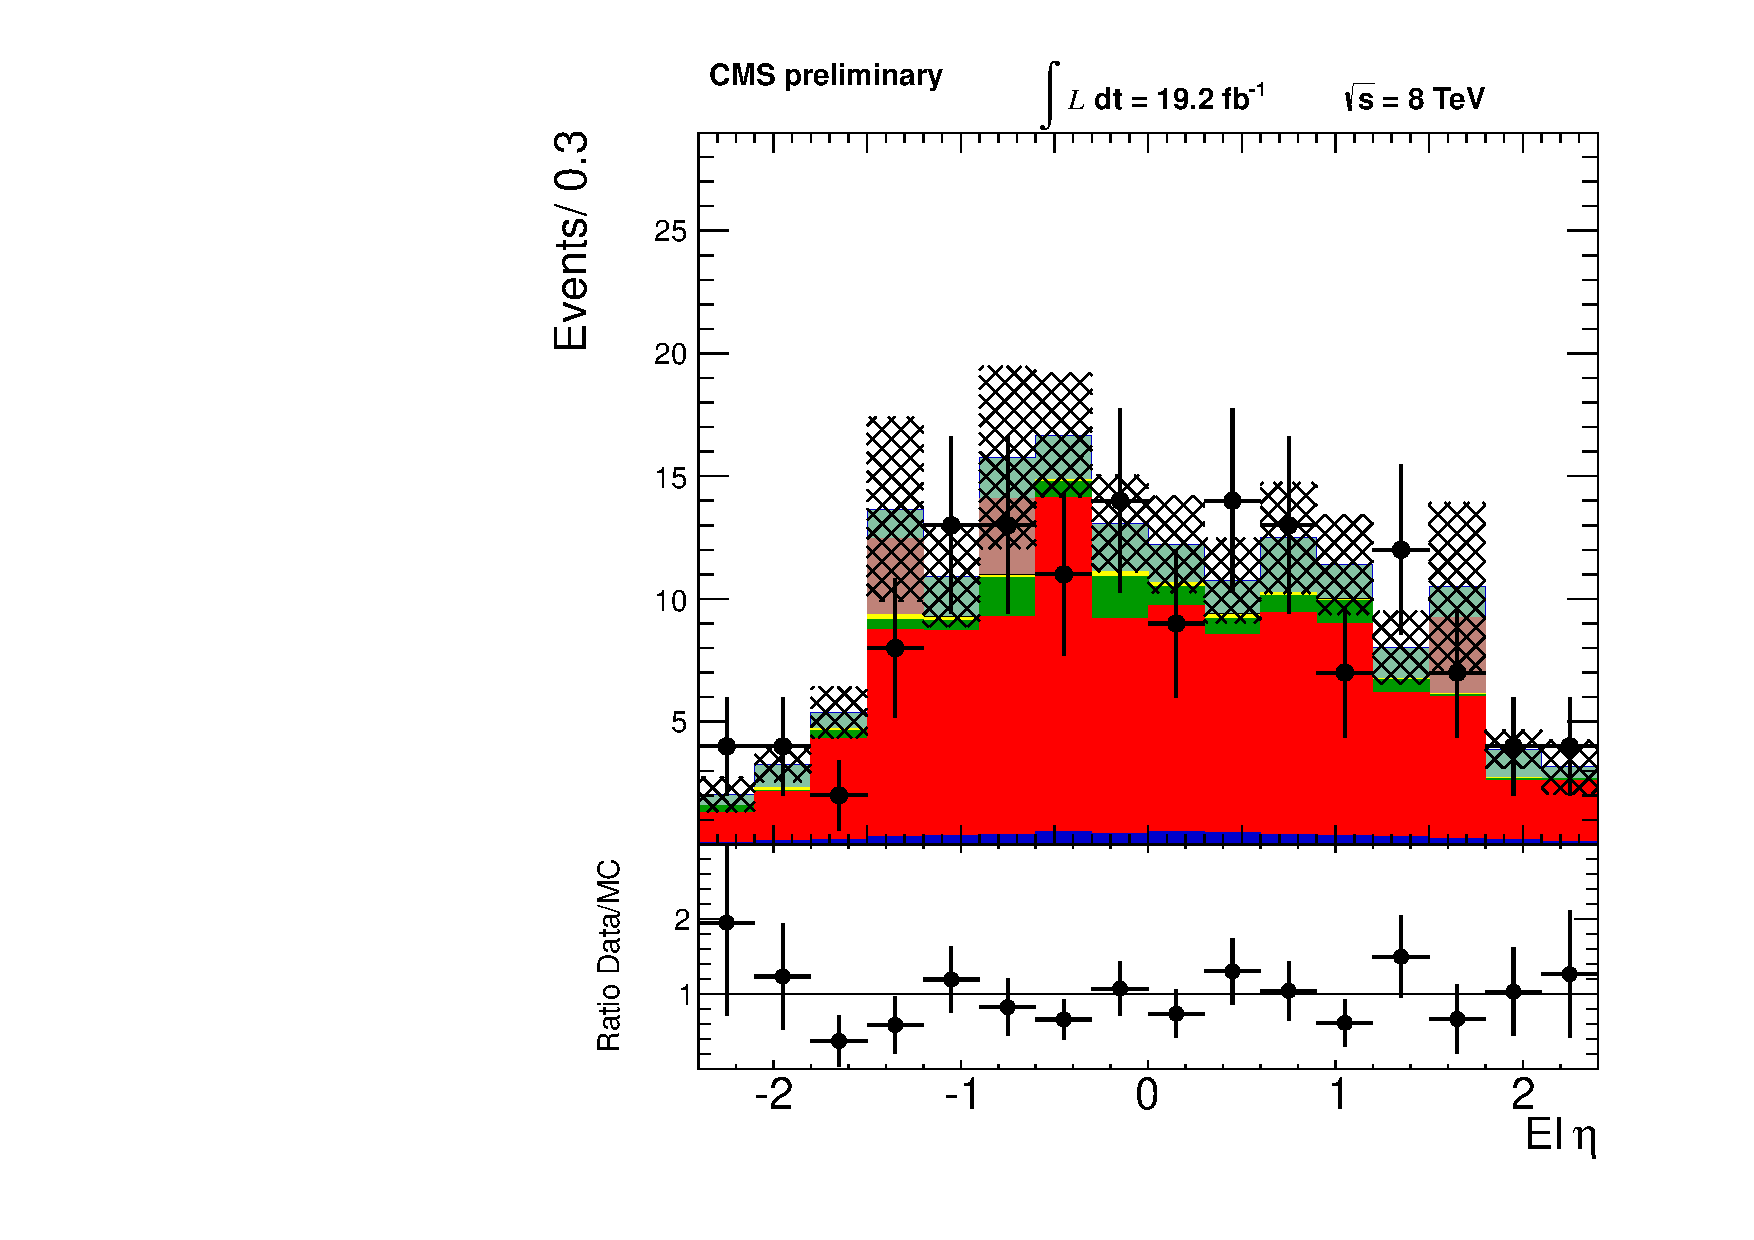
\includegraphics[width=.32\textwidth]{figs/el_W_electron_eta.pdf}
}   
\subfigure[]{
   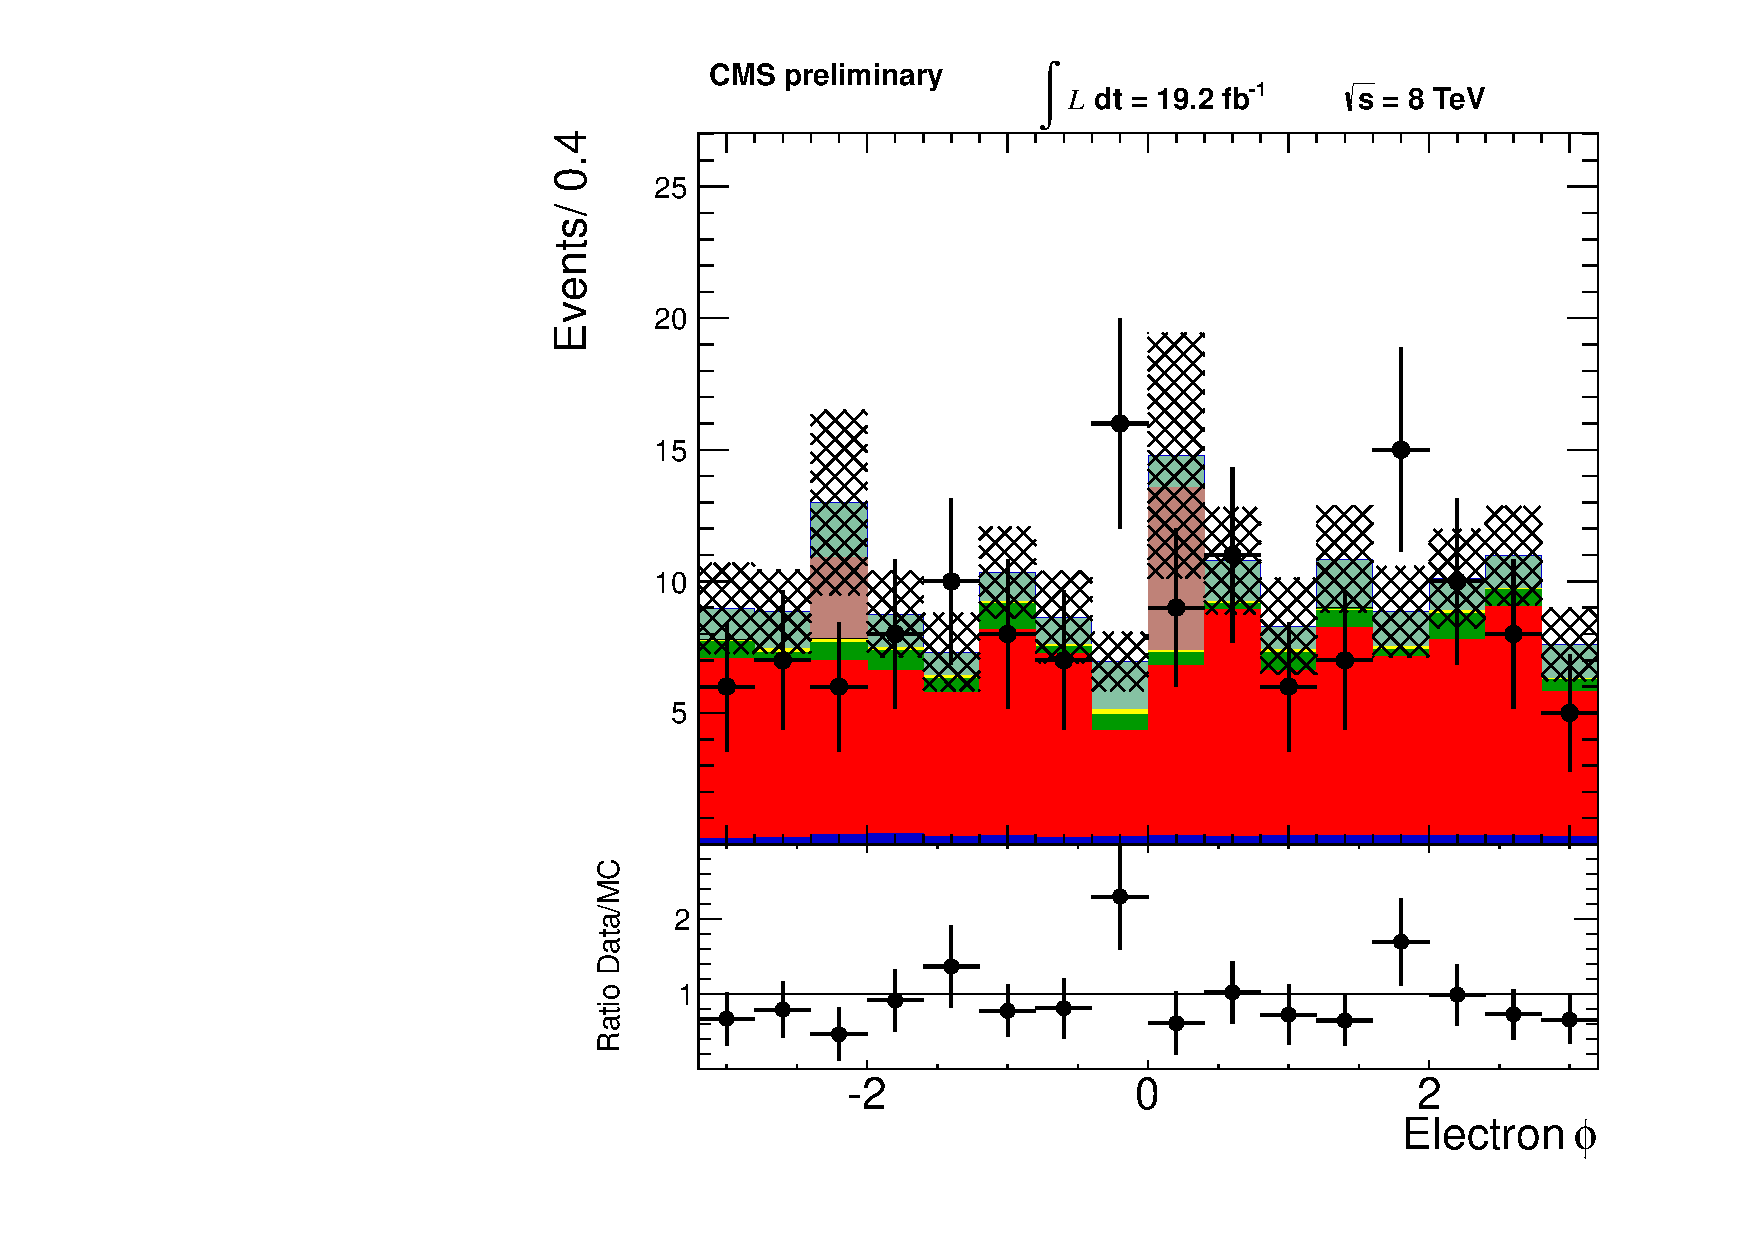
\includegraphics[width=.32\textwidth]{figs/el_W_electron_phi.pdf}
}
\caption{Data and MC comparison plots for electron $p_{T}$ (a), $\eta$ (b), $\phi$ (c)}
\label{elecplots}
\end{center}
\end{figure}

\begin{figure}[b]
\begin{center}
\subfigure[]{
   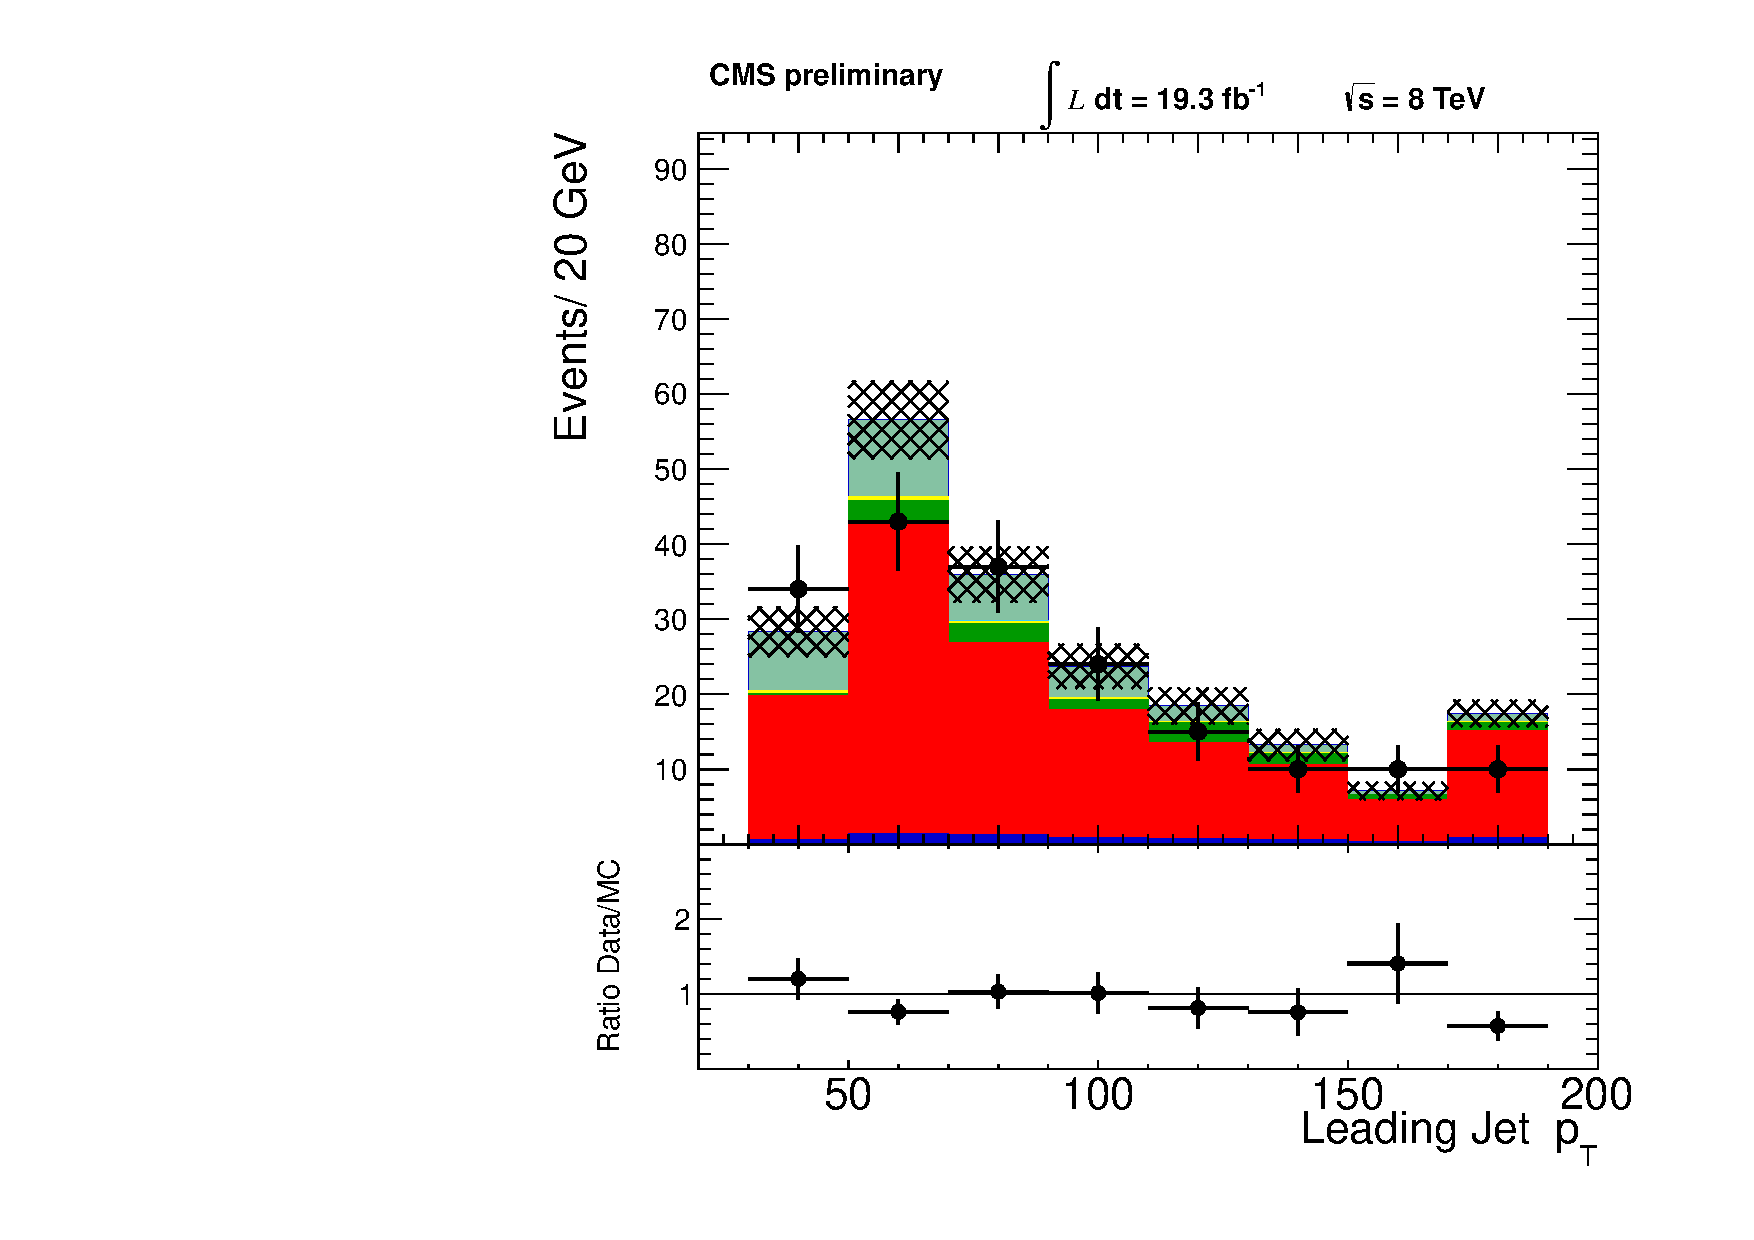
\includegraphics[width=.32\textwidth]{figs/mu_jetld_pt.pdf}
}   
\subfigure[]{
   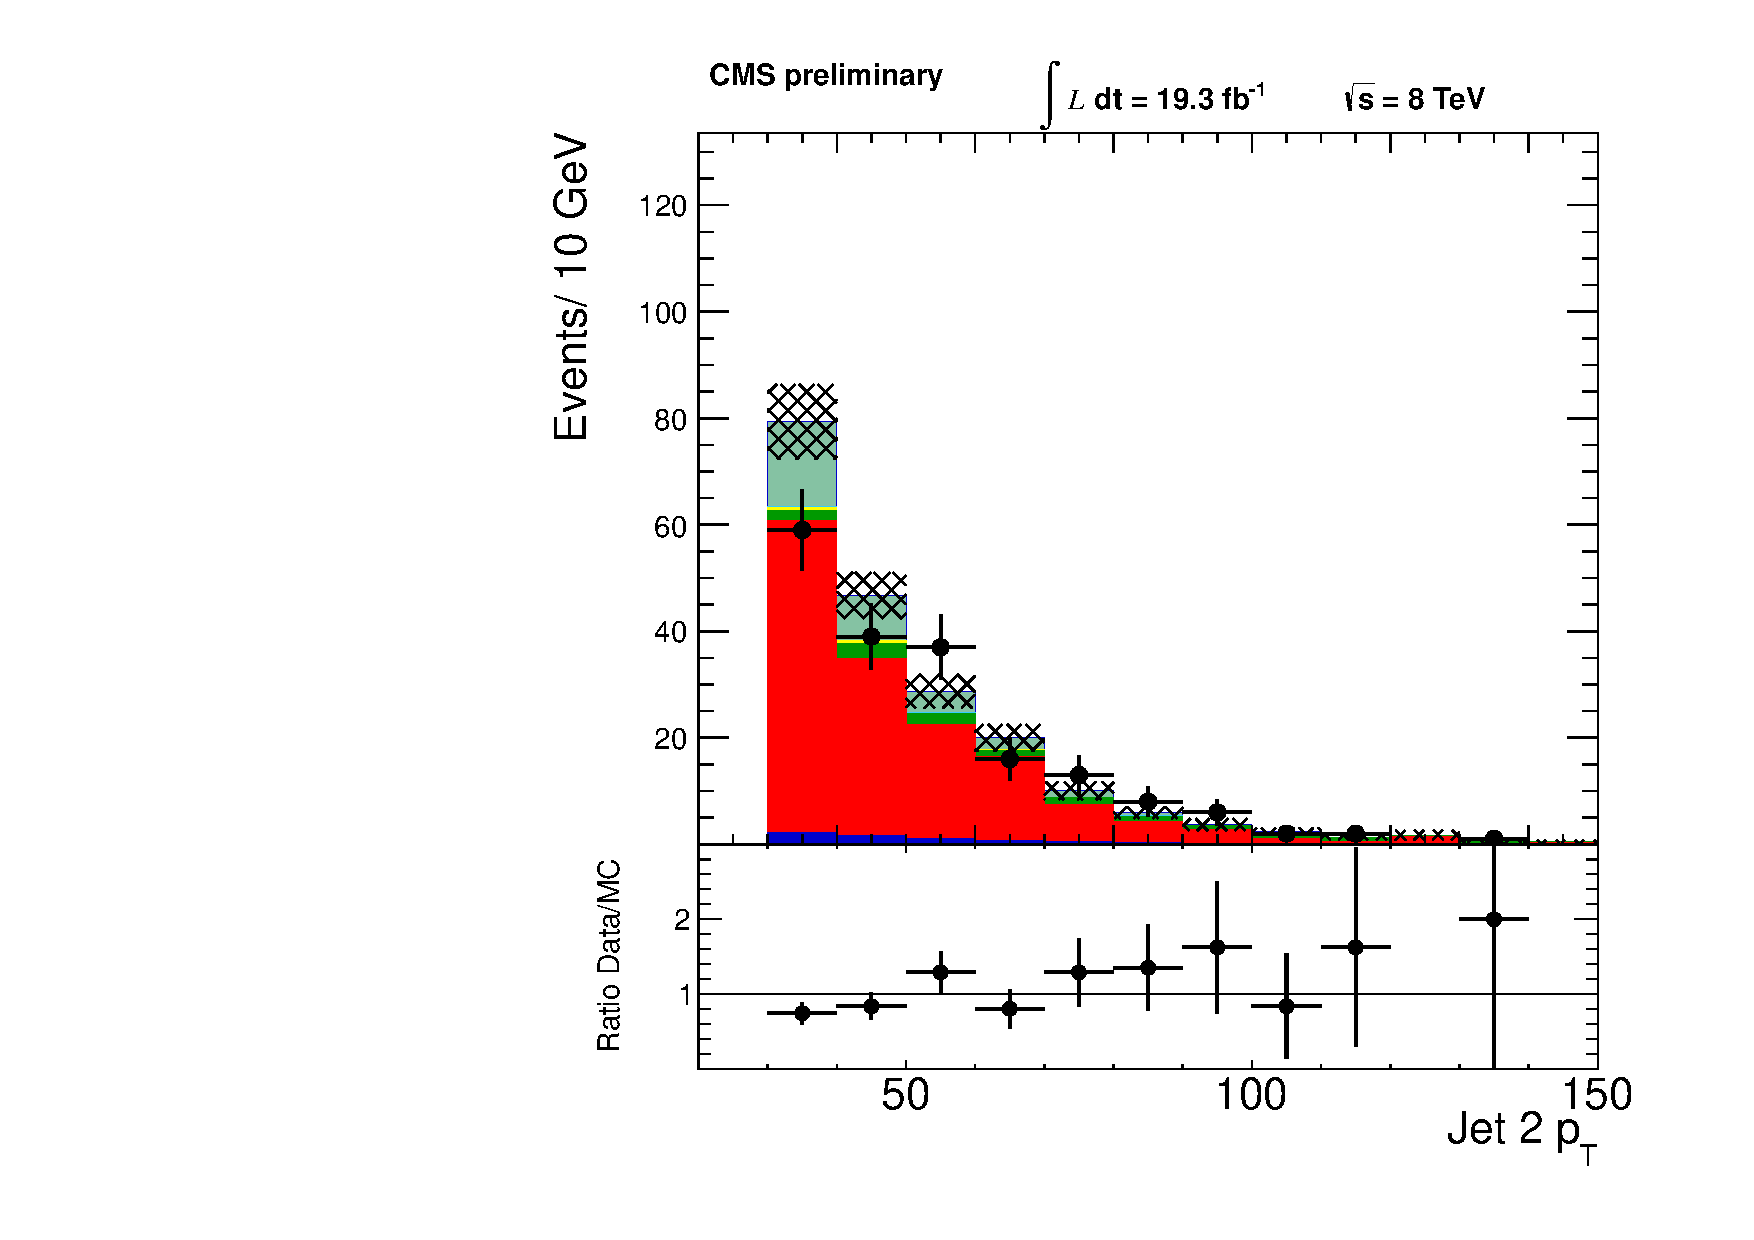
\includegraphics[width=.32\textwidth]{figs/mu_jetnt_pt.pdf}
}   
\subfigure[]{
   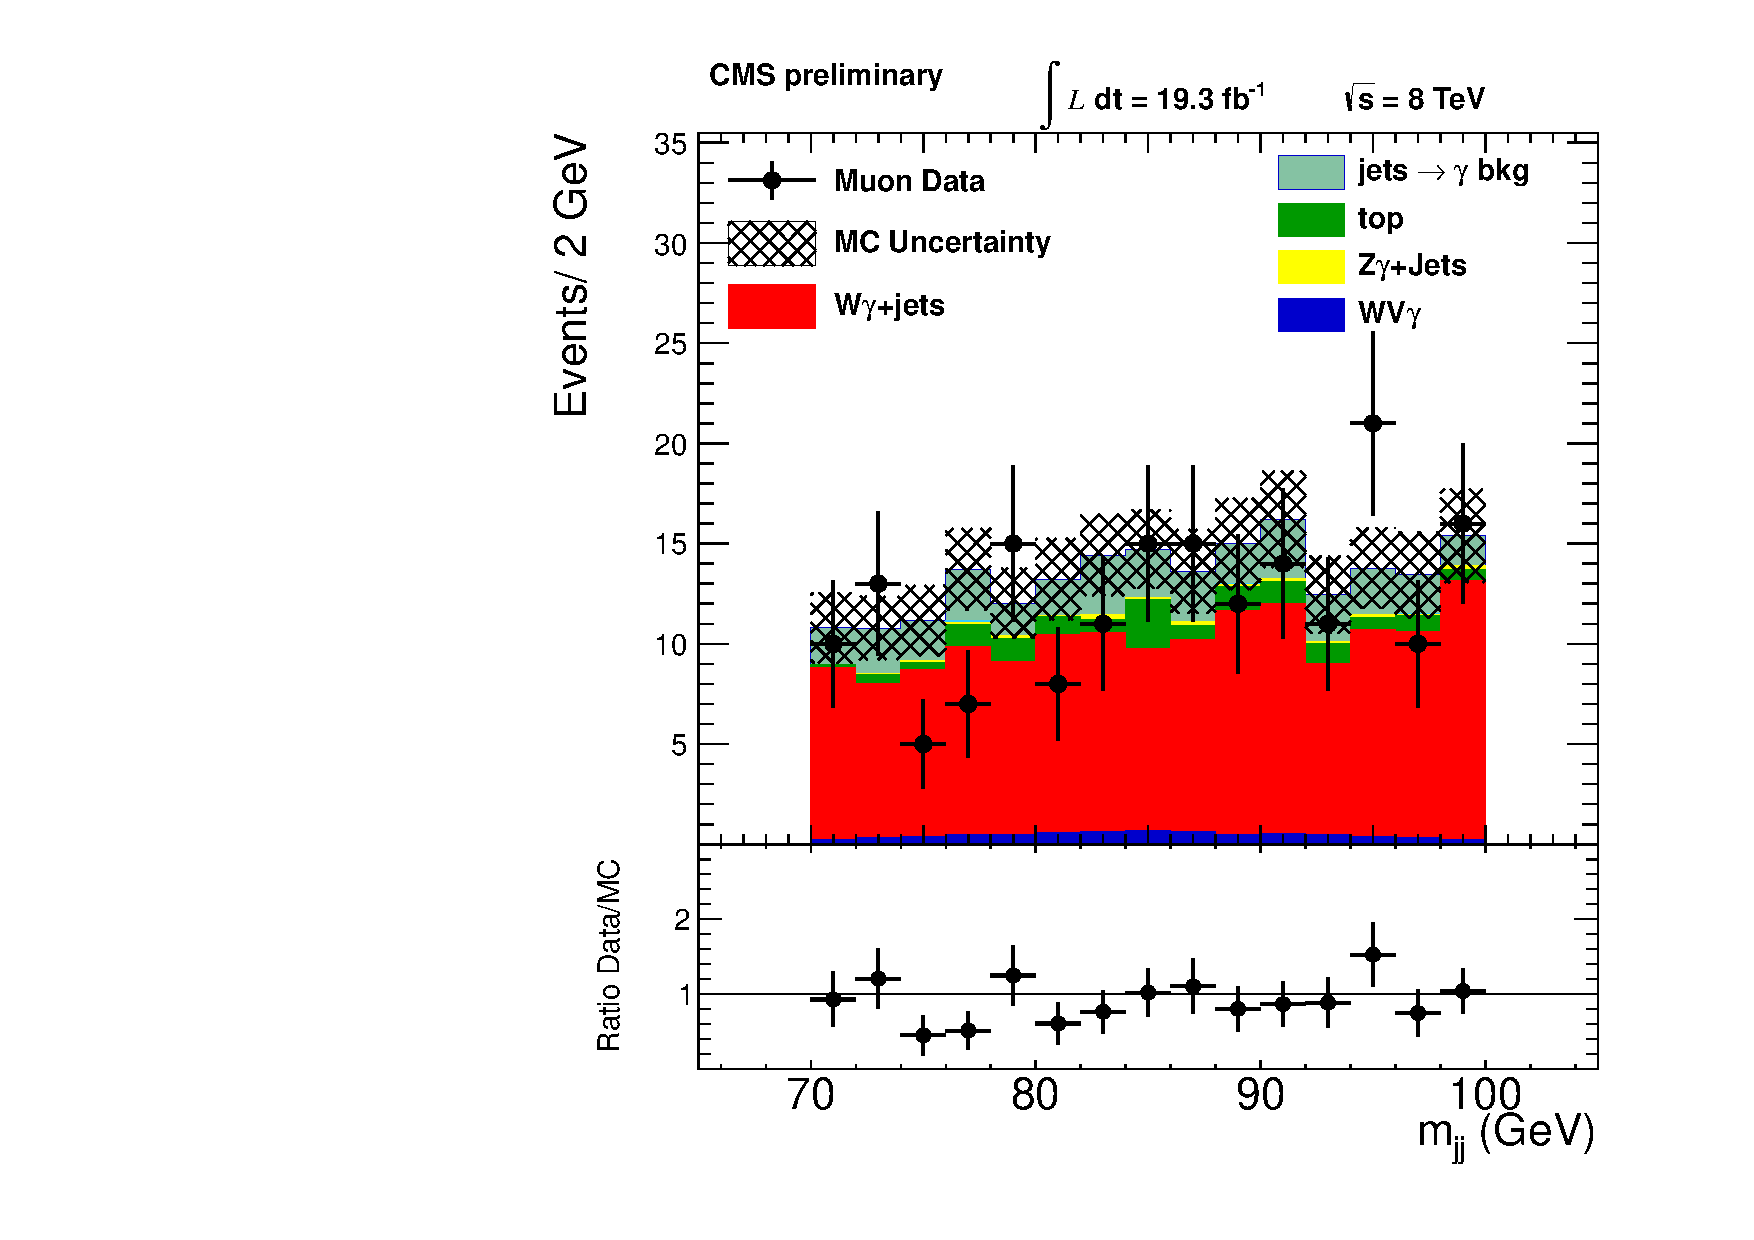
\includegraphics[width=.32\textwidth]{figs/mu_mjj.pdf}
}   \\
\subfigure[]{
   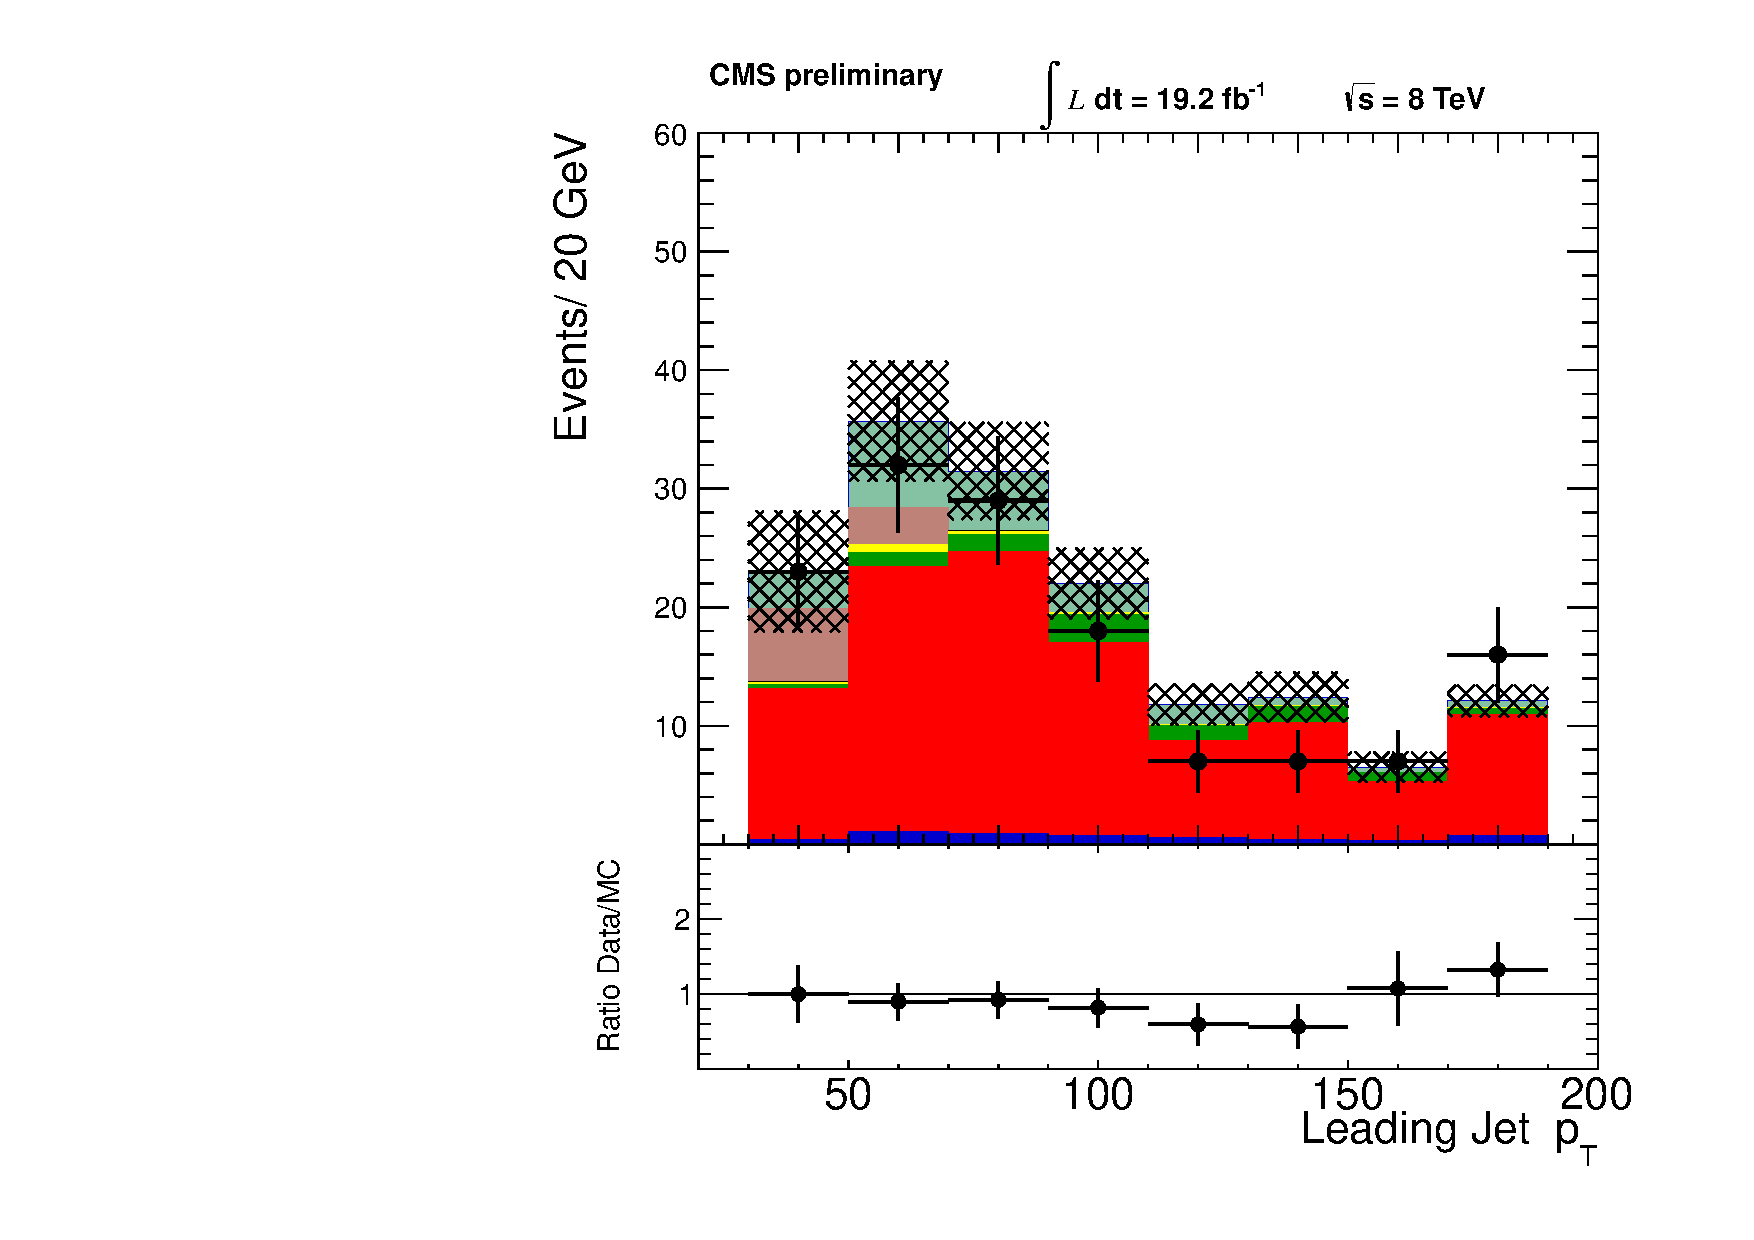
\includegraphics[width=.32\textwidth]{figs/el_jetld_pt.pdf}
}   
\subfigure[]{
   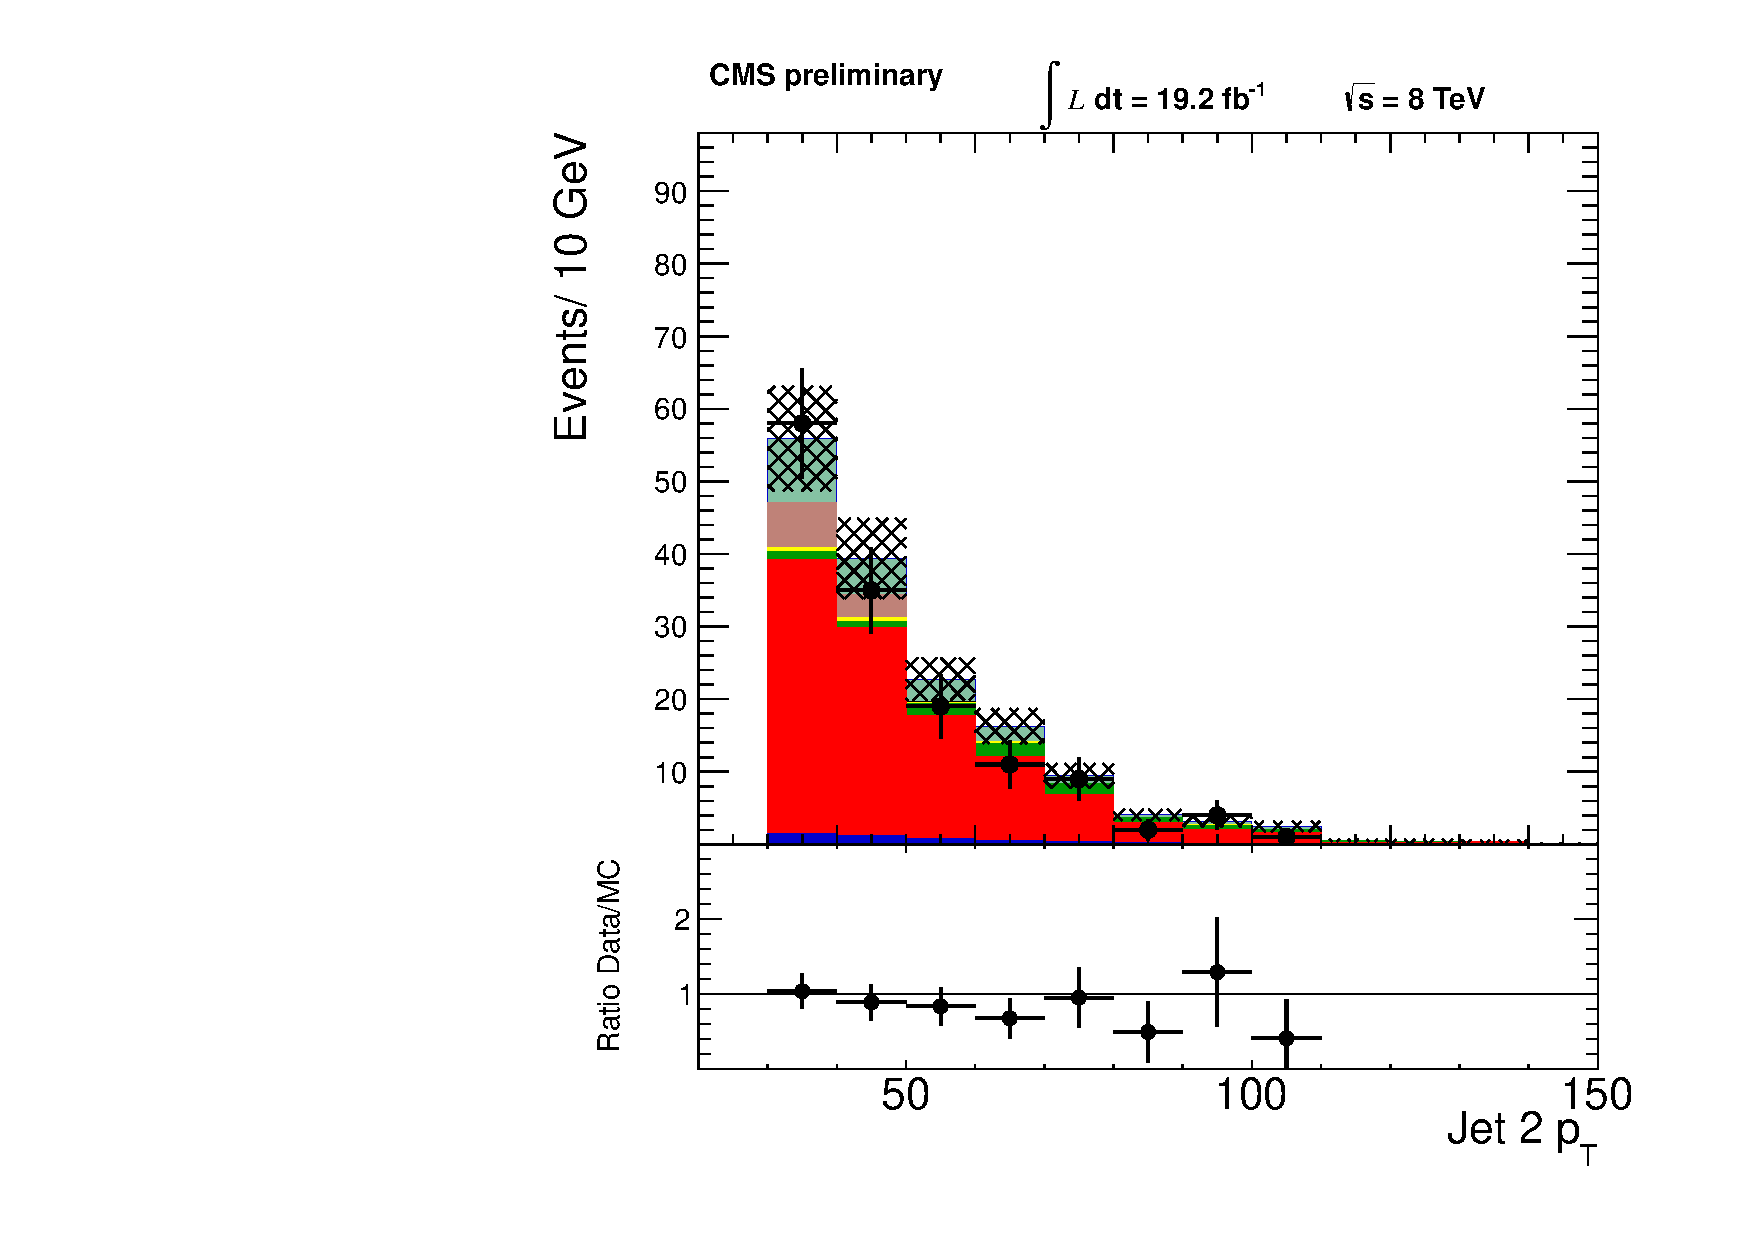
\includegraphics[width=.32\textwidth]{figs/el_jetnt_pt.pdf}
}   
\subfigure[]{
   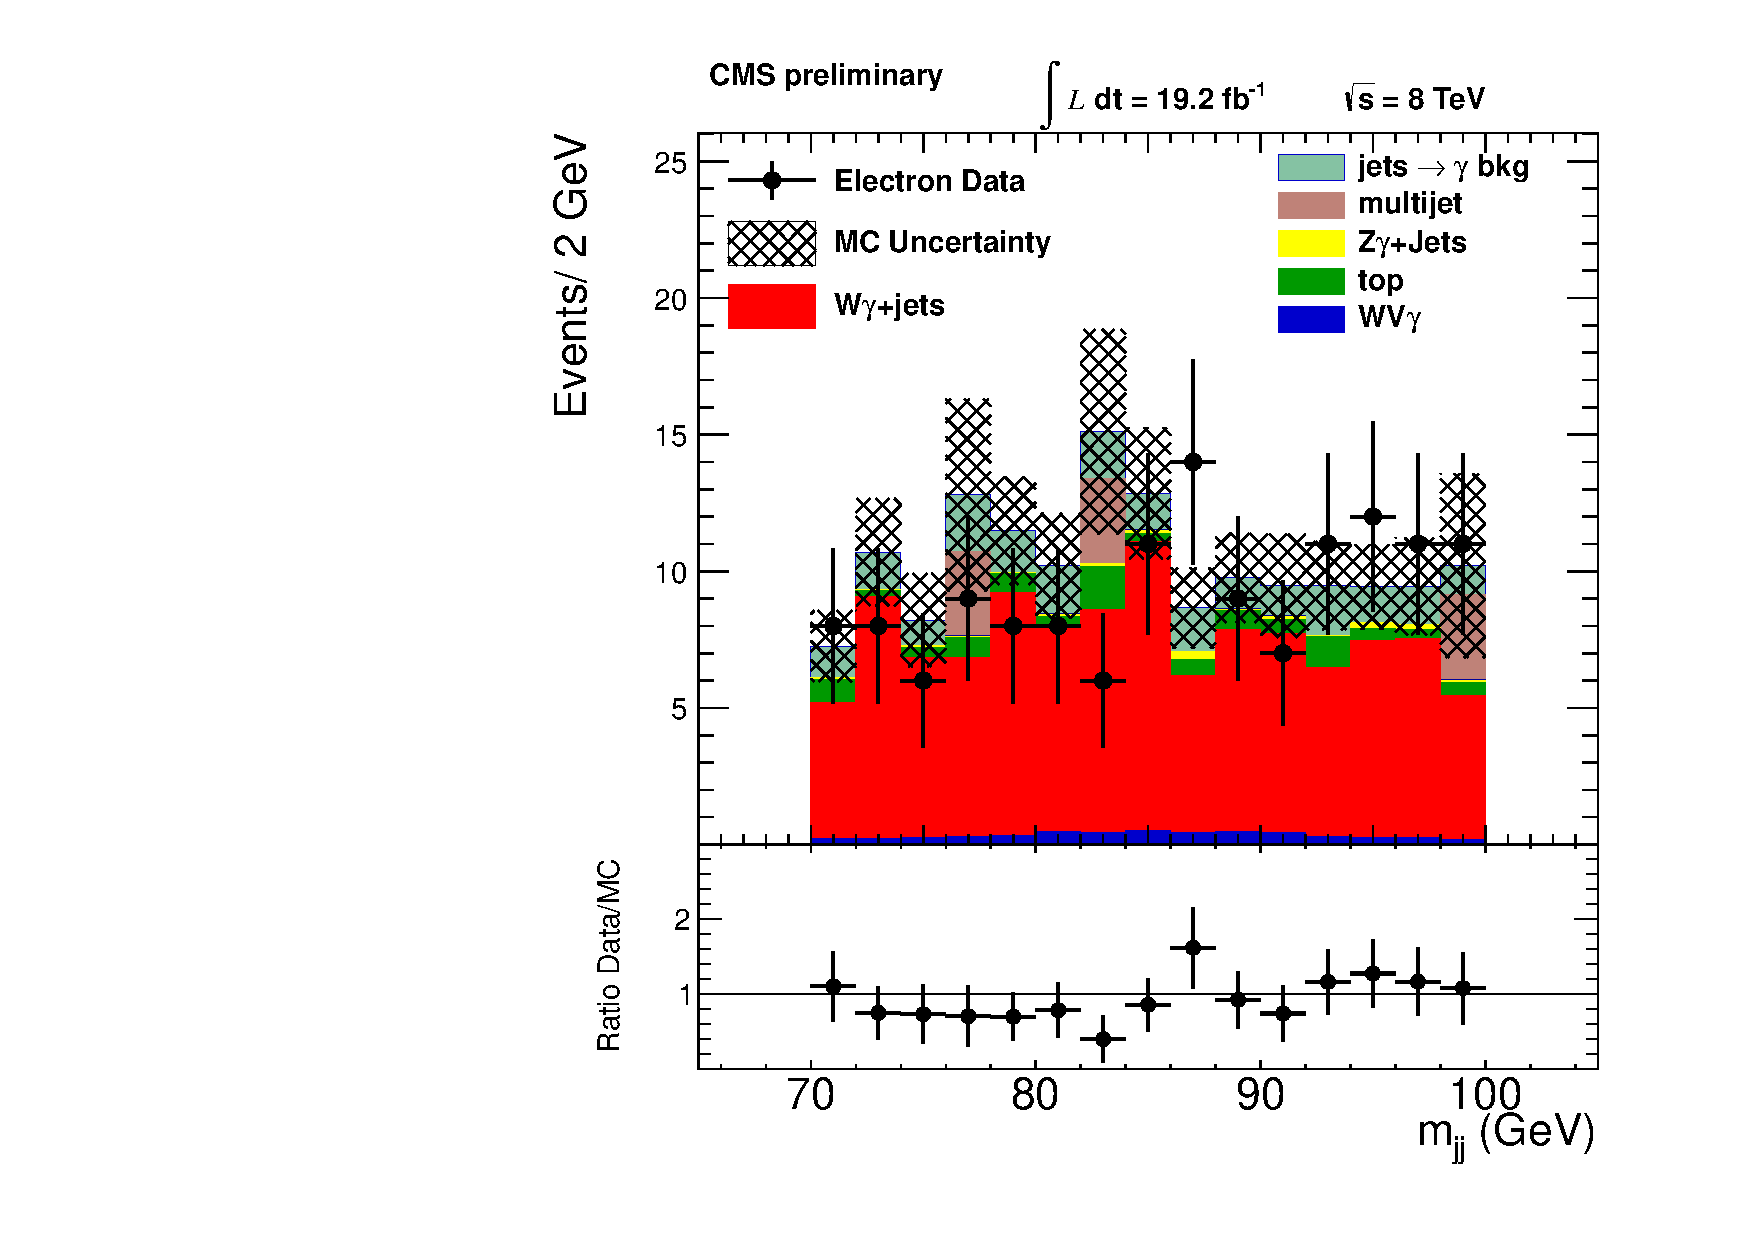
\includegraphics[width=.32\textwidth]{figs/el_mjj.pdf}
}   
\caption{Data and MC comparison plots for muon channel leading jet $p_{T}$ (a) second jet $p_{T}$ (b), di-jet mass (c);
muon channel leading jet $p_{T}$ (d) second jet $p_{T}$ (e) and di-jet mass (f)}
\label{mudijetplots}
\end{center}
\end{figure}

\begin{figure}[b]
\begin{center}
\subfigure[]{
   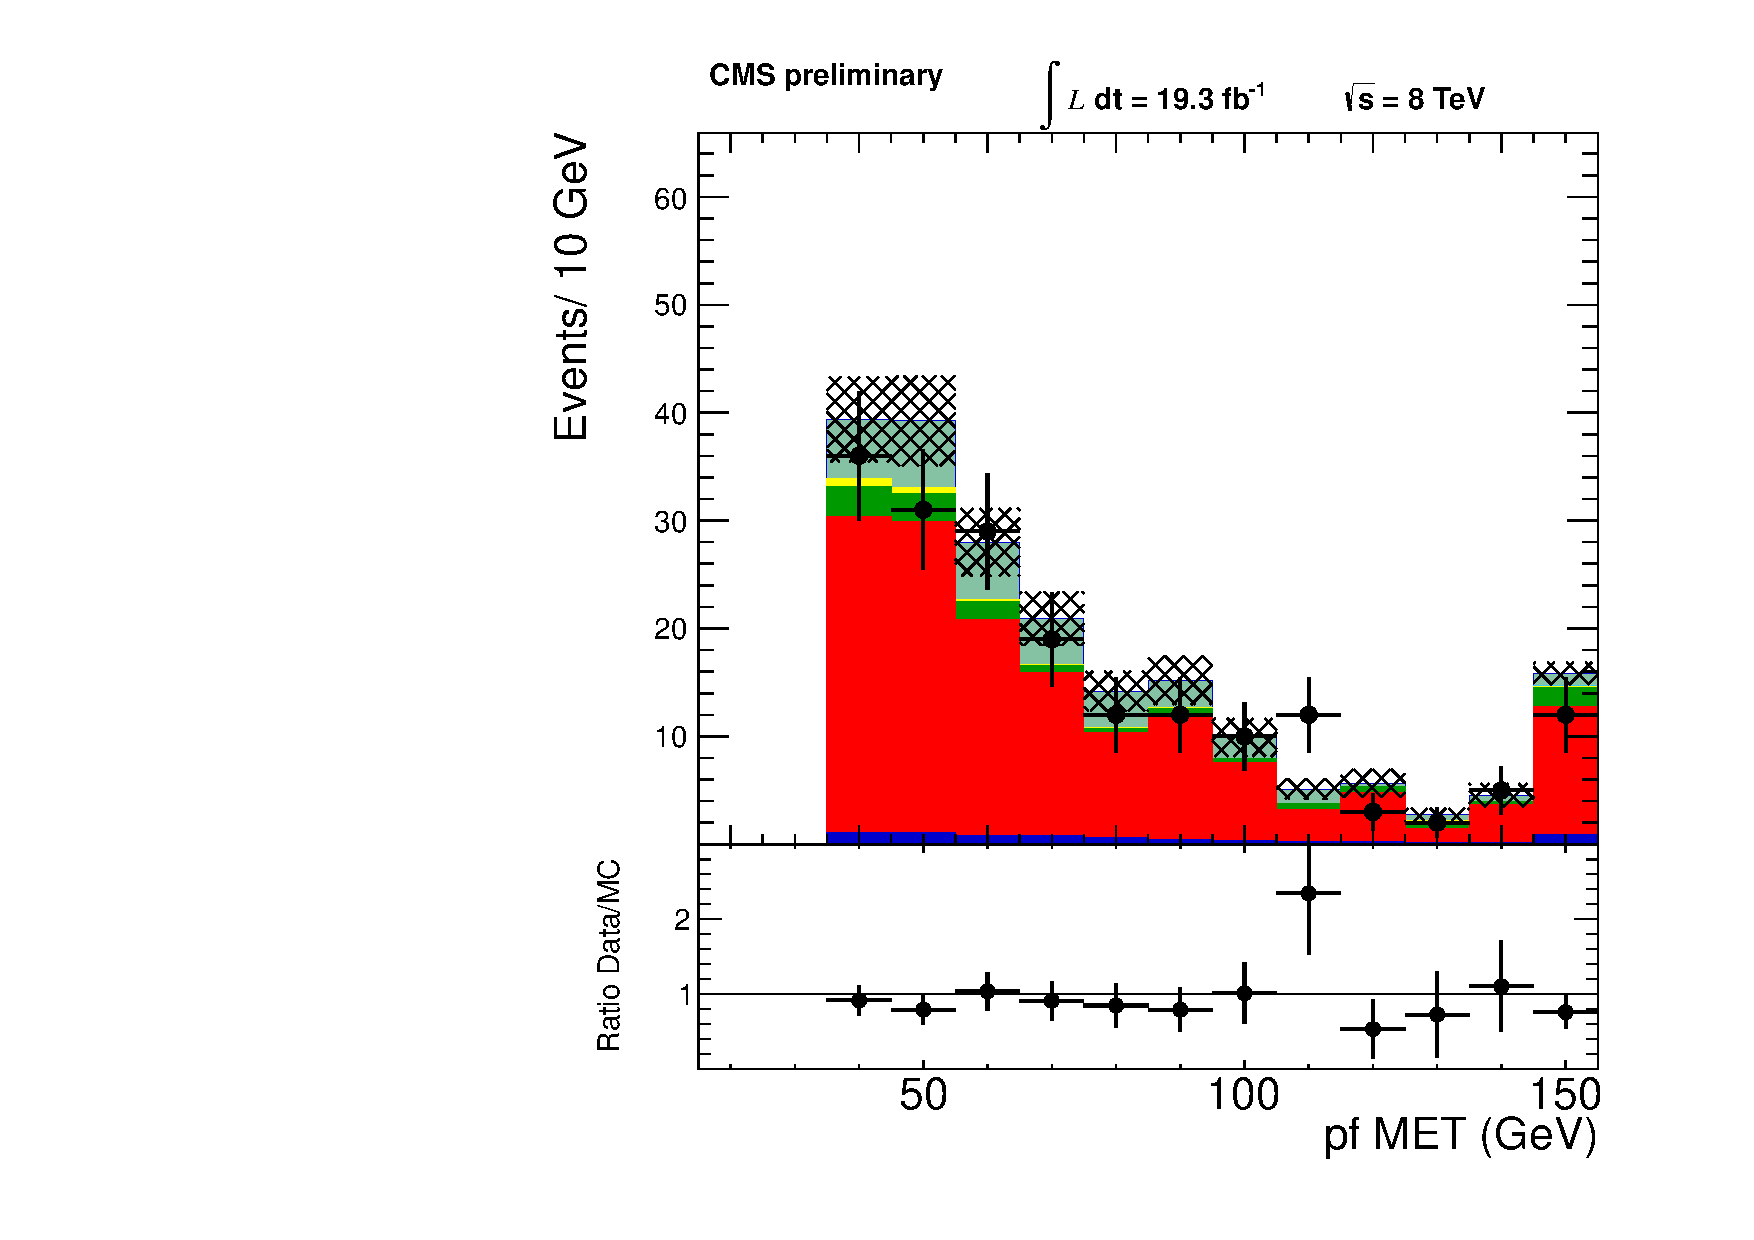
\includegraphics[width=.32\textwidth]{figs/mu_event_met_pfmet.pdf}
}   
%\subfigure[]{
%   \includegraphics[width=.32\textwidth]{figs/mu_W_mt1.pdf}
%}   
\subfigure[]{
   \includegraphics[width=.32\textwidth]{figs/mu_mlvjja1.pdf}
}   \\
\subfigure[]{
   \includegraphics[width=.32\textwidth]{figs/el_event_met_pfmet.pdf}
}   
%\subfigure[]{
%   \includegraphics[width=.32\textwidth]{figs/el_W_mt1.pdf}
%}   
\subfigure[]{
   \includegraphics[width=.32\textwidth]{figs/el_mlvjja1.pdf}
}   
\caption{Data and MC comparison plots for muon channel \MET (a)  $M_{lvjj\gamma}$ (b);
electron channel \MET (c) $M_{lvjj\gamma}$ (d)}
\label{eldijetplots}
\end{center}
\end{figure}

Event yield is summarized in Table \ref{tab:evt}.

\begin{table}[htb]
\centering
\scalebox{1.15}{
  \begin{tabular}{|c|c|c|}
  \hline
  Process  & muon channel & electron channel  \\
    & number of events & number of events  \\
  \hline
  \hline
  W$\gamma$+jets                   & 136.9 $\pm$ 3.5  $\pm$ 9.2  $\pm$ 0.0  & 101.6 $\pm$ 2.9 $\pm$ 8.0 $\pm$ 0.0  \\
  WV+jet, jet$\rightarrow \gamma$  & 33.1  $\pm$ 1.3  $\pm$ 4.6  $\pm$ 0.0  & 21.3  $\pm$ 1.0 $\pm$ 3.1 $\pm$ 0.0  \\
  MC t$\overline{t}\gamma$         & 12.5  $\pm$ 0.8  $\pm$ 2.9  $\pm$ 0.5  & 9.1   $\pm$ 0.7 $\pm$ 2.1 $\pm$ 0.4  \\
  MC single top                    & 2.8   $\pm$ 0.8  $\pm$ 0.2  $\pm$ 0.1  & 1.7   $\pm$ 0.6 $\pm$ 0.1 $\pm$ 0.1  \\
  MC Z$\gamma$+jets                & 1.7   $\pm$ 0.1  $\pm$ 0.1  $\pm$ 0.1  & 1.5   $\pm$ 0.1 $\pm$ 0.1 $\pm$ 0.1  \\
  multijets                        & $<$0.2$\pm$ 0.0  $\pm$ 0.1  $\pm$ 0.0  & 7.2   $\pm$ 3.6 $\pm$ 3.6 $\pm$ 0.0  \\
  \hline
  SM WW$\gamma$                    & 6.3   $\pm$ 0.1  $\pm$ 1.5  $\pm$ 0.3  & 4.7   $\pm$ 0.1 $\pm$ 1.1 $\pm$ 0.2  \\
  SM WZ$\gamma$                    & 0.6   $\pm$ 0.0  $\pm$ 0.1  $\pm$ 0.0  & 0.5   $\pm$ 0.0 $\pm$ 0.1 $\pm$ 0.0  \\
  \hline
  Total predicted                  & 193.9 $\pm$ 3.9 $\pm$ 10.8  $\pm$ 1.0  & 147.6 $\pm$ 4.8 $\pm$ 9.6 $\pm$ 0.7  \\
  \hline
  \hline
  Data                             & 183                                    & 139     \\
  \hline
  \end{tabular}}
  \caption{Expected number of events per process, with statistical, systematic and luminosity uncertainties quoted.}
  \label{tab:evt}
\end{table}


%%%%%%%%%%%%%%%%%%%%%%%%%%%%%%%%%%%%%%%%%%%%%%%%%%%%%%%%%%%%%%%%%%%%%%%%%%
%%%%%%%%%%%%%%%%%%%%%%%%%%%%%%%%%%%%%%%%%%%%%%%%%%%%%%%%%%%%%%%%%%%%%%%%%%
\clearpage{}
\section{Selection optimization - MVA}
\label{sec:MVA}
% ---- ---- ---- ---- ---- ---- ---- ---- ---- ---- ---- ---- ---- ---- ----

We have considered a multi-variate approach to further improve the signal and background separation in the analysis. It is performed by combining several observables into a Boosted Decision 
Trees (BDT) using the TMVA analysis package \cite{TMVA}. Two sets of BDT are used, depending on the purpose - search for $WW\gamma$ or aQGC signal. Additionally we do 
differentiation between muon and electron channels. That results in total of four BDTs. As a signal we use MC sample of SM $WW\gamma$ or aQGC with 
$a_{0}^{W}/\Lambda^{2}=-3.10^{5} GeV^{-2}$. As background are used MC $W\gamma+jets$ and data driven fake photon samples. Relative weight of those samples represent their 
contribution to the observed rate in the data. MC samples, used in the training of the BDTs also include per event pile-up and scale factors weights. Selection of the events 
follows the one described in section ~\ref{sec:reco}, with relaxed $m_{jj}$ cut to increase the statistics, needed for the BDT training process.

For the aQGC BDTs are used the following input variables:
\begin{itemize}
\item lepton transverse momentum 
\item missing transverse energy
\item transverse momentum of the leading central jet
\item transverse momentum of the next-to-leading central jet
\item sum of the transverse energy
\item distance between the two central jets in the $\eta-\phi$ plan
\item azimuthal angle between the two central jets
\item azimuthal angle between the photon and lepton
\item azimuthal angle between the photon and missing transverse energy
\item di-jet invariant mass.
\end{itemize}

Input variables distributions for aQGC BDT are shown in Figure~\ref{fig:InAQGCmu} for the muon channel. Distributions for electron channel are similar.

\begin{figure}[]
  \begin{center}
    \subfloat{
    \includegraphics[width=0.9\textwidth]{figs/variables_aQGC_c1.pdf}
  }\\
  \subfloat{
    \includegraphics[width=0.9\textwidth]{figs/variables_aQGC_c2.pdf}
  }
    \caption{ Input variables distributions for aQGC BDT }
    \label{fig:InAQGCmu}
  \end{center}
\end{figure}

The linear correlations between the input variables for signal and background are shown in Figure~\ref{fig:corrAQGCmu} for aQGC BDT muon channel.

\begin{figure}[]
  \begin{center}
    \subfloat{
    \includegraphics[width=0.4\textwidth]{figs/CorrelationMatrixS_aQGC.pdf}
  }
  \subfloat{
    \includegraphics[width=0.4\textwidth]{figs/CorrelationMatrixB_aQGC.pdf}
  }
    \caption{ The linear correlations between the input variables for signal and background for aQGC BDT muon channel. }
    \label{fig:corrAQGCmu}
  \end{center}
\end{figure}

The data-MC comparison for the aQGC MVA output is shown on Figure ~\ref{fig:outaQGCmu}

\begin{figure}[b]
  \begin{center}
    \subfigure[]{
    \includegraphics[width=0.4\textwidth]{figs/mu_mva2jWWAmuA11.pdf}
  }
  \subfigure[]{
    \includegraphics[width=0.4\textwidth]{figs/el_mva2jWWAelA11.pdf}
  }
    \caption{ Data-MC comparison for the aQGC MVA output of (a) muon and (b) electron channel. }
    \label{fig:outaQGCmu}
  \end{center}
\end{figure}

 The cut value on the MVA output is chosen in a way that it keeps very high signal efficiency for events with high photon pT, while provides modest background 
rejections (in the range 30-50%). The singal efficiency is 98$\%$ (97$\%$) for signal events with photon pT larger than 300 GeV(200 GeV).

 
For the SM $WW\gamma$ BDTs are used the following input variables:
\begin{itemize}
\item transverse momentum of the leptonic W
\item distance between the two central jets in the $\eta-\phi$ plan
\item transverse momentum of the leading central jet
\item transverse momentum of the next-to-leading central jet
\item di-jet invariant mass.
\item invariant mass of the $l,\nu,j,j,\gamma$ system
\item transverse momentum of the $l,\nu,j,j,\gamma$ system
\end{itemize}

Input variables distributions for SM $WW\gamma$ BDT are shown in Figure~\ref{fig:InSMmu} for the muon channel. Distributions for electron channel are similar.

\begin{figure}[]
  \begin{center}
    \subfloat{
    \includegraphics[width=0.9\textwidth]{figs/variables_SMWWA_c1.pdf}
  }\\
  \subfloat{
    \includegraphics[width=0.9\textwidth]{figs/variables_SMWWA_c2.pdf}
  }
    \caption{ Input variables distributions for SM $WW\gamma$ BDT }
    \label{fig:InSMmu}
  \end{center}
\end{figure}

The linear correlations between the input variables for signal and background are shown in Figure~\ref{fig:corrSMmu} for SM $WW\gamma$ BDT muon channel.

\begin{figure}[]
  \begin{center}
    \subfloat{
    \includegraphics[width=0.4\textwidth]{figs/CorrelationMatrixS_SMWWA.pdf}
  }
  \subfloat{
    \includegraphics[width=0.4\textwidth]{figs/CorrelationMatrixB_SMWWA.pdf}
  }
    \caption{ The linear correlations between the input variables for signal and background for SM $WW\gamma$ muon channel. }
    \label{fig:corrSMmu}
  \end{center}
\end{figure}

The data-MC comparison for the SM $WW\gamma$ MVA output is shown on Figure ~\ref{fig:outSMmu}

\begin{figure}[]
  \begin{center}
    \subfigure[]{
    \includegraphics[width=0.4\textwidth]{figs/mu_mva2jWWAmuM.pdf}
  }
  \subfigure[]{
    \includegraphics[width=0.4\textwidth]{figs/el_mva2jWWAelM.pdf}
  }
    \caption{ Data-MC comparison for the SM $WW\gamma$ MVA output of (a) muon and (b) electron channel. }
    \label{fig:outSMmu}
  \end{center}
\end{figure}

The signal efficiency vs the background rejection of the SM $WW\gamma$ BDT is shown in Figure~\ref{fig:rocSMmu} . The cut value on the MVA output is chosen in a 
way that it provides 80$\%$ signal efficiency and about 40$\%$ background rejections.

\begin{figure}[]
  \begin{center}
    \includegraphics[width=0.4\textwidth]{figs/rocSM.pdf}
    \caption{ Signal efficiency vs the background rejection of the SM $WW\gamma$ BDT. }
    \label{fig:rocSMmu}
  \end{center}
\end{figure}


\section{Systematic uncertainties}
\label{sec:syst}
We consider several sources of systematic uncertainty, taking into
account their effect on both the signal acceptance and on the template
shapes for the signal extraction fit.  The uncertainty on the
normalization of the backgrounds is taken as part of the statistical
uncertainty.  The largest source of systematic uncertainty is the
shape uncertainty of the W+jets template.  Other sources of systematic
uncertainty considered include jet energy scale (JES) as well as
trigger and lepton identification efficiencies.
%%%%%%%%%%%%%%%%%%%%%%%%%%%%%%%%%%%%%%%%%%%%
\subsection{Systematics due to the W+jets shape}
\label{sec:syst_mjj}
%%%%%%%%%%%%%%%%%%%%%%%%%%%%%%%%%%%%%%%%%%%%%
The $m_{jj}$ shape for W+jets events is taken from the MC.  Its shape
could be different due to NLO corrections and other effects.
Figure~\ref{fig:wjetshapes} shows possible shapes derived from our MC
samples.  To evaluate the effect of these shapes and propagate them
into our limit, we use the five MadGraph samples, which are the large
statistics nominal sample, one sample with the $q^2$ factorization and
renormalization scale doubled, one with the $q^2$ scale halved, one
with the matching scale doubled and one with the matching scale
halved.  We find an ``optimal'' mixture of the MC samples during our
nominal fit and its uncertainty is propagated by the fitter into the
yields and thus into our final limit. %the technique described in
%Section~\ref{sec:wjetsShape} separately for the 2- and 3-jet bins.
%The shapes that are produced corresponding to the different systematic
%variations on the parameters are propagated to the limit setting as a
%systematic error.

%\subsubsection{Uncertainty due to limited amount of MC}
%The main source of systematic error on the W+jets shape is due to the limited amount of MC
%events in the samples. We evaluate this error by producing Toy MC $m_{jj}$ templates
%based on those from the centrally produced sample. The toy templates are passed through the 
%same optimization procedure and a new optimal mixture is obtained. The resulting uncertainty
%on the W$jj$(Diboson) yield is $XX$($XX$) events for the 2-jet bin and $XX$($XX$) events for 
%the $3$-jet bin.
%Using the distributions of the 
%parameters of the mixture we can evaluate the error on those parameters 
%and propagate that error to the limit setting machinery.

%\subsubsection{Uncertainty due to Factorization Scale and ME-PS Matching}
%The fractions of $q^2$ and matching samples in the overall
%(``optimal'') mixture, obtained from the optimization procedure, have
%corresponding uncertainties.  In order to take the $q^2$-matching
%correlations into account it is necessary to perform a scan in both
%dimensions. Specifically, we vary the scaling and matching fractions
%within $\pm 0.2$ of the optimal values. The systematic error on the
%W$jj$ yield is the difference between the value at the minimum
%-loglikelihood ($nll_{Min}$) and the value at $nll_{Min}+1/2$.
%We scan the $nll_{Min}+1/2$ contour and take the largest difference
%(between the W$jj$ yield at the minimum and on the contour) to be the
%systematic error. The scan results are shown in
%Figs.~\ref{fig:NLL2DScan_2j},~\ref{fig:NLL2DScan_3j}.  The error on
%the W$jj$ yield is 153 events (174 events) in the 2-jet (3-jet) bin.
%%%%%%%%%%%%%%%%%%%%%
%\begin{figure}[htb] 
%  {\centering
%    \includegraphics[width=0.49\textwidth]{figs/NLL2DScan_2j_surf.pdf}
%    \includegraphics[width=0.49\textwidth]{figs/NLL2DScan_2j_cont.pdf}
%    \caption{Scan over the relative fractions for $q^2$ and matching in the 2-jet bin: Surface (left) and Contour (right).}
%    \label{fig:NLL2DScan_2j}}
%\end{figure}
%%%%%%%%%%%%%%
%\begin{figure}[htb] 
%  {\centering
%    \includegraphics[width=0.49\textwidth]{figs/NLL2DScan_3j_surf.pdf}
%    \includegraphics[width=0.49\textwidth]{figs/NLL2DScan_3j_cont.pdf}
%    \caption{Scan over the relative fractions for $q^2$ and matching in the 3-jet bin: Surface (left) and Contour (right).}
%    \label{fig:NLL2DScan_3j}}
%\end{figure}
%%%%%%%%%%%%%%
%%%%%%%%%%%%%%%%%%%%%%%%%%%%%%%%%%%%%%%%
%%%%%%%%%%%%%%%%%%%%%%%%%%%%%%%%%%%%%%%%
\subsection{Jet Energy Scale from the hadronic W in top quark events}
\label{sec:topw}
We reconstruct the hadronic W candidate from an almost pure top data control sample. 
The semileptonic top
events are selected by requiring exactly four jets in the event, out of
which two are b-tagged and the other two are anti-btagged. The
hadronic W candidates are formed from two anti-btagged jets. 
The invariant mass of the hadronic W candidates in the muon,
electron, and combined channels are shown in 
Figs.~\ref{fig:topw:mu},~\ref{fig:topw:el}, and 
\ref{fig:topw:muel}, respectively.  When we propagate the difference in the JES to our
templates they make a negligible difference.
%%%%%%%%%%%%%%%%%%%%%
\begin{figure}[htb] 
  {\centering
    \includegraphics[width=0.75\textwidth]{figs/topwjes/top_overlap_mu.pdf}
    \includegraphics[width=0.49\textwidth]{figs/topwjes/top_data_fit_mu.pdf}
    \includegraphics[width=0.49\textwidth]{figs/topwjes/top_mc_fit_mu.pdf}
    \caption{The invariant mass distribution of the hadronic 
      W candidates in the muon semileptonic top sample. 
      The upper plot shows good agreement between the data and MC. 
      We fit the distribution with a Gaussian and extract the peak
      location for the data (left) and MC (right).}
    \label{fig:topw:mu}}
\end{figure}
%%%%%%%%%%%%%%
\begin{figure}[htb] 
  {\centering
    \includegraphics[width=0.75\textwidth]{figs/topwjes/top_overlap_el.pdf}
    \includegraphics[width=0.49\textwidth]{figs/topwjes/top_data_fit_el.pdf}
    \includegraphics[width=0.49\textwidth]{figs/topwjes/top_mc_fit_el.pdf}
    \caption{The invariant mass distribution of the hadronic 
      W candidates in the electron semileptonic top sample. 
      The upper plot shows good agreement between the data and MC. 
      We fit the distribution with a Gaussian and extract the peak
      location for the data (left) and MC (right).}
    \label{fig:topw:el}}
\end{figure}
%%%%%%%%%%%%%
\begin{figure}[htb] 
  {\centering
    \includegraphics[width=0.75\textwidth]{figs/topwjes/top_overlap_muel.pdf}
    \includegraphics[width=0.49\textwidth]{figs/topwjes/top_data_fit_muel.pdf}
    \includegraphics[width=0.49\textwidth]{figs/topwjes/top_mc_fit_muel.pdf}
    \caption{The invariant mass distribution of the hadronic 
      W candidates in the semileptonic top sample (electron and 
      muon combined). 
      The upper plot shows good agreement between the data and MC. 
      We fit the distribution with a Gaussian and extract the peak
      location for the data (left) and MC (right).}
    \label{fig:topw:muel}}
\end{figure}
%%%%%%%%%%%%%%%%%%%%%%%%%%%%%%%%%%%%%%%%%%%%%%%%%%%%%%%%%%%%%%%%%%%%%%%%%%%
%--------------------------------------------------
\subsection{Lepton selection and trigger efficiency}
\label{sec:LeptonSelectionAndTriggerEfficiency}
%%The lepton trigger and selection is common among several CMS analyses and 
%%we benefit from common studies based on tag-and-probe techniques. 
%%
Systematic uncertainties in the trigger efficiencies in Section~\ref{sec:trigger}
are of the order of 1\%. Systematic uncertainties in the lepton reconstruction
and identification efficiency scale factors are of the order of 2\%. These uncertainties
are accounted for in the final systematics that are input to the limit setter.
%--------------------------------------------------
\subsection{MET uncertainty}
MET directly affects our signal acceptance. 
The uncertainty prescription is discussed in Ref.~\cite{met}.
%https://twiki.cern.ch/twiki/bin/viewauth/CMS/MissingETUncertaintyPrescription
In addition, the MET distribution in the data is $\simeq$3\% wider 
than the MC, and placing a hard MET$>30.0$ cut creates an uncertainty. 
We estimate it by smearing the MET for each event by a Gaussian with 
a $\sigma =0.03*$MET and observing how many events pass the cut. 
Specifically, (Events Passing After Smearing)/(Events Passing Before Smearing) 
=0.998 for both muons and electrons.
%%%%%%%%%%%%%%%%%%%%%%%%%%%%
\subsection{Cross-section of nuisance backgrounds}
The uncertainty in the the cross sections of other backgrounds 
like $\ttbar$,  single top, QCD multi-jets, and Z+jets processes 
is already propagated by letting their normalization (i.e., yield) 
float in the fit within a constraint.
%%%%%%%%%%%%%%%%%%%%%%%%%%%%
\subsection{Luminosity uncertainty}
The latest recommendation for the uncertainty on LHC luminosity is 4.5$\%$~\cite{lumiPAS}.
We propagate this uncertainty to the expected yield of the New Physics 
signal while setting limits.
%%%%%%%%%%%%%%%%%%%%%%%%%%%%

%%%%%%%%%%%%%%%%%%%%%%%%%%%%%%%%%%%%%%%%%%%%%%%%%%%%%%%%%%%%%%%%%%%%%%%%%%
%%%%%%%%%%%%%%%%%%%%%%%%%%%%%%%%%%%%%%%%%%%%%%%%%%%%%%%%%%%%%%%%%%%%%%%%%%
\clearpage{}
\section{WW$\gamma$/WZ$\gamma$ cross section measurement}
\label{sec:sys}
% ---- ---- ---- ---- ---- ---- ---- ---- ---- ---- ---- ---- ---- ---- ----
%A measurement of the WW$\gamma$/WZ$\gamma$ cross section is derived using
%
%\begin{center}
%\begin{equation}
%   \sigma = \frac{N_{data}-N_{bkg}}{L \cdot A \cdot \varepsilon_{MC} \cdot SF}
%\label{eq:xsection}
%\end{equation}
%\end{center}
%
%where $\sigma$ is the measured cross section, $N_{data}$ is the number of
%selected events observed in data, $N_{bkg}$ is the number of selected 
%background events predicted from Monte Carlo, L is the integrated 
%luminosity, A is the signal acceptance predicted from Monte Carlo, 
%$\varepsilon_{MC}$ is the Monte Carlo event selection efficiency, and SF 
%is the efficiency scale factor between data and Monte Carlo 
%($\frac{\varepsilon_{data}}{\varepsilon_{MC}}$), such as those listed for
%the photon in Table~\ref{tab:photon_eff}.  Each of these values has an 
%associated systematic and statistical error that must be propagated 
%through equation~\ref{eq:xsection}.  Using standard error propagation, 
%the uncertainty in the cross sectional measurement is derived using
%
%\begin{center}
%\begin{equation}
%  \delta\sigma = |\sigma|\sqrt{(\frac{{\delta}N_{sig}}{N_{sig}})^{2}+(\frac{{\delta}L}{L})^{2}+(\frac{{\delta}A}{A})^{2}+(\frac{\delta\varepsilon_{MC}}{\varepsilon_{MC}})^{2}+(\frac{{\delta}SF}{SF})^{2}}
%\label{eq:xsec_unc}
%\end{equation}
%\end{center}

%where $N_{sig}$ = $N_{data}-N_{bkg}$ and thus

%\begin{center}
%\begin{equation}
%   {\delta}N_{sig} = \sqrt{({\delta}N_{data})^{2}+({\delta}N_{bkg})^{2}}.
%\end{equation}
%\end{center}

%With equations~\ref{eq:xsection} and \ref{eq:xsec_unc}, Table~\ref{tab:xsec_num} lists the values used to measure the WW$\gamma$ cross section.

%\begin{table}[htb]
%\centering
%\scalebox{0.70}{
%  \begin{tabular}{|c|c|c|c|}
%  \hline
%  Variable & Value & Systematic Uncertainty & Statistical Uncertainty \\
%  \hline
%  \hline
%  $N_{data}$                          & 98.0 & ----   & 9.9   \\
%  $N_{bkg}$                           & 112.6 & 9.7   & 4.7   \\
%  L                                   & 19.3  & ----   & 0.6    \\
%  A $\cdot \varepsilon_{MC} \cdot$ SF & 0.004 & 0.0002 & 0.0002 \\
%  \hline
%  \end{tabular}}
%  \caption{List of values and uncertainties used in measuring the WW$\gamma$ cross section.}
%  \label{tab:xsec_num}
%\end{table}

%Using the values in Table~\ref{tab:xsec_num}, the measured cross section for WW$\gamma$ is $\sigma$ = -168.4 $\pm$ 112.9 (Sys.) $\pm$ 127.0 (Stat.) fb.  This measurement takes into account the K-factors used for WW$\gamma$/WZ$\gamma$ and W$\gamma$+Jets processes listed in Section~\ref{sec:Kfact}, as well as the MVA discussed in Section~\ref{sec:MVA}.  The theoretical cross section provided by MadGraph 5 for semileptonic WW$\gamma$ is 41 fb, again taking into account the K-factor for WW$\gamma$ listed in Section~\ref{sec:Kfact}~\cite{MadGraph}.

This SM cross sectional measurement's uncertainties are large due to the low signal 
statistics, the uncertainties in the K-factors used, and the fake photon 
rate's systematic uncertainty of 12-39\%; therefore, we cannot claim an 
observation of WW$\gamma$ events.

The Standard Model WW$\gamma$/WZ$\gamma$ signal strength with and without
MVA optimization is shown in Figure~\ref{fig:signalstrength}, with the 
1-$\sigma$ and 2-$\sigma$ bands. Figure~\ref{fig:signalstrength} 
demonstrates that a signal strength below 1 suggests we are sensitive to 
the signal and can measure the cross section; however, we are well above 
a value of 1 and are therefore not sensitive to the SM signal. It can be 
seen that MVA optimization makes a small improvement on our sensitivity,
and optimizes our sensitivity at a MVA cut of 0.2. 
While the MVA selection helps to improve sensitivity of the measurement it is not changing the fact that only a upper cross section limit is derived for $WV\gamma$. 
Thus we consider the $WV\gamma$ upper cross section limit without use of MVA as the primary result and keep the study documented for future iterations of the analysis.

\begin{figure}[h]
  \begin{center}
    \includegraphics[width=0.75\textwidth]{figs/WVAsignalstrength.pdf}
    \caption{Standard Model WW$\gamma$/WZ$\gamma$ signal strength with various MVA cut values. A strength at or below 1 suggests we are sensitive to the SM signal.}
    \label{fig:signalstrength}
  \end{center}
\end{figure}



%%%%%%%%%%%%%%%%%%%%%%%%%%%%%%%%%%%%%%%%%%%%%%%%%%%%%%%%%%%%%%%%%%%%%%%%%%
%%%%%%%%%%%%%%%%%%%%%%%%%%%%%%%%%%%%%%%%%%%%%%%%%%%%%%%%%%%%%%%%%%%%%%%%%%
\clearpage{}
\section{AQGC parametrization and limits}
\label{sec:aQGClim}
% ---- ---- ---- ---- ---- ---- ---- ---- ---- ---- ---- ---- ---- ---- ----

\subsection{Parametrizations}
In order to set limits on anomalous couplings, we compare the observed 
signal data's kinematics to those of anomalous signal Monte Carlo.  This 
process can involve generating many different Monte Carlo samples for 
various values of each anomalous quartic coupling parameter, or we could 
quantize how anomalous couplings affect certain observable kinematical 
distributions such as photon $p_{T}$ or WW$\gamma$ invariant mass.  

In order to quantize the affect each coupling parameter has on a kinematical
distribution, say photon $p_{T}$, we still generate a few Monte Carlo 
samples for each anomalous coupling parameter, where the parameter of 
interest is varied to multiple values and all other coupling parameters set 
to their standard model value.  For example, we have five quadratic coupling
parameters $\frac{a_{0}^{W}}{\Lambda^{2}}, \frac{a_{C}^{W}}{\Lambda^{2}}, 
\frac{f_{T,0}}{\Lambda^{4}}, \frac{\kappa_{0}^{W}}{\Lambda^{2}}$, and 
$\frac{\kappa_{C}^{W}}{\Lambda^{2}}$.  In 
order to parametrize the affect the parameter 
$\frac{a_{0}^{W}}{\Lambda^{2}}$ has on photon $p_{T}$, we vary this 
parameter's values while fixing $\frac{a_{C}^{W}}{\Lambda^{2}}, 
\frac{f_{T,0}}{\Lambda^{4}}, \frac{\kappa_{0}^{W}}{\Lambda^{2}}, $and$ 
\frac{\kappa_{C}^{W}}{\Lambda^{2}}$ to their
Standard Model values of zero.

In addition to the Standard Model sample, we generate six Monte Carlo AQGC 
samples for variation in each parameter.  Then, after applying event 
selection cuts described in sections~\ref{sec:evtSel} and~\ref{sec:photon}, 
efficiency and pileup weights, and the photon $p_{T}$-dependent k-factor 
described in section~\ref{sec:Kfact}, each sample's photon $p_{T}$ 
distribution is divided by the standard model photon $p_{T}$ distribution to
form a AQGC/SM ratio for each photon $p_{T}$ bin. A quadratic distibution is
formed by plotting each AQGC/SM ratio value for a specific photon $p_{T}$ 
bin, as can be seen in Figure~\ref{fig:para_ptbins} for 
$\frac{a_{0}^{W}}{\Lambda^{2}}$ in the muon channel. 
Figure~\ref{fig:para_ptbins}-(a) exhibits a quadratic fit that decreases
with increasing AQGC: (1) this is only found to happen with $a_{0}^{W}$
and with this binning and (2) it is allowed because the limits for this
parameter fall within the fit's range and thus we benefit from minimizing
$\chi^{2}$.

\begin{figure}[]
  \begin{center}
    \subfigure[]{
    \includegraphics[width=0.33\textwidth]{figs/a0W_PhotonPT_para_bin1.png}
  }
    \subfigure[]{
    \includegraphics[width=0.33\textwidth]{figs/a0W_PhotonPT_para_bin2.png}
  }
    \subfigure[]{
    \includegraphics[width=0.33\textwidth]{figs/a0W_PhotonPT_para_bin3.png}
  }\\
    \subfigure[]{
    \includegraphics[width=0.33\textwidth]{figs/a0W_PhotonPT_para_bin4.png}
  }
    \subfigure[]{
    \includegraphics[width=0.33\textwidth]{figs/a0W_PhotonPT_para_bin5.png}
  }
    \subfigure[]{
    \includegraphics[width=0.33\textwidth]{figs/a0W_PhotonPT_para_bin6.png}
  }\\
    \subfigure[]{
    \includegraphics[width=0.33\textwidth]{figs/a0W_PhotonPT_para_bin7.png}
  }
    \subfigure[]{
    \includegraphics[width=0.33\textwidth]{figs/a0W_PhotonPT_para_bin8.png}
  }
    \subfigure[]{
    \includegraphics[width=0.33\textwidth]{figs/a0W_PhotonPT_para_bin9.png}
  }\\
    \subfigure[]{
    \includegraphics[width=0.33\textwidth]{figs/a0W_PhotonPT_para_bin10.png}
  }
    \caption{AQGC/SM ratio values for each $a_{0}^{W}/\Lambda^{2}$ Monte Carlo sample (muon channel) within each of the following Photon $p_{T}$ bins: Photon $p_{T}$ bins (a) 30-72 GeV, (b) 72-114 GeV, (c) 114-156 GeV, (d) 156-198 GeV, (e) 198-240 GeV, (f) 240-282 Gev, (g) 282-324 GeV, (h) 324-366 GeV, (i) 366-408 GeV, 408-inf. GeV (overflow bin)}
  \label{fig:para_ptbins}
  \end{center}
\end{figure}

We fit this quadratic distribution with a quadratic function that can later 
be used to predict the AQGC/SM ratio value for any arbitrary anomalous 
coupling value for that specific coupling parameter and photon $p_{T}$ bin. 
It can even been seen in Figure~\ref{fig:para_ptbins} that the overflow 
photon $p_{T}$ bin has a quadratic behavior in AQGC and thus can be 
parametrized.  

Keeping in mind that the AQGC/SM ratio fit function for a given coupling 
parameter is a function of the coupling parameter's value and depends on the
photon $p_{T}$ bin, we then plot and fit the coefficients of the AQGC/SM 
quadratic fit function versus photon $p_{T}$ in order to obtain the 
$p_T{}$-dependence of the AQGC/SM ratio.  Therefore, we obtain a 
parametrization of the affect each anomalous coupling parameter has on 
photon $p_{T}$ by substituting the $p_{T}$-dependent coefficient fit 
functions into the coupling parameter-dependent AQGC/SM ratio fit function, 
as shown in equation~\ref{parameq}.

\begin{center}
\begin{equation}
R(parameter,p_{T}) = \frac{\# AQGC events(parameter,p_{T})}{\# SM events(p_{T})} = 1 + C_{0}(p_{T}) \cdot parameter + C_{1}(p_{T}) \cdot parameter^{2}
\label{parameq}
\end{equation}
\end{center}

A closure test can be performed using equation~\ref{parameq} as a 
reweighting function applied to the Standard Model photon $p_{T}$ spectrum, 
as can be seen in Figure~\ref{fig:para_closure} for 
$\frac{a_{0}^{W}}{\Lambda^{2}}$ where the simulated (parametrized) Monte 
Carlo is compared to the generated (true) Monte Carlo.  Furthermore, the 
ratio between some of the simulated and generated Monte Carlo of each AQGC 
parameter can be seen in Figure~\ref{fig:para_closure_ratio}, where the 
deviation in each photon $p_{T}$ bin remains below 40\%.  The deviation in 
the overflow photon $p_{T}$ bin for each AQGC parameter remains below 15\% 
as well. A closure test ratio plot is also included in
Figure~\ref{fig:para_closure_ratio} for $\frac{a_{0}^{W}}{\Lambda^{2}}$ when using
a form factor of $\Lambda = 500 GeV, n = 2$.

\begin{figure}[]
  \begin{center}
    \subfigure[]{
    \includegraphics[width=0.45\textwidth]{figs/a0W_p5_closure.png}
  }
    \subfigure[]{
    \includegraphics[width=0.45\textwidth]{figs/a0W_m5_closure.png}
  }
    \caption{Photon $p_{T}$ of simulated (Red line) and generated (Blue line) Monte Carlo samples for (a) $a_{0}^{W}/\Lambda^{2}$ = 5E-05 $GeV^{-2}$ and (b) $a_{0}^{W}/\Lambda^{2}$ = -5E-05 $GeV^{-2}$ (both are muon channel)}
  \label{fig:para_closure}
  \end{center}
\end{figure}

\begin{figure}[]
  \begin{center}
    \subfigure[]{
    \includegraphics[width=0.45\textwidth]{figs/a0W_ratio.png}
  }
    \subfigure[]{
    \includegraphics[width=0.45\textwidth]{figs/acW_ratio.png}
  }\\
    \subfigure[]{
    \includegraphics[width=0.45\textwidth]{figs/lt0_ratio.png}
  }
    \subfigure[]{
    \includegraphics[width=0.45\textwidth]{figs/aQGC_K0W_closure_ratio.png}
  }\\
    \subfigure[]{
    \includegraphics[width=0.45\textwidth]{figs/aQGC_KCW_closure_ratio.png}
  }
    \subfigure[]{
    \includegraphics[width=0.45\textwidth]{figs/a0W_500FFn2_ratio.png}
  }
    \caption{Muon channel Simulated:Generated ratio as a function of photon $p_{T}$ for (a) $a_{0}^{W}/\Lambda^{2}$ = -5E-05 $GeV^{-2}$ (Red line), 5E-05 $GeV^{-2}$ (Blue line); (b) $a_{C}^{W}/\Lambda^{2}$ = -8E-05 $GeV^{-2}$ (Red line), 8E-05 $GeV^{-2}$ (Blue line); (c) $f_{T,0}/\Lambda^{4}$ = -8E-11 $GeV^{-2}$ (Red line), 8E-11 $GeV^{-2}$ (Blue line); (d) $\kappa_{0}^{W}/\Lambda^{2}$ = -2E-5 $GeV^{-2}$ (Red line), 2E-5 $GeV^{2}$ (Blue line); (e) $\kappa_{C}^{W}/\Lambda^{2}$ = -3E-5 $GeV^{-2}$ (Red line), 3E-5 $GeV^{2}$ (Blue line); (f) $a_{0}^{W}/\Lambda^{2}$ = -140E-05 $GeV^{-2}$ (Red line), 140E-05 $GeV^{-2}$ (Blue line) incorporating a Form Factor of $\Lambda = 500 GeV, n = 2$.}
  \label{fig:para_closure_ratio}
  \end{center}
\end{figure}

\newpage
\subsection{Limits using Photon $p_{T}$}
\label{sec:limits_pT}
We use the photon $p_T$ distribution as observable to set limit on anomalous
couplings.

We use the ``Higgs Combination'' package \cite{cite:combine} for
setting exclusion limits. This package is a
RooStats\cite{cite:roostats}-based statistical analysis tool-set
recommended by the CMS Higgs PAG and approved by CMS statistics committee.

We take as inputs the photon $p_T$ distributions for each signal model 
(\textit{i.e.}, various choices of $a_{0}^{W}/\Lambda^{2}$,  
$a_{C}^{W}/\Lambda^{2}$, $f_{T,0}/\Lambda^{4}$, $\kappa_{0}^{W}/\Lambda^{2}$, and 
$\kappa_{C}^{W}/\Lambda^{2}$), data, and total background that survive after
analysis cuts. All of these distributions are segregated by lepton flavor,
which represent independent channel inputs to the limit setter. 
Figure~\ref{fig:limitinput} shows the muon channel for given values of AQGC 
parameters, with and without MVA optimization (cut at 0.5), in which the AQGC input is the 
excess events from the SM prediction. For the MVA case in Figure~\ref{fig:limitinput},
the $f_{T,0}/\Lambda^{4}$ sample had diminished statistics after the cut on the MVA output
was made. We supply these distributions over the 
range $30-450~\GeV/c$ in the form of histograms to the limit setter. The binning 
is chosen such that the left-most bin begins at the first 2012 dataset point, and the 
right-most bin begins just beyond the last 2012 dataset point. We extend the
right-most bin to be an overflow bin, and since it begins just beyond the
reach of 2012 data in our events, it represents physics beyond our
sensitivity.

\begin{figure}[b]
  \begin{center}
    \subfigure[]{
      \includegraphics[width=0.45\textwidth]{figs/mu_limit_input.pdf}
    }
    \subfigure[]{
      \includegraphics[width=0.45\textwidth]{figs/mu_limit_input_MVA.pdf}
    }
    \caption{ Input photon $p_{T}$ distributions for the limit setter of the muon channel (a) without MVA optimization and (b) with MVA optimization, cut at 0.5: SM prediction (Black); AQGC excess from SM prediction for $a_{0}^{W}/\Lambda^{2}$ (Red), $a_{C}^{W}/\Lambda^{2}$ (Green), $f_{T,0}/\Lambda^{4}$ (Blue), $\kappa_{0}^{W}/\Lambda^{2}$ (Orange), and $\kappa_{C}^{W}/\Lambda^{2}$ (Violet). }
    \label{fig:limitinput}
  \end{center}
\end{figure}

The limit setter is then set to utilize the ``ProfileLikelihood CL$_{s}$''
\cite{cite:asympcls1,cite:asympcls2} method. Figure~\ref{fig:limitshape1d_noMVA} 
is the resulting shape-based observed 
and expected exclusion limits without MVA optimization discussed in 
Section~\ref{sec:MVA}.  Exclusion limits for $a_{0}^{W}/\Lambda^{2}$, 
$a_{C}^{W}/\Lambda^{2}$, $f_{T,0}/\Lambda^{4}$, $\kappa_{0}^{W}/\Lambda^{2}$, and 
$\kappa_{C}^{W}/\Lambda^{2}$ are computed at the 95\% CL and are listed in
Table~\ref{tab:limit_values_noMVA} for the analysis without MVA optimization
discussed in Section~\ref{sec:MVA}. Table~\ref{tab:limit_values_noMVA_dim8}
contains the transformed Dimension 8 limits from the Dimension 6 a$_{0}^{W}$
and a$_{C}^{W}$ parameters, without MVA optimization. 

\begin{table}[htb]
\centering
\scalebox{1.0}{
  \begin{tabular}{|c|c|}
  \hline
  Observed Limits & Expected Limits \\
  \hline
  \hline
  -21 ($TeV^{-2}$) $<$ $a_{0}^{W}/\Lambda^{2}$ $<$ 20 ($TeV^{-2}$)  & -24 ($TeV^{-2}$) $<$ $a_{0}^{W}/\Lambda^{2}$ $<$ 23 ($TeV^{-2}$) \\
  -34 ($TeV^{-2}$) $<$ $a_{C}^{W}/\Lambda^{2}$ $<$ 32 ($TeV^{-2}$)  & -37 ($TeV^{-2}$) $<$ $a_{C}^{W}/\Lambda^{2}$ $<$ 34 ($TeV^{-2}$) \\
  -25 ($TeV^{-4}$) $<$ $f_{T,0}/\Lambda^{4}$ $<$ 24 ($TeV^{-4}$)  & -27 ($TeV^{-4}$) $<$ $f_{T,0}/\Lambda^{4}$ $<$ 27 ($TeV^{-4}$) \\
  -12 ($TeV^{-2}$) $<$ $\kappa_{0}^{W}/\Lambda^{2}$ $<$ 10 ($TeV^{-2}$)  & -12 ($TeV^{-2}$) $<$ $\kappa_{0}^{W}/\Lambda^{2}$ $<$ 12 ($TeV^{-2}$) \\
  -18 ($TeV^{-2}$) $<$ $\kappa_{C}^{W}/\Lambda^{2}$ $<$ 17 ($TeV^{-2}$)  & -19 ($TeV^{-2}$) $<$ $\kappa_{C}^{W}/\Lambda^{2}$ $<$ 18 ($TeV^{-2}$) \\
  \hline
  \end{tabular}}
  \caption{95\% CL shape-based exclusion limits listed for both the muon and electron channels of each AQGC parameter without MVA optimization, using photon $p_{T}$.}
  \label{tab:limit_values_noMVA}
\end{table}

\begin{table}[htb]
\centering
  \scalebox{1.0}{
  \begin{tabular}{|c|c|}
  \hline
  Observed Limits & Expected Limits \\
  \hline
  \hline
  -77 (TeV$^{-4}$) $<$ $f_{M,0}/\Lambda^{4}$ $<$ 81 (TeV$^{-4}$)  & -89 (TeV$^{-4}$) $<$ $f_{M,0}/\Lambda^{4}$ $<$ 93 (TeV$^{-4}$) \\
  -131 (TeV$^{-4}$) $<$ $f_{M,1}/\Lambda^{4}$ $<$ 123 (TeV$^{-4}$)    & -143  (TeV$^{-4}$) $<$ $f_{M,1}/\Lambda^{4}$ $<$ 131  (TeV$^{-4}$) \\
  -39 (TeV$^{-4}$) $<$ $f_{M,2}/\Lambda^{4}$ $<$ 40 (TeV$^{-4}$)  & -44 (TeV$^{-4}$) $<$ $f_{M,2}/\Lambda^{4}$ $<$ 46 (TeV$^{-4}$) \\
  -66 (TeV$^{-4}$) $<$ $f_{M,3}/\Lambda^{4}$ $<$ 62 (TeV$^{-4}$)    & -71  (TeV$^{-4}$) $<$ $f_{M,3}/\Lambda^{4}$ $<$ 66  (TeV$^{-4}$) \\
  \hline
  \end{tabular}}  \caption{95\% CL shape-based exclusion limits listed for both the muon and electron channels of each Dim. 8 AQGC parameter without MVA optimization, using photon $p_{T}$.}
  \label{tab:limit_values_noMVA_dim8}
\end{table}


\begin{figure}[hb]
  \begin{center}
    \subfigure[]{
    \includegraphics[width=0.45\textwidth]{figs/a0W_PhotonPT_limit_noMVA.pdf}
  }
    \subfigure[]{
    \includegraphics[width=0.45\textwidth]{figs/acW_PhotonPT_limit_noMVA.pdf}
  }\\
  \subfigure[]{
    \includegraphics[width=0.45\textwidth]{figs/LT0_PhotonPT_limit_noMVA.pdf}
  }
  \subfigure[]{
    \includegraphics[width=0.45\textwidth]{figs/K0W_PhotonPT_limit_noMVA.pdf}
  }\\
  \subfigure[]{
    \includegraphics[width=0.45\textwidth]{figs/KCW_PhotonPT_limit_noMVA.pdf}
  }
  \subfigure[]{
    \includegraphics[width=0.45\textwidth]{figs/a0W_PhotonPT_limit_noMVA_500FFn2.pdf}
  }
    \caption{ Exclusion limits for (a) $a_{0}^{W}/\Lambda^{2}$; (b) $a_{C}^{W}/\Lambda^{2}$; (c) $f_{T,0}/\Lambda^{4}$; (d) $\kappa_{0}^{W}/\Lambda^{2}$; (e) $\kappa_{C}^{W}/\Lambda^{2}$; (f) $a_{0}^{W}/\Lambda^{2}$ with Form Factor $\Lambda = 500 GeV, n = 2$, all at the 95\% CL and no MVA optimization, using photon $p_{T}$.}
    \label{fig:limitshape1d_noMVA}
  \end{center}
\end{figure}


\subsection{Limits using M$_{WW\gamma}$}
\label{sec:limits_Mlvjja}
As an additional means of setting limits on AQGC, we performed the same
limit setting procedure previously discussed while using the WW$\gamma$
invariant mass as the descriminating distribution. Much like the photon
$p_{T}$ distribution, the $M_{WW\gamma}$ distribution experiences an
increase in the tail end of its spectrum (high-mass region) as a result of
AQGC; however, this distribution experiences much desctructive interefence
in the low mass region ($< 700 GeV/c^{2}$). We obtain a parametrization of 
AQGC as a function of the $a_{0}^{W}/\Lambda^{2}$ parameter
and WW$\gamma$ invariant mass, and Figure~\ref{fig:limits_Mlvjja} shows the 
resulting limits. Table~\ref{tab:limit_values_Mlvjja} lists the observed and expected limits at 
95\% CL We did not perform
MVA optimization in obtaining these limits, as our sensitivity was not
significantly increased by MVA methods (see Section~\ref{sec:limits_MVA}).
The behavior of the observed limits and the existence of destructive
interference makes this distribution not as optimal as photon $p_{T}$.

\begin{table}[htb]
\centering
\scalebox{1.0}{
  \begin{tabular}{|c|c|}
  \hline
  Observed Limits & Expected Limits \\
  \hline
  \hline
  -19 ($TeV^{-2}$) $<$ $a_{0}^{W}/\Lambda^{2}$ $<$ 16 ($TeV^{-2}$)  & -31 ($TeV^{-2}$) $<$ $a_{0}^{W}/\Lambda^{2}$ $<$ 28 ($TeV^{-2}$) \\
  \hline
  \end{tabular}}
  \caption{95\% CL shape-based exclusion limits listed for both the muon and electron channels of the AQGC parameter $a_{0}^{W}/\Lambda^{2}$, using $M_{WW\gamma}$ and without MVA optimization.}
  \label{tab:limit_values_Mlvjja}
\end{table}

\begin{figure}[hb]
  \begin{center}
    \subfigure[]{
    \includegraphics[width=0.45\textwidth]{figs/a0W_Mlvjja_limit_noMVA.pdf}
  }
    \caption{ Exclusion limits for $a_{0}^{W}/\Lambda^{2}$ at 95\% CL and no MVA optimization, using M$_{WW\gamma}$.}
    \label{fig:limits_Mlvjja}
  \end{center}
\end{figure}

\subsection{$a_{0}^{W}$ Limits using MVA}
\label{sec:limits_MVA}
In order to demonstrate the effect of MVA optimization on extracted limits
for one of our parameters, $a_{0}^{W}$, we varied the MVA cut value and
produced the limits shown in Figure~\ref{fig:limits_MVA} and 
Figure~\ref{fig:limits_MVA_FF}. It is shown that
MVA optimization does not improve the extracted limits beyond the original
sigma bands shown in Figure~\ref{fig:limitshape1d_noMVA}. Only the expected
limit is shown to demonstrate the best limits we could achieve. 
Table~\ref{tab:limit_values_MVA} lists the best expected limits from the MVA 
cut scan for the non-Form Factor limits at a MVA cut value of 0.5. 
The minor improvement in the limit do not justify the use of MVA techniques, thus we consider as a primary result the limits without MVA selection optimization.
%Table~\ref{tab:limit_values_MVA_FF} lists the best expected limits from the MVA cut scan for the 
%Form Factor limits at a MVA cut value of 0.1.

\begin{table}[htb]
\centering
\scalebox{1.0}{
  \begin{tabular}{|c|}
  \hline
  Expected Limits \\
  \hline
  \hline
  -24 ($TeV^{-2}$) $<$ $a_{0}^{W}/\Lambda^{2}$ $<$ 21 ($TeV^{-2}$)\\
  \hline
  \end{tabular}}
  \caption{95\% CL shape-based expected limits listed for both the muon and electron channels of the AQGC parameter $a_{0}^{W}/\Lambda^{2}$, using Photon $p_{T}$ and with MVA optimization cut = 0.5.}
  \label{tab:limit_values_MVA}
\end{table}

%\begin{table}[htb]
%\centering
%\scalebox{0.70}{
%  \begin{tabular}{|c|}
%  \hline
%  Expected Limits \\
%  \hline
%  \hline
%  -151 (10 $TeV^{-2}$) $<$ $a_{0}^{W}/\Lambda^{2}$ $<$ 149 (10 $TeV^{-2}$)\\
%  \hline
%  \end{tabular}}
%  \caption{95\% C.L. shape-based expected limits listed for both the muon and electron channels of the aQGC parameter $a_{0}^{W}/\Lambda^{2}$, Form Factor $\Lambda = 500 GeV, n = 2$, using Photon $p_{T}$ and with MVA optimization cut = 0.1.}
%  \label{tab:limit_values_MVA_FF}
%\end{table}

\begin{figure}[hb]
  \begin{center}
    \subfigure[]{
    \includegraphics[width=0.33\textwidth]{figs/a0W_PhotonPT_limit_MVA01.pdf}
  }
    \subfigure[]{
    \includegraphics[width=0.33\textwidth]{figs/a0W_PhotonPT_limit_MVA02.pdf}
  }
    \subfigure[]{
    \includegraphics[width=0.33\textwidth]{figs/a0W_PhotonPT_limit_MVA03.pdf}
  }\\
    \subfigure[]{
    \includegraphics[width=0.33\textwidth]{figs/a0W_PhotonPT_limit_MVA04.pdf}
  }
    \subfigure[]{
    \includegraphics[width=0.33\textwidth]{figs/a0W_PhotonPT_limit_MVA05.pdf}
  }
    \caption{ Exclusion limits for $a_{0}^{W}/\Lambda^{2}$ at 95\% CL and MVA optimization cut at: (a) 0.1, (b) 0.2, (c) 0.3, (d) 0.4, and (e) 0.5, using Photon $p_{T}$.}
    \label{fig:limits_MVA}
  \end{center}
\end{figure}

\begin{figure}[hb]
  \begin{center}
    \subfigure[]{
    \includegraphics[width=0.33\textwidth]{figs/a0W_PhotonPT_limit_MVA01_500FFn2.pdf}
  }
    \subfigure[]{
    \includegraphics[width=0.33\textwidth]{figs/a0W_PhotonPT_limit_MVA02_500FFn2.pdf}
  }
    \subfigure[]{
    \includegraphics[width=0.33\textwidth]{figs/a0W_PhotonPT_limit_MVA03_500FFn2.pdf}
  }
    \caption{ Exclusion limits for $a_{0}^{W}/\Lambda^{2}$ at 95\% CL and MVA optimization cut at: (a) 0.1, (b) 0.2, and (c) 0.3 using Photon $p_{T}$ and Form Factor $\Lambda = 500 GeV, n = 2$.}
    \label{fig:limits_MVA_FF}
  \end{center}
\end{figure}

\subsection{$a_{0}^{W}$ Limits using Photon $p_{T}$-dependent K-Factor}
\label{sec:limits_pTKFact}
In order to verify that our limit setting procedure is not neglecting
possible new physics, we produced a photon $p_{T}$-dependent K-factor
for the parameter $a_{0}^{W}$. Our procedure outlined in 
Section~\ref{sec:aQGC_Kfac} applys a constant Drell-Yan like K-factor
of 1.185 to the resulting spectrum after removing the SM prediction 
of the signal; the limits shown in Figure~\ref{fig:limits_functKfac} are derived
by first applying a AQGC-and-photon-$p_{T}$-dependent K-factor
to the predicted AQGC sample and then removing the SM prediction that
has had its SM 2.1 K-factor applied. 
Figure~\ref{fig:limits_functKfac} and Table~\ref{tab:limit_values_funcKFac}
demonstrate that the effect is minimal.

\begin{table}[htb]
\centering
\scalebox{1.0}{
  \begin{tabular}{|c|c|}
  \hline
  Observed Limits & Expected Limits \\
  \hline
  \hline
  -24 ($TeV^{-2}$) $<$ $a_{0}^{W}/\Lambda^{2}$ $<$ 20 ($TeV^{-2}$)  & -27 ($TeV^{-2}$) $<$ $a_{0}^{W}/\Lambda^{2}$ $<$ 22 ($TeV^{-2}$) \\
  \hline
  \end{tabular}}
  \caption{95\% CL shape-based exclusion limits listed for both the muon and electron channels of the AQGC parameter $a_{0}^{W}/\Lambda^{2}$, using photon $p_{T}$, without MVA optimization, and with a $p_{T}$-dependent K-factor.}
  \label{tab:limit_values_funcKFac}
\end{table}

\begin{figure}[hb]
  \begin{center}
    \subfigure[]{
    \includegraphics[width=0.45\textwidth]{figs/a0W_PhotonPT_limit_noMVA_functKFac.pdf}
  }
    \caption{ Exclusion limits for $a_{0}^{W}/\Lambda^{2}$ at 95\% CL using photon $p_{T}$-dependent functional K-factors.}
    \label{fig:limits_functKfac}
  \end{center}
\end{figure}

\subsection{$a_{0}^{W}$ Limits using $\Lambda = 500 GeV, n = 2$ Form Factor}
In the investigation of unitarity violation, we have also set limits on
$a_{0}^{W}/\Lambda^{2}$ using a form factor of $\Lambda = 500 GeV and n = 2$.
The limits without MVA optimization are shown in Figure~\ref{fig:limitshape1d_noMVA},
with their values listed in Table~\ref{tab:limit_values_noMVA_FF}. Limits with 
various MVA cuts are shown in Figure~\ref{fig:limits_MVA_FF}.

\begin{table}[htb]
\centering
\scalebox{1.0}{
  \begin{tabular}{|c|c|}
  \hline
  Observed Limits & Expected Limits \\
  \hline
  \hline
  -1480 ($TeV^{-2}$) $<$ $a_{0}^{W}/\Lambda^{2}$ $<$ 1500 ($TeV^{-2}$)  & -1530 ($TeV^{-2}$) $<$ $a_{0}^{W}/\Lambda^{2}$ $<$ 1530 ($TeV^{-2}$) \\
  -5782 ($TeV^{-4}$) $<$ $f_{M,0}/\Lambda^{4}$ $<$ 5705 ($TeV^{-4}$)  & -5898 ($TeV^{-4}$) $<$ $f_{M,0}/\Lambda^{4}$ $<$ 5898 ($TeV^{-4}$) \\
  -2891 ($TeV^{-4}$) $<$ $f_{M,2}/\Lambda^{4}$ $<$ 2853 ($TeV^{-4}$)  & -2949 ($TeV^{-4}$) $<$ $f_{M,2}/\Lambda^{4}$ $<$ 2949 ($TeV^{-4}$) \\
  \hline
  \end{tabular}}
  \caption{95\% CL shape-based exclusion limits listed for both the muon and electron channels of each AQGC parameter $a_{0}^{W}/\Lambda^{2}$, with a Form Factor of $\Lambda = 500 GeV, n = 2$, using photon $p_{T}$ and without MVA optimization.}
  \label{tab:limit_values_noMVA_FF}
\end{table}

\newpage
\section{Conclusions}
\label{sec:conclusions}
We have studied the electroweak production 
of two heavy gauge bosons  in events 
with a leptonically decaying W boson and exactly two jets.
The analyzed dataset 
corresponds to an integrated luminosity of 5.0~fb${}^{-1}$ at 
$\sqrt{s} = 7$~TeV collected by the CMS detector at the Large Hadron Collider.
With the kinematic requirements imposed in the analysis, we 
observe 2979 $\pm$ 361 (stat) $\pm$ 402 (syst) WW+WZ events, 
in agreement with the Standard Model expectation. 
The measured value of the sum of WW and WZ cross sections is 
66.7 $\pm$ 8.1 (stat) $\pm$ 8.5 (syst) pb, consistent 
with the standard model prediction of 65.6~pb. 
This is the first observation of diboson events in 
the semi-leptonic final state in a pp collider.
We derive limits on anomalous triple gauge couplings  
using the $p_T$ distribution of the dijet system: 
$ -0.038 < \lambda_Z < 0.030$, 
$ -0.111 < \Delta{\kappa_\gamma} < 0.142$.
These limits are the most stringent at a hadron collider to-date 
and are approaching the sensitivity of combined LEP measurements.




%%%%%%%%%%%%%%%%%%%%%%%%%%%%%%%%%%%%%%%%%%%%%%%%%%%%%%%%%%%%%%%%%%%%%%%%%%

%% **DO NOT REMOVE BIBLIOGRAPHY**
%\newpage
\bibliography{auto_generated}   % will be created by the tdr script.

\appendix
\clearpage

